\documentclass{MUXLaTeX} % Versión 1.0.1 - Pruebas Beta - Pascal 2024

\begin{document}
%%%%%%%%%%%%%%%% Elegir si / no (Minúsculas)
\bajavision{no} % no disponible en versión 1.0.1
\digital{no}
\abstract{si}
\indicetablas{si}
\indicefiguras{si}

%%%%%%%%%%%% PORTADA, ÍNDICE, RESUMEN
\maquetacion
{Cálculo y Diseño de Línea Aérea de 20 kV Simple Circuito Simplex para Evacuación de Planta Fotovoltaica de 6,5 MW}          % #1
{Mario Carrión Sirvent}     % #2 → Autor/a
{Dr. Jorge Moreno Mohíno\\Departamento de Ingeniería Eléctrica, Electrónica y Física Aplicada} % #3 → Tutor/a

\pagenumbering{arabic}

%%%%%%%%%%%% CAPÍTULOS
\chapter{Memoria descriptiva}
\label{ch:md}
\section{Objetivo}
\label{sec:md-objetivo}
El objetivo de este TFG (de ahora en adelante, proyecto) es calcular y dimensionar todos los elementos necesarios para el diseño de una línea aérea de \SI{20}{\kilo\volt} de configuración simple circuito simplex; para la evacuación de energía de una planta fotovoltaica de \SI{6.5}{\mega\watt} ubicada en la provincia de Alicante. 
\section{Estado del arte}
\label{sec:md-estadoArte}
Debido a la rápida penetración de \ac{EERR} (en especial la generación fotovoltaica) en la \ac{REE} surge la necesidad de instalar nuevas infraestructuras que permitan la evacuación de la energía generada. En este aspecto, la \ac{LAAT} es la solución más extendida frente a otras posibilidades como podría ser una \ac{LSAT}.

En la práctica el diseño de una \ac{LAAT} implica encontrar un balance entre criterios técnicos y económicos cumpliendo con la normativa vigente correspondiente. Los criterios técnicos se basan en el dimensionamiento eléctrico del conductor (garantizar la evacuación de potencia, mantener pérdidas dentro de márgenes admisibles, asegurar que las condiciones de funcionamiento normal no comprometen la vida útil del conductor y que las condiciones anormales hasta el disparo de las protecciones tampoco, etc.) y en el dimensionamiento mecánico de los apoyos (verificación de tensiones y flechas bajo distintas hipótesis de carga, asegurar el cumplimiento de las distancias reglamentarias al terreno, etc.). Los criterios económicos se basan en las condiciones contractuales del proyecto.

Otro aspecto vital en este tipo de proyectos es la \ac{PAT}, ya que debe garantizar niveles seguros de tensión de paso y contacto para asegurar la seguridad de las personas.

Este proyecto se enmarca en ese contexto: desarrolla el cálculo y diseño completo de una línea aérea de \SI{20}{\kilo\volt}, integrando el dimensionamiento eléctrico y mecánico, el diseño de apoyos y cimentaciones, la puesta a tierra y la documentación técnica habitual (planos, pliego de condiciones, presupuesto y estudio de seguridad y salud).
\section{Normativa aplicable}
\label{sec:md-normativa}
Los cálculos y las soluciones adoptadas se basarán en la aplicación del \ac{RLAT}, \ac{UNE}, \ac{ITC} y demás disposiciones en vigor con el fin de garantizar la seguridad, calidad y el correcto funcionamiento del proyecto. El conjunto de normativas aplicables a este proyecto es el siguiente:
\begin{itemize}
  \item Real Decreto 1955/2000 \cite{RD1955_2000}, de 1 de diciembre, por el que se regulan las actividades de transporte, distribución, comercialización, suministro y procedimiento de autorización de instalaciones de energía eléctrica.
  \item Real Decreto 337/2014 \cite{RD337_2014}, de 9 de mayo, por el que se aprueba el Reglamento sobre condiciones técnicas y garantías de seguridad en instalaciones eléctricas de alta tensión y sus Instrucciones Técnicas Complementarias ITC-RAT 01 a 23.
  \item Real Decreto 223/2008 \cite{RD223_2008}, de 15 de febrero, por el que se aprueba el Reglamento sobre condiciones técnicas y garantías de seguridad en líneas eléctricas de alta tensión y sus Instrucciones Técnicas Complementarias ITC-LAT 01 a 09.
  \item Recomendaciones UNESA.
  \item Orden de 10 de marzo de 2000 \cite{OM_2000_03_10_MIERAT} por la que se modifican las Instrucciones Técnicas Complementarias MIE-RAT 01, MIE-RAT 02, MIE-RAT 06, MIE-RAT 14, MIE-RAT 15, MIE-RAT 16, MIE-RAT 17, MIE-RAT 18, MIE-RAT 19 del Reglamento sobre condiciones técnicas y garantías de seguridad en centrales eléctricas, subestaciones y centros de transformación.
  \item Normalización Nacional. Normas \ac{UNE} y especificaciones técnicas de obligado cumplimiento según la \ac{ITC} ITC-LAT 02.
  \item Ley 10/1996, de 18 de marzo, de expropiación forzosa y sanciones en materia de instalaciones eléctricas.
  \item Real Decreto 1627/1997 \cite{RD1627_1997}, de 24 de octubre, por el que se establecen
 disposiciones mínimas de seguridad y salud en las obras de
 construcción.
 \item Real Decreto 485/1997 \cite{RD485_1997}, de 14 de abril, sobre disposiciones mínimas en
 materia de señalización de seguridad y salud en el trabajo.
 \item Real Decreto 1215/1997 \cite{RD1215_1997}, de 18 de julio, por el que se establecen las
 disposiciones mínimas de seguridad y salud para la utilización por
 los trabajadores de los equipos de trabajo.
 \item Real Decreto 773/1997 \cite{RD773_1997}, de 30 de mayo, sobre disposiciones
 mínimas de seguridad y salud relativas a la utilización por los
 trabajadores de equipos de protección individual.
 \item Real Decreto 1432/2008 \cite{RD1432_2008}, de 29 de agosto, por el que se establecen
 medidas para la protección de la avifauna con la colisión y la
 electrocución en líneas eléctricas de alta tensión.
 \item Ley 31/1995 \cite{Ley31_1995_PRL}, de 8 de noviembre, de Prevención de Riesgos
 Laborales.
 \item Condiciones impuestas por los Organismos Públicos afectados y
 Ordenanzas Municipales.
\end{itemize}
\section{Descripción}
\label{sec:md-descripcion}
Este Trabajo Fin de Grado se ha estructurado siguiendo los apartados propios de un Proyecto Tipo de \ac{LAAT} con tensión nominal inferior a 36 kV, de manera que tanto el índice como la elaboración y el contenido de los distintos apartados se han basado en dicha estructura de referencia.

El diseño de la línea se realiza con el programa IMEDEXSA (véase Anexo A pág. \pageref{anexo:imedexsa}), siguiendo las directrices y procedimientos establecidos en la propia aplicación \cite{IMEDEXSA16_ManualUsuario}. Paralelamente, en el programa MATHCAD (véase Anexo B pág. \pageref{anexo:mathcad}) se programan y ejecutan \cite{PTC_MathcadR8_Help} de forma independiente todos los cálculos necesarios para el diseño (empleando como apoyo las guías de aplicación de la normativa vigente correspondiente a un proyecto de \ac{LAAT} \cite{aplicacion_RLAT} \cite{RLAT_2025}), con el objetivo de comprobar que los resultados obtenidos con IMEDEXSA, tomados como referencia, coinciden con los resultados calculados en MATHCAD.

La documentación del proyecto está compuesta por la presente memoria descriptiva, la memoria de cálculos, los planos de los distintos elementos que integran la instalación, el pliego de condiciones técnicas y el estudio de seguridad y salud.
\section{Emplazamiento}
\label{sec:md-emplazamiento}
La línea se encuentra en la provincia de Alicante de la Comunidad Valenciana y discurre entre las localidades de Benidorm y L'Albir. En esta zona, la operadora de la red de distribución es \ac{i-DE}.
La línea tiene una longitud total de \SI{4.038}{km} y cuenta con 23 apoyos.
\subsection{Datos topográficos}
\label{subsec:md-topografia}
La tabla \ref{tab:datos-topograficos} recoge los datos relativos a la topografía del terreno por el que discurre la línea. Como se puede apreciar el terreno es de tipo normal, lo que significa que el terreno no es de roca ni muy resistente, pero tampoco es un terreno blando de fangos; en Alicante, la composición del terreno es principalmente arenas y gravas lo cual concuerda con la definición de terreno de tipo normal. La longitud de los vanos suele estar en torno a \SI{200}{\meter} salvo casos puntuales en los que por cuestión de espacio, distancias, flechas u esfuerzos mecánicos no era viable optar por esta distancia entre vanos.

Por simplificar, en la tabla no se representa el tipo de terreno ni los cruzamientos, ya que toda la línea discurre por terreno de tipo normal y no existen cruzamientos.

\begin{table}[H]
\caption{Datos topográficos}
\centering
\label{tab:datos-topograficos}
\begin{tabular}{|c|c|c|c|c|c|}
\hline
\rowcolor[HTML]{EFEFEF} 
\textbf{Nº} & \textbf{FUNCIÓN} & \textbf{\begin{tabular}[c]{@{}c@{}}COTA \\ ABSOLUTA \\ (\si{\meter})\end{tabular}} & \textbf{\begin{tabular}[c]{@{}c@{}}VANO \\ ANTERIOR \\ (\si{\meter})\end{tabular}} & \textbf{\begin{tabular}[c]{@{}c@{}}VANO \\ POSTERIOR \\ (\si{\meter})\end{tabular}} & \textbf{\begin{tabular}[c]{@{}c@{}}ÁNGULO \\ INTERIOR \\ (Cent.)\end{tabular}} \\ \hline
1           & FL               & -4,7                                                                     & 0                                                                        & 240                                                                       & 0                                                                              \\ \hline
2           & AL-SU            & -0,55                                                                    & 240                                                                      & 166,95                                                                    & 0                                                                              \\ \hline
3           & AN-AM            & 3,14                                                                     & 166,95                                                                   & 241,05                                                                    & 176                                                                            \\ \hline
4           & AL-SU            & 4,23                                                                     & 241,05                                                                   & 218                                                                       & 0                                                                              \\ \hline
5           & AL-SU            & 3,6                                                                      & 218                                                                      & 240                                                                       & 0                                                                              \\ \hline
6           & AL-AM            & 4,02                                                                     & 240                                                                      & 124                                                                       & 0                                                                              \\ \hline
7           & AL-SU            & 4,19                                                                     & 124                                                                      & 235                                                                       & 0                                                                              \\ \hline
8           & AL-SU            & -0,44                                                                    & 235                                                                      & 124                                                                       & 0                                                                              \\ \hline
9           & AL-AM            & -1,34                                                                    & 124                                                                      & 127                                                                       & 0                                                                              \\ \hline
10          & AL-SU            & -2,3                                                                     & 127                                                                      & 166                                                                       & 0                                                                              \\ \hline
11          & AL-SU            & -3,71                                                                    & 166                                                                      & 169                                                                       & 0                                                                              \\ \hline
12          & AL-SU            & -6,33                                                                    & 169                                                                      & 159                                                                       & 0                                                                              \\ \hline
13          & AL-SU            & -7,72                                                                    & 159                                                                      & 159                                                                       & 0                                                                              \\ \hline
14          & AL-SU            & -11                                                                      & 159                                                                      & 240                                                                       & 0                                                                              \\ \hline
15          & AL-SU            & -15,79                                                                   & 240                                                                      & 144                                                                       & 0                                                                              \\ \hline
16          & AL-AM            & -12,32                                                                   & 144                                                                      & 166                                                                       & 0                                                                              \\ \hline
17          & AL-ANC           & -16,08                                                                   & 166                                                                      & 237                                                                       & 0                                                                              \\ \hline
18          & AL-SU            & -12,07                                                                   & 237                                                                      & 213                                                                       & 0                                                                              \\ \hline
19          & AL-SU            & -9,51                                                                    & 213                                                                      & 225                                                                       & 0                                                                              \\ \hline
20          & AL-SU            & -8,2                                                                     & 225                                                                      & 151                                                                       & 0                                                                              \\ \hline
21          & AL-SU            & -1,11                                                                    & 151                                                                      & 111,83                                                                    & 0                                                                              \\ \hline
22          & AL-SU            & -1,55                                                                    & 111,83                                                                   & 100                                                                       & 0                                                                              \\ \hline
23          & FL               & 0                                                                        & 100                                                                      & 0                                                                         & 0                                                                              \\ \hline
\end{tabular}
\end{table}

\section{Datos de la línea}
\label{sec:md-linea}
La configuración de la línea es simple circuito simplex (un conductor por cada fase), el tendido se sustenta sobre apoyos metálicos de celosía y crucetas al tresbolillo .
La tensión nominal de la línea es de 20 kV y, por tanto, pertenece a la 3ª categoría \(( \SI{1}{kV} < U_\text{n} \le \SI{30}{kV} ).\)

La línea se encuentra en Zona A, dado que la mayor cota presente en la línea (\SI{363}{m}) es inferior a \SI{500}{m}. Como se verá más adelante, esto afectará a las sobrecargas e hipótesis consideradas en los cálculos mecánicos del conductor y de los apoyos.

Dado que la línea se encuentra en Europa, la frecuencia considerada será de \SI{50}{Hz}. Como la finalidad de la línea es la evacuación de energía de una planta fotovoltaica de \SI{6.5}{MW} se considera un \ac{fdp} igual a la unidad. Por último, para la realización de los cálculos mecánicos se considerará una velocidad del viento de \SI{120}{km/h}.
\clearpage
    \subsection{Resumen}
    \label{subsec:md-características}
    \begin{itemize}
  \item Tensión: \SI{20}{kV}.
  \item Potencia: \SI{6.5}{MW}.
  \item Frecuencia: \SI{50}{Hz}.
  \item Longitud: \SI{4.038}{km}.
  \item Categoría: 3ª.
  \item Zona: A.
  \item Velocidad del viento: \SI{120}{\kilo\meter\per\hour}.
  \item Configuración: Simple Circuito-Simplex.
  \item Número de fases: 3.
  \item Conductores por fase: 1.
  \item Número de apoyos: 23.
  \item Número de vanos: 22.
  \item Número de cantones: 6.
\end{itemize}

\clearpage
\section{Características del conductor}
\label{sec:md-conductor}
Según la ITC-LAT-07 del RD 223/2008 los conductores de protección son obligatorios a partir de tensiones superiores a \SI{66}{kV}, dado que la tensión nominal de la línea (\SI{20}{kV}) es inferior a este valor, no es necesario instalar conductores de protección o cables de tierra. 

Por tanto, la línea sólo contará con conductores de fase. El conductor seleccionado para el diseño es de tipo Aluminio-Acero, según la norma UNE-50182 presenta las siguientes características:
\begin{itemize}
  \item Denominación: LA-56 (47-ALI/8-ST1A).
  \item Sección total: \SI{54.6}{\milli\meter\squared}.
  \item Diámetro total: \SI{9.45}{mm}.
  \item Número de hilos de aluminio: 6.
  \item Número de hilos de acero: 1.
  \item Carga de rotura: \SI{1672}{kgf}.
  \item Resistencia eléctrica en C.C a \SI{20}{\celsius}: \SI{0.6129}{\ohm\per\kilo\metre}.
  \item Peso: \SI{188.8}{kgf\per\kilo\metre}.
  \item Coeficiente de dilatación térmica: \SI{1.91e-5}{\celsius}.
  \item Módulo de elasticidad: \SI{8056}{kgf\per\milli\meter\squared}.
  \item Densidad de corriente: \SI{3.897}{\ampere\per\milli\meter\squared}.
  \item Tense máximo: \SI{560}{kgf}.
  \item EDS: \SI{15}{\percent}.
\end{itemize}
\section{Apoyos}
\label{sec:md-apoyos}
La tipología de los 23 apoyos que componen la línea es la siguiente:
\begin{itemize}
  \item Apoyo \ac{FL}: 1 y 23.
  \item Apoyo \ac{AL-AM}: 6, 9 y 16.
  \item Apoyo \ac{AL-ANC}: 17.
  \item Apoyo \ac{AL-SU}: el resto de apoyos.
\end{itemize}
\clearpage
Todos los apoyos de la línea son apoyos metálicos de celosía con cruceta al tresbolillo. Con el fin de simplificar la valoración económica y dado que el programa IMEDEXSA ya dispone de una base de datos con sus propios apoyos, los apoyos empleados serán los proporcionados por el fabricante IMEDEXSA.

\begin{table}[htbp]
\caption{Características de los apoyos} %Título de la tabla
\centering
\label{tab:apoyos}
\begin{tabular}{|c|c|c|c|c|cccc|}
\hline
\rowcolor[HTML]{EFEFEF} 
\cellcolor[HTML]{EFEFEF}                              & \cellcolor[HTML]{EFEFEF}                                   & \cellcolor[HTML]{EFEFEF}                                        & \cellcolor[HTML]{EFEFEF}                                                                                         & \cellcolor[HTML]{EFEFEF}                                  & \multicolumn{4}{c|}{\cellcolor[HTML]{EFEFEF}\textbf{\begin{tabular}[c]{@{}c@{}}DIMENSIONES \\ (\si{\meter})\end{tabular}}}                                                                                                                              \\ \cline{6-9} 
\rowcolor[HTML]{EFEFEF} 
\multirow{-2}{*}{\cellcolor[HTML]{EFEFEF}\textbf{Nº}} & \multirow{-2}{*}{\cellcolor[HTML]{EFEFEF}\textbf{FUNCIÓN}} & \multirow{-2}{*}{\cellcolor[HTML]{EFEFEF}\textbf{DENOMINACIÓN}} & \multirow{-2}{*}{\cellcolor[HTML]{EFEFEF}\textbf{\begin{tabular}[c]{@{}c@{}}PESO \\ TOTAL (\si{\kilogram})\end{tabular}}} & \multirow{-2}{*}{\cellcolor[HTML]{EFEFEF}\textbf{ARMADO}} & \multicolumn{1}{c|}{\cellcolor[HTML]{EFEFEF}\textbf{b}} & \multicolumn{1}{c|}{\cellcolor[HTML]{EFEFEF}\textbf{a}} & \multicolumn{1}{c|}{\cellcolor[HTML]{EFEFEF}\textbf{c}} & \textbf{\begin{tabular}[c]{@{}c@{}}Altura \\ útil\end{tabular}} \\ \hline
1                                                     & FL                                                         & C-2000                                                          & 1069                                                                                                             & S                                                         & \multicolumn{1}{c|}{1,2}                                & \multicolumn{1}{c|}{1,25}                               & \multicolumn{1}{c|}{1,25}                               & 17,07                                                           \\ \hline
2                                                     & AL-SU                                                      & C-500                                                           & 684                                                                                                              & S                                                         & \multicolumn{1}{c|}{1,2}                                & \multicolumn{1}{c|}{1,25}                               & \multicolumn{1}{c|}{1,25}                               & 17,6                                                            \\ \hline
3                                                     & AN-AM                                                      & C-1000                                                          & 762                                                                                                              & S                                                         & \multicolumn{1}{c|}{1,2}                                & \multicolumn{1}{c|}{1,25}                               & \multicolumn{1}{c|}{1,25}                               & 17,16                                                           \\ \hline
4                                                     & AL-SU                                                      & C-500                                                           & 684                                                                                                              & S                                                         & \multicolumn{1}{c|}{1,2}                                & \multicolumn{1}{c|}{1,25}                               & \multicolumn{1}{c|}{1,25}                               & 17,6                                                            \\ \hline
5                                                     & AL-SU                                                      & C-500                                                           & 684                                                                                                              & S                                                         & \multicolumn{1}{c|}{1,2}                                & \multicolumn{1}{c|}{1,25}                               & \multicolumn{1}{c|}{1,25}                               & 17,6                                                            \\ \hline
6                                                     & AL-AM                                                      & C-500                                                           & 684                                                                                                              & S                                                         & \multicolumn{1}{c|}{1,2}                                & \multicolumn{1}{c|}{1,25}                               & \multicolumn{1}{c|}{1,25}                               & 17,6                                                            \\ \hline
7                                                     & AL-SU                                                      & C-500                                                           & 769                                                                                                              & S                                                         & \multicolumn{1}{c|}{1,2}                                & \multicolumn{1}{c|}{1,25}                               & \multicolumn{1}{c|}{1,25}                               & 19,58                                                           \\ \hline
8                                                     & AL-SU                                                      & C-500                                                           & 769                                                                                                              & S                                                         & \multicolumn{1}{c|}{1,2}                                & \multicolumn{1}{c|}{1,25}                               & \multicolumn{1}{c|}{1,25}                               & 19,58                                                           \\ \hline
9                                                     & AL-AM                                                      & C-500                                                           & 410                                                                                                              & S                                                         & \multicolumn{1}{c|}{1,2}                                & \multicolumn{1}{c|}{1,25}                               & \multicolumn{1}{c|}{1,25}                               & 9,71                                                            \\ \hline
10                                                    & AL-SU                                                      & C-500                                                           & 467                                                                                                              & S                                                         & \multicolumn{1}{c|}{1,2}                                & \multicolumn{1}{c|}{1,25}                               & \multicolumn{1}{c|}{1,25}                               & 11,67                                                           \\ \hline
11                                                    & AL-SU                                                      & C-500                                                           & 526                                                                                                              & S                                                         & \multicolumn{1}{c|}{1,2}                                & \multicolumn{1}{c|}{1,25}                               & \multicolumn{1}{c|}{1,25}                               & 13,65                                                           \\ \hline
12                                                    & AL-SU                                                      & C-500                                                           & 595                                                                                                              & S                                                         & \multicolumn{1}{c|}{1,2}                                & \multicolumn{1}{c|}{1,25}                               & \multicolumn{1}{c|}{1,25}                               & 15,44                                                           \\ \hline
13                                                    & AL-SU                                                      & C-500                                                           & 684                                                                                                              & S                                                         & \multicolumn{1}{c|}{1,2}                                & \multicolumn{1}{c|}{1,25}                               & \multicolumn{1}{c|}{1,25}                               & 17,6                                                            \\ \hline
14                                                    & AL-SU                                                      & C-500                                                           & 684                                                                                                              & S                                                         & \multicolumn{1}{c|}{1,2}                                & \multicolumn{1}{c|}{1,25}                               & \multicolumn{1}{c|}{1,25}                               & 17,6                                                            \\ \hline
15                                                    & AL-SU                                                      & C-500                                                           & 684                                                                                                              & S                                                         & \multicolumn{1}{c|}{1,2}                                & \multicolumn{1}{c|}{1,25}                               & \multicolumn{1}{c|}{1,25}                               & 17,6                                                            \\ \hline
16                                                    & AL-AM                                                      & C-500                                                           & 410                                                                                                              & S                                                         & \multicolumn{1}{c|}{1,2}                                & \multicolumn{1}{c|}{1,25}                               & \multicolumn{1}{c|}{1,25}                               & 9,71                                                            \\ \hline
17                                                    & AL-ANC                                                     & C-500                                                           & 684                                                                                                              & S                                                         & \multicolumn{1}{c|}{1,2}                                & \multicolumn{1}{c|}{1,25}                               & \multicolumn{1}{c|}{1,25}                               & 17,6                                                            \\ \hline
18                                                    & AL-SU                                                      & C-500                                                           & 769                                                                                                              & S                                                         & \multicolumn{1}{c|}{1,2}                                & \multicolumn{1}{c|}{1,25}                               & \multicolumn{1}{c|}{1,25}                               & 19,58                                                           \\ \hline
19                                                    & AL-SU                                                      & C-500                                                           & 595                                                                                                              & S                                                         & \multicolumn{1}{c|}{1,2}                                & \multicolumn{1}{c|}{1,25}                               & \multicolumn{1}{c|}{1,25}                               & 15,44                                                           \\ \hline
20                                                    & AL-SU                                                      & C-500                                                           & 595                                                                                                              & S                                                         & \multicolumn{1}{c|}{1,2}                                & \multicolumn{1}{c|}{1,25}                               & \multicolumn{1}{c|}{1,25}                               & 15,44                                                           \\ \hline
21                                                    & AL-SU                                                      & C-500                                                           & 467                                                                                                              & S                                                         & \multicolumn{1}{c|}{1,2}                                & \multicolumn{1}{c|}{1,25}                               & \multicolumn{1}{c|}{1,25}                               & 11,67                                                           \\ \hline
22                                                    & AL-SU                                                      & C-500                                                           & 526                                                                                                              & S                                                         & \multicolumn{1}{c|}{1,2}                                & \multicolumn{1}{c|}{1,25}                               & \multicolumn{1}{c|}{1,25}                               & 13,65                                                           \\ \hline
23                                                    & FL                                                         & C-2000                                                          & 844                                                                                                              & S                                                         & \multicolumn{1}{c|}{1,2}                                & \multicolumn{1}{c|}{1,25}                               & \multicolumn{1}{c|}{1,25}                               & 13,12                                                           \\ \hline
\end{tabular}
\end{table}
\figura{Fig/armado_s}{0.3}{Apoyo con armado tipo S}

\section{Cimentaciones}
\label{sec:md-cimentaciones}
La principal función de las cimentaciones es proporcionar estabilidad a los apoyos. En este proyecto se usan cimentanciones de hormigón armado en la base de los apoyos de tipo "monobloque", es decir, un solo bloque macizo de hormigón enterrado en el suelo es el que se encarga de sustentar el apoyo.

\begin{table}[htbp]
\caption{Características de los cimentaciones de los apoyos} 
\centering
\label{tab:cimentaciones}
\begin{tabular}{|c|c|c|c|c|c|c|}
\hline
\rowcolor[HTML]{EFEFEF} 
\textbf{Nº} & \textbf{TORRE} & \textbf{TIPO} & \textbf{a (\si{\meter})} & \textbf{h (\si{\meter})} & \textbf{Vexc (\si{\cubic\meter})} & \textbf{Vhorm (\si{\cubic\meter})} \\ \hline
1           & FL             & C-2000        & 1,38           & 2,13           & 4,06               & 4,44                \\ \hline
2           & AL-SU          & C-500         & 1,31           & 1,6            & 2,75               & 3,09                \\ \hline
3           & AN-AM          & C-1000        & 1,31           & 1,84           & 3,16               & 3,5                 \\ \hline
4           & AL-SU          & C-500         & 1,31           & 1,6            & 2,75               & 3,09                \\ \hline
5           & AL-SU          & C-500         & 1,31           & 1,6            & 2,75               & 3,09                \\ \hline
6           & AL-AM          & C-500         & 1,31           & 1,6            & 2,75               & 3,09                \\ \hline
7           & AL-SU          & C-500         & 1,39           & 1,62           & 3,13               & 3,52                \\ \hline
8           & AL-SU          & C-500         & 1,39           & 1,62           & 3,13               & 3,52                \\ \hline
9           & AL-AM          & C-500         & 1,01           & 1,49           & 1,52               & 1,72                \\ \hline
10          & AL-SU          & C-500         & 1,08           & 1,53           & 1,78               & 2,02                \\ \hline
11          & AL-SU          & C-500         & 1,16           & 1,55           & 2,09               & 2,35                \\ \hline
12          & AL-SU          & C-500         & 1,22           & 1,58           & 2,35               & 2,65                \\ \hline
13          & AL-SU          & C-500         & 1,31           & 1,6            & 2,75               & 3,09                \\ \hline
14          & AL-SU          & C-500         & 1,31           & 1,6            & 2,75               & 3,09                \\ \hline
15          & AL-SU          & C-500         & 1,31           & 1,6            & 2,75               & 3,09                \\ \hline
16          & AL-AM          & C-500         & 1,01           & 1,49           & 1,52               & 1,72                \\ \hline
17          & AL-ANC         & C-500         & 1,31           & 1,6            & 2,75               & 3,09                \\ \hline
18          & AL-SU          & C-500         & 1,39           & 1,62           & 3,13               & 3,52                \\ \hline
19          & AL-SU          & C-500         & 1,22           & 1,58           & 2,35               & 2,65                \\ \hline
20          & AL-SU          & C-500         & 1,22           & 1,58           & 2,35               & 2,65                \\ \hline
21          & AL-SU          & C-500         & 1,08           & 1,53           & 1,78               & 2,02                \\ \hline
22          & AL-SU          & C-500         & 1,16           & 1,55           & 2,09               & 2,35                \\ \hline
23          & FL             & C-2000        & 1,22           & 2,08           & 3,1                & 3,39                \\ \hline
\end{tabular}
\end{table}
\figura{Fig/monobloque}{0.4}{Cimentación monobloque}

\section{Puestas a tierra}
\label{sec:md-pat}
La \ac{PAT} de los apoyos se realiza mediante una conexión independiente y específica para cada apoyo, en este proyecto se considerará que el neutro de la subestación está puesto a tierra a través de una impedancia. El conductor de conexión a tierra (no confundir con el conductor de protección o  cable de tierra que sería el supuesto conductor se encargaría de apantallar la línea si fuera requisito obligatorio) ha de cumplir las características especificadas en en el apartado 7.2.2 de la ITC-LAT-07.

En el Apartado 7.3.2.1 Electrodos de Tierra de la ITC-LAT-07 se especifica que los electrodos que estén directamente en contacto con el suelo deben ser capaces de resistir la corrosión y esfuerzos mecánicos durante su instalación y así como, su servicio normal.

El diseño de puestas a tierra de los apoyos se realiza conforme al apartado \textit{7.3.4.2 Clasificación de los apoyos según su ubicación} de la ITC-LAT-07, donde se diferencia entre apoyos no frecuentados y apoyos frecuentados. En los apoyos frecuentados el diseño del sistema de puesta a tierra es más restrictivo que en los apoyos no frecuentados, con el objetivo de garantizar la seguridad de las personas.

Los apoyos no frecuentados serán aquellos apoyos situados en un lugar que no es de acceso público o donde el acceso de personas es poco frecuente. 

Los apoyos frecuentados, son aquellos apoyos situados en un lugar de acceso público y donde la presencia de personas ajenas a la instalación eléctrica es frecuente, lugares donde se espera que las personas estén un tiempo relativamente largo, algunas horas al día durante varias semanas, o por un tiempo corto pero muchas veces al día, por ejemplo, zonas residenciales o campos de juego. Lugares como campo abierto, bosques, campos de labranza, etc., no están incluidos.

Los apoyos frecuentados a su vez se clasifican en:
\begin{itemize}
    \item \textbf{Apoyos frecuentados con calzado:} Se considera con la resistencia adicional del calzado, y la resistencia a tierra en el punto de contacto, normalmente se estima el valor de la resistencia del calzado alrededor de los \SI{1000}{\ohm}. Estos apoyos serán los que razonadamente la gente se encuentre calzada; pavimentos de carreteras públicas, parkings, etc. 
    \item \textbf{Apoyos frecuentados sin calzado:} Solo se considera como resistencia adicional la resistencia a tierra en el punto de contacto. Estos apoyos serán lugares como jardines, piscinas, camping, etc.
\end{itemize}

Finalmente, para la realización del diseño de la \ac{PAT} se ha tomado como referencia el proyecto tipo para líneas de tensión nominal igual o inferior a \SI{20}{\kilo\volt} de \ac{i-DE} \cite{IDE_MT22335_2014}, ya que es la operadora de la red de distribución en Alicante.

\section{Cadenas de aisladores}
\label{sec:md-aisladores}
Las cadenas de aisladores se conforman principalmente por aisladores (elemento de protección) y herrajes (piezas que permitan conformar la cadena). El tipo de cadena (amarre o suspensión) dependerá de la tipología de cada apoyo.
\subsection{Aisladores}
\label{subsec:md-aisladores}
Los aisladores deben cumplir las restricciones de tensión especificadas en la ITC-LAT-07 tanto para el impulso tipo rayo como para frecuencia industrial.

El aislador seleccionado para este proyecto es el siguiente:
\figura{Fig/aislador}{0.5}{Aislador E-70P-127}
\begin{itemize}
  \item Fabricante: \ac{LGI} \cite{LaGranja_Catalogo_2019}.
  \item Modelo: E-70P-127.
  \item Material: Vidrio con revestimiento \ac{RTV}.
  \item Paso: \SI{127}{\milli\meter}.
  \item Diámetro: \SI{255}{\milli\meter}.
  \item Líneas de fuga: \SI{390}{\milli\meter}.
  \item Peso: \SI{4.6}{\kilogram}.
  \item Carga de rotura: \SI{70}{kgf}.
  \item Número de elementos por cadena: 3.
  \item Tensión soportada a frecuencia industrial en seco: \SI{80}{\kilo\volt}.
  \item Tensión soportada a frecuencia industrial en bajo lluvia: \SI{45}{\kilo\volt}.
  \item Tensión soportada a impulsos tipo rayo: \SI{110}{\kilo\volt}.
  \item Longitud de la cadena: \SI{0.51}{\meter}.
\end{itemize}
\subsection{Herrajes}
\label{subsec:aisladores}
Los herrajes son necesarios para la protección eléctrica de los aisladores, la fijación de estos a los apoyos y conductores.

Los herrajes deben tener un coeficiente de seguridad mecánica no inferior a 3 respecto su carga mínima de rotura, reducible a 2,5 siempre y cuando se compruebe sistemáticamente mediante ensayos la carga mínima de rotura.
\section{Numeración y avisos de peligro}
\label{sec:md-numeracion}
Los apoyos deben señalizarse adecuadamente y se ha de indicar la denominación, el año de fabricación, el fabricante, la función y el número de orden correspondiente.

Además, se ha de señalizar el riesgo de electrocución mediante la señal correspondiente según la normativa (véase Figura \ref{fig:Señalización de riesgo eléctrico}). Esta debe estar colocada a una altura visible y legible desde el suelo a una distancia mínima de \SI{2}{\meter}.

\figura{Fig/riesgo_electrico}{0.2}{Señalización de riesgo eléctrico}
\chapter{Memoria de cálculos}
\label{ch:mc}
\section{Introducción}
\label{sec:mc-introduccion}
En este capítulo se recogen los cálculos necesarios para justificar el diseño de la \ac{LAAT} descrita en la memoria descriptiva. El objetivo es comprobar que los conductores, apoyos, cadenas de aisladores, cimentaciones y sistemas de puesta a tierra cumplen con las exigencias reglamentarias, así como con los criterios habituales de las empresas distribuidoras.

En primer lugar, se desarrollan los cálculos eléctricos (intensidades admisibles, caídas de tensión y corrientes de cortocircuito). A continuación, se presentan los cálculos mecánicos de los conductores y apoyos (tensiones, flechas y esfuerzos), el dimensionamiento de aisladores y distancias de seguridad. Por último, se realiza el cálculo de las cimentaciones y de los sistemas de puesta a tierra de los apoyos, teniendo en cuenta las características del terreno y las corrientes de defecto.

Los resultados se han obtenido a partir del software IMEDEXSA y, con el fin de comprobar la veracidad de dichos resultados, se han calculado los distintos apartados indicados en la reglamentación aplicable mediante un programa de elaboración propia en MATHCAD, de manera que se puedan contrastar ambos procedimientos y verificar el correcto dimensionamiento de la línea proyectada.
\section{Cálculos eléctricos}
\label{sec:mc-electricos}
La tensión nominal de la línea es de \SI{20}{\kilo\volt}, por lo que pertenece a la 3ª categoría ($1\,\text{kV} < U_\text{n} \leq 30\,\text{kV}$). La línea es Simple Circuito y configuración Simplex. La potencia transportada por la línea es de \SI{6.5}{\mega\watt} a evacuar de la planta \acs{FV} . Se considera un \ac{fdp} unitario, que es habitual en líneas cuya finalidad es la evacuación de energía de plantas \acs{FV}.

Como la línea se ubica en España, la frecuencia considerada será \SI{50}{\hertz}. En cuanto a las consideraciones medioambientales, se considera una temperatura máxima del conductor de \SI{50}{\celsius} y una velocidad de viento de \SI{120}{\kilo\meter\per\hour}.

La cota máxima de la línea sobre el nivel del mar es inferior a \SI{500}{\meter}, por ende, la línea se encuentra ubicada en Zona A.

El conductor de fase es LA-56, cuyas características técnicas se recogen en la sección \ref{sec:md-conductor} (\nameref{sec:md-conductor}).

\subsection{Intensidad prevista}
\label{subsec:ce-intensidadPrevista}
En el cálculo de la intensidad prevista para cada fase en régimen de funcionamiento se debe considerar el tipo de circuito (simple) y la configuración (simplex). En consecuencia, la intensidad prevista se calculará de la siguiente manera:
\begin{equation}
I_b = \frac{S_n}{\sqrt{3}\ \cdot U_n} = \frac{P_n}{\sqrt{3}\ \cdot U_n \cdot \cos\varphi}
\label{eq:intensidad-prevista}
\end{equation}

Donde:
\begin{description}
  \item[$I_b$] es la intensidad prevista de la línea (\si{\ampere}).
  \item[$S_n$] es la potencia aparente nominal a tranportar por la línea (\si{MVA}).
  \item[$S_n$] es la potencia activa nominal a tranportar por la línea (\si{\mega\watt}).
  \item[$U_n$] es la tensión nominal entre fases de la línea (\si{\kilo\volt}).
  \item[$\cos\varphi$] es el factor de potencia.
\end{description}

\subsection{Intensidad máxima admisible}
\label{subsec:ce-intensidadAdmisible}
El cálculo de la intensidad máxima admisible precisa conocer la densidad admisible del conductor, cuyo valor viene tabulado en la \textit{Tabla 11: Densidad de corriente máxima de los conductores en régimen permanente} del apartado 4.2.1 de la ITC-LAT-07. Si en dicha tabla, la sección nominal del conductor seleccionado no tuviera una densidad de corriente asociada, como sucede en este proyecto (véase sección \ref{sec:md-conductor}), se debe interpolar con el el valor más cercano a la sección del conductor.

Por facilitar y agilizar la lectura, se muestra dicha tabla a continuación.

\begin{table}[htbp]
\caption{Densidad de corriente máxima de los conductores en régimen permanente}
\centering
\label{tab:densidad-corriente}
\begin{tabular}{|c|ccc|}
\hline
\rowcolor[HTML]{EFEFEF} 
\cellcolor[HTML]{EFEFEF}                                                 & \multicolumn{3}{c|}{\cellcolor[HTML]{EFEFEF}\textbf{Densidad de corriente (A/mm²)}}                                               \\ \cline{2-4} 
\rowcolor[HTML]{EFEFEF} 
\multirow{-2}{*}{\cellcolor[HTML]{EFEFEF}\textbf{Sección nominal (mm²)}} & \multicolumn{1}{c|}{\cellcolor[HTML]{EFEFEF}Cobre} & \multicolumn{1}{c|}{\cellcolor[HTML]{EFEFEF}Aluminio} & Aleación de aluminio \\ \hline
10                                                                       & \multicolumn{1}{c|}{8,75}                          & \multicolumn{1}{c|}{0}                                & 0                    \\
15                                                                       & \multicolumn{1}{c|}{7,6}                           & \multicolumn{1}{c|}{6}                                & 5,6                  \\
25                                                                       & \multicolumn{1}{c|}{6,35}                          & \multicolumn{1}{c|}{5}                                & 4,65                 \\
35                                                                       & \multicolumn{1}{c|}{5,75}                          & \multicolumn{1}{c|}{4,55}                             & 4,25                 \\
50                                                                       & \multicolumn{1}{c|}{5,1}                           & \multicolumn{1}{c|}{4}                                & 3,7                  \\
70                                                                       & \multicolumn{1}{c|}{4,5}                           & \multicolumn{1}{c|}{3,55}                             & 3,3                  \\
95                                                                       & \multicolumn{1}{c|}{4,05}                          & \multicolumn{1}{c|}{3,2}                              & 3                    \\
125                                                                      & \multicolumn{1}{c|}{3,7}                           & \multicolumn{1}{c|}{2,9}                              & 2,7                  \\
160                                                                      & \multicolumn{1}{c|}{3,4}                           & \multicolumn{1}{c|}{2,7}                              & 2,5                  \\
200                                                                      & \multicolumn{1}{c|}{3,2}                           & \multicolumn{1}{c|}{2,5}                              & 2,3                  \\
250                                                                      & \multicolumn{1}{c|}{2,9}                           & \multicolumn{1}{c|}{2,3}                              & 2,15                 \\
300                                                                      & \multicolumn{1}{c|}{2,75}                          & \multicolumn{1}{c|}{2,15}                             & 2                    \\
400                                                                      & \multicolumn{1}{c|}{2,5}                           & \multicolumn{1}{c|}{1,95}                             & 1,8                  \\
500                                                                      & \multicolumn{1}{c|}{2,3}                           & \multicolumn{1}{c|}{1,8}                              & 1,7                  \\
600                                                                      & \multicolumn{1}{c|}{2,1}                           & \multicolumn{1}{c|}{1,65}                             & 1,55                 \\ \hline
\end{tabular}
\end{table}

La ITC-LAT-07 indica que para cables de aluminio-acero, se toma de la tabla mencionada con anterioridad, el valor de densidad correspondiente a la sección total del conductor en cuestión (como si este estuviera compuesto únicamente por aluminio) y su valor se multiplica por un factor de reducción que dependerá de la composición del conductor.

La intensidad máxima admisible se calcula mediante la siguiente expresión:
\begin{equation}
I_{adm} = \rho_{al} \cdot k_{comp} \cdot S_{T}
\label{eq:intensidad-admisible}
\end{equation}

Donde:
\begin{description}
  \item[$I_{adm}$] es la intensidad máxima admisible del conductor (\si{\ampere}).
  \item[$\rho_{al}$] es la densidad de corriente del aluminio (\si{\ampere\per\milli\meter\squared}).
  \item[$k_{comp}$] es el factor de reducción. Para el conductor LA-56 es 0,937.
  \item[$S_T$] es la sección total del conductor de fase (\si{\milli\meter\squared}).
\end{description}
Es necesario comprobar el criterio de intensidad admisible por el conductor de fase, este criterio establece que la intensidad prevista debe ser menor o igual que la intensidad máxima admisible:

\begin{equation}
\label{eq:criterio-Iadm}
I_b \leq I_{adm}
\end{equation}

Por otro lado, la potencia máxima a transportar por la línea debe ser superior a la potencia nominal de la línea (en este caso, \SI{6.5}{\mega\watt}).

\begin{equation}
\label{eq:potencia-maxima}
P_{max} = \sqrt{3} \cdot U_n \cdot I_{adm} \cdot \cos\varphi
\end{equation}

\subsection{Máxima caída de tensión}
\label{subsec:ce-cdt}
La \ac{cdt} de la línea depende de los parámetros eléctricos de la línea y su longitud. El criterio de máxima caída de tensión establece que la \ac{cdt} en ningún punto de la línea debe superar el \SI{6}{\percent} admisible.

La longitud de la línea objeto de este proyecto es de \SI{4.038}{\kilo\meter}, al ser inferior a \SI{80}{\kilo\meter} se considera el circuito equivalente de línea corta (véase Fig ) para la aplicación de este criterio.

Para el cálculo de la máxima \ac{cdt} admisible, previamente es necesario calcular los parámetros eléctricos de la línea: resistencia óhmica por fase y por kilómetro ($R_k$), reactancia inductiva por fase y por kilómetro ($X_k$), susceptancia capactiva por fase y por kilómetro ($B_k$) y conductancia ($G_k$).

\subsubsection{Resistencia óhmica por fase y por kilómetro}
\label{subsubsec:cdt-resistencia}
El valor de la resistencia viene determinado por el tipo de conductor empleado. Dado que la resistencia óhmica depende de la temperatura, este parámetro se determinará para la temperatura máxima de funcionamiento en régimen permanente (\SI{50}{\celsius}).

\begin{equation}
\label{eq:cdt-resistencia}
R_k(\theta_{max}) =
R_{20\,^{\circ}\mathrm{C}}
\left[ 1 + \alpha_{al} \cdot
\bigl(\theta_{max} - 20^{\circ}\mathrm{C}\bigr) \right]
\end{equation}

Donde:
\begin{description}
  \item[$R_k(\theta_{max})$] es la resistencia por fase y por kilómetro a la temperatura máxima (\si{\ohm\per\kilo\meter}).
  \item[$R_{\text{20ºC}}$] es la resistencia del conductor a la temperatura de \SI{20}{\celsius} (\si{\ohm\per\kilo\meter}).
  \item[$\alpha_{Al}$] es el coeficiente de temperatura del aluminio.
  \item[$\theta_{max}$] es la temperatura máxima del conductor en régimen permanente (\SI{50}{\celsius}).
\end{description}
El valor del coeficiente de temperatura del aluminio viene dado por la siguiente expresión:

\begin{equation}
\label{eq:cdt-alfaAl}
\alpha_{AL}
= \frac{1}{228 + 20}\,^{\circ}\mathrm{C}^{-1}
= 4.032 \times 10^{-3}\,^{\circ}\mathrm{C}^{-1}
\end{equation}


\subsubsection{Reactancia inductiva por fase y por kilómetro}
\label{subsubsec:cdt-reactancia}
Para el cálculo de la reactancia inductiva es necesario determinar el valor de la inductancia por fase y por kilómetro mediante la siguiente expresión:

\begin{equation}
\label{eq:cdt-inductancia}
L_k = 2 \times 10^{-4} \cdot \ln{(\frac{DMG}{RMG})}
\end{equation}

Donde:
\begin{description}
  \item[$L_k$] es la inductancia por fase y por kilómetro (\si{\henry\per\kilo\meter}).
  \item[$DMG$] es la distancia media geométrica (\si{\meter}).
  \item[$RMG$] es el radio medio geométrico (\si{\milli\meter}).
\end{description}

La \ac{DMG} y el \ac{RMG} dependen del tipo de circuito y de la configuración del mismo respectivamente.

En caso de configuración simplex, \ac{RMG} se calcula mediante las siguientes expresiones:
\begin{align}
RMG &= r'
\label{eq:cdt-RMG} \\[0.5em]
r' &= r \cdot e^{-1/4}
\label{eq:cdt-RMG-r'} \\[0.5em]
r &= \frac{\phi}{2}
\label{eq:cdt-RMG-r}
\end{align}

Donde:
\begin{description}
  \item[$r'$] es la radio eléctrico modificado para configuración simplex (\si{\milli\meter}).
  \item[$r$] es el radio del conductor (\si{\milli\meter}).
\end{description}

En caso de circuito simple, \ac{DMG} se calcula mediante la siguientes expresiones:

\begin{align}
DMG &= \sqrt[3]{d_{12} \cdot d_{13} \cdot d_{23}} 
\label{eq:cdt-RMG} \\[0.5em]
d_{12} &= \sqrt{(a_a \cdot b_a)^2 \cdot e_a}
\label{eq:cdt-DMG-d12} \\[0.5em]
d_{13} &= e_a + d_a
\label{eq:cdt-DMG-d13} \\[0.5em]
d_{23} &= \sqrt{(b_a \cdot c_a)^2 \cdot d_a}
\label{eq:cdt-DMG-d23}
\end{align}

Donde:
\begin{description}
  \item[$d_{12}$] es la distancia entre la fase 1 y la fase 2 (\si{\meter}).
  \item[$d_{13}$] es la distancia entre la fase 1 y la fase 3 (\si{\meter}).
  \item[$d_{23}$] es la distancia entre la fase 2 y la fase 3 (\si{\meter}).
\end{description}
Para una mayor aclaración de las distancias entre fases véase Figura \ref{fig:Distancia entre fases}.

\figura{Fig/disposicion}{0.3}{Distancia entre fases}

Con los resultados de las expresiones anteriores ya se puede calcular el valor de la reactancia inductiva por fase y por kilómetro mediante la siguiente expresión:

\begin{equation}
\label{eq:cdt-reactancia}
X_k = 2\pi f \cdot L_k \cdot l
\end{equation}

Donde:
\begin{description}
  \item[$X_k$] es la reactancia inductiva por fase y por kilómetro (\si{\ohm\per\kilo\meter}).
  \item[$L_k$] es la inductancia por fase y por kilómetro (\si{\henry\per\kilo\meter}).
  \item[$2\pi f$] es la pulsación de la red (\si{\radian\per\second}).
  \item[$l$] es longitud de la línea (\si{\kilo\meter}).
\end{description}

\subsubsection{Susceptancia capacitiva por fase y por kilómetro}
\label{subsubsec:cdt-susceptancia}
Análogamente al cálculo de la reactancia inductiva, el cálculo de la susceptancia capacitiva requiere calcular previamente la capacidad por kilómetro y fase mediante la siguiente expresión:

\begin{equation}
\label{eq:cdt-capacidad}
C_k = \frac{0.0556 \cdot 10^{-6}}{\ln{(\frac{DMG}{RMG})}}
\end{equation}

Donde:
\begin{description}
  \item[$C_k$] es la capacidad por fase y por kilómetro (\si{\micro\farad\per\kilo\meter}).
  \item[$DMG$] es la distancia media geométrica (\si{\meter}).
  \item[$RMG$] es el radio medio geométrico (\si{\milli\meter}).
\end{description}

 Conocido el valor de la capacidad por fase y por kilómetro, se puede determinar el valor de la susceptancia capacitiva por fase y por kilómetro empleando la siguiente expresión:

\begin{equation}
\label{eq:cdt-susceptancia}
B_k = 2\pi f \cdot C_k \cdot l
\end{equation}

Donde:
\begin{description}
  \item[$B_k$] es la susceptancia capacitiva por fase y por kilómetro (\si{\siemens\per\kilo\meter}).
  \item[$C_k$] es la capacidad por fase y por kilómetro (\si{\micro\farad\per\kilo\meter}).
  \item[$2\pi f$] es la pulsación de la red (\si{\radian\per\second}).
  \item[$l$] es longitud de la línea (\si{\kilo\meter}).
\end{description}

\subsubsection{Conductancia}
\label{subsubsec:cdt-conductancia}
La conductancia se define como la inversa de la resistencia del aislamiento de la cadena de aisladores. En líneas de tensión nominal $U_n \leq \SI{132}{\kilo\volt}$ se supone que la resistencia de aislamiento es infinita, por tanto, la conductancia tiene valor nulo.

\begin{equation}
\label{eq:cdt-conductancia}
G_k = \frac{1}{R_{cad}} = \frac{1}{\infty} = 0
\end{equation}

Donde:
\begin{description}
  \item[$G_k$] es la conductancia por fase y por kilómetro (\si{\siemens\per\kilo\meter}).
  \item[$R_{cad}$] es la resistencia de la cadena de aisladores (\si{\ohm\per\kilo\meter}).
\end{description}

\subsubsection{Circuito equivalente (línea corta)}
\label{subsubsec:circuito-equivalente}

\figura{Fig/lineacorta}{0.5}{Circuito equivalente de línea corta}

A partir del circuito equivalente de una línea corta (véase Figura \ref{fig:Circuito equivalente de línea corta}) se deduce la caída de tensión de la línea:

\begin{gather}
e = \frac{P_2 \cdot (R_k + X_k \cdot \tan(-\varphi))}{U_n^2}
\label{eq:cdt-e} \\[0.5em]
P_2 = S_n \cdot \cos\varphi
\label{cdt-P2} 
\end{gather}

Donde:
\begin{description}
  \item[$S_n$] es la potencia aparente transportada por la línea (\si{MVA}).
  \item[$e$] es la caída de tensión de la línea (\si{\percent}).
  \item[$P_2$] es la potencia activa suministrada a la carga (\si{\mega\watt}).
  \item[$\varphi$] es el ángulo de retraso de la corriente respecto a la tensión con un\ac{fdp} unitario.
\end{description}

Tal y como se ha mencionado en el apartado \ref{subsec:cdt-maxcdt} (\nameref{subsec:cdt-maxcdt}), se debe cumplir el criterio de máxima caída de tensión admisible:

\begin{equation}
\label{eq:cdt-criterio-maxcdt}
e \leq \SI{6}{\percent}
\end{equation}

\subsection{Pérdidas de potencia}
\label{subsec:ce-perdidaPotencia}
Las pérdidas de potencia de una \ac{LAAT} habitualmente se deben a las pérdidas por efecto Joule o por efecto corona. Dado que la tensión nominal de la línea objeto de este proyecto es inferior a \SI{66}{\kilo\volt} las pérdidas por efecto corona se suponen despreciables.

La potencia perdida por efecto Joule viene dada según la siguiente expresión:

\begin{align}
P_p &= \Delta P \cdot P_2
\label{eq:cdt-deltaP} \\[0.5em]
\Delta P &= \frac{P_2 \cdot R_k}{U_n^2 \cdot \cos^2{\varphi}}
\label{eq:cdt-Pp}
\end{align}

Donde:
\begin{description}
  \item[$\Delta P$] es el porcentaje de pérdidas por efecto Joule (\si{\percent}).
  \item[$P_2$] es la potencia activa suministrada a la carga (\si{\mega\watt}).
  \item[$\varphi$] es el ángulo de retraso de la corriente respecto a la tensión con un \ac{fdp} unitario.
  \item[$P_p$] es la potencia perdida por efecto Joule (\si{\mega\watt}).
\end{description}

\subsection{Rendimiento de la línea}
\label{subsec:ce-rendimiento}
Para finalizar esta sección, se calcula el rendimiento de la línea descontando el porcentaje de pérdidas por efecto Joule según la siguiente expresión:

\begin{equation}
\eta = \SI{100}{\percent} - \Delta P
\label{eq:cdt-rendimiento}
\end{equation}

Donde:
\begin{description}
  \item[$\eta$] es el rendimiento de la línea (\si{\percent}).
  \item[$\Delta P$] es el porcentaje de pérdidas por efecto Joule (\si{\percent}).
\end{description}

\section{Cálculos mecánicos}
\label{sec:mc-mecanicos}
En esta sección se detallan y desarrollan los cálculos mecánicos de la línea.

De forma rigurosa, sería necesario calcular cada cantón que conforma la línea; no obstante, el procedimiento de cálculo es idéntico de un cantón a otro y, por tanto, llevar a cabo esta labor obstaculizaría la lectura de este proyecto. Por ende, con el objetivo de agilizar la lectura y evitar cálculos redundantes y repetitivos, se explican únicamente los cálculos realizados para un solo cantón de la línea; en concreto, el cantón número 1. El resto de cantones serán comprobados con el software IMEDEXSA (véase Anexo B pág. \pageref{anexo:imedexsa}).

Los cálculos mecánicos del conductor tienen como objetivo predecir las posibles tensiones mecánicas y flechas que aparecen bajo determinadas condiciones ambientales (temperatura, viento o hielo). Los cálculos mecánicos afectan directamente a la función del apoyo seleccionado y a la altura del mismo.

\figura{Fig/hipotesis-conductor-mecanicos}{1.1}{Resumen hipótesis cálculos mecánicos del conductor}

\subsection{Vano ideal de regulación}
\label{subsec:cm-vanoReg}
El vano de ideal de regulación permite simplificar el cantón real en un sólo vano a nivel para facilitar los cálculos mecánicos. Para ello, tiene en consideración las distancias y desniveles entre los diferentes vanos que conforman el cantón.

\begin{equation}
a_r = \sqrt{\frac{\sum{a_i^3}}{\sum{a_i}}}
\label{eq:vanoReg}
\end{equation}

Donde:
\begin{description}
  \item[$b_i$] es distancia entre los dos puntos de fijación del conductor en el vano i (\si{\meter}).
  \item[$d_i$] es desnivel del vano i (\si{\meter}).
  \item[$a_r$] es el vano ideal de regulación  (\si{\meter}).
  \item[$a_i$] es la proyección horizontal de $b_i$ (\si{\meter}).
\end{description}


Se supone despreciable la desviación de la cadena de aisladores y se considera que la tracción horizontal es la misma en todos los vanos del cantón e igual a la que tendría el vano ideal de regulación.

\subsection{Hipótesis de tracción máxima admisible}
\label{subsec:cm-hipotesisTmax}
Según la ITC-LAT-07, la tracción máxima de los conductores de fase y cables de tierra no resultará superior a su carga de rotura mínima dividida por 2,5 en conductores cableados o entre 3 en conductores de un alambre, considerándoles sometidos a las hipótesis de sobrecarga de la tabla \ref{tab:hipotesisTmax-ITC} en función de la zona (en este caso zona A).

No obstante, en líneas de distribución de media tensión (15 kV, 20 kV), con objeto de no tener que exigir la hipótesis de rotura de conductores en el cálculo mecánico de los apoyos de alineación y ángulo, según el Aptdo. 3.5.3 de la ITC-LAT-07, es habitual utilizar un coeficiente 3 en vez del 2,5 mencionado anteriormente.

Se recuerda que en este proyecto la línea no dispone de conductor de protección, por tanto, los posteriores cálculos son únicamente aplicables a los conductores de fase.

A continuación, en la Tabla \ref{tab:hipotesisTmax-ITC}, se muestra la \textit{Tabla 4 Condiciones de las hipótesis que limitan la tracción máxima admisible} extraída del apartado \textit{3.2.1 Tracción máxima admisible} de la ITC-LAT-07.

\begin{table}[H]
\caption{Condiciones de las hipótesis que limitan la tracción máxima admisible}
\centering
\label{tab:hipotesisTmax-ITC}
\begin{tabular}{|cccc|}
\hline
\rowcolor[HTML]{C0C0C0} 
\multicolumn{4}{|c|}{\cellcolor[HTML]{C0C0C0}\textbf{ZONA A}}                                                                                                                                                                                                                                                                                                                                                                    \\ \hline
\rowcolor[HTML]{EFEFEF} 
\multicolumn{1}{|c|}{\cellcolor[HTML]{EFEFEF}Hipótesis}                                            & \multicolumn{1}{c|}{\cellcolor[HTML]{EFEFEF}\begin{tabular}[c]{@{}c@{}}Temperatura \\ (ºC)\end{tabular}} & \multicolumn{1}{c|}{\cellcolor[HTML]{EFEFEF}Sobrecarga Viento}                                                                              & \begin{tabular}[c]{@{}c@{}}Sobrecarga \\ hielo\end{tabular}        \\ \hline
\multicolumn{1}{|c|}{Tracción máxima viento}                                                       & \multicolumn{1}{c|}{-5}                                                                                  & \multicolumn{1}{c|}{\begin{tabular}[c]{@{}c@{}}Según el apartado 3.1.2 \\ Mínimo 120 ó 140 km/h \\ según la tensión de línea\end{tabular}}  & No se aplica                                                       \\ \hline
\rowcolor[HTML]{C0C0C0} 
\multicolumn{4}{|c|}{\cellcolor[HTML]{C0C0C0}\textbf{ZONA B}}                                                                                                                                                                                                                                                                                                                                                                    \\ \hline
\rowcolor[HTML]{EFEFEF} 
\multicolumn{1}{|c|}{\cellcolor[HTML]{EFEFEF}Hipótesis}                                            & \multicolumn{1}{c|}{\cellcolor[HTML]{EFEFEF}\begin{tabular}[c]{@{}c@{}}Temperatura \\ (ºC)\end{tabular}} & \multicolumn{1}{c|}{\cellcolor[HTML]{EFEFEF}Sobrecarga Viento}                                                                              & \begin{tabular}[c]{@{}c@{}}Sobrecarga \\ hielo\end{tabular}        \\ \hline
\multicolumn{1}{|c|}{Tracción máxima viento}                                                       & \multicolumn{1}{c|}{-10}                                                                                 & \multicolumn{1}{c|}{\begin{tabular}[c]{@{}c@{}}Según el apartado 3.1.2\\ Mínimo 120 ó 140 km/h\\ según la tensión \\ de línea\end{tabular}} & No se aplica                                                       \\ \hline
\multicolumn{1}{|c|}{Tracción máxima de hielo}                                                     & \multicolumn{1}{c|}{-15}                                                                                 & \multicolumn{1}{c|}{No se aplica}                                                                                                           & \begin{tabular}[c]{@{}c@{}}Según el \\ apartado 3.1.3\end{tabular} \\ \hline
\multicolumn{1}{|c|}{\begin{tabular}[c]{@{}c@{}}Tracción máxima de hielo + \\ viento\end{tabular}} & \multicolumn{1}{c|}{-15}                                                                                 & \multicolumn{1}{c|}{\begin{tabular}[c]{@{}c@{}}Según el apartado 3.1.2\\ Mínimo 60 km/h\end{tabular}}                                       & \begin{tabular}[c]{@{}c@{}}Según el \\ apartado 3.1.3\end{tabular} \\ \hline
\rowcolor[HTML]{C0C0C0} 
\multicolumn{4}{|c|}{\cellcolor[HTML]{C0C0C0}\textbf{ZONA C}}                                                                                                                                                                                                                                                                                                                                                                    \\ \hline
\rowcolor[HTML]{EFEFEF} 
\multicolumn{1}{|c|}{\cellcolor[HTML]{EFEFEF}Hipótesis}                                            & \multicolumn{1}{c|}{\cellcolor[HTML]{EFEFEF}\begin{tabular}[c]{@{}c@{}}Temperatura \\ (ºC)\end{tabular}} & \multicolumn{1}{c|}{\cellcolor[HTML]{EFEFEF}Sobrecarga Viento}                                                                              & \begin{tabular}[c]{@{}c@{}}Sobrecarga \\ hielo\end{tabular}        \\ \hline
\multicolumn{1}{|c|}{Tracción máxima viento}                                                       & \multicolumn{1}{c|}{-15}                                                                                 & \multicolumn{1}{c|}{\begin{tabular}[c]{@{}c@{}}Según el apartado 3.1.2\\ Mínimo 120 ó 140 km/h\\ según la tensión \\ de línea\end{tabular}} & No se aplica                                                       \\ \hline
\multicolumn{1}{|c|}{Tracción máxima de hielo}                                                     & \multicolumn{1}{c|}{-20}                                                                                 & \multicolumn{1}{c|}{No se aplica}                                                                                                           & \begin{tabular}[c]{@{}c@{}}Según el \\ apartado 3.1.3\end{tabular} \\ \hline
\multicolumn{1}{|c|}{\begin{tabular}[c]{@{}c@{}}Tracción máxima de hielo + \\ viento\end{tabular}} & \multicolumn{1}{c|}{-20}                                                                                 & \multicolumn{1}{c|}{\begin{tabular}[c]{@{}c@{}}Según el apartado 3.1.2\\ Mínimo 60 km/h\end{tabular}}                                       & \begin{tabular}[c]{@{}c@{}}Según el \\ apartado 3.1.3\end{tabular} \\ \hline
\end{tabular}
\end{table}

La hipótesis de tracción máxima de hielo + viento se aplica a las líneas de categoría especial y a todas aquellas líneas que la norma particular de la empresa eléctrica así lo establezca o cuando el proyectista considere que la línea pueda encontrarse sometida a la citada carga combinada. 

El coeficiente de sobrecarga depende del peso aparente del conductor y este a su vez depende de las condiciones en las que se encuentre el conductor (condiciones normales, viento, hielo o viento más hielo). El valor del coeficiente de sobrecarga se calcula de la siguiente manera:

\begin{equation}
    m = \frac{p_{ap}}{p_p}
    \label{eq:coeficiente-sobrecarga}
\end{equation}

Donde:
\begin{description}
  \item[$m$] es el coeficiente de sobrecarga para las condiciones dadas.
  \item[$p_{ap}$] es peso aparente del conductor debido a las condiciones climatológicas dadas (\si{\deca\newton\per\meter}).
  \item[$p_p$] es el peso propio del conductor de fase LA-56 (\si{\deca\newton\per\meter}).
\end{description}

El peso aparente del conductor se calcula de la siguiente manera:

\begin{equation}
    p_{ap} = \sqrt{(p_p + p_h)^2 + p_v^2}
    \label{eq:peso-aparente}
\end{equation}

Donde:
\begin{description}
  \item[$p_{ap}$] es el peso aparente del conductor por la acción del viento (\si{\deca\newton\per\meter}).
  \item[$p_v$] es la sobrecarga debida a la acción del viento (\si{\deca\newton\per\meter}).
  \item[$p_h$] es la sobrecarga debida al manguito de hielo (\si{\deca\newton\per\meter}).
\end{description}

De las ecuaciones \eqref{eq:coeficiente-sobrecarga} y \eqref{eq:peso-aparente} se deduce que en condiciones normales (sin viento ni hielo ni ambas) el peso aparente es igual al peso propio y por tanto el coeficiente de sobrecarga es igual a la unidad, es decir, no existe sobrecarga.

El valor de la sobrecarga debida a la acción del viento se calcula según la siguiente expresión:

\begin{equation}
    p_v = q_v \cdot \phi
\end{equation}

Donde:
\begin{description}
  \item[$q_v$] es la presión del viento sobre el conductor (\si{\deca\newton\per\meter}).
  \item[$\phi$] es el diámetro del conductor (\si{\milli\meter}).
\end{description}

El valor de la sobrecarga debida a la acción del viento depende de la presión del viento ($q_v$) que a su vez depende del diámetro del conductor y de la velocidad del viento ($v_v$) en el emplazamiento:

\begin{align}
    \text{$\phi \leq \SI{16}{\milli\meter}$:}\quad q_v &= 60 \cdot (\frac{v_v}{120})^2
    \label{eq:presion-viento-<16} \\[0.5em]
    \text{$\phi > \SI{16}{\milli\meter}$:}\quad q_v &= 50 \cdot (\frac{v_v}{120})^2
    \label{eq:presion-viento->16}
\end{align}

El valor de la sobrecarga debida al manguito de hielo que se genera en torno al conductor depende de la zona en la que se encuentre la línea y del diámetro del conductor expresado en milímetros:

\begin{align}
    \text{Zona A:}\quad p_h &= 0
    \label{eq:sobrecarga-hielo-A} \\[0.5em]
    \text{Zona B:}\quad p_h &= 0.18 \sqrt{\phi(mm)}
    \label{eq:sobrecarga-hielo-B} \\[0.5em]
    \text{Zona C:}\quad p_h &= 0.36 \sqrt{\phi(mm)}
    \label{eq:sobrecarga-hielo-C}
\end{align}

\subsubsection{Peso aparente del conductor por la acción del viento reglamentario}
\label{subsubsec:hipotesisTmax-papV}
La línea se encuentra ubicada en zona A, en consecuencia, según la Tabla \ref{tab:hipotesisTmax-ITC}, se considera hipótesis de tracción máxima a una temperatura de \SI{5}{\celsius}, una sobrecarga de viento con velocidad de \SI{120}{\kilo\meter\per\hour} y la sobrecarga de hielo no aplica. Luego el peso aparente del conductor es el debido a la acción del viento:

\begin{align}
    p_{apV} &= \sqrt{(p_p + p_h)^2 + p_v^2} = \sqrt{p_p^2 + p_v^2}
    \label{eq:peso-aparenteV} \\[0.5em]
    p_v &= q_v \cdot \phi
    \label{eq:sobrecarga-viento} \\[0.5em]
    q_v &= 60 \cdot (\frac{v_v}{120})^2
    \label{eq:presion-viento}
\end{align}

Donde:
\begin{description}
  \item[$p_{ap}$] es el peso aparente del conductor por la acción del viento (\si{\deca\newton\per\meter}).
  \item[$p_p$] es el peso propio del conductor de fase LA-56 (\si{\deca\newton\per\meter}).
  \item[$p_v$] es la sobrecarga debida a la acción del viento (\si{\deca\newton\per\meter}).
  \item[$p_h$] es la sobrecarga debida al manguito de hielo (\si{\deca\newton\per\meter}).
  \item[$q_v$] es la presión del viento (\si{\deca\newton\per\meter\squared}).
  \item[$\phi$] es el diámetro del conductor (\si{\milli\meter}).
  \item[$v_v$] es la velocidad del viento en el emplazamiento (\si{\kilo\meter\per\hour}).
\end{description}

El valor de $q_v$ depende del diámetro del conductor, según la ITC-LAT-07 para conductores de diámetro inferior a \SI{16}{\milli\meter}, como es el caso del conductor LA-56 cuyo diámetro es \SI{9.5}{\milli\meter} (véase sección \ref{sec:md-conductor} \nameref{sec:md-conductor}).

Por otro lado, como el emplazamiento se encuentra ubicado en zona A, se considera sobrecarga de hielo nula ($p_h=\SI{0}{\deca\newton\per\meter}$).

\subsubsection{Tracción límite en el punto más alto de los vanos}
\label{subsubsec:hipotesisTmax-Tlim}
Como se ha mencionado en el apartado \ref{subsec:cm-hipotesisTmax}, la tracción en el punto más alto de un vano no puede ser superior a la tracción límite:

\begin{align}
T_{alto} \leq T_{max}
\label{eq:Talto} \\[0.5em]
T_{max} = \frac{\sigma_r}{Coef}
\label{eq:Tmax}
\end{align}

Donde:
\begin{description}
  \item[$T_{alto}$] es la tracción en el punto más alto del vano en cuestión (\si{\deca\newton}).
  \item[$T_{max}$] es la tracción máxima admisible (\si{\deca\newton}).
  \item[$\sigma_r$] es la carga de rotura del conductor de fase (\si{\deca\newton}).
  \item[$Coef$] es el coeficiente de seguridad (según lo explicado en el apartado \ref{subsec:cm-hipotesisTmax}, su valor es 3).
\end{description}

\subsubsection{Tracción en el punto medio de cada vano}
\label{subsubsec:hipotesisTmax-Tmed}
La tracción en el punto medio de cada vano se calcula mediante la siguiente expresión:

\begin{gather}
    T_{m_i} = \frac{1}{4} \cdot (2 \cdot T_{max_i} - p_{ap} \cdot d_i + \sqrt{(p_{ap} \cdot d_i - 2 \cdot T_{max_i}) - 2 \cdot p_{ap}^2 \cdot b_i^2}
    \label{eq:Tm} \\[0.5em]
    b_i = \sqrt{a_i^2 + d_i^2}
    \label{eq:bi-desnivel}
\end{gather}

Donde:
\begin{description}
  \item[$T_{m_i}$] es la tracción en el punto medio del vano i (\si{\deca\newton}).
  \item[$T_{max_i}$] es la tracción máxima admisible en el vano i (\si{\deca\newton}).
  \item[$b_i$] es distancia entre los dos puntos de fijación del conductor en el vano i (\si{\meter}).
  \item[$d_i$] es desnivel del vano i (\si{\meter}).
\end{description}

A partir de la tracción en el punto medio se determina la tracción horizontal y la tracción horizontal para el vano i mediante las siguientes expresiones:

\begin{align}
    T_{o_i} &= \frac{a_i}{b_i} \cdot T_{m_i}
    \label{eq:To} \\[0.5em]
    t &= \frac{T_{o_i}}{Secc}
\end{align}

Donde:
\begin{description}
  \item[$T_{o_i}$] es la tracción en el horizontal del vano i (\si{\deca\newton}).
  \item[$t$] es la tracción horizontal por unidad de superficie admisible en el vano i (\si{\deca\newton\per\milli\meter\squared}).
  \item[$Secc$] es la sección del conductor LA-56 (\si{\milli\meter\squared}).
\end{description}

\subsection{Ecuación de cambio de condiciones}
\label{subsec:cm-ECDC}
La \ac{ECDC} se emplea para calcular el valor de la componente horizontal de la tracción de un cantón para unas condiciones deseadas, partiendo de unas condiciones conocidas:

\begin{gather}
    t_2^2 \cdot (t_2 + A) = B
    \label{eq:ECDC} \\[0.5em]
    A = \alpha \cdot E \cdot (\theta_2 - \theta_1) + K
    \label{eq:ECDC-A} \\[0.5em]
    K = \frac{t_2^2 \cdot E \cdot w_p^2 \cdot m_1^2}{24 \cdot t_1^2}
    \label{eq:ECDC-K} \\[0.5em]
    B = \frac{a_r^2 \cdot E \cdot w_p^2 \cdot m_2^2}{24 \cdot t_1^2}
    \label{eq:ECDC-B}
\end{gather}

Donde:
\begin{description}
  \item[$t_1$] es la tracción horizontal por unidad de superficie en el estado inicial del conductor en las condiciones de temperatura, sobrecarga y tensión dadas (\si{\deca\newton\per\milli\meter\squared}).
  \item[$t_2$] es la tracción horizontal por unidad de superficie en el estado final del conductor en las condiciones de temperatura, sobrecarga y tensión dadas (\si{\deca\newton\per\milli\meter\squared}).
  \item[$\alpha$] es el coeficiente de dilatación lineal del conductor (\si{\meter}).
  \item[$E$] es el el módulo de elasticidad del conductor (\si{\meter}).
  \item[$\theta_1$] es la temperatura del conductor en el estado inicial (\si{\celsius}).
  \item[$\theta_2$] es la temperatura del conductor en el estado final (\si{\celsius}).
  \item[$w_p$] es el peso propio por unidad de área del conductor (\si{\kilo\gram\per\milli\meter\squared}).
  \item[$m_1$] es el coeficiente de sobrecarga del conductor en el estado inicial.
  \item[$m_2$] es el coeficiente de sobrecarga del conductor en el estado final.
  \item[$a_r$] es la longitud del vano ideal de regulación (\si{\meter}).
\end{description}

\subsection{Flecha del vano}
\label{subsec:cm-flecha}
Conocidos los valores de las tracciones horizontales en el punto medio de un vano para unas determinadas condiciones, se puede obtener mediante la siguiente expresión, el valor de la flecha producida en dicho vano bajo esas condiciones:

\begin{equation}
    F = \frac{b_i^2 \cdot p_{ap}}{8 \cdot T_{mo}} = \frac{b_i^2 \cdot w_p}{8 \cdot t_{mo}} \cdot m
    \label{eq:flecha}
\end{equation}

Donde:
\begin{description}
  \item[$F$] es la flecha del conductor para las condiciones dadas (\si{\meter}).
  \item[$T_{mo}$] es la tracción horizontal del conductor en el estado final con las condiciones dadas (\si{\deca\newton\per\milli\meter\squared}).
  \item[$t_{mo}$] es la tracción horizontal por unidad de superficie del conductor con las condiciones dadas (\si{\deca\newton\per\milli\meter\squared}).
  \item[$m$] es el coeficiente de sobrecarga para las condiciones dadas.
\end{description}

Conocido el valor de la flecha para esas condiciones se puede obtener la curva característica de la catenaria según las siguientes expresiones:

\begin{align}
    f(x) &= h\cdot \cosh{(\frac{x}{h})}
    \label{eq:curva-catenaria}\\[0.5em]
    h &= \frac{T}{p_p}
    \label{eq:parametroh-cruva-catenaria}
\end{align}

Donde:
\begin{description}
    \item[$f(x)$] es la curva característica de la catenaria para unas condiciones dadas (\si{\meter}).
    \item[$h$] es el parámetro de la catenaria (\si{\meter}).
    \item[$x$] es la posición de la catenaria en el eje de abscisas respecto del origen, que es uno de los apoyos (\si{\meter}).
    \item[$T$] es la tracción horizontal en el punto medio para unas condiciones dadas (\si{\deca\newton}).
\end{description}

\subsection{Comprobación de fenómenos vibratorios}
\label{subsec:cm-fenomenosVibratorios}
El apartado \textit{3.2.2 Comprobación de fenómenos vibratorios} de la ITC-LAT-07 sugiere que la tracción a la \SI{15}{\celsius} no supere en más de un \SI{22}{\percent} la carga de rotura mecánica del conductor, siempre y cuando se realice un estudio de amortiguamiento y se instalen los dispositivos correspondientes. En caso de que no se realice el anterior estudio, no se deberá superar el \SI{15}{\percent} de la carga de rotura. En este proyecto no se realizan estudios de amortiguamiento, por tanto, se considera la segunda condición ($Coef_{EDS} \leq \SI{15}{\percent}, \theta = \SI{15}{\celsius}, m = 1$).

En la jerga de \ac{LAAT} a las condiciones anteriores se les conoce como \ac{EDS}, que en español significa Tensión de Cada Día. Aunque en el \ac{RLAT} no se incluye, existe otro criterio de diseño llamado \ac{CHS}, que en español significa Tensión en Horas Frías. Este criterio es empleado principalmente por las empresas suministradoras y lo suelen utilizar en base a la experiencia de explotación de sus líneas. En general, para líneas de distribución de M.T, la tracción en el conductor a -5ºC para todas las zonas, sin sobrecarga, no debe ser superior al \SI{20}{\percent} de la carga de rotura del conductor ($Coef_{CHS} \leq \SI{20}{\percent}, \theta = \SI{-5}{\celsius}, m = 1$).

\subsection{Hipótesis de flecha máxima}
\label{subsec:cm-hipotesisFmax}
En este apartado se explica el procedimiento de cálculo realizados para la obtención de las flechas máximas. En primer lugar, es necesario calcular para cada vano del cantón los valores de las tracciones mecánicas  empleando la \ac{ECDC} del apartado \ref{subsec:cm-ECDC} en condiciones de flecha máxima. 

Según el apartado \textit{3.2.3 Flechas máximas de los conductores y cables de tierra} de la ITC-LAT-07 se deberá determinar para cada vano la flecha máxima bajo las hipótesis de viento, temperatura y hielo. Según el apartado 3.2.3 de la ITC-LAT-07 las condiciones de las hipótesis son las siguientes:

\begin{enumerate}
    \item Hipótesis de viento: conductores sometidos a la acción de su peso propio y a una sobrecarga de viento, para una velocidad de viento de \SI{120}{\kilo\meter\per\hour} a una temperatura de \SI{15}{\celsius}.
    \item Hipótesis de temperatura: conductores sometidos a la acción de su peso propio, a la temperatura máxima previsible, tendiendo en cuenta las consideraciones climatológicas y de servicio de la línea. Para líneas de categoría especial, esta temperatura no será en ningún caso inferior a \SI{85}{\celsius} para los conductores de fase ni inferior a \SI{50}{\celsius} para los cables de tierra. Para el resto de líneas, tanto para conductores de fase como para los cables de tierra, esta temperatura no será en ningún caso inferior a \SI{50}{\celsius}.
    \item Hipótesis de hielo: conductores sometidos a la acción de su peso propio y a la sobrecarga de hielo correspondiente a la zona, según el apartado \textit{3.1.3 Sobrecargas motivadas por el hielo} de la ITC-LAT-07, a la temperatura de \SI{0}{\celsius}.
\end{enumerate}

En la siguiente tabla se muestra un resumen de las condiciones de las anteriores hipótesis:

\begin{table}[H]
\caption{Resumen hipótesis de flecha máxima}
\centering
\label{tab:hipotesis-fmax}
\begin{tabular}{|c|c|c|c|}
\hline
\rowcolor[HTML]{EFEFEF} 
\textbf{Hipótesis}       & \textbf{Viento}                                     & \textbf{Temperatura}                                & \textbf{Hielo}                                     \\ \hline
Temperatura ($\theta_2$) & \SI{15}{\celsius} & \SI{50}{\celsius} & \SI{0}{\celsius} \\ \hline
Sobrecarga ($m_2$)       & viento                                              & 1                                                   & hielo                                              \\ \hline
\end{tabular}
\end{table}

Se recuerda que el valor del coeficiente de sobrecarga se obtiene a partir de la ecuacion \eqref{eq:coeficiente-sobrecarga} considerando las ecuaciones \eqref{eq:sobrecarga-viento} y \eqref{eq:sobrecarga-hielo-A} para las condiciones de viento y hielo respectivamente.

Tras los cálculos de tracciones correspondientes a cada hipótesis de flecha máxima mediante la \ac{ECDC} \eqref{eq:ECDC}, se obtiene la expresión de la curva de la catenaria correspondiente a la flecha máxima mediante la ecuación \eqref{eq:flecha}.

El valor de flecha máxima considerado será el máximo valor resultante de cada hipótesis:

\begin{equation}
    F_{max}= max(F_{max_{v}},F_{max_{\theta}},F_{max_{h}})
    \label{eq:flecha-maxima}
\end{equation}

Donde:
\begin{description}
    \item[$F_{max}$] es la flecha máxima de la línea (\si{\meter}).
    \item[$F_{max_{v}}$] es la flecha máxima de todos los vanos que puede darse bajo hipótesis de viento (\si{\meter}).
    \item[$F_{max_{\theta}}$] es la flecha máxima de todos los vanos que puede darse bajo hipótesis de temperatura (\si{\meter}).
    \item[$F_{max_{h}}$] es la flecha máxima de todos los vanos que puede darse bajo hipótesis de hielo (\si{\meter}).
\end{description}

Con el valor de la flecha máxima se puede determinar la curva característica de la catenaria mediante la expresión \eqref{eq:curva-catenaria} con el fin de visualizar la afección de esta flecha.

Finalmente, con los valores obtenidos se comprobarán en apartados posteriores las distancias de seguridad entre los conductores de la línea y el terreno. 

\subsection{Hipótesis de flecha mínima}
\label{subsec:cm-hipotesisFmin}
El procedimiento de cálculo para la flecha mínima es análogo al procedimiento de cálculo de flecha máxima, considerando las condiciones de flecha mínima que dependen de la zona en la que se encuentre ubicada la línea. En zona A las hipótesis a considerar son temperatura  $\theta_2=\SI{-5}{\celsius}$ y sin sobrecarga ($m_2=1$).

Para dichas condiciones se determina mediante la \ac{ECDC} \eqref{eq:ECDC} las tracciones horizontales y se calcula el valor de la flecha mínima mediante la ecuación \eqref{eq:flecha}.

Con el valor de la flecha mínima se puede determinar la curva característica de la catenaria mediante la expresión \eqref{eq:curva-catenaria} con el fin de visualizar la afección de esta flecha.

Conociendo el valor de las flechas mínimas en apartados posteriores se comprabarán el cumplimiento de las distancias de seguridad entre conductores, entre conductores y el terreno o el tiro ascendente sobre los apoyos en suspensión que pudiera dar lugar al ahorcamiento de los mismos.

\subsection{Hipótesis para desviación de la cadena de aisladores}
\label{subsec:cm-hipotesisAisl}
Es necesario considerar la distancia entre las partes activas (conductores) y partes puestas a tierra, por ello, es necesario determinar la desviación de la cadena de aisladores que pudiera comprometer estas distancias de seguridad.

Para calcular la desviación de la cadena de aisladores, primero es necesario determinar la tracción en el cantón de línea mediante la \ac{ECDC} para las hipótesis planteadas en el \textit{Aptdo 5.4.2 Distancia de conductores a partes puestas a tierra} de la ITC-LAT-07. Estas hipótesis en zona A son temperatura $\theta_2=\SI{-5}{\celsius}$ y sobrecarga de viento mitad, cuyo valor se obtiene a partir de las siguientes ecuaciones:

\begin{align}
    m_2 &= \frac{p_{apVmitad}}{p_p}
    \label{eq:coeficiente-sobrecarga-viento/2}\\[0.5em]
    p_{apVmitad} &= \sqrt{p_p^2 + (\frac{q_v}{2}\cdot\phi)^2}
    \label{eq:peso-aparente-viento/2}
\end{align}

La ecuación \eqref{eq:peso-aparente-viento/2} se obtiene a partir de sustituir la ecuación \eqref{eq:peso-aparente} por la mitad de la presión del viento reglamentaria.

\subsection{Tabla de tendido}
\label{subsec:cm-tendido}
La tabla de tendido se obtiene en Mathcad (véase \nameref{anexo:mathcad}) seleccionando un rango de temperaturas y un coeficiente de sobrecarga igual a la unidad.

Con la tabla de tendido se obtienen las diferentes tracciones horizontales junto con sus respectivas flechas que podrían darse durante el día de tendido de la línea.

\section{Cálculos de aisladores}
\label{sec:mc-aisladores}
Los aisladores que se usarán en este proyecto son aisladores de vidrio templado en concreto el modelo E-70P-127 del fabricante La Granja Insulators (véanse las características técnicas en la sección \ref{sec:md-aisladores} \nameref{sec:md-aisladores}).

La composición de los aisladores de este fabricante es la siguiente:
\begin{itemize}
    \item Un dieléctrico de vidrio templado.
    \item Una caperuza de fundición maleable o dúctil galvanizada en caliente.
    \item Un perno o vástago de acero forjado en acero galvanizado en caliente.
    \item Cemento aluminoso para el ensamblar la caperuza y el vástago con el dieléctrico de vidrio.
    \item Un pasador de acero inoxidable o bronce fosforoso para el enclavamiento de elementos y la consecuente formación de cadenas de aisladores.
\end{itemize}

La línea se encuentra ubicada en una región de la provincia de Alicante muy próxima a la costa con largos períodos sin lluvias y vientos con alta concentración de arena y sal. Dadas las anteriores características y de acuerdo a la \textit{Tabla 14: Líneas de fuga recomendadas} de la ITC-LAT-07; se considera un nivel de contaminación muy fuerte al que corresponde una línea de fuga de \SI{31}{\milli\meter\per\kilo\volt}.

Para entornos muy contaminantes, como es el caso de este proyecto, los vástagos pueden solicitarse con un manguito de zinc anticorrosión (ánodo de sacrificio) y/o con un recubrimiento siliconado del tipo \ac{RTV} para asegurar la vida útil del aislador. Por el mismo motivo, el perfil seleccionado del aislador es del tipo anticontaminación o antiniebla.

El cálculo de la línea de fuga total de la cadena de aisladores se realiza mediante la siguiente expresión:

\begin{equation}
    l_t=l_e \cdot U_s
    \label{eq:linea-fuga-cadena}
\end{equation}

Donde:
\begin{enumerate}
    \item [$l_t$] es la línea de fuga total (\si{\milli\meter\per\kilo\volt}).
    \item [$l_e$] es la línea de fuga específica nomina mínima según la ITC-LAT-07 (\si{\milli\meter\per\kilo\volt}).
    \item[$U_s$] es la tensión más elevada de la red (\si{\kilo\volt}) 
\end{enumerate}

El valor de la tensión más elevada de la red se obtiene de la \textit{Tabla 1: Tensiones nominales y tensiones más elevadas de la red} de la ITC-LAT-07. Dado que la tensión nominal de la línea es de \SI{20}{\kilo\volt} según la tabla mencionada anteriormente, la tensión más elevada de la red es de \SI{24}{\kilo\volt}. 

\subsection{Coeficiente de seguridad}
\label{subsec:aisl-coefSeguridad}
Según el apartado \textit{3.4 Aisladores} de ITC-LAT-07 el coeficiente de seguridad mecánica de los aisladores no será inferior a 3. Si la carga de ruptura electromecánica mínima garantizada se obtiene mediante control estadístico en la recepción, el coeficiente puede reducirse hasta 2,5. Dado que en este proyecto no se considerarán dichos ensayos, el valor del coeficiente considerado será 3.

\begin{equation}
    C_{s_{aisl}} = \frac{\sigma_{r_{aisl}}}{T_{max}} \geq 3
    \label{eq:coeficiente-seguridad-aislador}
\end{equation}

Donde:
\begin{description}
    \item[$C_{s_{aisl}}$] es el coeficiente de seguridad mecánica del aislador.
    \item[$\sigma_{r_{aisl}}$] es la carga de rotura del aislador (\si{\deca\newton}).
    \item[$T_{max}$] es la tracción mecánica máxima del vano (\si{\deca\newton}).
\end{description}

\subsection{Comprobación de tensiones}
\label{subsec:aisl-comprobacionTension}
Según el apartado \textit{4.4 Coordinación de aislamiento} de la ITC-LAT-07, se debe comprobar la capacidad del aislador seleccionado para soportar las tensiones soportadas normalizadas. En este apartado también se definen dos gamas según la tensión más elevada del material de aislamiento ($U_m$): la gama I ($\SI{1}{\kilo\volt} < U_m \leq \SI{245}{\kilo\volt}$) y la gama II ($U_m > \SI{245}{\kilo\volt}$).

La tensión más elevada del material ($U_m$) guarda una estrecha relación con la tensión más elevada de la red ($U_s$) definida en la sección \ref{sec:mc-aisladores} \nameref{sec:mc-aisladores}. En este proyecto ambas tensiones coinciden en valor ($U_m=U_s=\SI{24}{\kilo\volt}$), luego el material de aislamiento pertenece a la gama I.

Según el apartado de la ITC-LAT-07 mencionado anteriormente, para la gama I se debe comprobar el cumplimiento de las tensiones soportadas normalizadas a frecuencia industrial y a impulsos tipo rayo. Para ello, se deben buscar estas características del aislador seleccionado en su ficha técnica (véase Anexo documentos adicionales) y compararlas con los valores tabulados en la \textit{Tabla 12. Niveles de aislamiento normalizados para la gama I} de la ITC-LAT-07. Según esta tabla, para la tensión más elevada del material de \SI{24}{\kilo\volt} las tensiones soportadas normalizadas a frecuencia industrial e impulso tipo rayo son \SI{50}{\kilo\volt} y \SI{145}{\kilo\volt} respectivamente.

\begin{table}[H]
\caption{Niveles de aislamiento normalizados para la gama I}
\centering
\label{tab:niveles-aislamiento}
\begin{tabular}{|c|c|c|}
\hline
\rowcolor[HTML]{EFEFEF} 
\textbf{\begin{tabular}[c]{@{}c@{}}Tensión más elevada\\ para el material \\ $U_m$ \\ \si{\kilo\volt} \\ (valor eficaz)\end{tabular}} & \textbf{\begin{tabular}[c]{@{}c@{}}Tensión soportada\\ normalizada de corta duración\\ a\\ frecuencia industrial\\ \si{\kilo\volt}\\ (valor eficaz)\end{tabular}} & \textbf{\begin{tabular}[c]{@{}c@{}}Tensión soportada normalizada\\ a los impulsos tipo rayo\\ \si{\kilo\volt}\\ (valor de cresta)\end{tabular}} \\ \hline
                                                                                                                      &                                                                                                                                                      & 20                                                                                                                                 \\
\multirow{-2}{*}{3,6}                                                                                                 & \multirow{-2}{*}{10}                                                                                                                                 & 40                                                                                                                                 \\ \hline
                                                                                                                      &                                                                                                                                                      & 40                                                                                                                                 \\
\multirow{-2}{*}{7,2}                                                                                                 & \multirow{-2}{*}{20}                                                                                                                                 & 60                                                                                                                                 \\ \hline
                                                                                                                      &                                                                                                                                                      & 60                                                                                                                                 \\
                                                                                                                      &                                                                                                                                                      & 75                                                                                                                                 \\
\multirow{-3}{*}{12}                                                                                                  & \multirow{-3}{*}{28}                                                                                                                                 & 95                                                                                                                                 \\ \hline
                                                                                                                      &                                                                                                                                                      & 75                                                                                                                                 \\
\multirow{-2}{*}{17.5}                                                                                                & \multirow{-2}{*}{38}                                                                                                                                 & 95                                                                                                                                 \\ \hline
                                                                                                                      &                                                                                                                                                      & 95                                                                                                                                 \\
                                                                                                                      &                                                                                                                                                      & 125                                                                                                                                \\
\multirow{-3}{*}{24}                                                                                                  & \multirow{-3}{*}{50}                                                                                                                                 & 145                                                                                                                                \\ \hline
                                                                                                                      &                                                                                                                                                      & 145                                                                                                                                \\
\multirow{-2}{*}{36}                                                                                                  & \multirow{-2}{*}{70}                                                                                                                                 & 170                                                                                                                                \\ \hline
52                                                                                                                    & 95                                                                                                                                                   & 250                                                                                                                                \\ \hline
72.5                                                                                                                  & 140                                                                                                                                                  & 325                                                                                                                                \\ \hline
123                                                                                                                   & (185)                                                                                                                                                 & 450                                                                                                                                \\ \hline
\end{tabular}
\end{table}

Para el aislador seleccionado (véase apartado \ref{subsec:md-aisladores} \nameref{subsec:md-aisladores}) las tensiones soportadas normalizadas a frecuencia industrial e impulsos tipo rayo son \SI{45}{\kilo\volt} y \SI{110}{\kilo\volt} respectivamente. A priori, este aislador no cumple, sin embargo, estos valores son para una cadena de aisladores formadas por un único elemento. En la ficha técnica del fabricante aparecen tabulados los valores de tensiones soportadas normalizadas para cadenas con más de un elemento, para una cadena con dos elementos del aislador seleccionado las tensiones soportadas normalizadas serían \SI{65}{\kilo\volt} y \SI{200}{\kilo\volt} y por tanto desde el punto de vista de las tensiones soportadas esta cadena ya cumpliría, ya que, ambas son mayores a \SI{50}{\kilo\volt} y \SI{145}{\kilo\volt}. No obstante, es habitual incluir un elemento de más en la cadena para que en caso de rotura de un elemento, el aislamiento no se vea comprometido, por ende, se emplearán tres elementos en la cadena con tensiones soportadas normalizadas a frecuencia industrial e impulsos tipo rayo son \SI{90}{\kilo\volt} y \SI{275}{\kilo\volt} respectivamente.

\subsection{Longitud de la cadena de aisladores}
\label{subsec:aisl-longitudCadena}
El número de elementos de la cadena de aisladores se puede calcular teniendo en cuenta la línea de fuga total de la cadena y la línea de fuga mínima nominal del aislador seleccionado:

\begin{equation}
    n_{elementos}=trunc(\frac{l_t}{l_{aisl}})+1
    \label{eq:numero-elementos-cadena}
\end{equation}

Donde:
\begin{description}
    \item[$l_t$] es la línea de fuga total de la cadena de aisladores obtenida según la ecuación \ref{eq:linea-fuga-cadena} (\si{\milli\meter}).
    \item [$l_{aisl}$] es la línea de fuga mínima nominal del aislador (\si{\milli\meter}).
    \item[$trunc()$] es una función para truncar el resultado obtenido de la fracción, es decir, si el resultado contiene decimales los elimina y se queda con la unidad. De esta forma, el número de elementos obtenidos será siempre un número entero.
\end{description}

Al realizar esta operación se obtienen dos elementos necesarios para cumplir con la línea de fuga. Como se ha mencionado en el apartado anterior, con dos elementos se cumpliría también las tensiones soportadas normalizadas, sin embargo, por dotar a la línea de una mayor seguridad se considerarán tres elementos en el diseño.

La longitud total de la cadena de aisladores se obtiene realizando el producto del número de elementos de la cadena por el paso del aislador (véase apartado \ref{sec:md-aisladores} \nameref{sec:md-aisladores}):

\begin{equation}
    L_{cad}=n_{elementos}\cdot paso
    \label{eq:longitud-cadena}
\end{equation}

Donde:
\begin{description}
    \item[$L_{cad}$] es la longitud total de la cadena de aisladores (\si{\meter}).
    \item[$n_{elementos}$] es el número de elementos de la cadena de aisladores.
    \item[$paso$] es el paso del aislador (\si{\milli\meter}).
\end{description}
\subsection{Herrajes} 
\label{subsec:aisl-herrajes}
Según el apartado \textit{3.3 Herrajes} de la ITC-LAT-07 y, de forma análoga al apartado \textit{3.4 Aisladores} explicado en el apartado anterior de este proyecto; los herrajes sometidos a tensión mecánica por los conductores y cables de tierra o por aisladores, deberán tener un coeficiente de seguridad mecánica no inferior a 3 respecto a su carga mínima de rotura. En el caso de que la carga mínima de rotura se compruebe sistemáticamente con ensayos, el coeficiente podrá reducirse a 2,5. La carga mínima de rotura puede estimarse como el valor medio de la distribución de cargas de rotura menos 2,06 la desviación típica. Las grapas de amarre del conductor deben soportar una tensión mecánica en el amarre igual o superior al \SI{95}{\percent} de la carga de rotura de este, sin que se deslice. 

\section{Distancias de seguridad}
\label{sec:mc-distancias}
El capítulo \textit{5 Distancias mínimas de seguridad. Cruzamientos y paralelismos} de la ITC-LAT-07 distingue dos tipos de distancias de seguridad en un proyecto de diseño de una \ac{LAAT}:

\begin{itemize}
    \item \textbf{Distancias internas}: tienen como objetivo asegurar la protección de la línea frente a sobretensiones que pudieran aparecer en esta.
    \item \textbf{Distancias externas}: tienen como objetivo asegurar la protección frente a descargas eléctricas entre la línea y otros agentes externos.
\end{itemize}

\subsection{Distancias de aislamiento eléctrico para evitar descargas}
\label{subsec:dist-aislElectrico}
Dentro de esta categoría, la ITC-LAT-07 distingue tres tipos de distancias:

\begin{itemize}
    \item \textbf{Distancia de aislamiento en el aire mínima especificada entre fase y tierra ($D_{el}$):} previene descargas eléctricas entre partes activas y partes a potencial de tierra, en condiciones normales de explotación (se incluyen maniobras de enganche, sobretensiones tipo rayo o debidas a faltas en la red). Puede ser una distancia interna o externa.
    \item \textbf{Distancia de aislamiento en el aire mínima especificada entre fases ($D_{pp}$):} previene descargas eléctricas entre fases en presencia de sobretensiones de maniobra o tipo rayo. Es siempre una distancia externa.
    \begin{itemize}
        \item \textbf{Distancia de aislamiento en el aire mínima especificada entre fase y tierra adicional ($D_{add}$):} asegura que ningún elemento externo pueda estar a una distancia de la línea inferior a $D_{el}$ con el objetivo de proteger a personas, bienes u otros elementos.
    \end{itemize}  
    \item \textbf{Distancia mínima de descarga de la cadena de aisladores ($a_{som}$):} es la distancia rectilínea más corta entre partes activas y partes puestas a tierra. Es siempre una distancia interna.
\end{itemize}

Las distancias $D_{el}$ y $D_{pp}$ dependen de la tensión más elevada de la red $U_s$ y sus valores vienen tabulados en la \textit{Tabla 15. Distancias de aislamiento eléctrico para evitar descargas} de la ITC-LAT-07. Se muestra a continuación dicha tabla:

\begin{table}[H]
\caption{Distancias de aislamiento eléctrico para evitar descargas}
\centering
\label{tab:distancias-aislamiento}
\begin{tabular}{|c|c|c|}
\hline
\rowcolor[HTML]{EFEFEF} 
\textbf{\begin{tabular}[c]{@{}c@{}}Tensión más \\ elevada de la red \\ $U_s$ (\si{\kilo\volt})\end{tabular}} & \textbf{\begin{tabular}[c]{@{}c@{}}$D_{el}$ \\ (\si{\meter})\end{tabular}} & \textbf{\begin{tabular}[c]{@{}c@{}}$D_{pp}$ \\ (\si{\meter})\end{tabular}} \\ \hline
3,6                                                                                          & 0,08                                                        & 0,10                                                        \\ \hline
7,2                                                                                          & 0,09                                                        & 0,10                                                        \\ \hline
12                                                                                           & 0,12                                                        & 0,15                                                        \\ \hline
17,5                                                                                         & 0,16                                                        & 0,20                                                        \\ \hline
24                                                                                           & 0,22                                                        & 0,25                                                        \\ \hline
30                                                                                           & 0,27                                                        & 0,33                                                        \\ \hline
36                                                                                           & 0,35                                                        & 0,40                                                        \\ \hline
52                                                                                           & 0,60                                                        & 0,70                                                        \\ \hline
72,5                                                                                         & 0,70                                                        & 0,80                                                        \\ \hline
123                                                                                          & 1,00                                                        & 1,15                                                        \\ \hline
145                                                                                          & 1,20                                                        & 1,40                                                        \\ \hline
170                                                                                          & 1,30                                                        & 1,50                                                        \\ \hline
245                                                                                          & 1,70                                                        & 2,00                                                        \\ \hline
420                                                                                          & 2,80                                                        & 3,20                                                        \\ \hline
\end{tabular}
\end{table}

Para una tensión $U_s = \SI{24}{\kilo\volt}$ las distancias valen $D_{el}=\SI{0.22}{\meter}$ y $D_{pp}=\SI{0.25}{\meter}$.

Por otro lado, el valor de $a_{som}$ se calcula según la siguiente expresión:

\begin{equation}
    a_{som}=L_{cad}+\phi_{aisl}
    \label{eq:distancia-descarga-cadena}
\end{equation}

Donde:
\begin{description}
    \item[$a_{som}$] es Distancia mínima de descarga de la cadena de aisladores (\si{\meter}).
    \item[$L_{cad}$] es la longitud total de la cadena de aisladores, obtenida a partir de la ecuación \ref{eq:longitud-cadena} (\si{\meter}).
    \item[$\phi_{aisl}$] es el diámetro del elemento aislador (\si{\milli\meter}).
\end{description}
\subsection{Distancias entre conductores}
\label{subsec:dist-conductores}
La distancia entre conductores no es $D_{pp}$, se debe considerar también la flecha producida en el vano, la oscilación de conductores debido al viento, etc. Según las hipótesis consideradas, se distinguen distancias verticales y distancias horizontales, ambas distancias se calculan según la siguiente ecuación:

\begin{equation}
    D=K_v\cdot \sqrt{F+L_{cad}}+K'\cdot D_{pp}
    \label{eq:distancia-fasefase}
\end{equation}

Donde:
\begin{description}
    \item[$D$] es la distancia vertical u horizontal entre conductores de fase (\si{\meter}).
    \item[$K_v$] es el coeficiente que caracteriza el grado de oscilación de los conductores con el viento.
    \item[$F$] es el valor de la flecha máxima para las hipótesis consideradas (\si{\meter}).
    \item[$L_{cad}$] es longitud total de la cadena de aisladores, obtenida en la ecuación \ref{eq:longitud-cadena} (\si{\meter}).
    \item[$K'$] es el coeficiente que depende de la tensión nominal de la línea. Para líneas de categoría especial $K'=0.85$ y para el resto de líneas (como en este caso) $K=0.75$.
    \item[$D_{pp}$] es la distancia de aislamiento en el aire mínima especificada entre fases, obtenida en el apartado \ref{subsec:dist-aislElectrico} (\si{\meter}).
\end{description}

El valor del coeficiente $K_v$ viene tabulado en la \textit{Tabla 16. Coeficiente K en función del ángulo de oscilación} de la ITC-LAT-07 (véase Tabla \ref{tab:angulo-oscilacion}). En este proyecto, dado que el ángulo de oscilación de los conductores es inferior a 40º y la tensión nominal de la línea es inferior a \SI{30}{\kilo\volt} el valor del coeficiente $K_v$ es 0.55.

\begin{table}[H]
\caption{Coeficiente K en función del ángulo de oscilación}
\centering
\label{tab:angulo-oscilacion}
\begin{tabular}{|c|cc|}
\hline
\rowcolor[HTML]{EFEFEF} 
\cellcolor[HTML]{EFEFEF}                                                & \multicolumn{2}{c|}{\cellcolor[HTML]{EFEFEF}\textbf{Valores de K}}                                                                                                                                                                 \\ \cline{2-3} 
\rowcolor[HTML]{EFEFEF} 
\multirow{-2}{*}{\cellcolor[HTML]{EFEFEF}\textbf{Ángulo de oscilación}} & \multicolumn{1}{c|}{\cellcolor[HTML]{EFEFEF}\begin{tabular}[c]{@{}c@{}}Líneas de tensión\\ nominal superior a \SI{30}{\kilo\volt}\end{tabular}} & \begin{tabular}[c]{@{}c@{}}Líneas de tensión\\ nominal igual o\\ inferior a \SI{30}{\kilo\volt}\end{tabular} \\ \hline
Superior a 65º                                                          & \multicolumn{1}{c|}{0,70}                                                                                                         & 0,65                                                                                           \\
Comprendido entre 40º y 65º                                             & \multicolumn{1}{c|}{0,65}                                                                                                         & 0,60                                                                                           \\
Inferior a 40º                                                          & \multicolumn{1}{c|}{0,60}                                                                                                         & 0,55                                                                                           \\ \hline
\end{tabular}
\end{table}

Para el cálculo de distancias verticales ($D_V$) se considera la flecha máxima bajo hipótesis de temperatura o de hielo con un ángulo de desviación de los conductores ($\alpha_{cond}$), debido al viento, igual a cero:

\begin{equation}
    F_V=max(F_{max_{\theta}},F_{max_{h}})
    \label{eq:flecha-dist-vertical}
\end{equation}

Donde:
\begin{description}
    \item[$F_V$] es la flecha a considerar en el cálculo de distancias verticales (\si{\meter}).
    \item[$F_{max_{\theta}}$] es la flecha máxima de todos los vanos que puede darse bajo hipótesis de temperatura (\si{\meter}).
    \item[$F_{max_{h}}$] es la flecha máxima de todos los vanos que puede darse bajo hipótesis de hielo (\si{\meter}).
\end{description}

Para el cálculo de distancias horizontales ($D_H$) se considera el máximo de las flechas máximas bajo hipótesis de temperatura de todos los vanos y las flechas máximas bajo hipótesis de hielo de todos los vanos:

\begin{equation}
    F_H=max(F_{max_{v}})
    \label{eq:flecha-dist-horizontal}
\end{equation}

Donde:
\begin{description}
    \item[$F_H$] es la flecha a considerar en el cálculo de distancias horizontales (\si{\meter}).
    \item[$F_{max_{v}}$] es la flecha máxima de todos los vanos que puede darse bajo hipótesis de viento (\si{\meter}).
\end{description}

\subsection{Otras distancias de seguridad}
\label{subsec:dist-otras}
Además de las anteriores distancias, por normativa también se debe comprobar en cruzamientos o paralelismos con elementos del entorno (ríos, carreteras, etc.), el cumplimiento de otras distancias adicionales de seguridad para evitar posibles riesgos.
\subsubsection{Distancias al terreno, caminos, sendas y cursos de agua no navegables}
\label{subsubsec:otras-terreno}
La altura de los apoyos ha de ser tal que los conductores, con su flecha máxima vertical según la hipótesis de hielo y temperatura, quede por encima de cualquier punto el terreno, senda, vereda o superficies de agua no navegables, a una altura mínima: 

\begin{equation}
    D_{terreno} = 5.3+D_{el}
    \label{eq:dist-otras-terreno}
\end{equation}

Con una altura mínima de \SI{6}{\meter}, en el caso de que la línea atraviesa un terreno de explotación agrícola o ganadera el mínimo pasará a ser \SI{7}{\meter}. 

\subsubsection{Distancias a otras líneas eléctricas aéreas o de telecomunicaciones}
\label{subsubsec:otras-lineas}
En cruces con otras líneas aéreas se situará a mayor altura la de tensión más elevada y, en caso de igual tensión; la que se instale con posterioridad. En todo caso, siempre que fuera preciso sobre elevar la línea preexistente, será de cargo del propietario de la nueva línea la modificación de la línea ya instalada. 

Las líneas de telecomunicaciones se consideran como líneas de baja tensión, por lo que el tendido de la línea diseñada en este proyecto ha de realizarse por encima de cualquier línea de telecomunicaciones que se cruce en el camino. 

La distancia entre los conductores de la línea inferior y las partes más próximas de los apoyos de la línea superior no deberá ser inferior a: 

\begin{equation}
    D_{cruzamientoLAAT} = 1.5 + D_{el}
    \label{eq:dist-otras-cruzLAAT}
\end{equation}

Con una distancia mínima de \SI{3}{\meter} para este proyecto. 
\subsubsection{Distancias a carreteras}
\label{subsubsec:otras-carreteras}
La instalación de apoyos cercanos a la red de carreteras del estado se debe de hacer, preferiblemente, detrás de la línea de límite de edificación situada a \SI{50}{\meter} en autopistas y autovías, y a \SI{25}{\meter} en el resto de las carreteras. 

En lo referente al cruce con carreteras locales y vecinales, se admite la existencia de un empalme por conductor en el vano de cruce para las líneas de tensión nominal superior a \SI{25}{\kilo\volt}. 

La distancia mínima sobre la rasante de la carretera depende de su categoría, en este caso: 

\begin{equation}
    D_{cruzamientoCarretera}=6.3+D_{el}
    \label{eq:dist-otras-cruzCarretera}
\end{equation}
\subsubsection{Distancias a ferrocarriles sin electrificar}
\label{subsubsec:otras-ferrocarriles}
La instalación de apoyos ya sea en paralelo o en cruzamiento debe realizarse a \SI{50}{\meter} de la arista exterior de la explanación medido en horizontal y perpendicularmente al carril exterior de la vía férrea. 

\subsubsection{Distancias a ferrocarriles electrificados, tranvías y trolebuses}
\label{subsubsec:otras-ferrocarrilesElec}
La instalación de apoyos se realizará de la misma forma que se ha explicado previamente. 

En el caso de que exista un cruzamiento la distancia mínima vertical de los conductores, con su máxima flecha vertical, se calculará de la siguiente forma:

\begin{equation}
    D_{cruzFerrocarril}=3.9+D_{el}
    \label{eq:dist-otras-cruzFerrocarril}
\end{equation}

Con un mínimo de \SI{4}{\meter}
\subsubsection{Distancias teleféricos y cables transportadores}
\label{subsubsec:otras-telefericos}
El cruzamiento se debe realizar superiormente, salvo casos razonadamente justificados que sean autorizados. 

La distancia mínima vertical entre los conductores, con su máxima flecha vertical según las hipótesis expresadas en la ITC-LAT-07 y la parte superior del teleférico tendrá como mínimo 5 metros y se calculará mediante la siguiente fórmula: 

\begin{equation}
    D_{teleferico} = 4.5+D_{el}
    \label{eq:dist-otras-teleferico}
\end{equation}
\subsubsection{Distancias a ríos y canales}
\label{subsubsec:otras-rios}
La instalación de apoyos en las cercanías de ríos o canales navegables se realizará a una distancia nunca menor de 1,5 veces la altura del apoyo, medida desde el cauce del río correspondiente con su caudal máximo, respetando en todo caso una distancia mínima de 35 metros. Podrá admitirse una colocación a distancias inferiores siempre y cuando exista autorización previa de la administración competente.

En los cruzamientos con ríos y canales, navegables o flotantes, la distancia mínima vertical de los conductores, con su máxima flecha vertical, sobre la superficie del agua para el máximo nivel que pueda alcanzar ésta será de: 
\begin{equation}
    D_{rios}=2.3+D_{el}+Galibo
    \label{eq:dist-otras-rios}
\end{equation}
Si no existe un gálibo definido esté será considerado \SI{4.7}{\meter}.
\section{Apoyos}
\label{sec:mc-apoyos}
Los apoyos empleados en la línea son de celosía con cruceta en tresbolillo (IMEDEXSA los nombra armados tipo S). Los apoyos se han elegido a partir de los catálogos facilitados por el software IMEDEXSA.

Los apoyos de la línea se pueden clasificar según su función:
\begin{itemize}
    \item \textbf{Apoyo de suspensión (SU):} Aquellos con cadenas de aislamiento en suspensión.
    \item \textbf{Apoyo de amarre (AM):} Aquellos con cadenas de aislamiento en amarre.
    \begin{itemize}
        \item \textbf{Apoyo de anclaje (ANC):} Apoyos de amarre cuyo principal objetivo es proporcionar un punto firme en la línea, limitando en este punto la propagación de esfuerzos longitudinales con carácter excepcional. Todos los apoyos de anclaje deberán identificarse en el plano de detalle del proyecto de la línea.
        \item \textbf{Apoyos de principio o fin de línea (FL):} Es el primer y último apoyo de la línea. Son apoyos de amarre cuyo principal objetivo es soportar las solicitaciones longitudinales del haz completo de conductores.
    \end{itemize}
\end{itemize}

Por otro lado, según la posición relativa del apoyo respecto al trazado de la línea se distingue:
\begin{itemize}
    \item \textbf{Apoyo de alineación (AL):} Aquellos empleados en tramos rectilíneos.
    \item \textbf{Apoyo de ángulo (AN):} Aquellos empleados en tramos curvilíneos.
\end{itemize}
\subsection{Hipótesis de cálculo}
\label{subsec:apoyos-hipotesis}
De forma similar al apartado \ref{sec:mc-mecanicos} \nameref{sec:mc-mecanicos}, para el cálculo de los apoyos es necesario partir de unas hipótesis o condiciones iniciales. Posteriormente se debe comprobar si los apoyos elegidos son capaces de soportar los esfuerzos verticales, longitudinales y transversales calculados, así como, el momento torsor.

Las hipótesis a considerar son las siguientes:
\begin{enumerate}
\item\textbf{Hipótesis de Viento:} Los apoyos se someten a una sobrecarga de viento con una velocidad de \SI{120}{\kilo\meter\per\hour} y a una temperatura de \SI{-5}{\celsius}.
\item\textbf{Hipótesis de Hielo:} Los apoyos se someten a una sobrecarga de hielo mínima a una determinada temperatura. En zona A no aplica.
\item\textbf{Hipótesis de Desequilibrio de Tracciones:} Los apoyos se someten a un desequilibrio de tracción de sobrecarga de viento a  una temperatura de \SI{-5}{\celsius}.
\item\textbf{Hipótesis de Rotura de Conductores:} Los apoyos se someten a la rotura de un conductor de fase o la rotura del conductor de tierra. En este caso al no disponer de conductor de tierra, se considerará sólo la rotura del conductor de fase.
\end{enumerate}

A partir del software IMEDEXSA obtenemos las distancias y desniveles de los vanos, las tracciones de los cantones y las dimensiones de los apoyos (cuya comprobación el programa la realiza a partir de su propio catálogo \cite{IMEDEXSA_Catalogo_2019}). Partiendo de estos datos se determinan las longitudes del eolovano y el gravivano de los apoyos de los que se desea determinar los esfuerzos. 

El eolovano es la longitud horizontal del vano empleada para calcular la carga transversal que los conductores de fase y tierra transmiten a un apoyo debido a la acción del viento sobre ellos. Su valor se determina a partir de la siguiente expresión:

\begin{equation}
    a_e=\frac{a_1+a_2}{2}
    \label{eq:eolovano}
\end{equation}

Donde:
\begin{description}
    \item[$a_e$] es la longitud del eolovano (\si{\meter}).
    \item[$a_1$] es la longitud del vano anterior al que pertenece el apoyo (\si{\meter}).
    \item[$a_2$] es la longitud del vano posterior al que pertenece el apoyo (\si{\meter}).
\end{description}

El gravivano es la longitud horizontal empleada para determinar el esfuerzo vertical que sufre un apoyo concreto debido al peso del conductor. El valor del gravivano, bajo hipótesis de viento, se determina según la siguiente expresión:

\begin{equation}
    a_g=a_e+(\frac{T_{v1}}{p_{apv}}\cdot\frac{d_1}{a_1}-\frac{T_{v2}}{p_{apv}}\cdot\frac{d_2}{a_2})
    \label{eq:gravivano}
\end{equation}

Donde:
\begin{description}
    \item[$a_gv$] es la longitud del gravivano (\si{\meter}).
    \item[$d_1$] es el desnivel del vano anterior al que pertenece el apoyo (\si{\meter}).
    \item[$d_2$] es el desnivel del vano anterior al que pertenece el apoyo (\si{\meter}).
    \item[$T_{v1}$] es la tracción horizontal del vano anterior al que pertenece el apoyo (\si{\deca\newton}).
    \item[$T_{v1}$] es la tracción horizontal del vano posterior al que pertenece el apoyo (\si{\deca\newton}).
    \item[$p_{apv}$] es el peso aparente del conductor bajo la hipótesis de viento (\si{\deca\newton}).
\end{description}

 A partir del eolovano y gravivano se calculan las cargas verticales, transversales y longitudinales (así como el momento torsor cuando corresponda) para cada una de las hipótesis mencionadas al comienzo de este apartado.
 
\subsubsection{Cargas verticales}
\label{subsubsec:apoyos-cargasV}
El peso de los conductores y la cadena de aisladores provoca un esfuerzo vertical sobre el apoyo con la misma dirección y sentido que la aceleración de la gravedad.
\begin{align}
    F_V &=F_{Vcond}+F_{Vcad}
    \label{eq:esfuerzo-vertical}\\[0.5em]
    F_{Vcond} &= n_{cond}\cdot p_p\cdot a_{gv}
    \label{eq:esfuerzo-vertical-conductor}\\[0.5em]
    F_{Vcad} &= n_{elementos}\cdot p_{cad}
    \label{eq:esfuerzo-vertical-cadena}
\end{align}

Donde:
\begin{description}
    \item[$F_V$] es el esfuerzo vertical en el apoyo (\si{\deca\newton}).
    \item[$F_{Vcond}$] es el esfuerzo vertical en el apoyo debido al peso del haz de conductores (\si{\deca\newton}).
    \item[$F_{Vcad}$] es el esfuerzo vertical en el apoyo debido al peso de la cadena de aisladores (\si{\deca\newton}).
    \item[$n_{cond}, n_{elementos}$] es número del haz de conductores (en circuito simple simplex, es 3) y de elementos de la cadena de aisladores (en este caso, también es 3).
    \item[$p_p$] es el peso propio del conductor (\si{\deca\newton\per\meter}).
    \item[$p_{aisl}$] es el peso del aislador (\si{\deca\newton}).
\end{description}
\subsubsection{Cargas transversales}
\label{subsubsec:apoyos-cargasT}
La acción del viento sobre el haz de conductores y la cadena de aisladores provoca un esfuerzo transversal en el apoyo. El esfuerzo transversal se calcula según la siguiente expresión:
\begin{align}
    F_T &= F_{Tcond} + F_{Tcad}
    \label{eq:esfuerzo-transversal}\\[0.5em]
    F_{Tcond} &= n_{cond}\cdot q_v\cdot\phi\cdot a_e
    \label{eq:esfuerzo-transversal-conductor}\\[0.5em]
    F_{Tcad} &= n_{elementos}\cdot 70\cdot (\frac{v_v}{120})^2 \cdot A_{aisl}
    \label{eq:esfuerzo-transversal-cadena}\\[0.5em]
    A_{aisl} &= \phi_{aisl} \cdot L_{cad}
    \label{eq:superficie-cadena}
\end{align}

Donde:
\begin{description}
    \item[$F_T$] es el esfuerzo transversal soportado por el apoyo (\si{\deca\newton}).
    \item[$F_{Tcond}$] es el esfuerzo transversal soportado por el apoyo debido a la acción del viento sobre los conductores (\si{\deca\newton}).
    \item[$F_{Tcad}$] es el esfuerzo transversal soportado por el apoyo debido a la acción del viento sobre la cadena de aisladores (\si{\deca\newton}).
    \item[$A_{aisl}$] es la superficie de la cadena de aisladores (\si{\meter\squared}).
    \item[$n_{cond}, n_{elementos}$] es el número de conductores y de elementos de la cadena de aisladores.
    \item[$q_v$] es la presión del viento sobre el conductor (\si{\deca\newton\per\meter}).
    \item[$\phi, \phi_{aisl}$] es el diámetro del conductor de fase y del aislador (\si{\milli\meter}).
    \item[$v_v$] es la velocidad del viento en el lugar del emplazamiento (\si{\kilo\meter\per\hour}).
    \item[$L_{cad}$] es la longitud total de la cadena de aisladores (\si{\meter}).
\end{description}
\subsubsection{Cargas longitudinales}
\label{subsubsec:apoyos-cargasL}
El desequilibrio de tracciones presente en un apoyo se debe a la diferencia de tracciones entre el vano anterior y posterior al que pertenece el apoyo, que da lugar en el apoyo un esfuerzo longitudinal.

El valor del esfuerzo longitudinal se obtiene como un porcentaje ($coef_{des}$) de la tracción horizontal bajo hipótesis de viento más representativa:

\begin{equation}
    F_V=coef_{des}\cdot T_v
    \label{eq:esfuerzo-vertical}
\end{equation}

Donde:
\begin{description}
    \item[$F_V$] es el esfuerzo longitudinal sobre el apoyo (\si{\deca\newton}).
    \item[$coef_{des}$] es el coeficiente de desequilibrio de tracciones.
    \item[$T_v$] es la tracción horizontal más representativa (según el caso corresponderá al vano anterior o posterior) bajo hipótesis de viento (\si{\deca\newton}).
\end{description}

Según el \textit{3.4.1 Desequilibrio de tacciones} de la ITC-LAT-07 el coeficiente de desequilibrio de tracciones depende de la tipología del apoyo según y su valor viene recogido en sus subapartados. A continuación se muestra una tabla resumen con el valor de este coeficiente para cada caso:

\begin{table}[H]
\caption{Resumen de coeficiente de desequilibrio de tracciones}
\centering
\begin{tabular}{|
>{\columncolor[HTML]{EFEFEF}}c cc|}
\hline
\multicolumn{3}{|c|}{\cellcolor[HTML]{EFEFEF}\textbf{Coeficiente de desequilibrio de tracciones (\%)}}                                                                                                   \\ \hline
\multicolumn{1}{|c|}{\cellcolor[HTML]{EFEFEF}Tipo de apoyo} & \multicolumn{1}{c|}{\cellcolor[HTML]{EFEFEF}$U_n\leq\SI{66}{\kilo\volt}$} & \cellcolor[HTML]{EFEFEF}$U_n>\SI{66}{\kilo\volt}$ \\ \hline
\multicolumn{1}{|c|}{\cellcolor[HTML]{EFEFEF}AL-SU}         & \multicolumn{1}{c|}{}                                                       &                                                     \\ \cline{1-1}
\multicolumn{1}{|c|}{\cellcolor[HTML]{EFEFEF}AN-SU}         & \multicolumn{1}{c|}{\multirow{-2}{*}{8}}                                   & \multirow{-2}{*}{15}                                 \\ \hline
\multicolumn{1}{|c|}{\cellcolor[HTML]{EFEFEF}AL-AM}         & \multicolumn{1}{c|}{}                                                       &                                                     \\ \cline{1-1}
\multicolumn{1}{|c|}{\cellcolor[HTML]{EFEFEF}AN-AM}         & \multicolumn{1}{c|}{\multirow{-2}{*}{15}}                                   & \multirow{-2}{*}{25}                                \\ \hline
\multicolumn{1}{|c|}{\cellcolor[HTML]{EFEFEF}ANC}           & \multicolumn{2}{c|}{50}                                                                                                           \\ \hline
\multicolumn{1}{|c|}{\cellcolor[HTML]{EFEFEF}FL}            & \multicolumn{2}{c|}{100}                                                                                                          \\ \hline
\end{tabular}
\label{tab:coeficiente-desequilibrio-tracciones}
\end{table}

\section{Cálculos de cimentaciones}
\label{sec:mc-cimentaciones}
Como en este proyecto todas las cimentaciones de los apoyos son de tipo monobloque, con el objetivo de evitar la repetitividad de operaciones, solamente se calculará la cimentación de uno de los apoyos de la línea, ya que, para el resto de apoyos el procedimiento de cálculo es idéntico. En el \nameref{anexo:imedexsa} se incluyen los detalles de las cimentaciones de cada apoyo.

El cálculo del las cimentaciones monobloques de hormigón se fundamenta en el método Sulzberger desarrollado por la Comisión Federal Suiza. Según este método, se consideran las siguientes hipótesis de cálculo:
\begin{itemize}
    \item El macizo de hormigón puede girar, como máximo, un ángulo $\alpha$ definido por la $\tan\alpha=0.01$, independientemente de las características del terreno. Esta condición ya se exige en el apartado \textit{3.6.1 Características generales} de la ITC-LAT-07, donde se indica que \textit{"en las cimentaciones de apoyos cuya estabilidad esté fundamentalmente confiada a las reacciones horizontales del terreno, no se admitirá un ángulo de giro de la cimentación cuya tangente sea superior a 0,01 para alcanzar el equilibrio de las acciones volcadoras máximas con las reacciones del terreno"}.
    \item La resistencia del terreno es nula en la superficie y crece proporcionalmente con la profundidad.
    \item El terreno se comporta como un cuerpo plástico y elástico, y por ello los desplazamientos del macizo dan origen a reacciones del terreno proporcionadas a estos desplazamientos.
    \item Se desprecia la influencia de las fuerzas de rozamiento.
\end{itemize}

Además, según el apartado mencionado anteriormente de la ITC-LAT-07 "\textit{en las cimentaciones de apoyos cuya estabilidad esté confiada a las reacciones verticales del terreno, se comprobará el coeficiente de seguridad al vuelco, que es la relación entre el momento estabilizador mínimo (debido a los pesos propios, así como las reacciones y empujes pasivos del terreno), respecto a la arista más cargada de la cimentación y el momento volcador máximo motivado por las acciones externas}". Es decir, se debe calcular el siguiente coeficiente:

\begin{equation}
    K_M=\frac{M_e}{M_v}
    \label{eq:coeficiente-seguridad-momento}
\end{equation}

Donde:
\begin{description}
    \item[$K_M$] es el coeficiente de seguridad al vuelco.
    \item[$M_e$] es el momento estabilizador (\si{\deca\newton\cdot\meter}).
    \item[$M_v$] es el momento solicitante al vuelco (\si{\deca\newton\cdot\meter}).
\end{description}

Este coeficiente no debe ser inferior a 1,5 en hipótesis normales o 1,2 en hipótesis excepcionales.

\subsection{Dimensiones del apoyo y de la cimentación}
\label{subsubsec:dimensiones}
Previo al cálculo de momentos se realizan los cálculos necesarios para la definición de las dimensiones del apoyo y de la cimentación, ya que, para el cálculo de momentos son necesarios algunos parámetros dimensionales.
\subsubsection{Dimensiones del apoyo}
\label{subsubsec:dimensiones-apoyo}
La base del apoyo es cuadrada de ancho ($a_{base}$) y largo ($l_{base}$), haciendo el producto de ambas se obtiene la superfice de la base del apoyo $S_{base}$. En la ecuación \eqref{eq:ancho-baseApoyo} se restan \SI{10}{\centi\meter} porque se considera que hay una diferencia de \SI{5}{\centi\meter} a cada lado entre el ancho y la base del apoyo al ancho y la base de la cimentación:

\begin{align}
    a_{base} &= a_{cim}-\SI{10}{\centi\meter}
    \label{eq:ancho-baseApoyo}\\[0.5em]
    l_{base} &= a_{base}
    \label{eq:largo-baseApoyo}\\[0.5em]
    S_{base} &= a_{base}\cdot l_{base}
    \label{eq:superficie-baseApoyo}
\end{align}

La cogolla es la parte más alta del apoyo donde se fijan las crucetas, su base es cuadrada de ancho ($a_{cogolla}$) y largo ($l_{cogolla}$), haciendo el producto de ambas se obtiene la superfice de la base del apoyo $S_{cogolla}$. Los valores de estas dimensiones se obtienen a partir del software de IMEDEXSA.

La base del apoyo a la altura de la peana no tiene las mismas dimensiones que la base del apoyo sobre la cimentación, debido a la conicidad del apoyo, esta base será menor a la anteriormente calculada.

\begin{align}
    a_{peana} &= a_{base}-Con_{CE}\cdot (h_{cim}+P_e)
    \label{eq:ancho-basePeana}\\[0.5em]
    l_{peana} &= l_{base}-Con_{CA}\cdot (h_{cim}+P_e)
    \label{eq:largo-basePeana}\\[0.5em]
    S_{peana} &= a_{peana}\cdot l_{peana}
    \label{eq:superficie-basePeana}
\end{align}

Donde:
\begin{description}
    \item[$h_{cim}$] es la profundidad de la cimentación (\si{\meter}). Su valor se recoge en los planos de detalle de los apoyos (véase \nameref{anexo:imedexsa}).
    \item[$P_e$] es la altura de la peana del apoyo. En apoyos de celosía mide \SI{0.2}{\meter}.
\end{description}

La conicidad del apoyo en la cara estrecha ($Con_{CE}$) y en la cara ancha ($Con_{CA}$) se calculan según las siguientes expresiones:

\begin{align}
    Con_{CE} &= \frac{a_{base}-a_{cogolla}}{2}
    \label{eq:conicidad-caraEstrecha}\\[0.5em]
    Con_{CA} &= \frac{l_{base}-l_{cogolla}}{2}
    \label{eq:conicidad-caraAncha}
\end{align}

\subsubsection{Dimensiones de la cimentación}
\label{subsubsec:dimensiones-cimentacion}
En la cimentación es importante conocer por un lado el volumen del tronco del apoyo inmerso en la cimentación:
\begin{equation}
    V_{tronco} = \frac{1}{3}\cdot(P_e+h_{cim})\cdot(S_{base}+S_{peana}+\sqrt{S_{base}\cdot S_{peana}})
    \label{eq:volumen-tronco-cimentacion}
\end{equation}

Y por otro lado, el volumen total de la cimentación y su peso:
\begin{align}
    V_{cim} &= a_{cim}^2\cdot(h_{cim}+P_e)
    \label{eq:volumen-cimentacion}\\[0.5em]
    P_{cim} &= \gamma_{hormigon}\cdot V_{cim}
    \label{eq:peso-cimentacion}
\end{align}
Donde $\gamma_{hormigon}$ es el peso específico del hormigón cuyo valor es \SI{2157}{\deca\newton\per\cubic\meter}.
\subsection{Cálculo del momento estabilizador}
\label{subsubsec:cimentaciones-momento-estabilizador}
El momento estabilizador es provocado por las reacciones horizontales ($M_{e1}$) y verticales ($M_{e2}$) del terreno sobre el apoyo:

\begin{equation}
    M_e = M_{e1}+M_{e2}
    \label{eq:momento-estabilizador}
\end{equation}

\subsubsection{Reacciones horizontales del terreno}
\label{subsubsec:momento-estabilizador1}
El momento estabilizador debido a las reacciones horizontales del terreno se calcula según la siguiente expresión:

\begin{equation}
    M_{e1} = \frac{1}{36}\cdot a_{cim}\cdot h_{cim}\cdot C_h\cdot\tan\alpha
    \label{eq:momento-estabilizador1}
\end{equation}

Donde:
\begin{description}
    \item[$a_{cim}$] es el ancho de la cimentación (\si{\meter}).
    \item[$h_{cim}$] es la profundidad de la cimentación (\si{\meter}).
    \item[$C_h$] es el coeficiente de compresibilidad del terreno (\si{\deca\newton\per\cubic\centi\meter}).
    \item[$\tan\alpha$] es la tangente de giro de la cimentación. Se considera 0,01 con el objetivo de cumplir la normativa mencionada en el apartado anterior.

El coeficiente de compresibilidad del terreno a una profundidad h ($C_h$) se calcula a partir del producto de la profundidad de la cimentación ($h_{cim}$) por la fracción del coeficiente de compresibilidad del terreno a dos metros ($C_{2m}$) entre dos metros:

\begin{equation}
    C_h=h_{cim}\cdot\frac{C_{2m}}{\SI{2}{\meter}}
    \label{eq:coeficiente-compresibilidad}
\end{equation}

El coeficiente $C_{2m}$ depende del tipo de terreno. En este proyecto, el emplazamiento de la línea se encuentra sobre un terreno plástico, por lo que le corresponde un coeficiente $C_{2m}=\SI{12}{\deca\newton\per\cubic\centi\meter}$.
\subsubsection{Reacciones verticales del terreno}
\end{description}
\label{subsubsec:momento-estabilizador2}
El momento estabilizador debido a las reacciones verticales del terreno se calcula según la siguiente expresión:

\begin{equation}
    M_{e2} = (P_{cim}+P_a)\cdot a_{cim}\cdot (\frac{1}{2}-\frac{2}{3}\cdot\sqrt{\frac{P_{cim}+P_a}{2\cdot a_{cim}^3\cdot C_h\cdot\tan\alpha}})
    \label{eq:momento-estabilizador2}
\end{equation}

Donde:
\begin{description}
    \item[$P_{cim}$] es el peso de la cimentación (\si{\kilo\gram}).
    \item[$P_a$] es el peso del apoyo (\si{\kilo\gram}). Véase Tabla de Resultados \nameref{anexo:imedexsa}.
    \end{description}
    
\subsection{Cálculo del momento solicitante de vuelco}
\label{subsubsec:cimentaciones-momento-vuelco}
El momento solicitante de vuelco es provocado por el esfuerzo útil ($M_{v1}$) y por el esfuerzo debido al viento aplicado en el apoyo ($M_{v2}$):

\begin{equation}
    M_v = M_{v1}+M_{v2}
    \label{eq:momento-vuelco}
\end{equation}
\subsubsection{Esfuerzo útil}
\label{subsubsec:momento-vuelco1}
El momento solicitante de vuelco debido al esfuerzo útil aplicado en el apoyo se calcula según la siguiente ecuación:

\begin{equation}
    M_{v1} = F_u\cdot(H_T+c-h_0-\frac{1}{3}\cdot h_{cim})
    \label{eq:momento-vuelco1}
\end{equation}

Donde:
\begin{description}
    \item[$M_{v1}$] es el momento solicitante al vuelco debido al esfuerzo útil aplicado en el apoyo (\si{\deca\newton\cdot\meter}).
    \item[$F_u$] es el esfuerzo útil aplicado en el apoyo (\si{\deca\newton}). Coincide con el primer número de la denominación del apoyo (véase \nameref{anexo:imedexsa}).
    \item[$H_T$] es la altura total del apoyo desde la línea de tierra, es decir, considera la profundidad de la cimentación (\si{\meter}).
    \item[$c$] es la distancia de la base del apoyo al fondo de la cimentación. En apoyos de celosía mide \SI{0.1}{\meter}.
    \item[$h_{cim}$] es la profundidad de la cimentación (\si{\meter}).
    \item[$h_0$] es la distancia del punto de aplicación del esfuerzo útil respecto de la cogolla (\si{\meter}). En apoyos de celosía el punto de aplicación de $F_u$ se encuentra en la cogolla por lo que esta distancia es nula.
\end{description}

\subsubsection{Esfuerzo debido al viento}
\label{subsubsec:momento-vuelco2}
Para calcular el momento solicitante al vuelco debido al esfuerzo provocado por el viento sobre el apoyo previamente es necesario conocer el valor de este esfuerzo sobre las diferentes superficies del apoyo:

\begin{equation}
    M_{v2} = M_{v20}+M_{v21}+M_{v22}+M_{v23}
    \label{eq:momento-vuelco2}
\end{equation}

El momento solicitante al vuelco para cada superficie del apoyo considerada, se calcula como el producto del esfuerzo debido al viento por la distancia al punto de aplicación de este esfuerzo:

\begin{align}
    M_{v_{i}} &= F_{v_{i}}\cdot h_{v_{i}}
    \label{eq:momento-vuelco2i}\\[0.5em]
    F_{v_{i}} &= P_v \cdot S_{v_{i}}
    \label{eq:esfuerzo-viento}
\end{align}

Donde:
\begin{description}
    \item[$M_{vi}$] es el momento solicitante al vuelco para la superficie i del apoyo (\si{\deca\newton\cdot\meter}).
    \item[$F_{vi}$] es el esfuerzo debido al viento aplicado sobre la superficie i del apoyo (\si{\deca\newton}).
    \item[$h_{vi}$] es la distancia al punto de aplicación del esfuerzo (\si{\meter}).
    \item[$S_{vi}$] es el área de la superficie i (\si{\meter\squared}).
    \item[$P_v$] es la presión reglamentaria del viento sobre el apoyo. En apoyos de celosía se considera \SI{170}{\deca\newton\per\meter\squared}.
\end{description}

De las anteriores ecuaciones se puede apreciar que las variables del momento solicitante al vuelco realmente son $h_{vi}$ y $S_{vi}$. A continuación se muestran las expresiones de $h_{vi}$ y $S_{vi}$ para cada superficie considerada.

\begin{align}
    h_{v0} &= H_T+c-\frac{h_{cabeza}}{2}-\frac{1}{3}\cdot h_{cim}
    \label{eq:altura-vuelco0}\\[0.5em]
    S_{v0} &= a_{cogolla}\cdot h_{cabeza}
    \label{eq:superficie-vuelco0}\\[0.5em]
    h_{v1} &= \frac{H_T-h_{cabeza}+c-h_{cim}-P_e}{2}
    \label{eq:altura-vuelco1}\\[0.5em]
    S_{v1} &= a_{cogolla}\cdot (H_T-h_{cabeza}+c-h_{cim}-P_e)
    \label{eq:superficie-vuelco1}\\[0.5em]
    h_{v2} &= \frac{H_T-h_{cabeza}+c-h_{cim}-P_e}{3} + (P_e+\frac{2}{3}\cdot h_{cim})
    \label{eq:altura-vuelco2}\\[0.5em]
    S_{v2} &= Con_{CE}\cdot\frac{(H_T-h_{cabeza}+c-h_{cim}-P_e)^2}{2}
    \label{eq:superficie-vuelco2}\\[0.5em]
    h_{v3} &= \frac{P_e}{2} +\frac{2}{3}\cdot h_{cim}
    \label{eq:altura-vuelco3}\\[0.5em]
    S_{v3} &= P_e\cdot a_{cim}
    \label{eq:superficie-vuelco3}\\[0.5em]
\end{align}

Donde:
\begin{description}
    \item[$h_{cabeza}$] es la longitud de la cabeza del apoyo. En apoyos de celosía, según la norma UNE20717, esta altura debe ser \SI{4.2}{\meter}.
    \item[$P_e$] es la altura de la peana. En apoyos de celosía mide \SI{0.2}{\meter}.
    \item[$a_{cogolla}, a_{cim}$] es el ancho de la cogolla y de la cimentación respectivamente (\si{\meter}).
    \item[$Con_{CE}$] es la conicidad de la cara estrecha del apoyo (\si{\meter}).
\end{description}
\section{Cálculo de los sistemas de PAT de los apoyos}
\label{sec:mc-pat}
Según el apartado de la ITC-LAT-07 mencionado anteriormente, para el diseño de \ac{PAT} se debe seguir el diagrama de flujo representado en la Figura \ref{fig:Esquema del diseño de puesta a tierra respecto a las tensiones de contacto admisibles}.

En este proyecto únicamente se consideran apoyos frecuentados con calzado y apoyos no frecuentados, siendo estos últimos los más habituales a lo largo del recorrido de la línea.

\figura{Fig/pat-procedimiento}{1}{Esquema del diseño de puesta a tierra respecto a las tensiones de contacto admisibles}

\subsection{Apoyos no frecuentados}
\label{subsec:pat-apoyosNF}
Tal y como expresa la norma anteriormente mencionada, las puestas a tierra para estos apoyos deben asegurar unas corrientes de defecto a tierra, en caso de producirse una falta, lo suficientemente altas como para hacer disparar las protecciones situadas en las subestaciones de los extremos de la línea en un tiempo inferior a \SI{1}{\second}. Con cumplirse el requisito previo no hay que garantizar valores de tensión de contacto inferiores a los indicados en el \ac{RLAT} a \SI{1}{\meter} de distancia del apoyo. 

Es decir, se debe comprobar el tiempo de duración de la falta y para ello previamente es necesario calcular la resistencia de puesta a tierra y la intensidad de falta.

El proyecto tipo de \ac{i-DE} propone diferentes configuraciones del electrodo puesta a tierra para apoyos no frecuentados (véase Fig \ref{fig:Configuración del electrodo de puesta a tierra para apoyos no frecuentados}). En este proyecto se empleará la variante de dos picas con el objetivo de no superar el valor máximo de la resistencia de puesta a tierra (véase \nameref{anexo:mathcad}).

\figura{Fig/electrodo-apoyosNF}{1}{Configuración del electrodo de puesta a tierra para apoyos no frecuentados}

\subsubsection{Comprobación del tiempo de duración de falta}
\label{subsubsec:apoyosNF-tiempo-pat}
Según el apartado \textit{7.3.4.3 Verificación del diseño del sistema de puesta a tierra} de la ITC-LAT-07:

"\textit{En aquellos casos en que la línea esté provista con desconexión automática inmediata (en un tiempo inferior a 1 segundo) para su protección, en el diseño del sistema de puesta a tierra de los apoyos no frecuentados no será obligatorio garantizar, a un metro de distancia del apoyo, valores de tensión de contacto inferiores a los valores admisibles indicados en el apartado 7.3.4.1, ya que se puede considerar despreciable la probabilidad de acceso y la coincidencia de un fallo simultáneo. En definitiva, el diseño del sistema de puesta a tierra se considerará satisfactorio desde el punto de vista de la seguridad de las personas, sin embargo, el valor de la resistencia de puesta a tierra será lo suficientemente bajo para garantizar la actuación de las protecciones en caso de defecto a tierra.}

\textit{El tiempo inferior a 1 segundo puede conseguirse únicamente para valores muy pequeños o nulos de la resistencia de puesta a tierra de los  apoyos. En la práctica, cuando se trata de apoyos no frecuentados, es suficiente con que el tiempo de actuación de las protecciones no sea superior a 10 segundos.}" 

Por tanto, si no se cumple la desconexión automática inmediata (protecciones actúan en un tiempo inferior a \SI{1}{\second}) según el diagrama de flujo de la Figura \ref{fig:Esquema del diseño de puesta a tierra respecto a las tensiones de contacto admisibles} para apoyos no frecuentados, pero las protecciones actúan en un tiempo inferior a \SI{10}{\second} el diseño del sistema de \ac{PAT} se considera satisfactorio.

El tiempo de duración de la falta se calcula a partir de las siguientes expresiones:

\begin{align}
    t_F &= \frac{I_{Ft}}{I_F}
    \label{eq:tiempo-pat}\\[0.5em]
    I_F &= \frac{c_t\cdot U_n}{\sqrt{3}\cdot\sqrt{X_{LTH}^2+R_p^2}}
    \label{eq:intensidad-pat}\\[0.5em]
    R_p &= K_r\cdot\rho_{terr}
    \label{eq:resistencia-pat}
\end{align}

Donde:
\begin{description}
    \item[$t_F$] es el tiempo de duración de la falta a tierra (\si{\second}).
    \item[$I_{Ft}$] es la característica de actuación de las protecciones eléctricas de la línea. Según el proyecto tipo de \ac{i-DE} es \SI{400}{\ampere\cdot\second}.
    \item[$I_F$] es la intensidad de falta (\si{\ampere}).
    \item[$c_t$] es el factor de tensión de valor 1,1 que según la norma UNE-EN 60909-1 considera la variación de la tensión en el espacio y tiempo, tolerancia de puesta a tierra, cambios eventuales en las conexiones de transformadores y el comportamiento subtransitorio de alternadores y motores.
    \item[$U_n$] es la tensión nominal de la línea (\si{\kilo\volt}).
    \item[$X_{LTH}$] es la reactancia equivalente en la subestación (\si{\ohm}).
    \item[$R_p$] es la resistencia de puesta a tierra del electrodo (\si{\ohm}).
    \item[$K_r$] es el coeficiente de resistencia de puesta a tierra del electrodo (\si{\ohm\per\ohm\cdot\meter}). Su valor depende del electrodo seleccionado y viene tabulado en la Tabla \ref{tab:coeficiente-patNF}.
    \item[$\rho_{terr}$] es la resistividad óhmica del terreno. Se considera un valor de \SI{400}{\ohm\cdot\meter}.
\end{description}

Además de las condiciones citadas anteriormente, según el proyecto tipo de \ac{i-DE} el valor de la resistencia de puesta a tierra en apoyos no frecuentados de líneas de \SI{20}{\kilo\volt} debe ser inferior a \SI{230}{\ohm}.

\begin{table}[H]
\caption{Valores máximos de la resistencia a tierra en apoyos no frecuentados}
\centering
\label{tab:RpMax-pat}
\begin{tabular}{|c|c|}
\hline
\rowcolor[HTML]{EFEFEF} 
\textbf{\begin{tabular}[c]{@{}c@{}}Tensión nominal\\ de la red\\ Un (kV)\end{tabular}} & \textbf{\begin{tabular}[c]{@{}c@{}}Máximo valor de la\\ resistencia de puesta a tierra \\ (ohm)\end{tabular}} \\ \hline
13,2                                                                                   & 150                                                                                                           \\ \hline
15                                                                                     & 175                                                                                                           \\ \hline
20                                                                                     & 230                                                                                                           \\ \hline
\end{tabular}
\end{table}

\begin{table}[H]
\caption{Coeficiente de resistencia de puesta a tierra para electrodos utilizados en líneas aéreas con apoyos no frecuentados}
\centering
\label{tab:coeficiente-patNF}
\begin{tabular}{|c|c|}
\hline
\rowcolor[HTML]{EFEFEF} 
\textbf{Electrodo}            & \textbf{$K_r$ (\si{\ohm\per\ohm\cdot\meter})} \\ \hline
Configuración básica (1 pica) & 0,604                           \\ \hline
Variante con dos picas        & 0,244                           \\ \hline
Variante con tres picas       & 0,167                           \\ \hline
\end{tabular}
\end{table}

Según el proyecto tipo para líneas de tensión nominal igual o inferior a \SI{20}{\kilo\volt} de \ac{i-DE} el valor de la reactancia equivalente se obtiene a partir de la siguiente tabla:

\begin{table}[H]
\caption{Impedancias equivalentes para cada nivel de tensión y tipo de puesta a tierra de la subestación}
\centering
\label{tab:reactanciaEquivalente-pat}
\begin{tabular}{|c|c|c|}
\hline
\rowcolor[HTML]{EFEFEF} 
\textbf{\begin{tabular}[c]{@{}c@{}}Tensión nominal\\ de la red Un (kV)\end{tabular}} & \textbf{\begin{tabular}[c]{@{}c@{}}Tipo de \\ puesta a tierra\end{tabular}} & \textbf{\begin{tabular}[c]{@{}c@{}}Reactancia\\ equivalente Xlth (ohm)\end{tabular}} \\ \hline
13,2                                                                                 & Rígido                                                                      & 1,853                                                                                \\ \hline
13,2                                                                                 & Reactancia 4 ohm                                                            & 4,5                                                                                  \\ \hline
15                                                                                   & Rígido                                                                      & 2,117                                                                                \\ \hline
15                                                                                   & Reactancia 4 ohm                                                            & 4,5                                                                                  \\ \hline
20                                                                                   & Reactancia 5,2 ohm                                                          & 5,7                                                                                  \\ \hline
20                                                                                   & Zig-zag 500 A                                                               & 25,4                                                                                 \\ \hline
20                                                                                   & Zig-zag 1000 A                                                              & 12,7                                                                                 \\ \hline
\end{tabular}
\end{table}

\subsection{Apoyos frecuentados}
\label{subsec:pat-apoyosF}
Como se ha mencionado en la sección \ref{sec:mc-pat} \nameref{sec:mc-pat} dentro de los apoyos frecuentados únicamente se consideran los apoyos frecuentados con calzado.

De forma análoga a los apoyos no frecuentados en los apoyos frecuentados con calzado debe elegirse un electrodo de puesta a tierra, nuevamente el proyecto tipo de \ac{i-DE} propone diferentes configuraciones de los electrodos para apoyos frecuentados con calzado (véase Figura \ref{fig:Esquema del diseño de puesta a tierra respecto a las tensiones de contacto admisibles}).

\figura{Fig/electrodo-apoyosFC}{1}{Configuración del electrodo de puesta a tierra para apoyos frecuentados con calzado}

A diferencia de los apoyos no frecuentados donde el electrodo contaba con unas dimensiones normalizadas, los electrodos para los apoyos frecuentados pueden tener diferentes dimensiones y por ello tienen una nomenclatura propia (véase Figura \ref{fig:Nomenclatura de los electrodos de puesta a tierra para apoyos frecuentados}).

\figura{Fig/nomenclatura-electrodosFC}{0.5}{Nomenclatura de los electrodos de puesta a tierra para apoyos frecuentados}

Como se puede observar en el diagrama de flujo de la Figura \ref{fig:Esquema del diseño de puesta a tierra respecto a las tensiones de contacto admisibles}, en apoyos frecuentados, a excepción del primer paso, el procedimiento de cálculo es diferente al procedimiento de los apoyos no frecuentados. Por ende, aparecen nuevos parámetros de cálculo que se recogen en la Tabla \ref{tab:parametros-electrodoF} y que se explicarán con mayor profundidad a continuación.

\begin{table}[H]
\caption{Parámetros característicos para electrodos utilizados en líneas aéreas con con apoyos frecuentados con calzado}
\centering
\label{tab:parametros-electrodoF}
\begin{tabular}{|c|c|c|c|c|c|c|}
\hline
\rowcolor[HTML]{EFEFEF} 
\textbf{\begin{tabular}[c]{@{}c@{}}Designación \\ del \\ electrodo\end{tabular}} & \textbf{\begin{tabular}[c]{@{}c@{}}Dimensiones \\ de la \\ cimentación \\ a (m) x b (m)\end{tabular}} & \textbf{\begin{tabular}[c]{@{}c@{}}Dimensiones \\ del \\ electrodo \\ (m)\end{tabular}} & \textbf{\begin{tabular}[c]{@{}c@{}}$K_r$ \\ ($\frac{\si{\ohm}}{\si{\ohm\cdot\meter}}$)\end{tabular}} & \textbf{\begin{tabular}[c]{@{}c@{}}$K_c$ \\ ($\frac{\si{\volt}}{\si{\ohm\cdot\meter\cdot\ampere}}$)\end{tabular}} & \textbf{\begin{tabular}[c]{@{}c@{}}$K_{ptt}$ \\ ($\frac{\si{\volt}}{\si{\ohm\cdot\meter\cdot\ampere}}$)\end{tabular}} & \textbf{\begin{tabular}[c]{@{}c@{}}$K_{pat}$ \\ ($\frac{\si{\volt}}{\si{\ohm\cdot\meter\cdot\ampere}}$)\end{tabular}} \\ \hline
CPT-LA-26/0,5                                                                 & 0,6 x 0,6                                                                                          & 2,6 x 2,6                                                                            & 0,128                                                                      & 0,037                                                                           & 0,028                                                                             & 0,076                                                                             \\ \hline
CPT-LA-28/0,5                                                                 & 0,8 x 0,8                                                                                          & 2,8 x 2,8                                                                            & 0,123                                                                      & 0,036                                                                           & 0,026                                                                             & 0,072                                                                             \\ \hline
CPT-LA-30/0,5                                                                 & 1 x 1                                                                                              & 3 x 3                                                                                & 0,118                                                                      & 0,036                                                                           & 0,024                                                                             & 0,068                                                                             \\ \hline
CPT-LA-32/0,5                                                                 & 1,2 x 1,2                                                                                          & 3,2 x 3,2                                                                            & 0,113                                                                      & 0,035                                                                           & 0,023                                                                             & 0,065                                                                             \\ \hline
CPT-LA-34/0,5                                                                 & 1,4 x 1,4                                                                                          & 3,4 x 3,4                                                                            & 0,109                                                                      & 0,034                                                                           & 0,022                                                                             & 0,062                                                                             \\ \hline
CPT-LA-36/0,5                                                                 & 1,6 x 1,6                                                                                          & 3,6 x 3,6                                                                            & 0,105                                                                      & 0,034                                                                           & 0,021                                                                             & 0,06                                                                              \\ \hline
CPT-LA-38/0,5                                                                 & 1,8 x 1,8                                                                                          & 3,8 x 3,8                                                                            & 0,102                                                                      & 0,033                                                                           & 0,02                                                                              & 0,057                                                                             \\ \hline
CPT-LA-40/0,5                                                                 & 2 x 2                                                                                              & 4 x 4                                                                                & 0,098                                                                      & 0,032                                                                           & 0,02                                                                              & 0,055                                                                             \\ \hline
CPT-LA-42/0,5                                                                 & 2,2 x 2,2                                                                                          & 4,2 x 4,2                                                                            & 0,095                                                                      & 0,031                                                                           & 0,019                                                                             & 0,053                                                                             \\ \hline
CPT-LA-44/0,5                                                                 & 2,4 x 2,4                                                                                          & 4,4 x 4,4                                                                            & 0,092                                                                      & 0,031                                                                           & 0,018                                                                             & 0,051                                                                             \\ \hline
CPT-LA-46/0,5                                                                 & 2,6 x 2,6                                                                                          & 4,6 x 4,6                                                                            & 0,089                                                                      & 0,03                                                                            & 0,018                                                                             & 0,049                                                                             \\ \hline
CPT-LA-48/0,5                                                                 & 2,8 x 2,8                                                                                          & 4,8 x 4,8                                                                            & 0,087                                                                      & 0,029                                                                           & 0,017                                                                             & 0,048                                                                             \\ \hline
CPT-LA-50/0,5                                                                 & 3 x 3                                                                                              & 5 x 5                                                                                & 0,084                                                                      & 0,029                                                                           & 0,016                                                                             & 0,046                                                                             \\ \hline
\end{tabular}
\end{table}

\subsubsection{Comprobación del tiempo de duración de falta}
\label{subsubsec:apoyosF-tiempo-pat}
El tiempo de duración de la falta se calcula empleando las mismas ecuaciones que en el apartado \ref{subsec:pat-apoyosNF} \nameref{subsec:pat-apoyosNF}, pero considerando el coeficiente $K_r$ correspondiente a la Tabla \ref{tab:parametros-electrodoF}.

\subsubsection{Determinación de la tensión de contacto y paso máxima admisible para las personas}
\label{subsubsec:apoyosF-tensionesMaximasAdm-pat}
La tensión de contacto y paso máxima admisible para las personas se calculan a partir de las siguientes expresiones:

\begin{align}
    U_c &= U_{ca}\cdot (1+\frac{R_{a1}+R_{a2}}{2\cdot Z_B})
    \label{eq:pat-Uc}\\[0.5em]
    U_p &= U_{pa}\cdot(1+\frac{2\cdot R_{a1}+2\cdot R_{a2}}{Z_B})
    \label{eq:pat-Up}\\[0.5em]
    U_{pacceso} &= U_{pa} \cdot (1+\frac{2\cdot R_{a1}+2\cdot R_{a2}+3\cdot\frac{\rho_{horm}}{\si{\meter}}}{Z_B})
    \label{eq:pat-Upacceso}
\end{align}

Donde:
\begin{description}
    \item[$U_c,U_p$] son las tensiones de contacto y de paso máximas admisibles para las personas respectivamente (\si{\volt}).
    \item[$U_{pacceso}$] es la tensión de paso presente al acceder al apoyo, es decir, en el instante que un pie está sobre la acera de hormigón mientras el otro pie sigue sobre el terreno (\si{\volt}).
    \item[$U_{ca},U_{pa}$] son las tensiones de contacto y de paso aplicadas respectivamente (\si{\volt}).
    \item[$R_{a1}$] es la resistencia del calzado de la persona. Se considera un valor de \SI{2000}{\ohm}.
    \item[$R_{a2}$] es la resistencia a tierra del punto de contacto de un pie con el terreno \si{\ohm}. Su valor se obtiene a partir de la siguiente expresión $R_{a1}=3\cdot\frac{\rho_{terr}}{\si{\meter}}$.
    \item[$Z_B$] es la impedancia del cuerpo humano. Se considera un valor de \SI{1000}{\ohm}.
    \item[$\rho_{horm}$] es la resistividad del hormigón. Se considera un valor de \SI{3000}{\ohm\cdot\meter}.
\end{description}

La tensión de contacto aplicada admisible depende de la duración de la corriente de falta y su valor se obtiene a partir de la \textit{Tabla 18. Valores admisibles de la tensión de contacto aplicada $U_{ca}$ en función de la duración de la corriente de falta $t_F$} de la ITC-LAT-07:

\begin{table}[H]
\caption{Valores admisibles de la tensión de contacto aplicada en función de la duración de la corriente de falta}
\centering
\label{tab:Uca-pat}
\begin{tabular}{|c|c|}
\hline
\rowcolor[HTML]{EFEFEF} 
\textbf{\begin{tabular}[c]{@{}c@{}}Duración de la corriente\\ de falta tF (s)\end{tabular}} & \textbf{\begin{tabular}[c]{@{}c@{}}Tensión de contacto aplicada \\ admisible Uca (V)\end{tabular}} \\ \hline
0,05                                                                                        & 735                                                                                                \\ \hline
0,1                                                                                         & 633                                                                                                \\ \hline
0,2                                                                                         & 528                                                                                                \\ \hline
0,3                                                                                         & 420                                                                                                \\ \hline
0,4                                                                                         & 310                                                                                                \\ \hline
0,5                                                                                         & 204                                                                                                \\ \hline
1                                                                                           & 107                                                                                                \\ \hline
2                                                                                           & 90                                                                                                 \\ \hline
5                                                                                           & 81                                                                                                 \\ \hline
10                                                                                          & 80                                                                                                 \\ \hline
\textgreater 10                                                                             & 50                                                                                                 \\ \hline
\end{tabular}
\end{table}

La tensión de paso aplicada admisible se considera que es 10 veces la tensión de contacto aplicada admisible:

\begin{equation}
    U_{pa} = 10\cdot U_{ca}
    \label{eq:pat-Upa}
\end{equation}

\subsubsection{Determinación del aumento del potencial de tierra}
\label{subsubsec:apoyosF-potencialTierra-pat}
El aumento del potencial de tierra se obtiene a partir del producto de la intensidad de puesta a tierra (no confundir con la intensidad de falta) por la resistencia de puesta a tierra:
\begin{equation}
    U_e = I_E\cdot R_p
    \label{eq:pat-Ue}
\end{equation}

Donde:
\begin{description}
    \item[$U_e$] es el aumento del potencial de tierra (\si{\kilo\volt}).
    \item[$I_E$] es la intensidad de puesta a tierra (\si{\ampere}). Al tratarse de una línea sin cable de tierra y producirse la falta en un apoyo lejano a la subestación con neutro puesto a tierra a través de una impedancia, se cumple que la intensidad de puesta a tierra es igual a la intensidad de falta, es decir, en este caso $I_E=I_F$.
    \item[$R_p$] es la resistencia de puesta a tierra (\si{\ohm}).
\end{description}

\subsubsection{Determinación de la máxima tensión de contacto y paso presente en el apoyo}
\label{subsubsec:apoyosF-tensionesMaximas-pat}
Según el diagrama de flujo de la Figura \ref{fig:Esquema del diseño de puesta a tierra respecto a las tensiones de contacto admisibles} en el siguiente paso es necesario comprobar si el aumento del potencial de tierra ($U_e$) es inferior al doble de la tensión de contacto ($U_c$). Si la condición se cumple, el diseño del sistema de \ac{PAT} es satisfactorio, en caso contrario, es necesario determinar las máximas tensiones de contacto y de paso presentes en el apoyo.

Se debe comprobar si se cumplen las condiciones $U'_c<U_c$, $U'_{ptt}<U_p$ y $U'_{pat}<U_{pacceso}$, si todas se cumplen, el diseño de puesta a tierra será satisfactorio, en caso de que alguna o ambas condiciones no se cumplan, se deberán tomar medidas adicionales que garanticen la seguridad de las personas.

Estas tensiones se obtienen a partir de las siguientes expresiones:
\begin{align}
    U'_c &= K_r\cdot\rho_{terr}\cdot I_F
    \label{eq:pat-U'c}\\[0.5em]
    U'_{ptt} &= K_{ptt}\cdot\rho_{terr}\cdot I_F
    \label{eq:pat-U'ptt}\\[0.5em]
    U'_{pat} &= K_{pat}\cdot\rho_{terr}\cdot I_F
    \label{eq:pat-U'pat}\
\end{align}

Donde:
\begin{description}
    \item[$U'_c$] es la máxima tensión de contacto presente en el apoyo (\si{\volt}).
    \item[$U'_{ptt},U'_{pat}$] son las máximas tensiones de paso presente en el apoyo con ambos pies en el terreno o con un pie en la acera de hormigón y otro en el terreno (\si{\volt}).
    \item[$K_r$] es el coeficiente de puesta a tierra del electrodo (\si{\ohm\per\ohm\cdot\meter}). Su valor se obtiene a partir de la Tabla \ref{tab:parametros-electrodoF}.
    \item[$K_{ptt},K_{pat}$] son los coeficientes de tensiones de paso para el caso con ambos pies sobre el terreno y con un pie sobre la acera de hormigón y otro sobre el terreno respectivamente (\si{\volt\per\ampere\cdot\ohm\cdot\meter}). Sus respectivos valores se obtienen a partir de la Tabla \ref{tab:parametros-electrodoF}.
    \item[$I_F$] es la corriente de falta obtenida a partir de la ecuación \ref{eq:intensidad-pat} (\si{\ampere}).
\end{description}

\subsubsection{Medidas correctoras adoptadas y comprobación}
\label{subsubsec:apoyosF-medidasAdoptadas-pat}
El siguiente paso según el diagrama de flujo de la Figura \ref{fig:Esquema del diseño de puesta a tierra respecto a las tensiones de contacto admisibles} es comprobar si se cumple la condición $U'_{ca}<U_{ca}$ (es la condición más restrictiva, ya que por lo general las tensiones de paso se cumplen), si se cumple el diseño de \ac{PAT} es satisfactorio, en caso contrario según el apartado 7.3.4.3 Verificación del diseño del sistema de puesta a tierra. de la ITC-LAT-07:

\textit{"Si la condición dada en la observación (7) no es satisfecha, entonces deberán tomarse medidas para reducir la tensión de contacto aplicada, hasta que los  requisitos sean cumplidos. Estas medidas pueden ser recogidas en las especificaciones de proyecto.} 

\textit{Estas medidas pueden ser por ejemplo: anillos enterrados de repartición de potencial, aislamiento de la torre, incremento de la resistividad de la capa superior del suelo, etc.} 

\textit{Cuando se recurra al empleo de medidas adicionales de seguridad que impidan el contacto con partes metálicas puestas a tierra (por ejemplo sistemas antiescalo de fábrica de ladrillo), no será necesario calcular la tensión de contacto aplicada. pero será preciso cumplir los valores máximos admisibles de las tensiones de paso aplicadas. Para ello deberá tomarse como referencia lo establecido en el Reglamento sobre condiciones técnicas y garantías de seguridad en centrales eléctricas, subestaciones y centros de transformación."}

En este proyecto como la condición mencionada anteriormente no se cumple (véase \nameref{anexo:mathcad}) se adopta la siguiente medida adicional propuesta por el proyecto tipo de \ac{i-DE}:

"\textit{Emplazamiento de una acera perimetral de hormigón a 1.2 m de la cimentación del apoyo. Embebido en el interior de dicho hormigón se instalará un mallado electrosoldado con redondos de diámetro no inferior a 4 mm formando una retícula no superior a 0.3 x 0.3 m, a una profundidad de al menos 0.1 m. Este mallado se conectará a un punto a la puesta a tierra del apoyo.}"

Cuyo esquema se representa en la siguiente figura:

\figura{Fig/medida-adicional-pat}{0.8}{Medida adicional propuesta por i-DE para anular la tensión de contacto aplicada}


%Cualquier apoyo frecuentado debe garantizar que, en caso de producirse una falta, la máxima tensión de paso producida en la instalación no supere tensiones admisibles, es decir, deben cumplirse las siguientes ecuaciones:
%\begin{align}
%    U'_{ptt} &< U_{ptt}
%    \label{eq:pat-condicionTension-piepie}\\[0.5em]
%    U'_{pta} &< U_{pta}
%    \label{eq:pat-condicionTension-pieacera}
%\end{align}

%Siendo las tensiones de paso máximas presentes en los apoyos:
%\begin{align}
%    U'_{ptt} &= K_{ptt} \cdot\rho_s\cdot I_t
%    \label{eq:pat-tensionMax-piepie}\\[0.5em]
%    U'_{pta} &= K_{pta} \cdot\rho_s\cdot I_t
%    \label{eq:pat-tensionMax-pieacera}
%\end{align}

%Y las tensiones de paso máximas admisibles:
%\begin{align}
%    U_{ptt} &= U_{pa}\cdot(1+\frac{2\cdot R_{a1}+6\cdot\rho_s}{1000})
%    \label{eq:pat-tensionMaxAdm-piepie}\\[0.5em]
%    U_{pta} &= U_{pa}\cdot(1+\frac{2\cdot R_{a1}+3\cdot\rho_s+3\cdot\rho'_s}{1000})
%    \label{eq:pat-tensionMaxAdm-pieacera}
%\end{align}

%Donde:
%\begin{description}
%    \item[$U'_{ptt}, U'_{pta}$] son las tensiones de paso máximas con los dos pies en el terreno y con un pie en el terreno y otro en la acera, respectivamente (\si{\volt}).
%    \item[$U_{ptt}, U_{pta}$] son las tensiones de paso máximas admisibles con los dos pies en el terreno y con un pie en el terreno y otro en la acera, respectivamente (\si{\volt}).
%    \item[$K_{ptt}, K_{pta}$] son los coeficientes de tensión unitarios de paso con los dos pies en el terreno y con un pie en el terreno y otro en la acera, respectivamente (\si{\volt}).
%    \item[$\rho_s$] es la resistividad del terreno. En este caso por la naturaleza del terreno se considera una resistividad de \SI{400}{\ohm\per\meter}.
%    \item[$\rho'_s$] es la resistividad aparente del terreno (\si{\ohm\per\meter}).
%    \item[$R_{a1}$] es la resistencia eléctrica del calzado de cada pie. Se toma como valor de referencia \SI{2000}{\ohm}.
%    \item[$I_t$] es la intensidad de puesta a tierra del apoyo considerado (\si{\ampere}).
%\end{description}
\chapter{Planos}
\label{ch:plano}
\clearpage
\section{Plano de situación}
\label{sec:plano-situación}
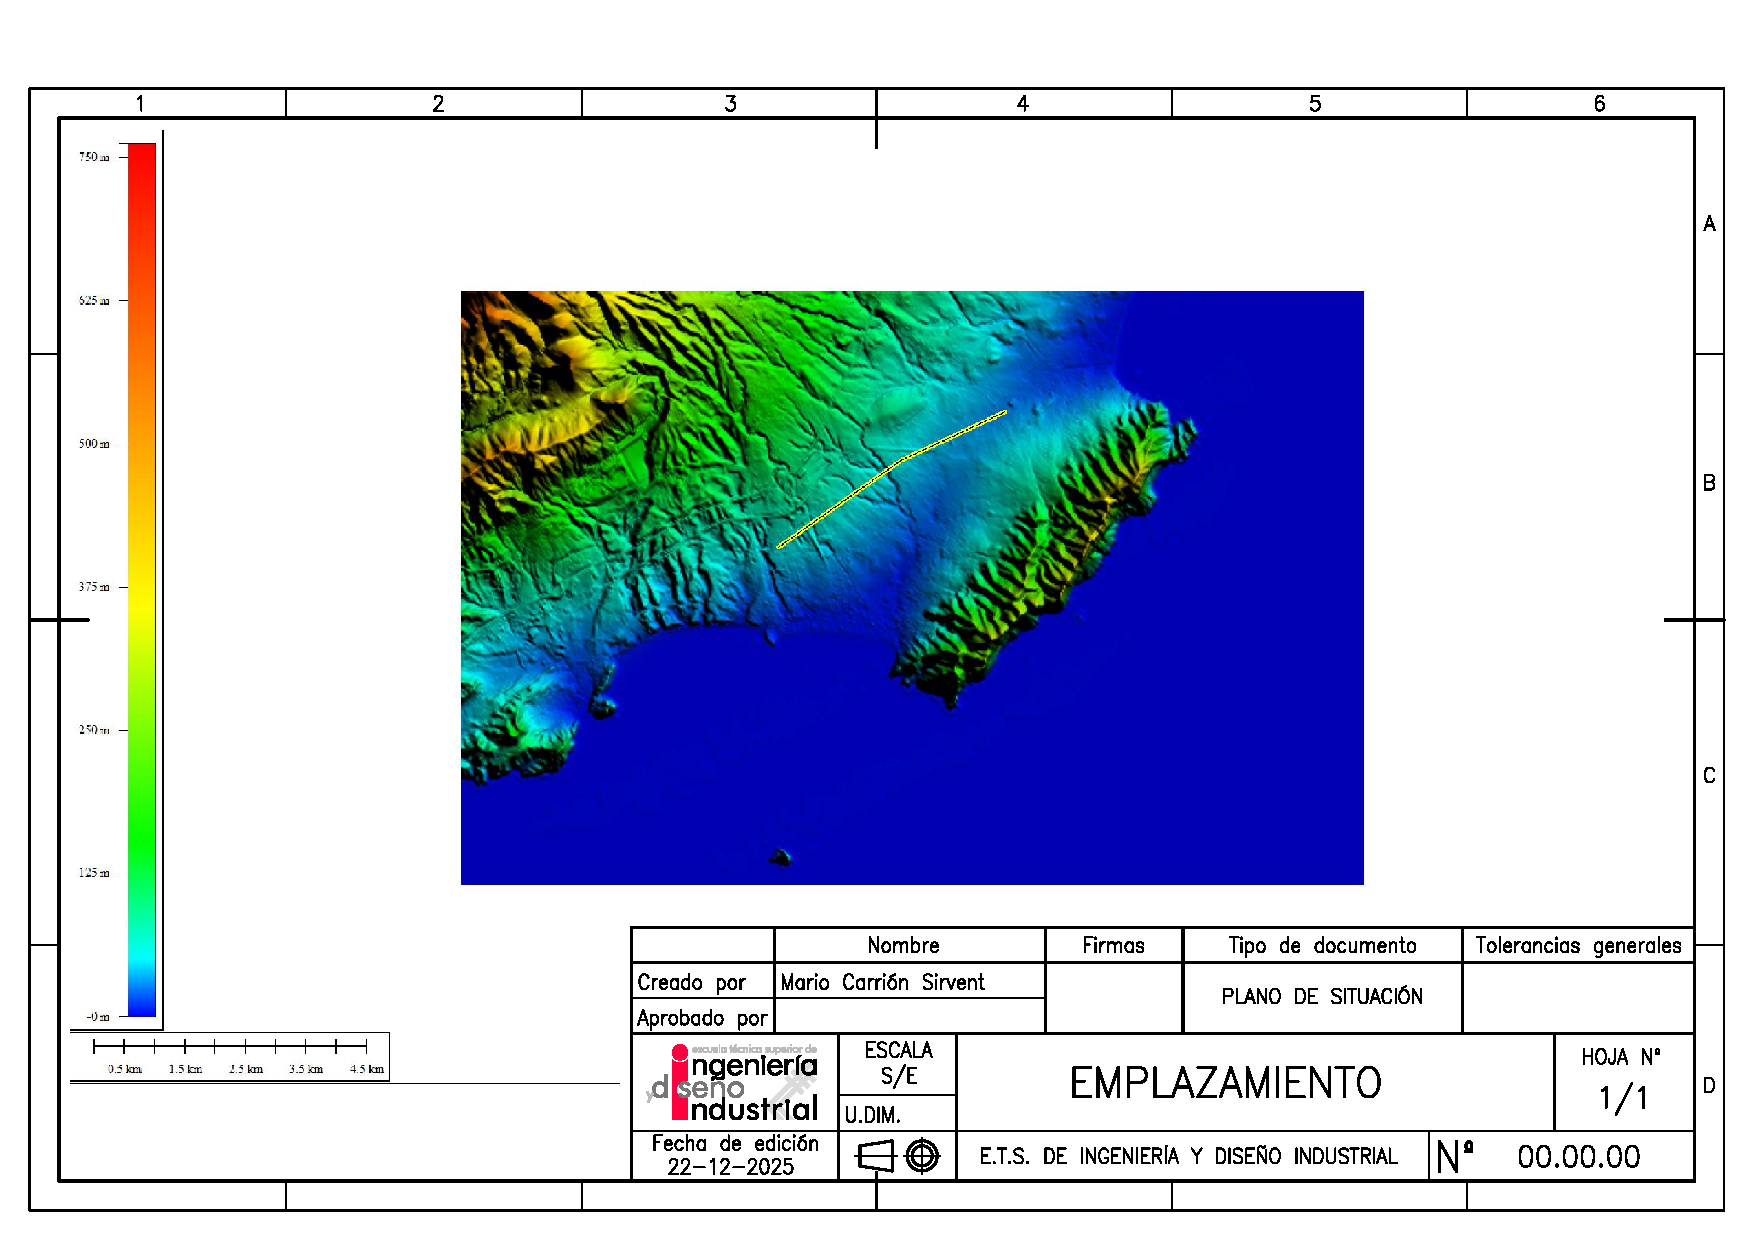
\includepdf[
  pages=-,          
  fitpaper=true, 
]{PDFs/Situacion.pdf}
\section{Perfil longitudinal}
\label{sec:plano-longitudinal}
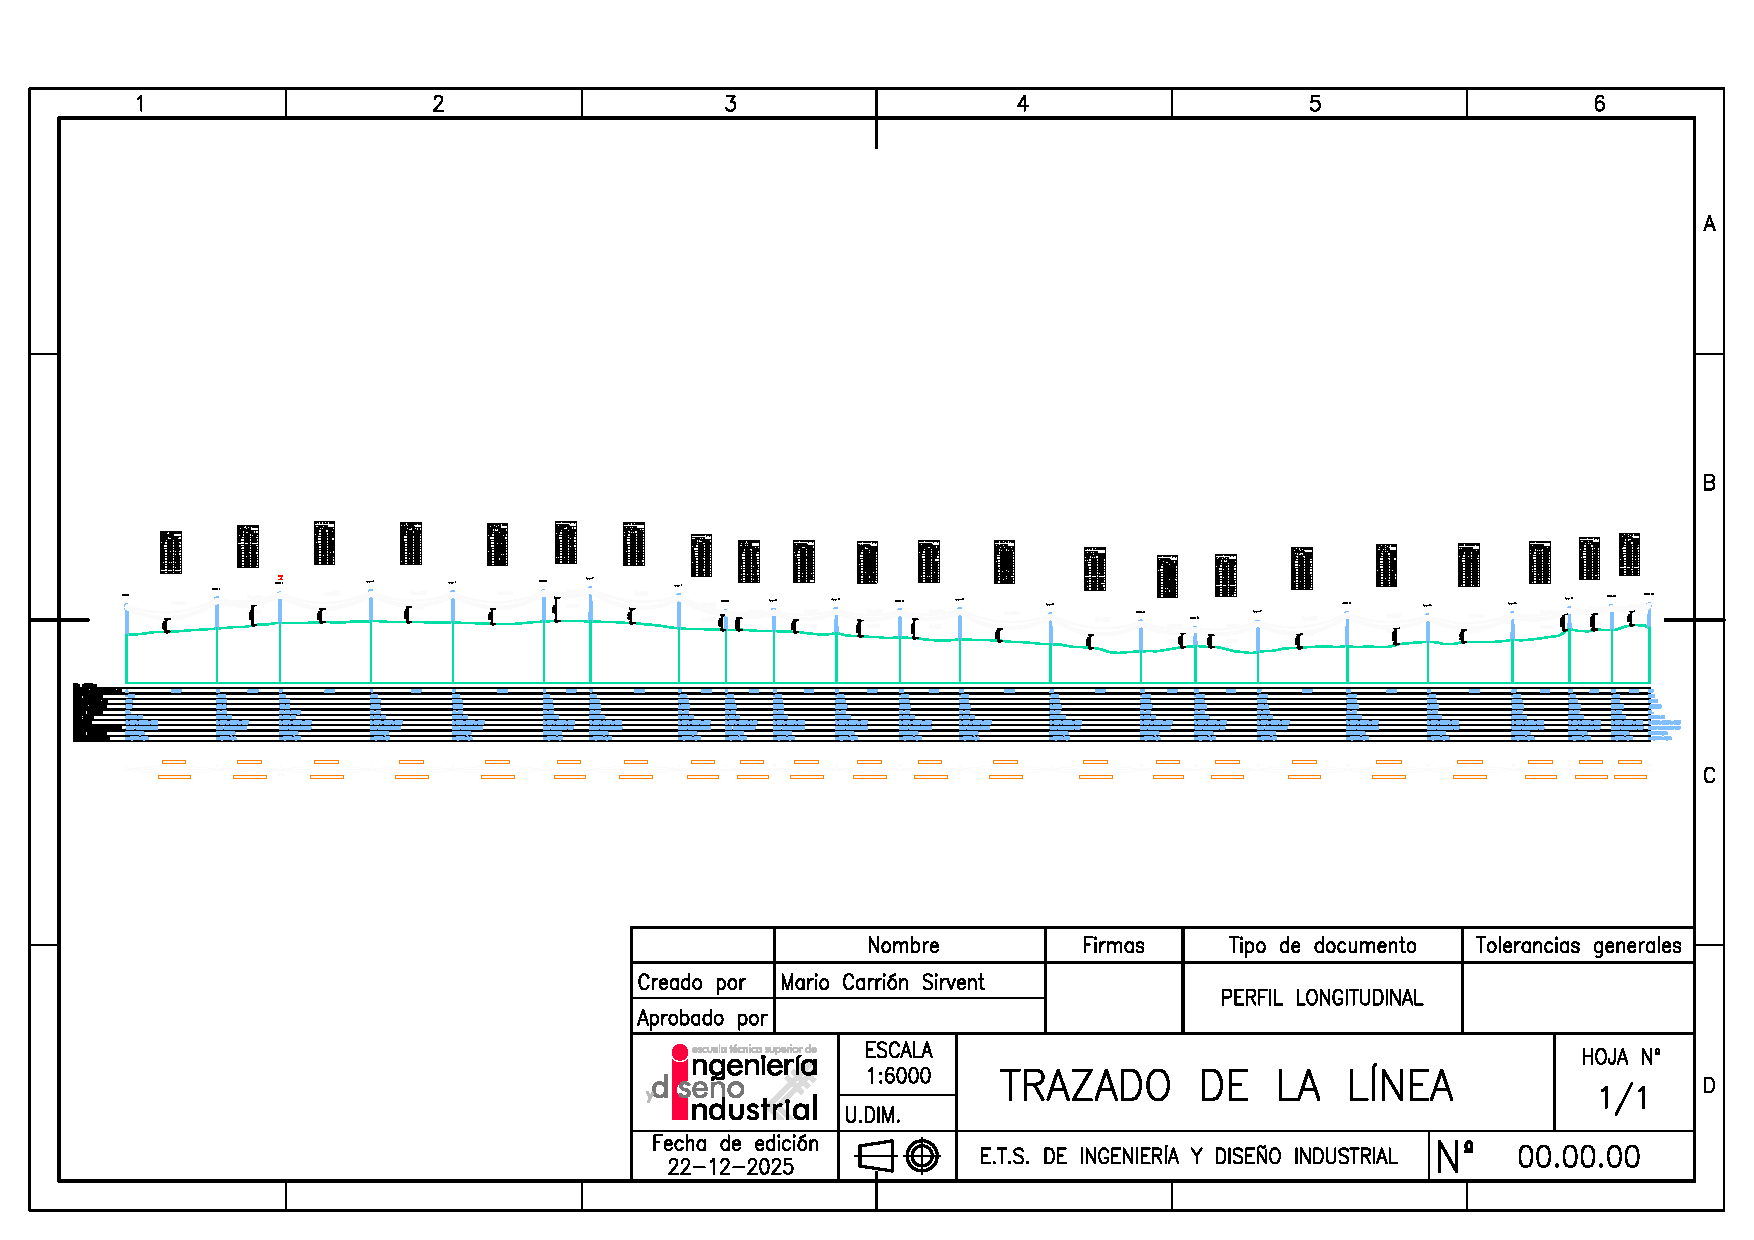
\includepdf[
  pages=-,          
  fitpaper=true,       
]{PDFs/Trazado.pdf}
\section{Alzado completo de la línea}
\label{sec:plano-alzado}
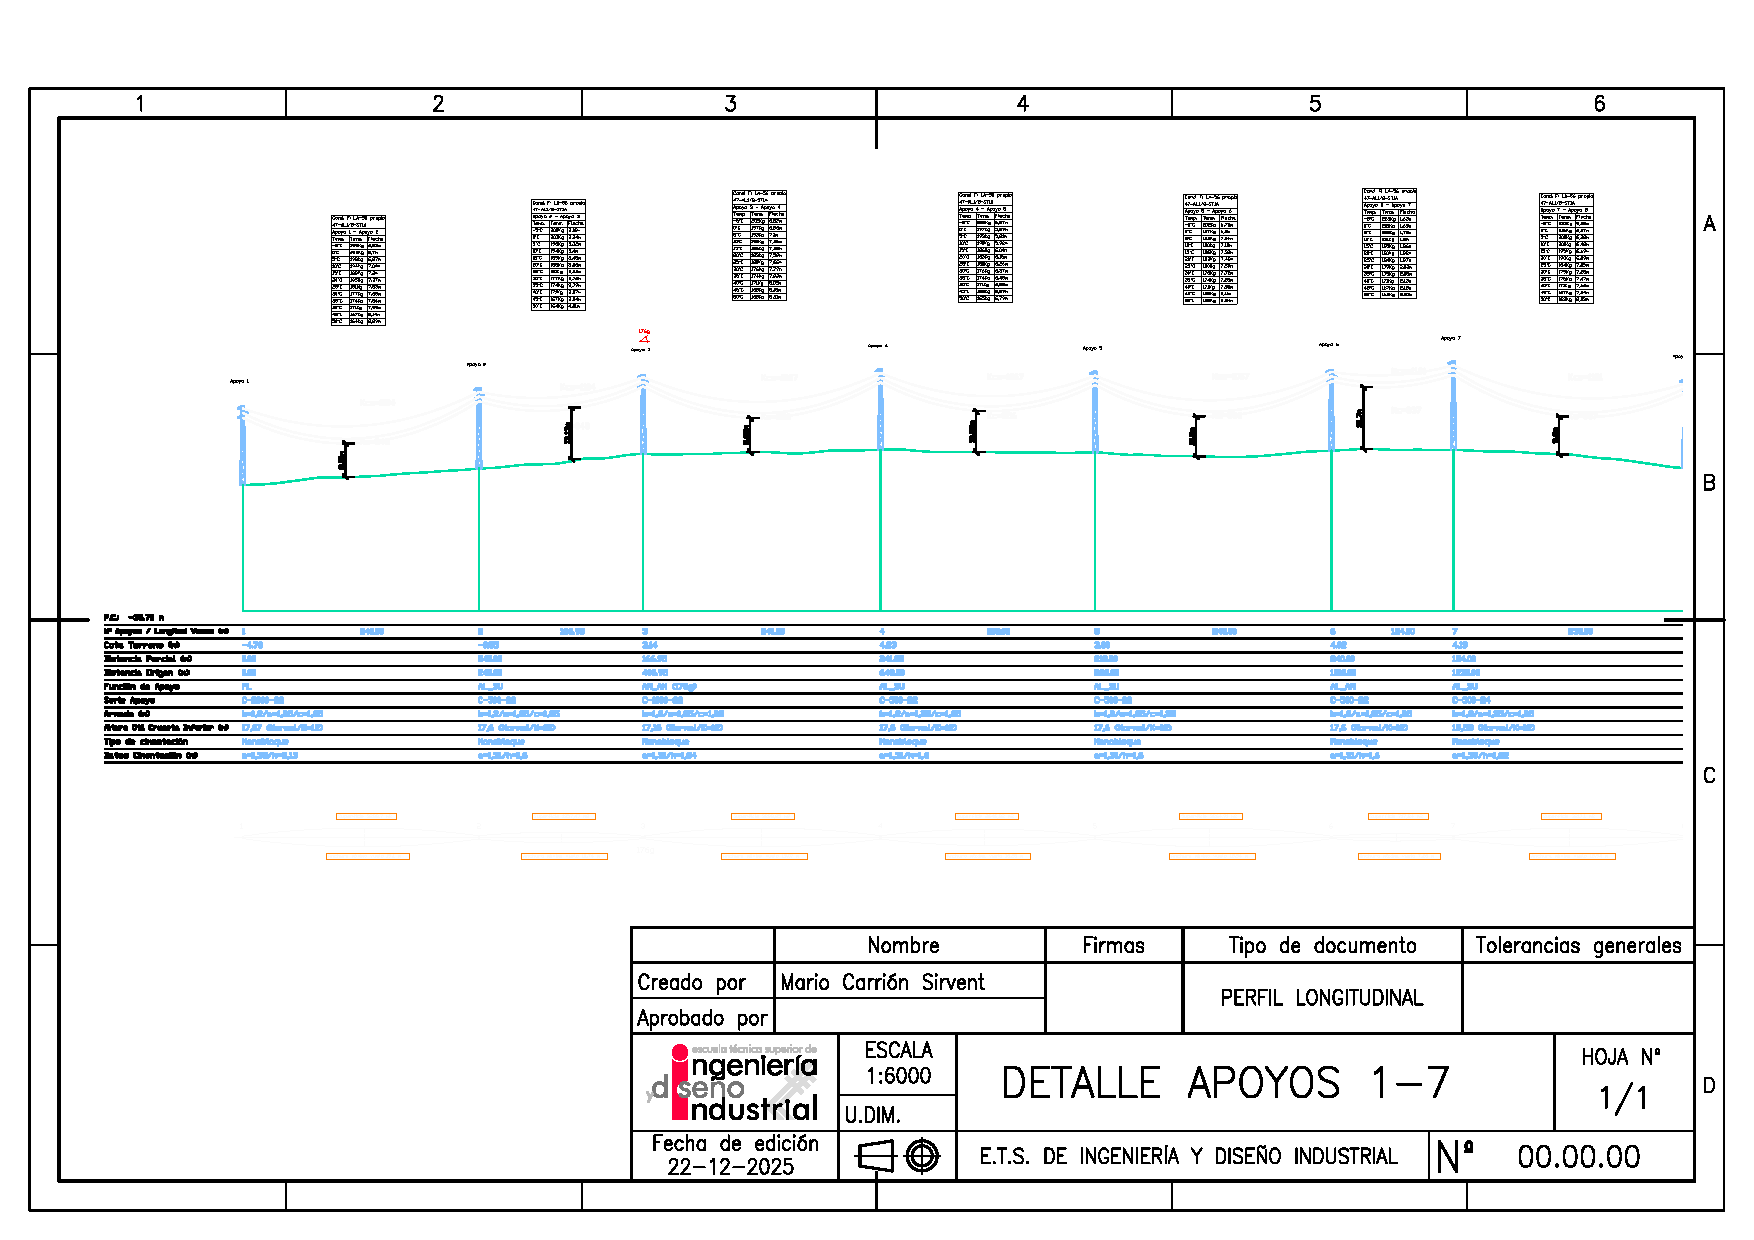
\includepdf[
  pages=-,          
  fitpaper=true,       
]{PDFs/PerfilDef1A4.pdf}

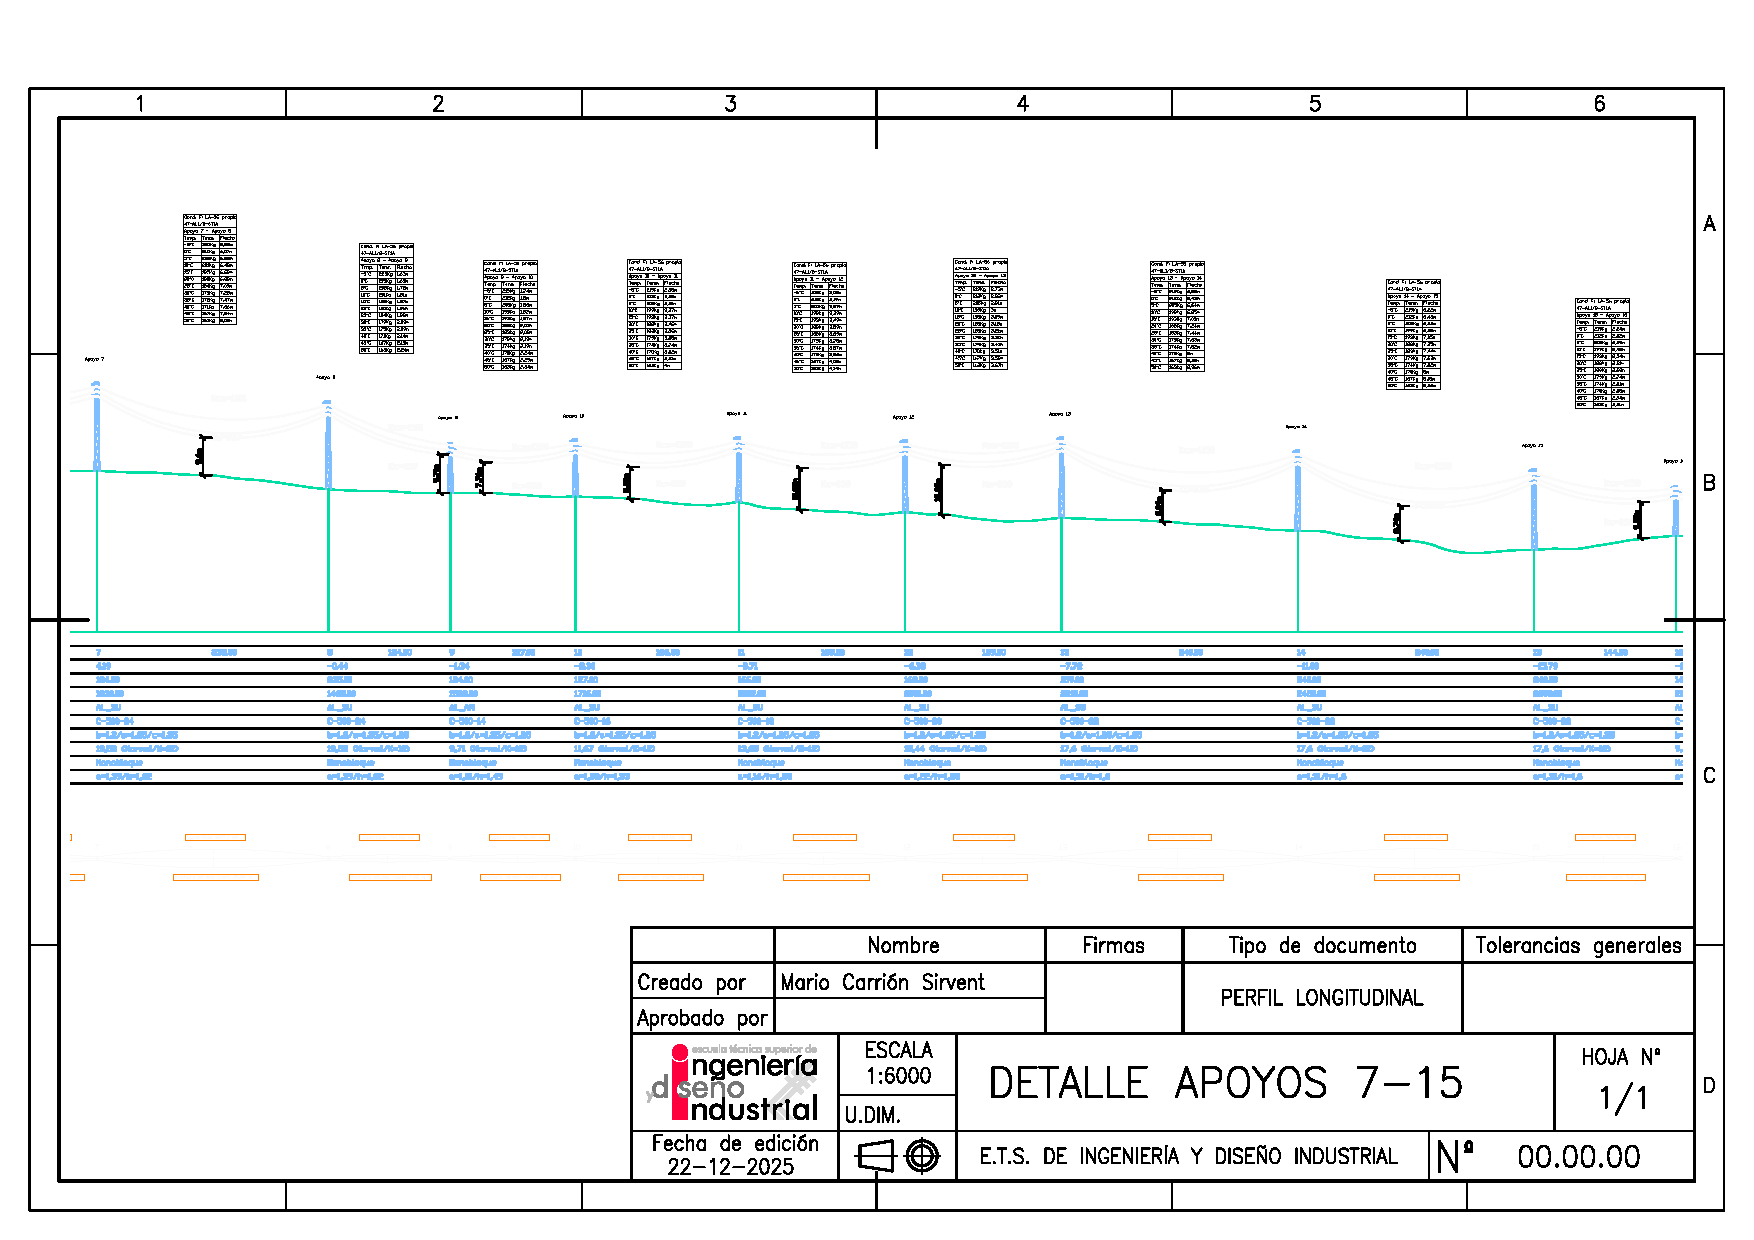
\includepdf[
  pages=-,          
  fitpaper=true,      
]{PDFs/PerfilDef2A4.pdf}

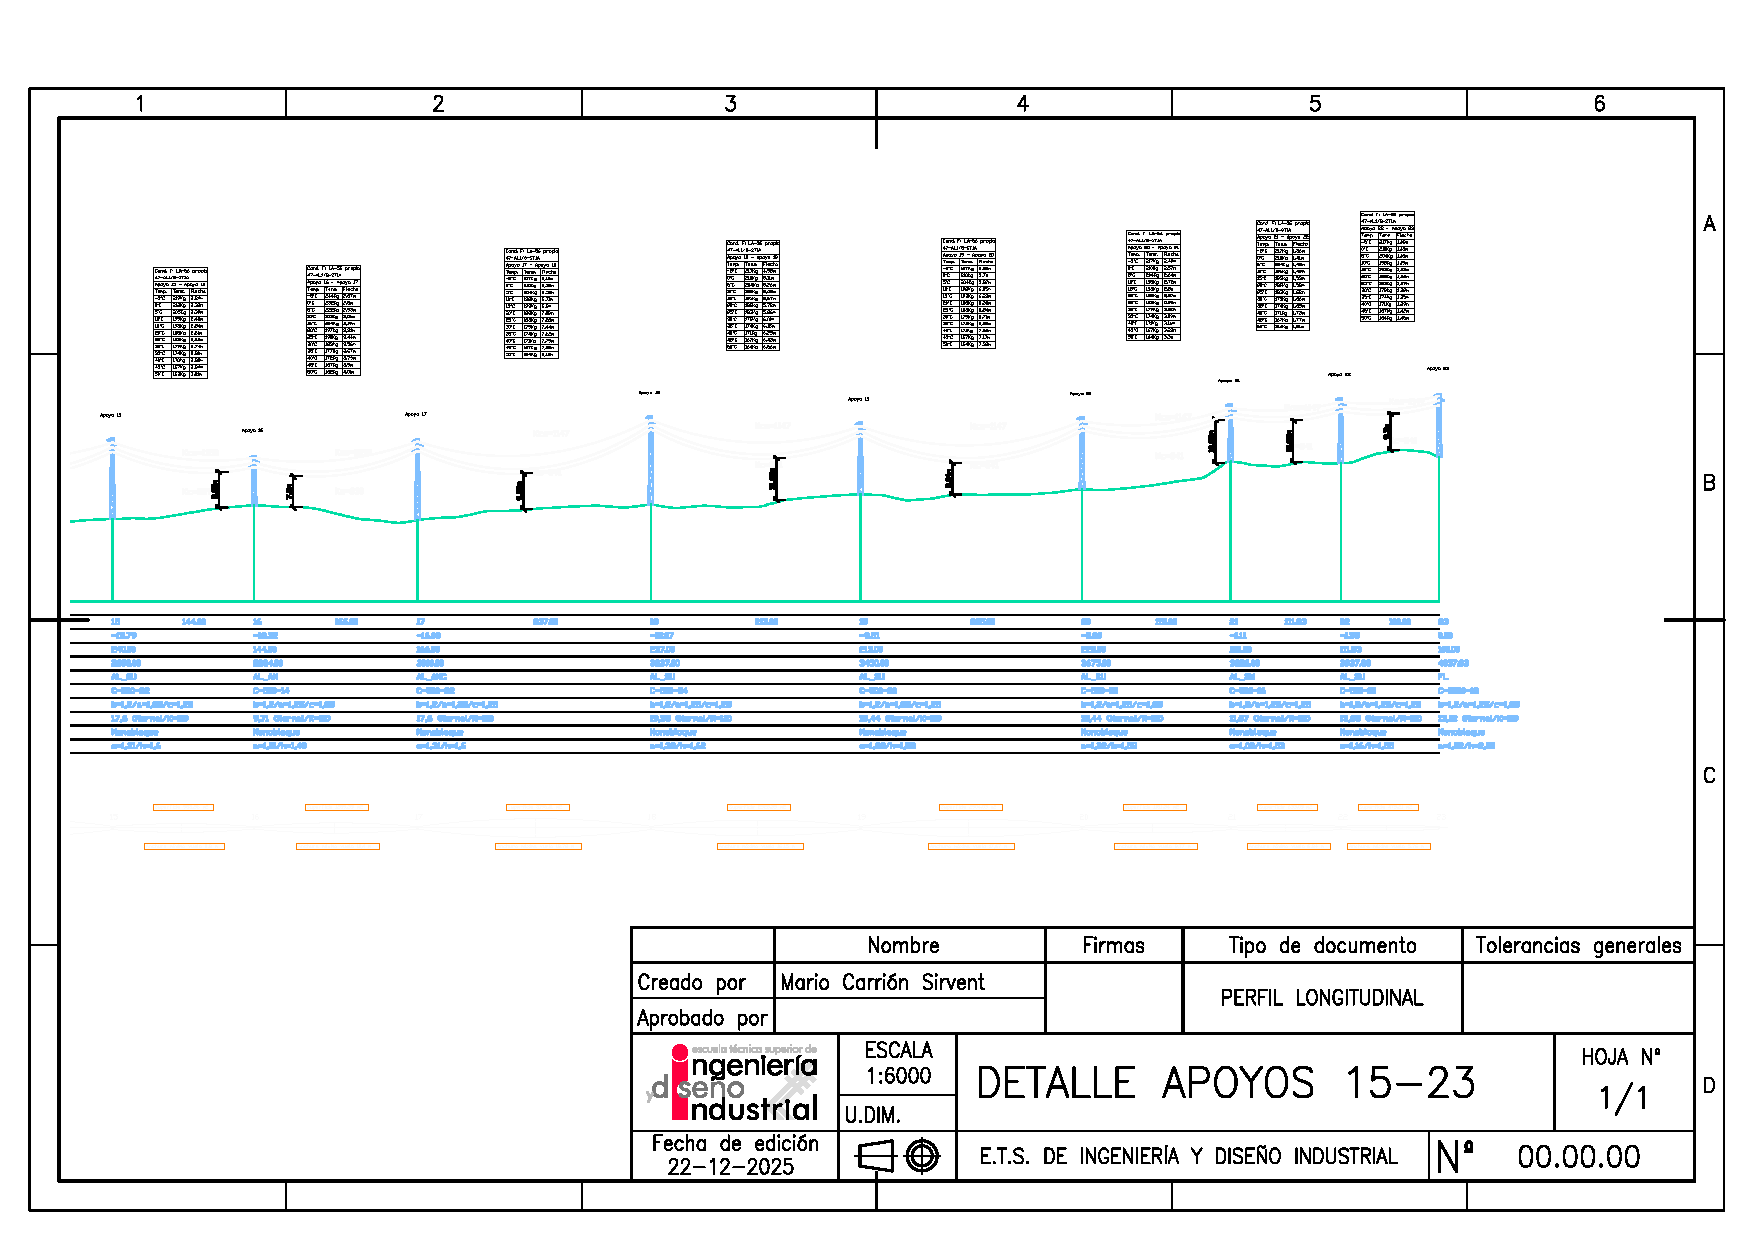
\includepdf[
  pages=-,          
  fitpaper=true,      
]{PDFs/PerfilDef3A4.pdf}
\section{Aislador}
\label{sec:plano-aislador}
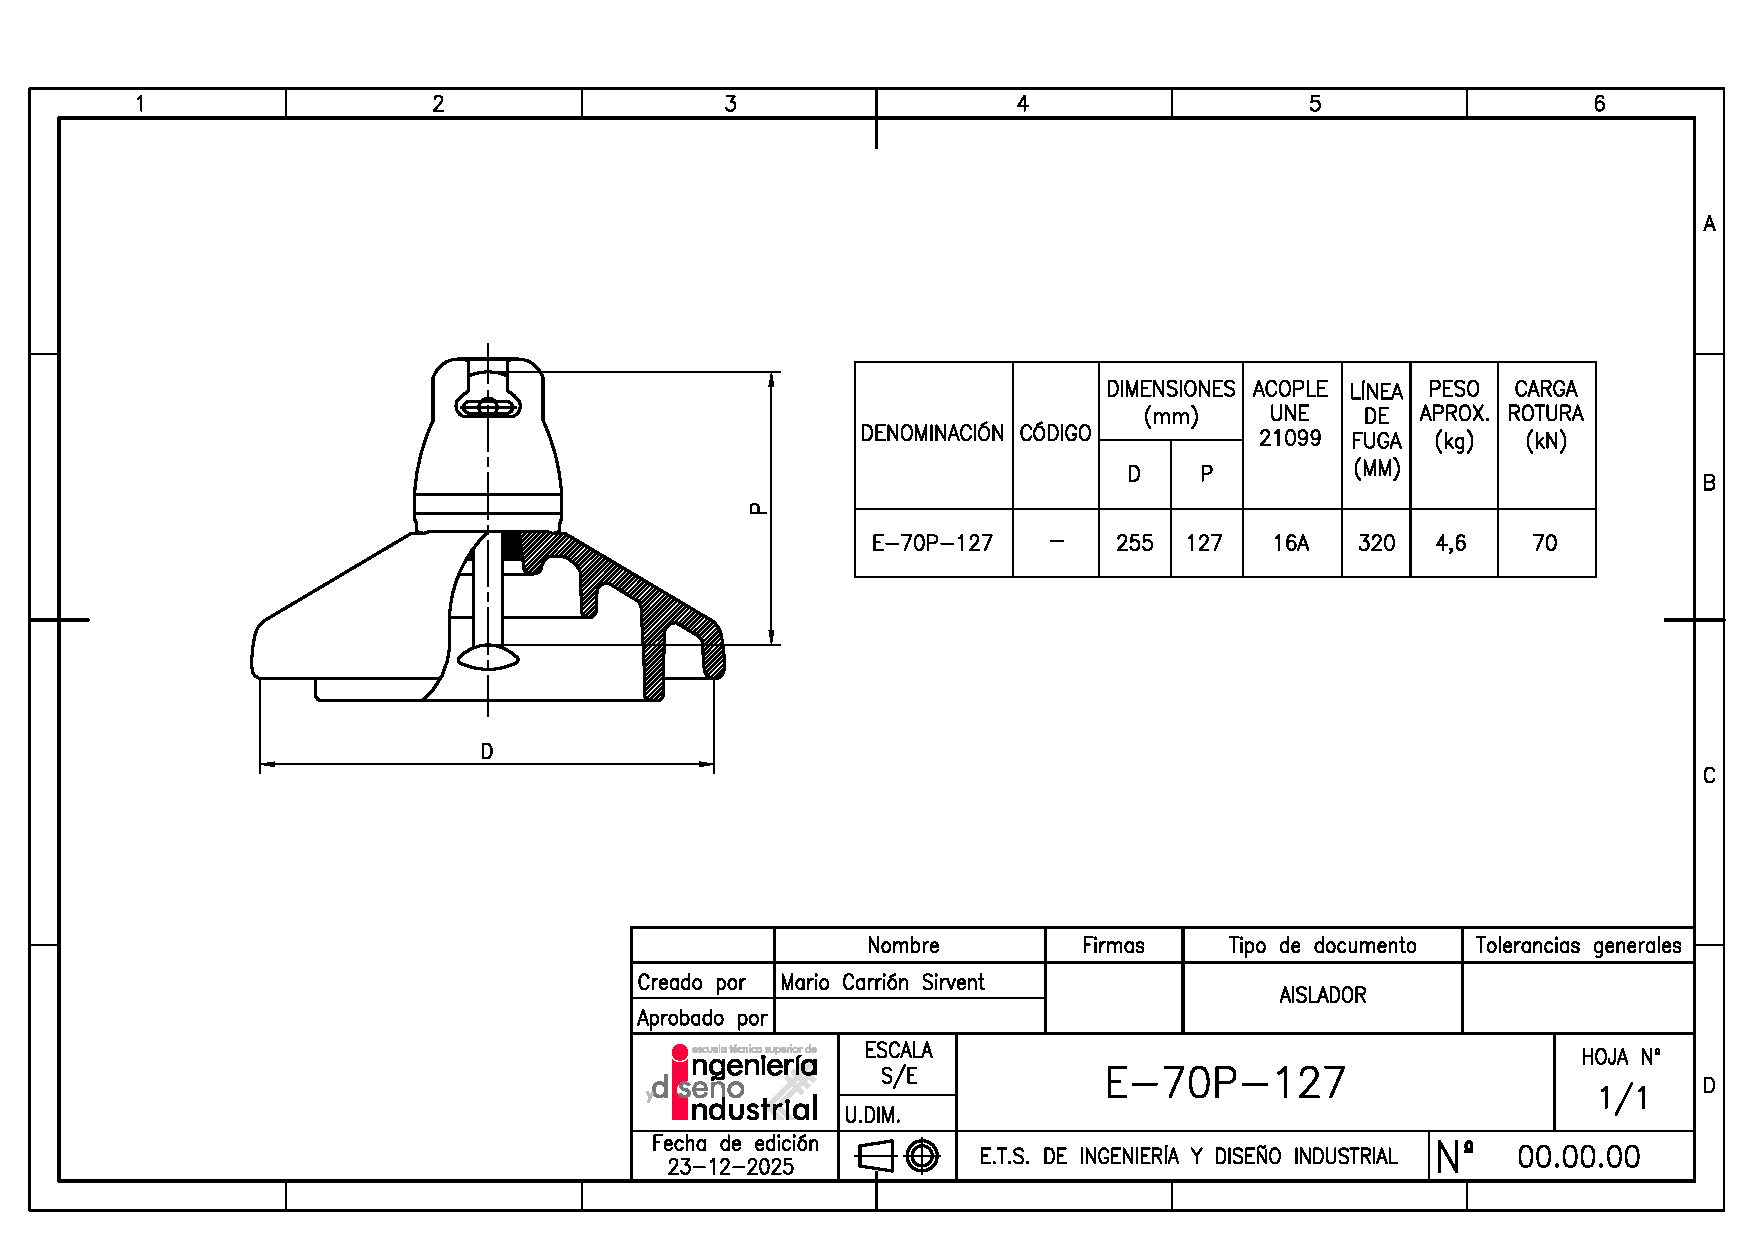
\includepdf[
  pages=-,          
  fitpaper=true,       
]{PDFs/aislador.pdf}
\section{Cadena de aisladores}
\label{sec:plano-cadenas}
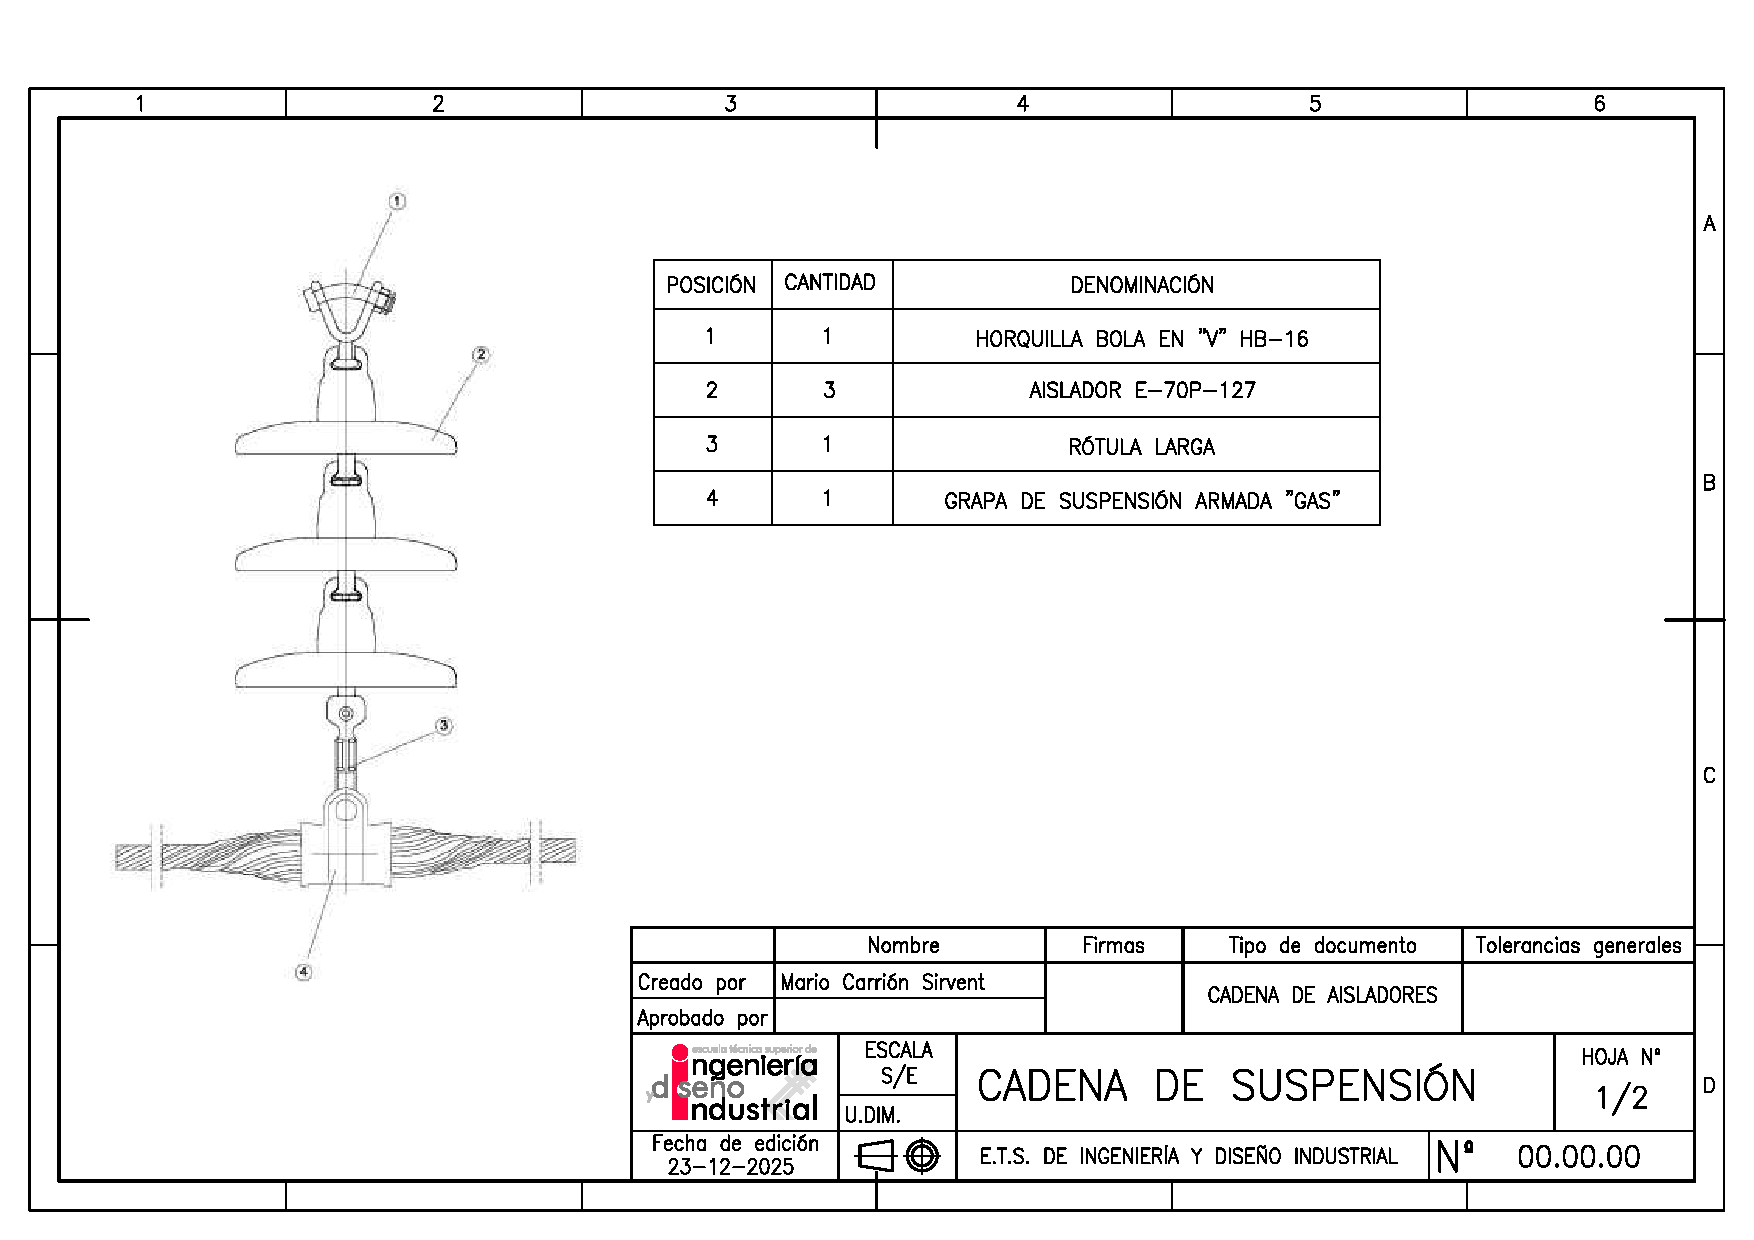
\includepdf[
  pages=-,          
  fitpaper=true,      
]{PDFs/cadena-suspension.pdf}

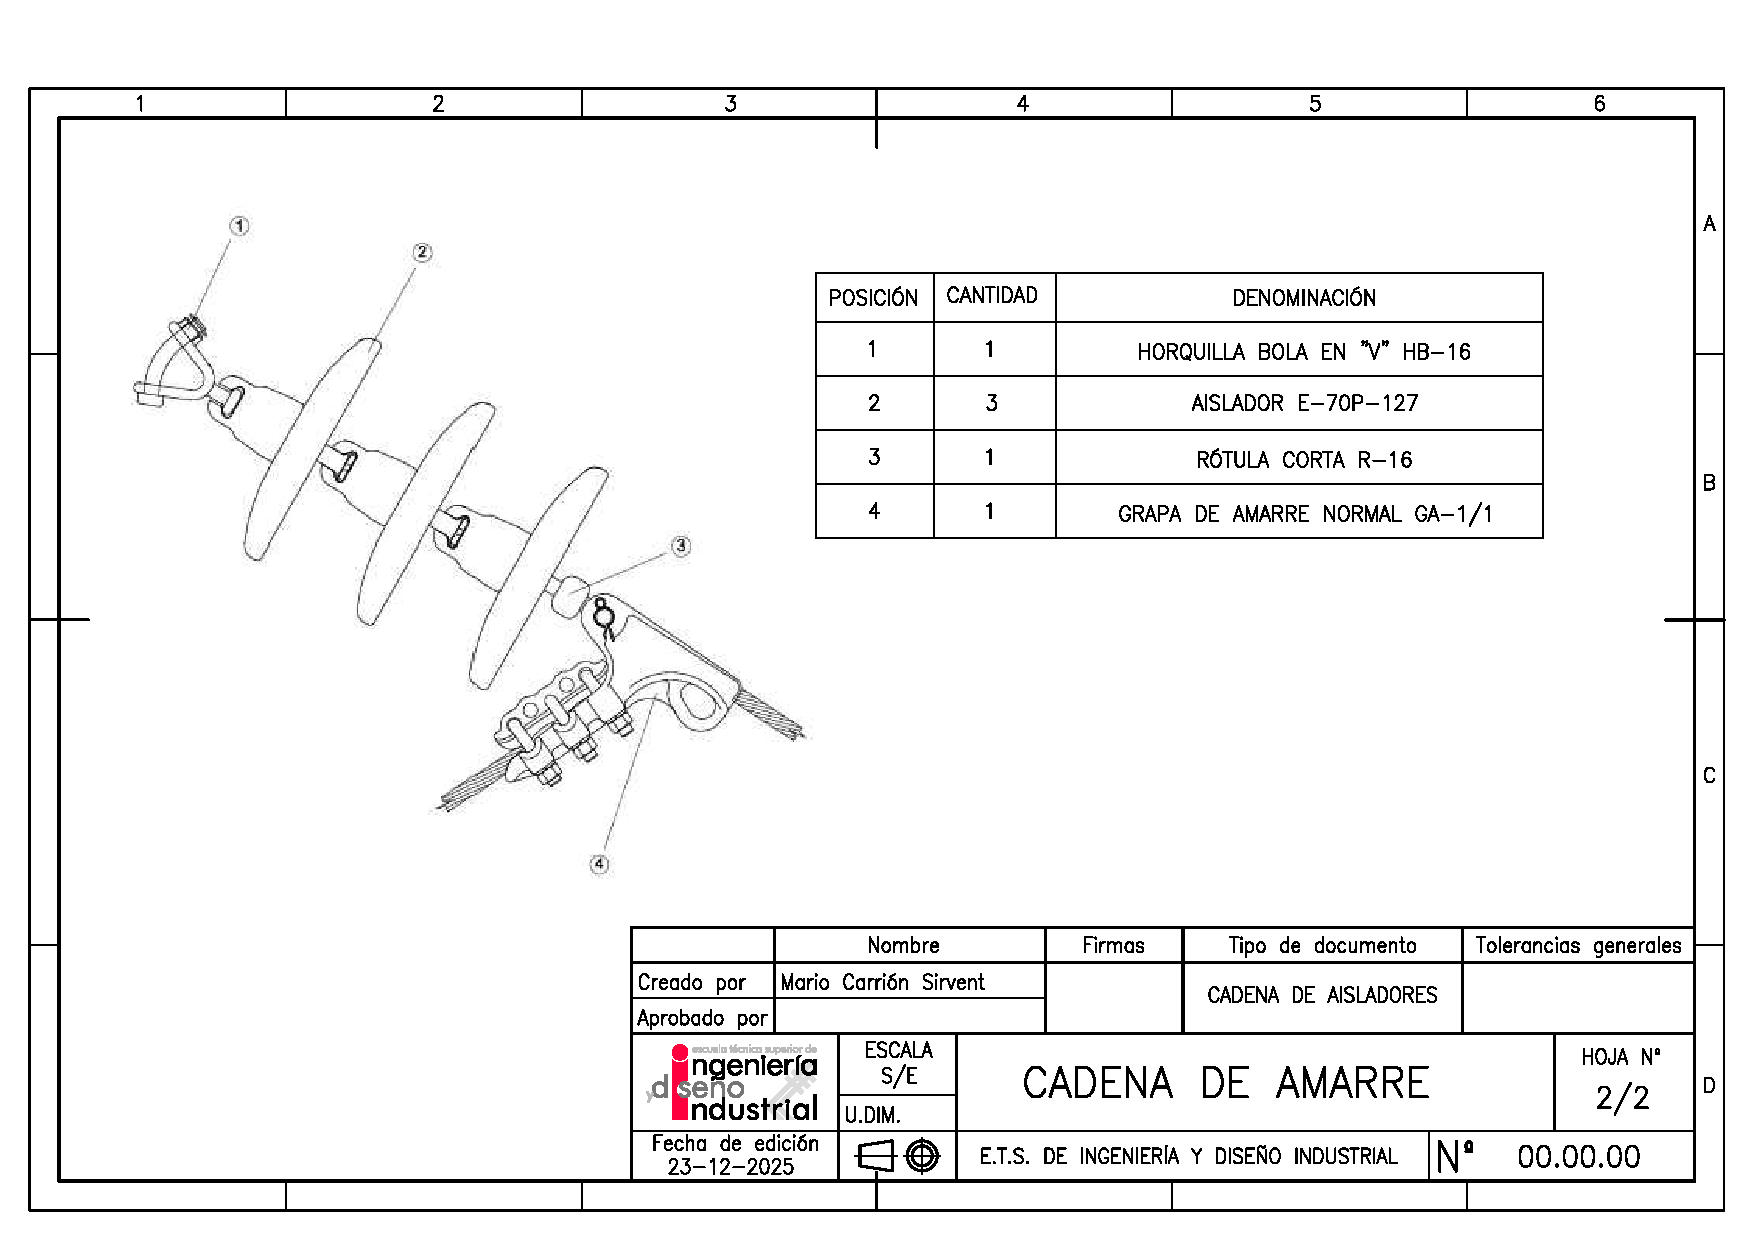
\includepdf[
  pages=-,          
  fitpaper=true,      
]{PDFs/cadena-amarre.pdf}
\section{Cimentaciones}
\label{sec:plano-cimentaciones}
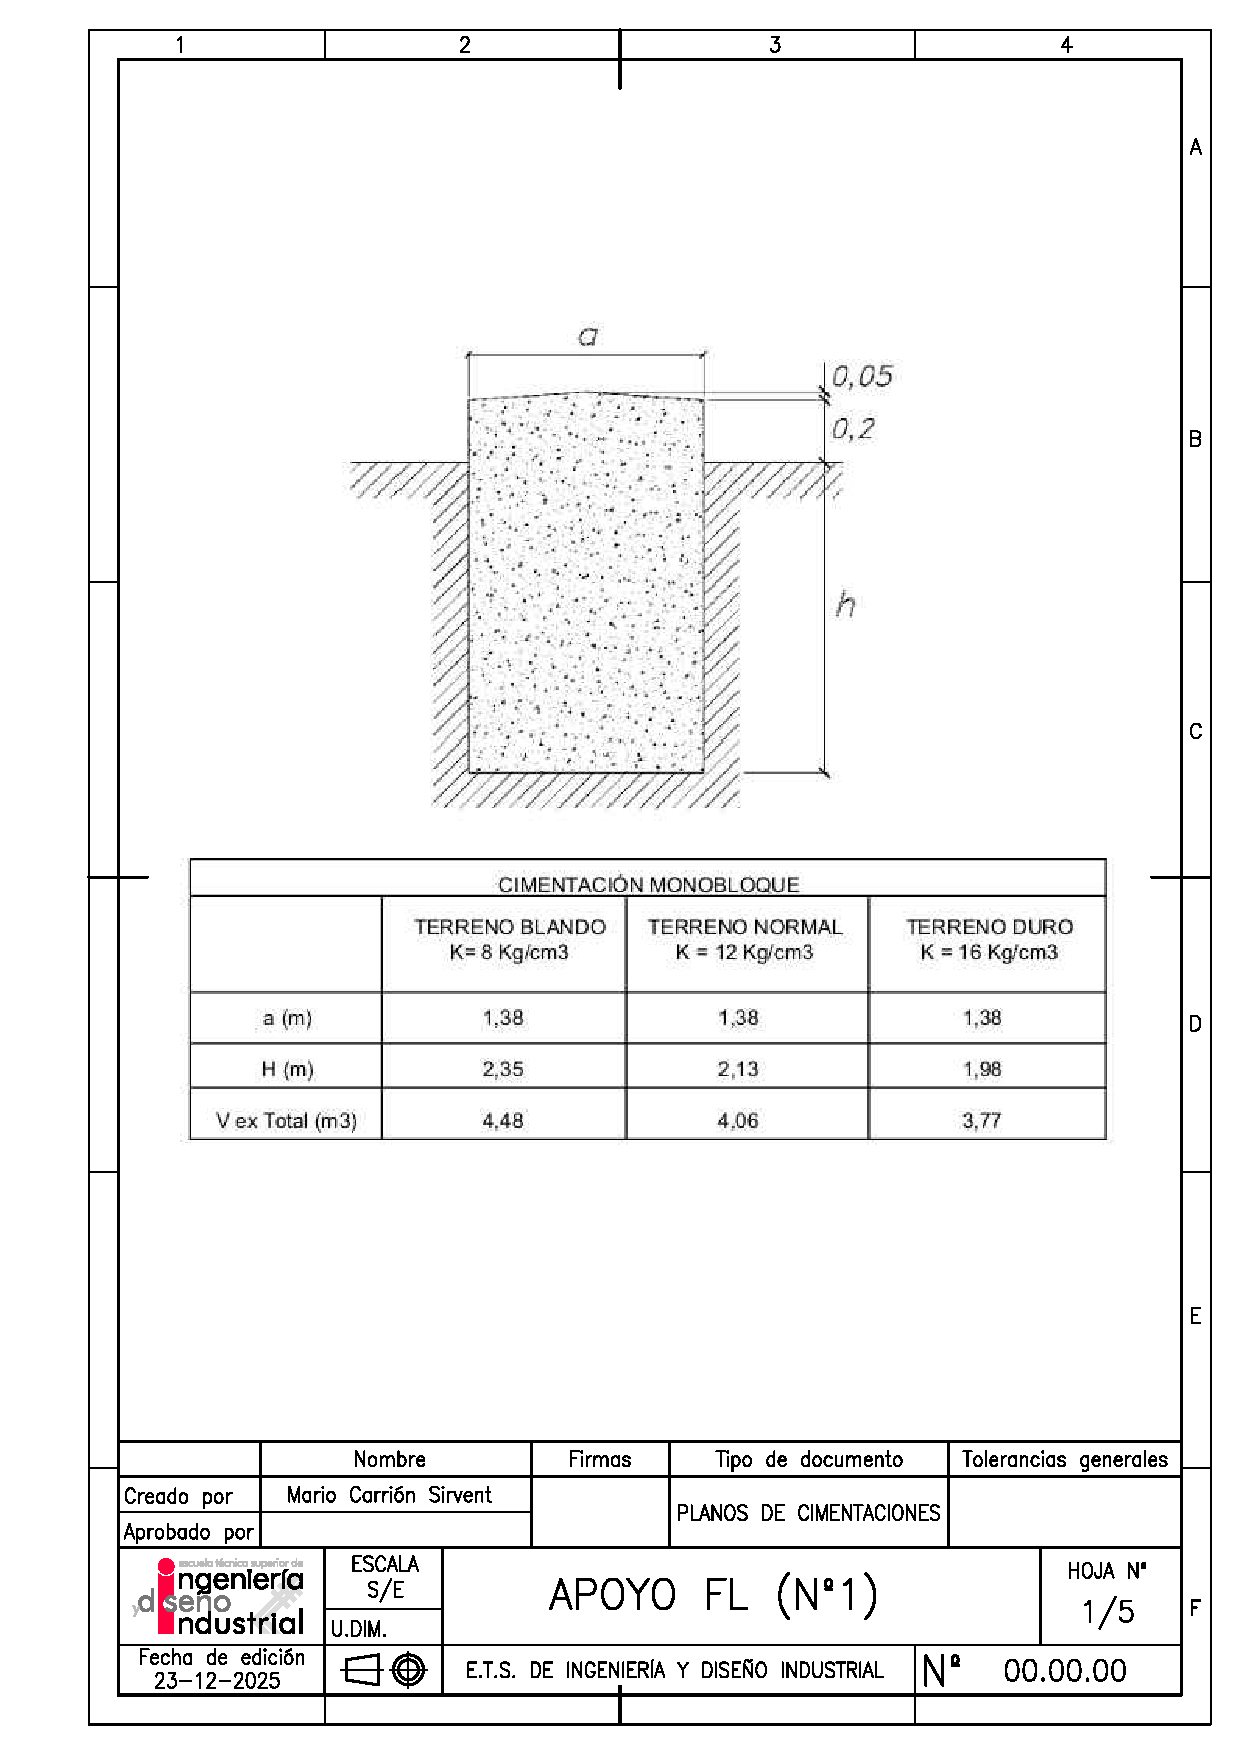
\includepdf[
  pages=-,          
  fitpaper=true,     
]{PDFs/cim-FL.pdf}

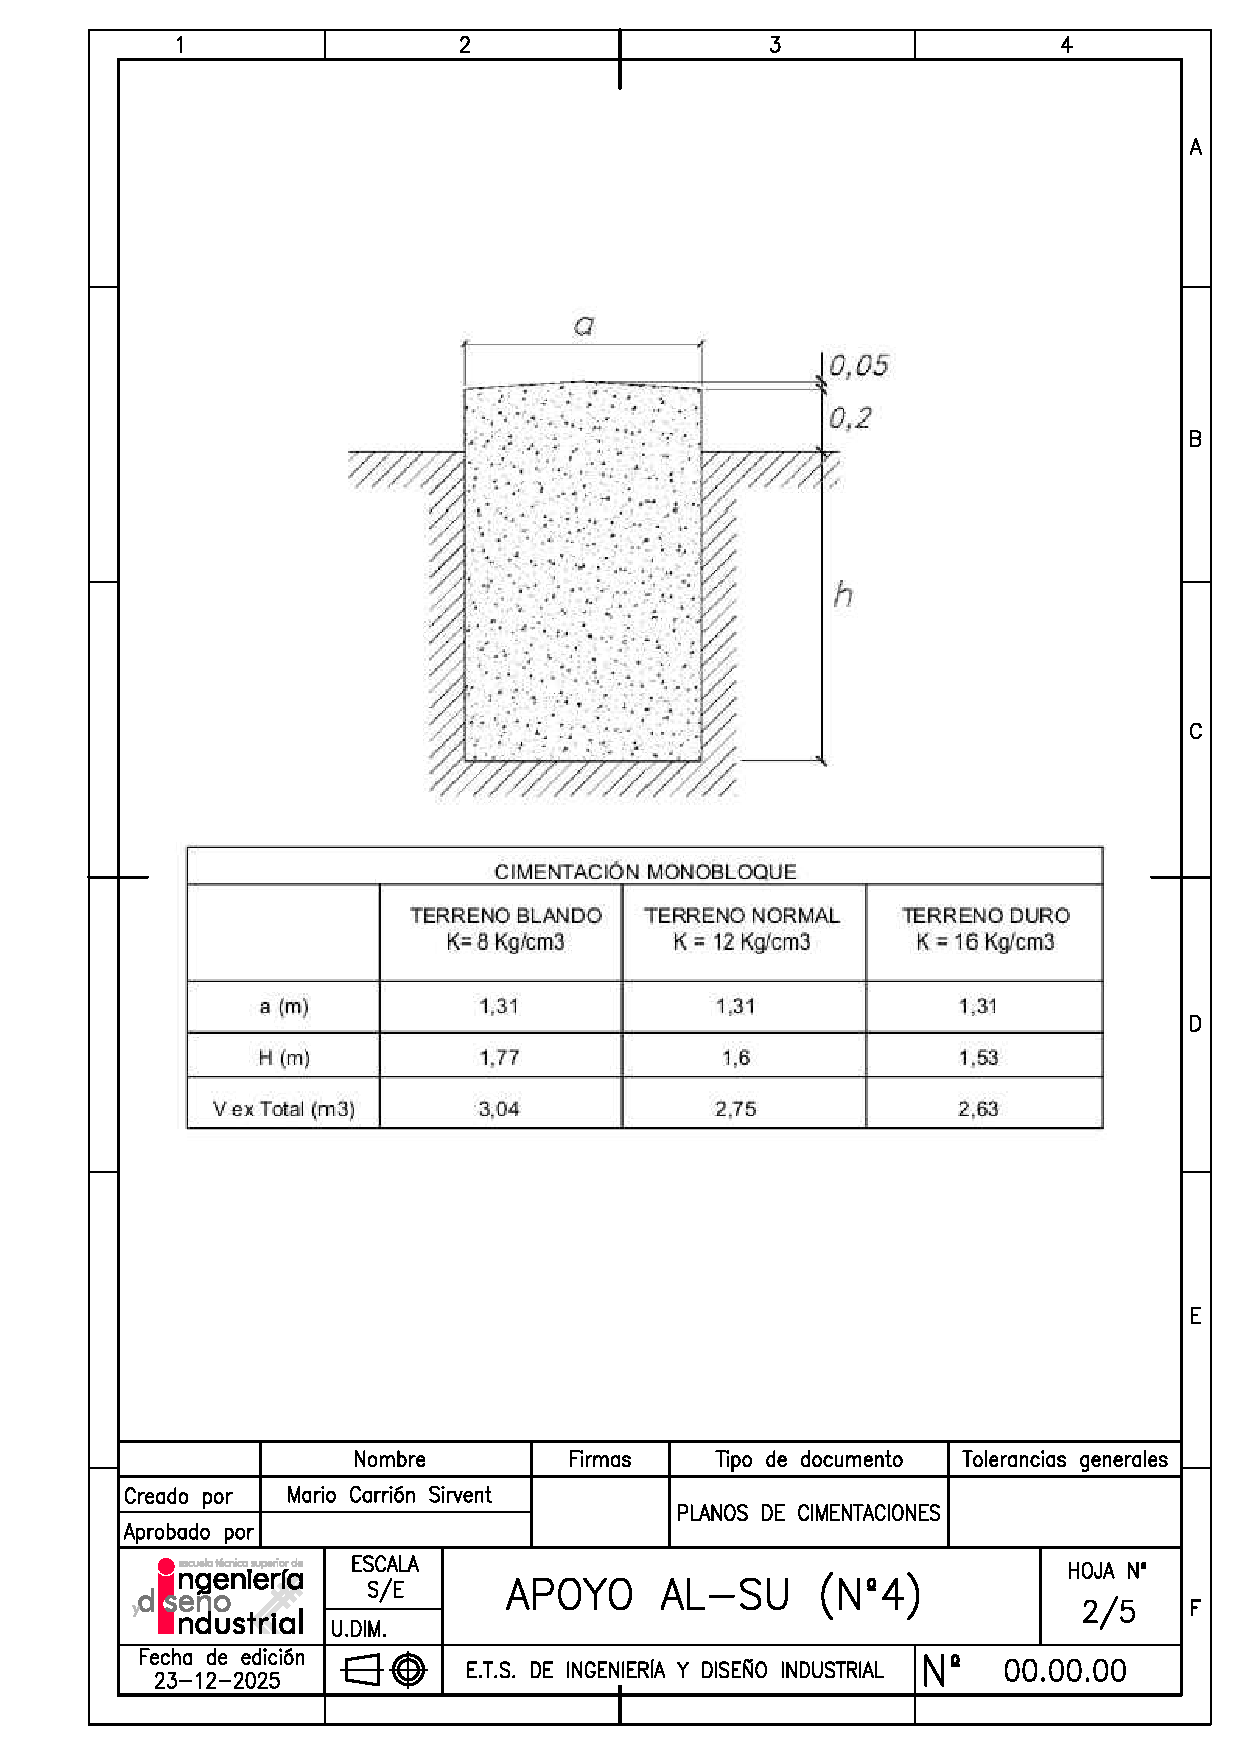
\includepdf[
  pages=-,          
  fitpaper=true,       
]{PDFs/cim-ALSU.pdf}

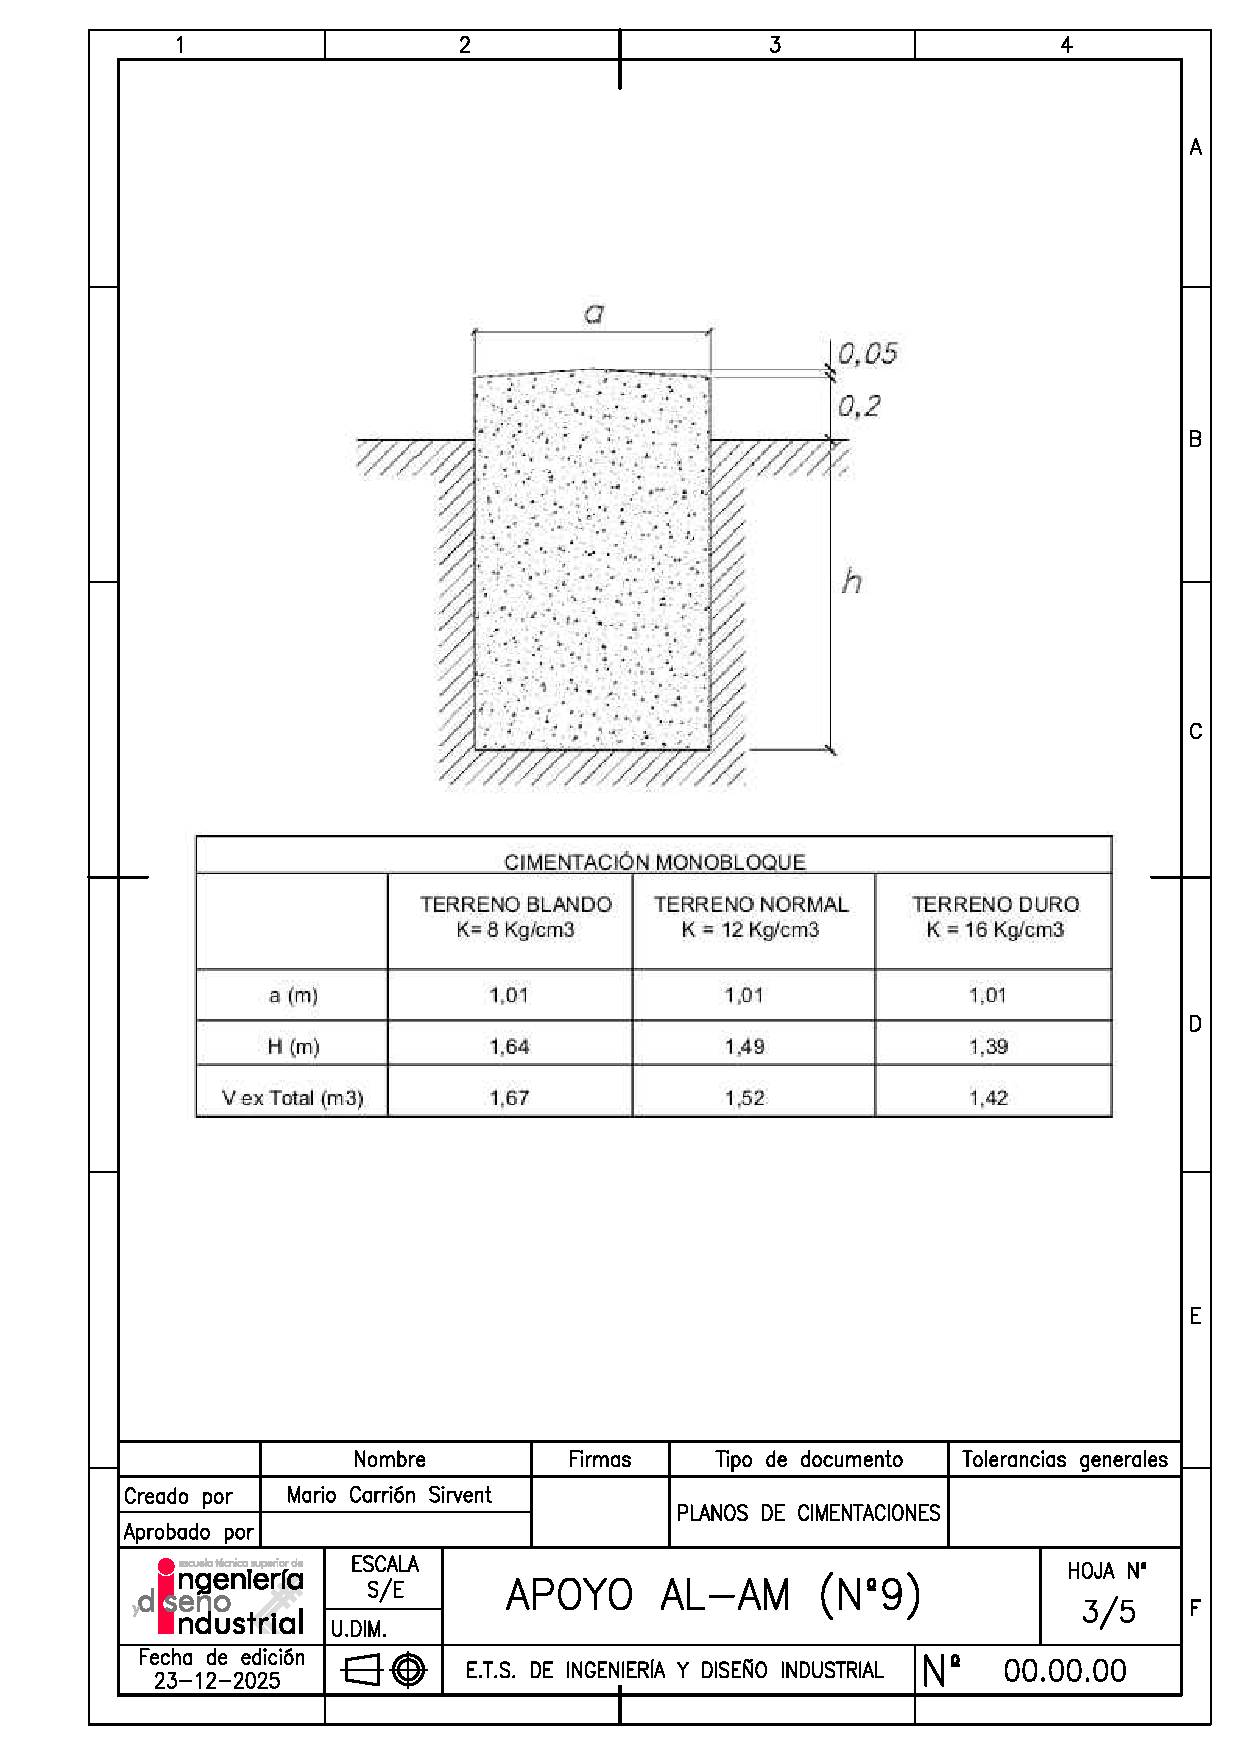
\includepdf[
  pages=-,          
  fitpaper=true,       
]{PDFs/cim-ALAM.pdf}

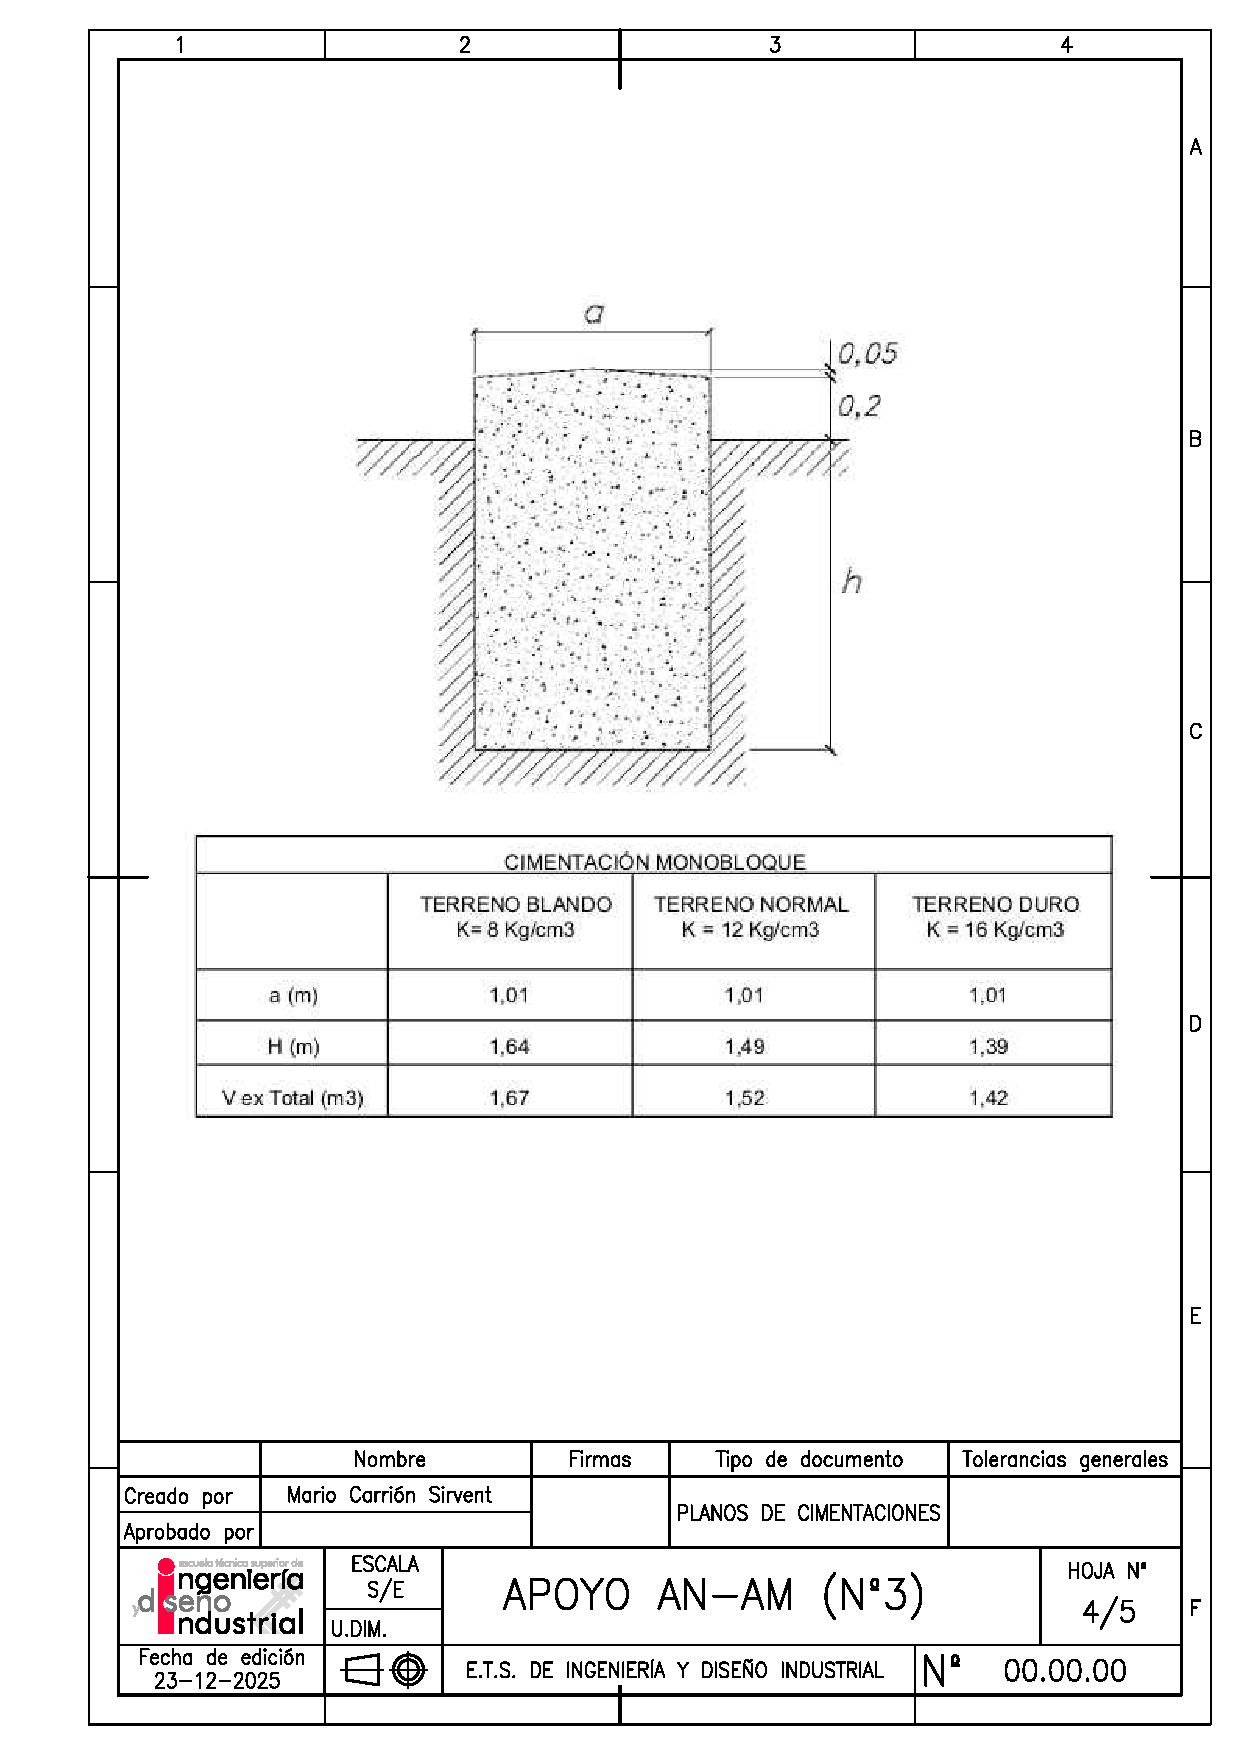
\includepdf[
  pages=-,          
  fitpaper=true,      
]{PDFs/cim-ANAM.pdf}

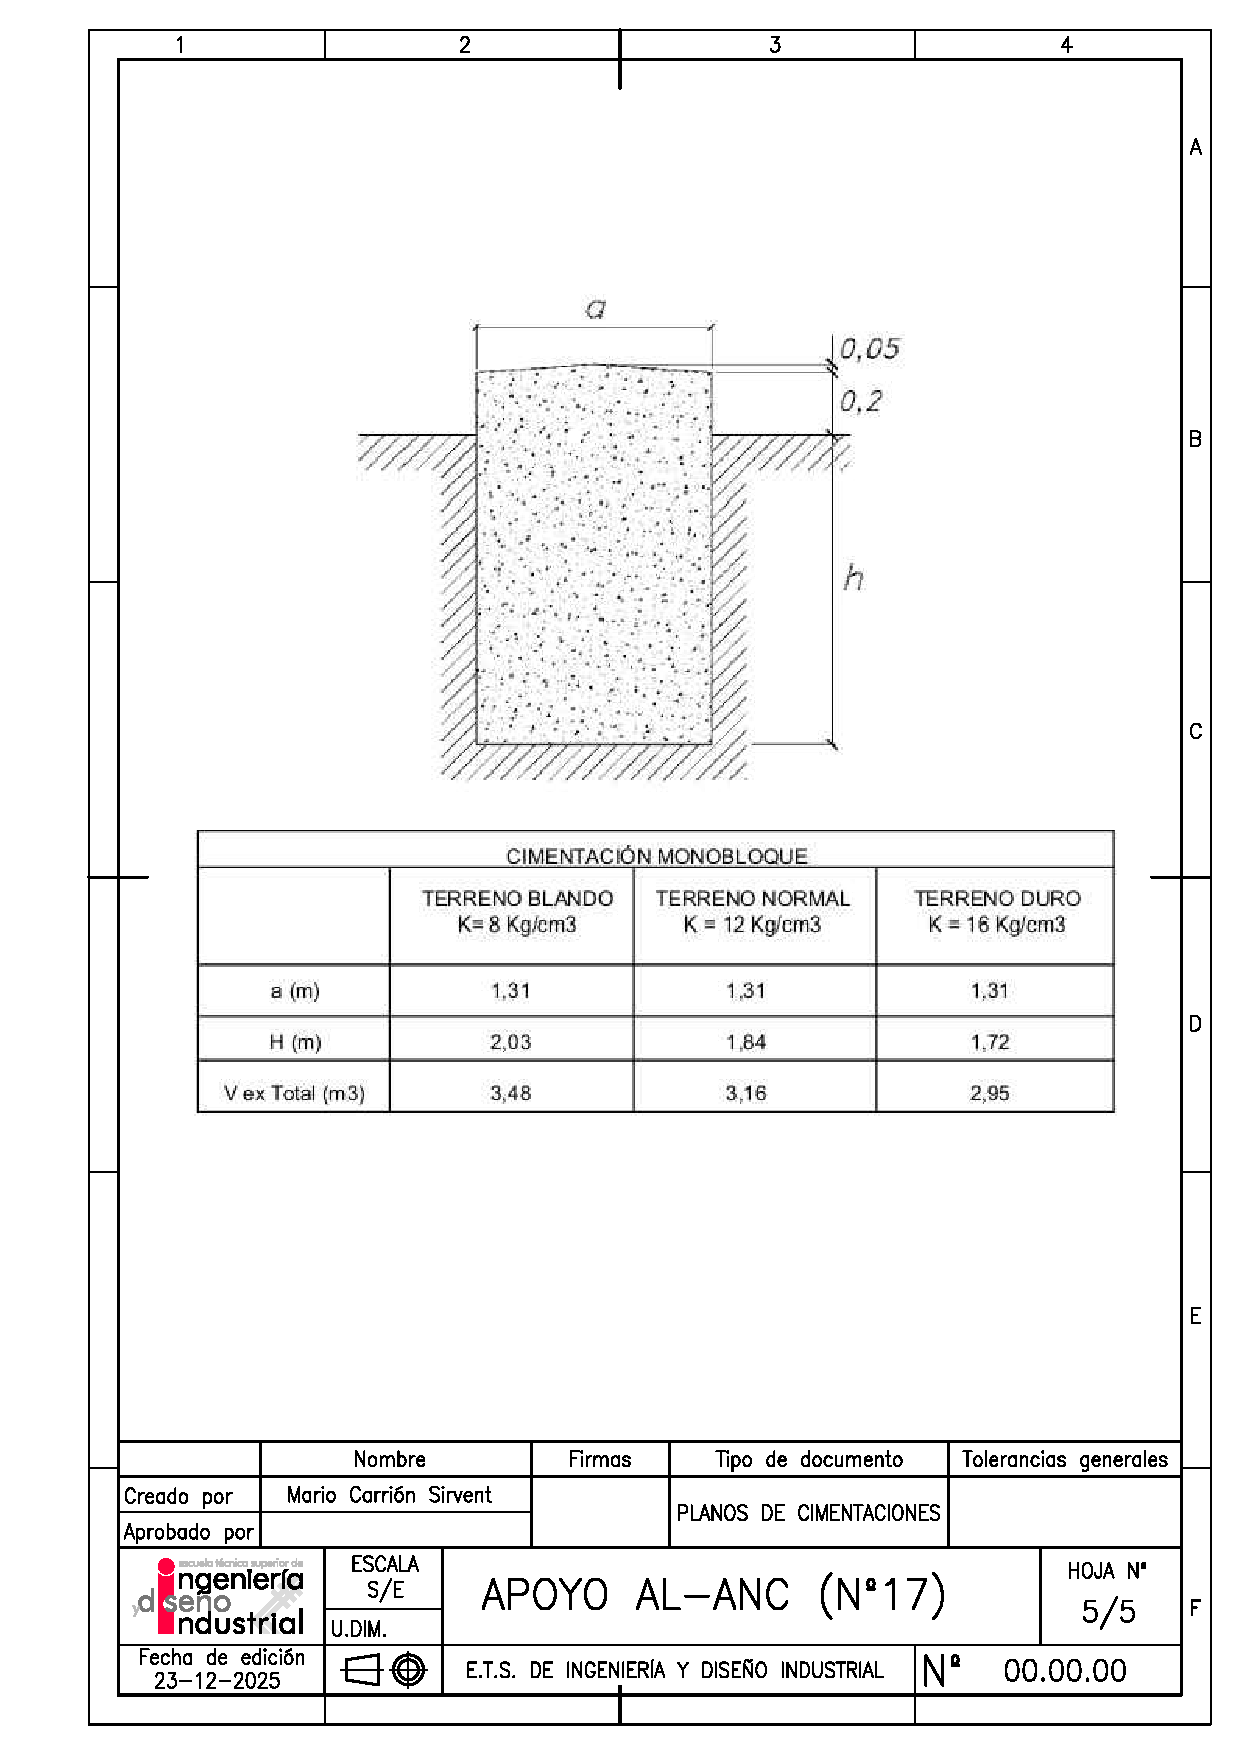
\includepdf[
  pages=-,          
  fitpaper=true,     
]{PDFs/cim-ALANC.pdf}
\section{Diseño de PAT de un apoyo frecuentado con calzado}
\label{sec:plano-pat-frecuentado}
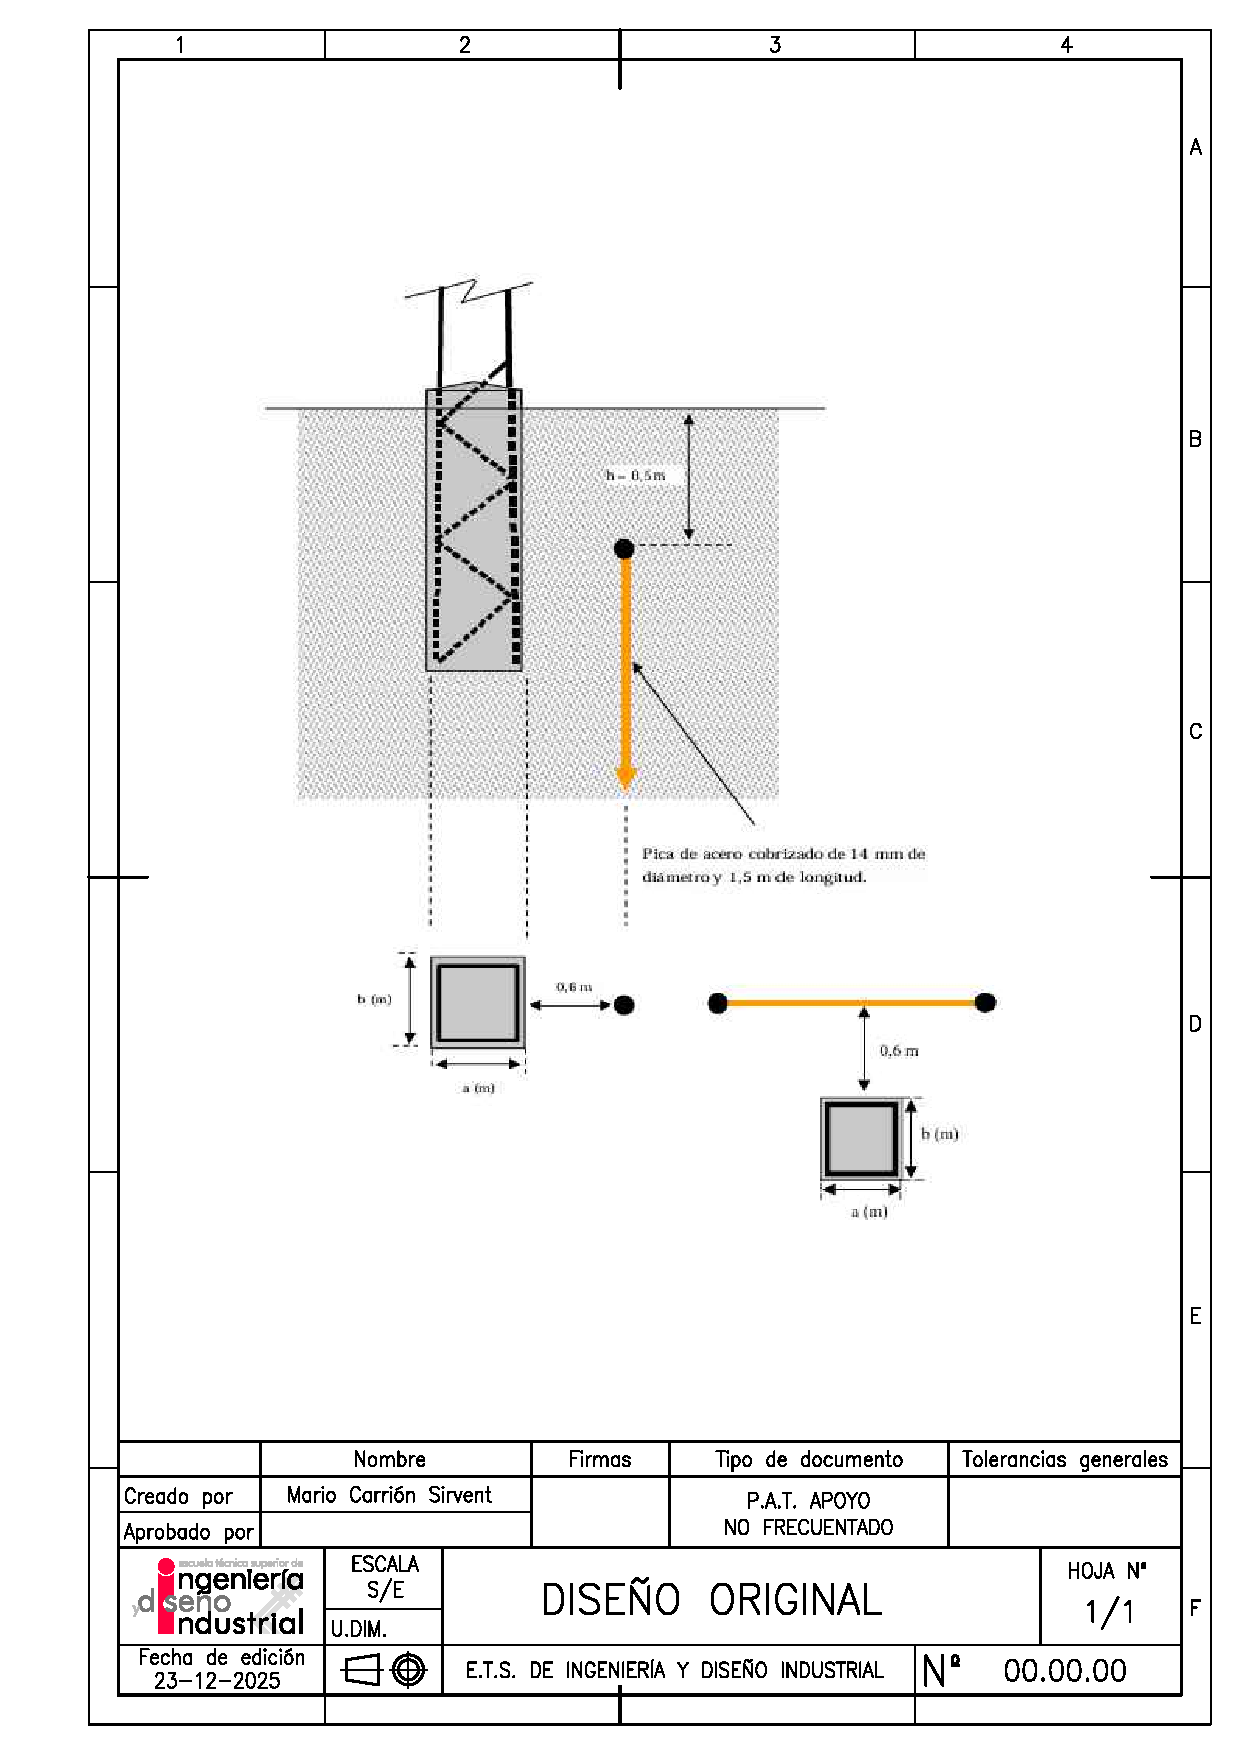
\includepdf[
  pages=-,          
  fitpaper=true,     
]{PDFs/pat-apoyoNF.pdf}
\section{Diseño de PAT de un apoyo no frecuentado}
\label{sec:plano-pat-nofrecuentado}
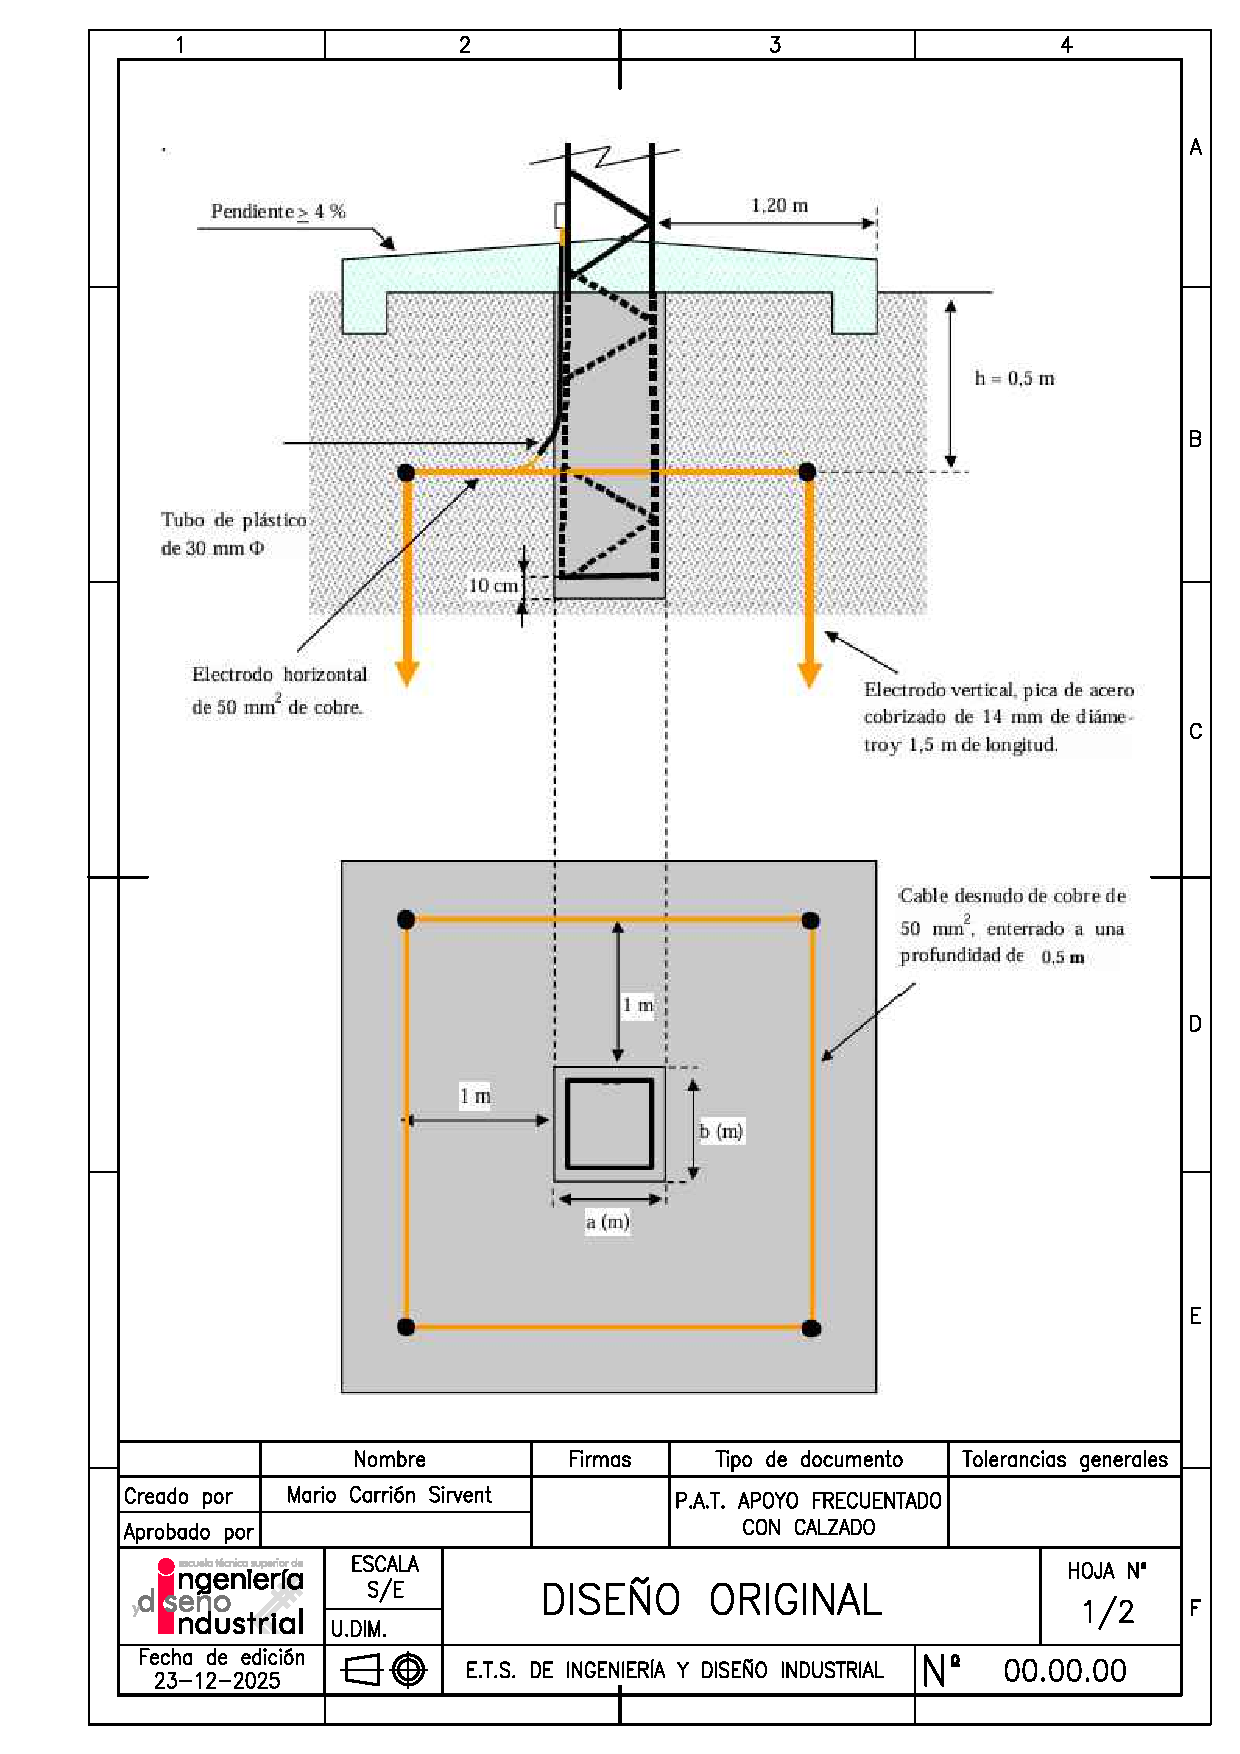
\includepdf[
  pages=-,          
  fitpaper=true,     
]{PDFs/pat-apoyoFC.pdf}

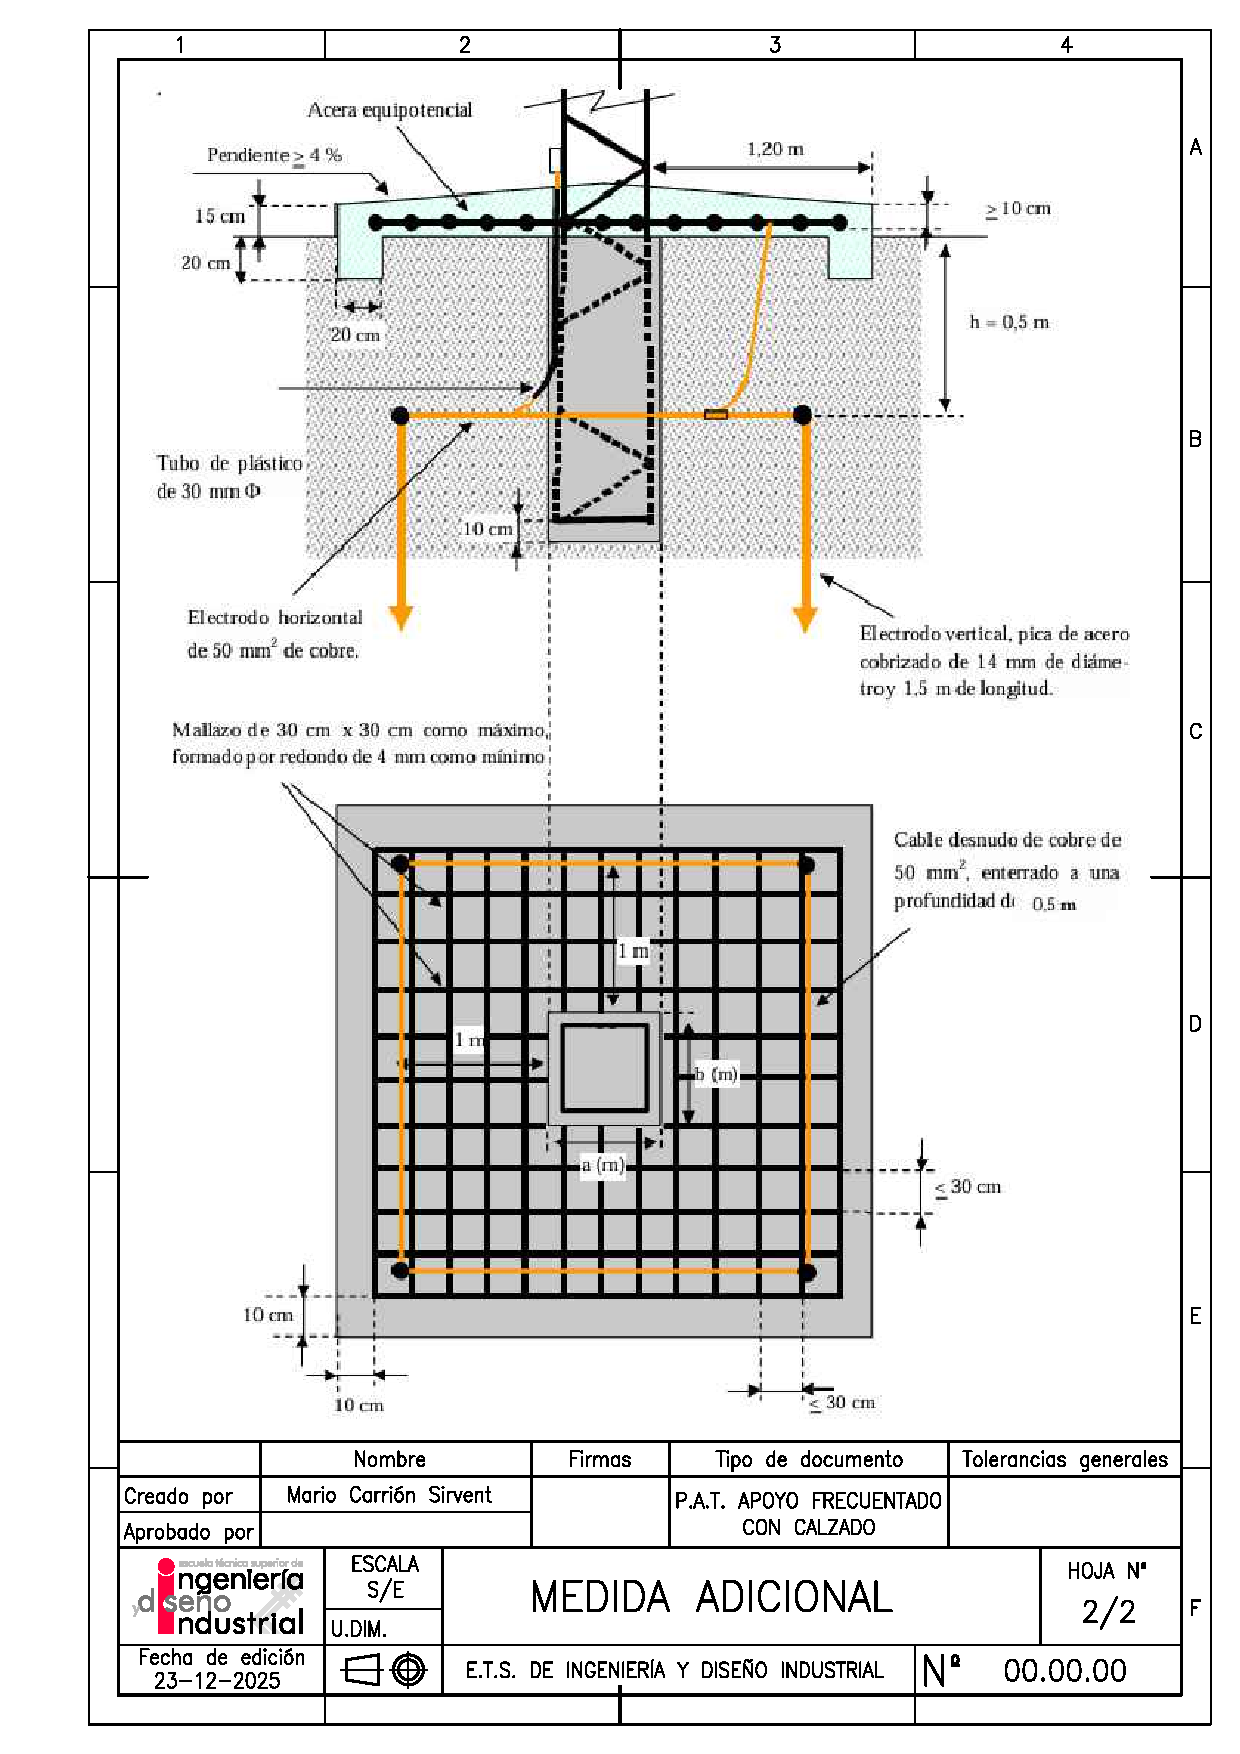
\includepdf[
  pages=-,          
  fitpaper=true,    
]{PDFs/pat-apoyoFCsol.pdf}
\chapter{Presupuesto}
\label{ch:presupuesto}
El presupuesto se ha obtenido a partir del programa IMEDEXSA. Ningún capítulo ni partida del presupuesto tiene en consideración el IVA.
\section{Presupuesto parcial}
\label{sec:presupuesto-parcial}
\subsection{Apoyos}
\label{subsec:presupuesto-parcialApoyos}
\begin{table}[H]
\caption{Presupuesto parcial de apoyos}
\centering
\begin{tabular}{|c|c|c|c|c|}
\hline
\rowcolor[HTML]{EFEFEF} 
\textbf{Nº Apoyo} & \textbf{Denominación} & \textbf{Armado} & \textbf{Peso (\si{\kilo\gram})} & \textbf{Importe (€)} \\ \hline
1                 & C-2000-22             & S1220           & 1069               & 2.138                  \\ \hline
2                 & C-500-22              & S1220           & 684                & 1.368                  \\ \hline
3                 & C-1000-22             & S1220           & 762                & 1.524                  \\ \hline
4                 & C-500-22              & S1220           & 684                & 1.368                  \\ \hline
5                 & C-500-22              & S1220           & 684                & 1.368                  \\ \hline
6                 & C-500-22              & S1220           & 684                & 1.368                  \\ \hline
7                 & C-500-24              & S1220           & 769                & 1.538                  \\ \hline
8                 & C-500-24              & S1220           & 769                & 1.538                  \\ \hline
9                 & C-500-14              & S1220           & 410                & 820                    \\ \hline
10                & C-500-16              & S1220           & 467                & 934                    \\ \hline
11                & C-500-18              & S1220           & 526                & 1.052                  \\ \hline
12                & C-500-20              & S1220           & 595                & 1.190                  \\ \hline
13                & C-500-22              & S1220           & 684                & 1.368                  \\ \hline
14                & C-500-22              & S1220           & 684                & 1.368                  \\ \hline
15                & C-500-22              & S1220           & 684                & 1.368                  \\ \hline
16                & C-500-14              & S1220           & 410                & 820                    \\ \hline
17                & C-500-22              & S1220           & 684                & 1.368                  \\ \hline
18                & C-500-24              & S1220           & 769                & 1.538                  \\ \hline
19                & C-500-20              & S1220           & 595                & 1.190                  \\ \hline
20                & C-500-20              & S1220           & 595                & 1.190                  \\ \hline
21                & C-500-16              & S1220           & 467                & 934                    \\ \hline
22                & C-500-18              & S1220           & 526                & 1.052                  \\ \hline
23                & C-2000-18             & S1220           & 844                & 1.688                  \\ \hline
\end{tabular}
\label{tab:presupuesto-parcialApoyos}
\end{table}
\textbf{TOTAL: \SI{30090}{€}.}
\subsection{Cimentaciones}
\label{subsec:presupuesto-parcialCim}
\begin{table}[H]
\caption{Presupuesto parcial de cimentaciones}
\centering
\label{tab:presupuesto-parcialCim}
\begin{tabular}{|c|c|c|c|}
\hline
\rowcolor[HTML]{EFEFEF} 
\textbf{Nº Apoyo} & \textbf{Tipo de cimentación} & \textbf{\begin{tabular}[c]{@{}c@{}}Volumen  \\ hormigón (\si{\cubic\meter})\end{tabular}} & \textbf{Importe (€)} \\ \hline
1                 & Monobloque                   & 4,44                                                                       & 280                  \\ \hline
2                 & Monobloque                   & 3,09                                                                       & 195                  \\ \hline
3                 & Monobloque                   & 3,5                                                                        & 220                  \\ \hline
4                 & Monobloque                   & 3,09                                                                       & 195                  \\ \hline
5                 & Monobloque                   & 3,09                                                                       & 195                  \\ \hline
6                 & Monobloque                   & 3,09                                                                       & 195                  \\ \hline
7                 & Monobloque                   & 3,52                                                                       & 222                  \\ \hline
8                 & Monobloque                   & 3,52                                                                       & 222                  \\ \hline
9                 & Monobloque                   & 1,72                                                                       & 108                  \\ \hline
10                & Monobloque                   & 2,02                                                                       & 127                  \\ \hline
11                & Monobloque                   & 2,35                                                                       & 148                  \\ \hline
12                & Monobloque                   & 2,65                                                                       & 167                  \\ \hline
13                & Monobloque                   & 3,09                                                                       & 195                  \\ \hline
14                & Monobloque                   & 3,09                                                                       & 195                  \\ \hline
15                & Monobloque                   & 3,09                                                                       & 195                  \\ \hline
16                & Monobloque                   & 1,72                                                                       & 108                  \\ \hline
17                & Monobloque                   & 3,09                                                                       & 195                  \\ \hline
18                & Monobloque                   & 3,52                                                                       & 222                  \\ \hline
19                & Monobloque                   & 2,65                                                                       & 167                  \\ \hline
20                & Monobloque                   & 2,65                                                                       & 167                  \\ \hline
21                & Monobloque                   & 2,02                                                                       & 127                  \\ \hline
22                & Monobloque                   & 2,35                                                                       & 148                  \\ \hline
23                & Monobloque                   & 3,39                                                                       & 214                  \\ \hline
\end{tabular}
\end{table}
\textbf{TOTAL: \SI{4205}{€}.}
\subsection{Conductores}
\label{subsec:presupuesto-parcialCond}
\begin{table}[H]
\caption{Presupuesto parcial de conductores}
\centering
\label{tab:presupuesto-parcialCond}
\begin{tabular}{|c|c|c|c|}
\hline
\rowcolor[HTML]{EFEFEF} 
\textbf{Conductor} & \textbf{Tipo} & \textbf{Longitud (Km)} & \textbf{Importe (€)} \\ \hline
Conductor de fase  & LA-56         & 12,11                  & 6.866                \\ \hline
\end{tabular}
\end{table}
\textbf{TOTAL: \SI{6866}{€}.}
\subsection{Aisladores}
\label{subsec:presupuesto-parcialAisl}
\begin{table}[H]
\caption{Presupuesto parcial de aisladores}
\centering
\label{tab:presupuesto-parcialAisl}
\begin{tabular}{|c|c|c|c|}
\hline
\rowcolor[HTML]{EFEFEF} 
\textbf{Elemento}          & \textbf{Tipo} & \textbf{Unidades (Ud.)} & \textbf{Importe (€)} \\ \hline
Aislador cadena amarre     & E-70P-127     & 90                      & 1.350                \\ \hline
Aislador cadena suspensión & E-70P-127     & 144                     & 2.160                \\ \hline
\end{tabular}
\end{table}
\textbf{TOTAL: \SI{3510}{€}.}
\subsection{Mano de Obra}
\label{subsec:presupuesto-parcialMO}
\begin{table}[H]
\caption{Presupuesto parcial de mano de obra}
\centering
\label{tab:presupuesto-parcialMO}
\begin{tabular}{|c|c|c|}
\hline
\rowcolor[HTML]{EFEFEF} 
\textbf{Elemento}                                                                             & \textbf{Unidades} & \textbf{Importe (€)} \\ \hline
Montaje, armado e izado de apoyos                                                             & 15.045 Kg.        & 13.540               \\ \hline
Excavación y hormigonado                                                                      & 67 m3             & 7.370                \\ \hline
\begin{tabular}[c]{@{}c@{}}Tendido, tensado y engrapado del conductor \\ de fase\end{tabular} & 12,11 Km.         & 73                   \\ \hline
\end{tabular}
\end{table}
\textbf{TOTAL: \SI{20983}{€}}
\section{Presupuesto total}
\label{sec:presupuesto-total}
\begin{table}[H]
\caption{Presupuesto total}
\centering
\label{tab:presupuesto-total}
\begin{tabular}{|c|c|c|c|c|}
\hline
\rowcolor[HTML]{EFEFEF} 
\textbf{DENOMINACIÓN}                                                                                       & \textbf{Ud.}                                              & \textbf{\begin{tabular}[c]{@{}c@{}}PRECIO \\ UNITARIO (€ )\end{tabular}} & \textbf{CANTIDAD} & \textbf{IMPORTE (€)} \\ \hline
Apoyos                                                                                                      & €/Kg.                                                     & 2                                                                        & 15.045            & 30.090               \\ \hline
Hormigón HM\_20                                                                                             & \begin{tabular}[c]{@{}c@{}}€/metro \\ cúbico\end{tabular} & 63                                                                       & 67                & 4.221                \\ \hline
\begin{tabular}[c]{@{}c@{}}Conductor fase LA-56\\ propio\end{tabular}                                       & Km.                                                       & 567                                                                      & 12,11             & 6.866                \\ \hline
Aislador E-70P-127                                                                                          & €/Ud.                                                     & 15                                                                       & 234               & 3.510                \\ \hline
\begin{tabular}[c]{@{}c@{}}Mano de obra Montaje,\\ armado e izado de\\ apoyos\end{tabular}                  & €/Kg.                                                     & 0,9                                                                      & 15045             & 13.540               \\ \hline
\begin{tabular}[c]{@{}c@{}}Mano de obra\\ Movimiento de tierra,\\ excavación y\\ hormigonado\end{tabular}   & €/m3.                                                     & 110                                                                      & 67                & 7.370                \\ \hline
\begin{tabular}[c]{@{}c@{}}Mano de obra Tendido,\\ tensado y engrapado del\\ conductor de fase\end{tabular} & €/Km.                                                     & 6                                                                        & 12,11             & 73                   \\ \hline
\end{tabular}
\end{table}

\textit{Presupuesto de ejecución material: \SI{65670}{€}.}

\textit{IVA: \SI{0}{\percent}.}

\textbf{TOTAL: \SI{65670}{€}.}

\chapter{Pliego de condiciones}
\label{ch:pliego}
\section{Objetivo}
\label{sec:pliego-objetivo}
Este Pliego de Condiciones determina los requisitos a que se debe  ajustar la ejecución de las instalaciones para la distribución de energía eléctrica, cuyas características técnicas estarán especificadas en el presente pliego y correspondiente proyecto.
\section{Disposiciones generales}
\label{sec:pliego-disposiciones}
La obra deberá ajustarse a la descripción realizada en la Memoria, Planos y Presupuesto del presente proyecto.

Las calidades de los materiales deberán respetar las especificaciones mínimas.

El director técnico de la obra será la única persona capacitada para juzgar, en caso de duda y omisiones del proyecto. Lo mismo que en caso de variación de parte o del total de la obra, si no estuviese bien realizada.

El contratista está obligado al cumplimiento de la reglamentación del trabajo correspondiente, la contratación del seguro obligatorio, subsidio familiar y de vejez, seguro de enfermedad y todas aquellas reglamentaciones de carácter social vigentes o que en lo sucesivo se dicten.  

En particular deberá cumplir lo dispuesto en la norma UNE 24042 Contratación de Obras, Condiciones Generales, siempre que no modifiquen el presente Pliego de Condiciones.  

El contratista deberá estar clasificado, según Orden del Ministerio de Hacienda de 28 de Marzo de 1968 en el grupo, subgrupo y categoría correspondientes al proyecto y que se fijará en el Pliego de Condiciones Particulares, en caso de que proceda.
\section{Organización del trabajo}
\label{sec:pliego-organizacion}
El Contratista ordenará los trabajos en la forma más eficaz para la perfecta ejecución de los mismos y las obras se realizarán siempre siguiendo las indicaciones del Director de Obra, al amparo de las condiciones siguientes:
\subsection{Datos de la obra}
\label{subsec:pliego-datosOrg}
Se entregará al Contratista una copia de los planos y Pliego de Condiciones del Proyecto, así como cuantos planos o datos necesite para la completa ejecución de la Obra.

El Contratista podrá tomar nota o sacar copia a su costa de la Memoria, Presupuesto y Anexos del Proyecto, así como segundas copias de todos los documentos.

El Contratista se hace responsable de la buena conservación de los originales de donde  obtenga las copias, los cuales serán devueltos al Director de Obra después de su utilización.  

Por otra parte, en un plazo máximo de dos meses, después de la terminación de los trabajos, el Contratista deberá actualizar los diversos planos y documentos existentes, de acuerdo con las características de la Obra terminada, entregando al Director de Obra dos expedientes  completos relativos a los trabajos realmente ejecutados.  

No se harán por el Contratista alteraciones, correciones, ni adiciones o variaciones sustanciales en los datos fijados en el Proyecto, salvo aprobación previa por escrito del Director de Obra.
\subsection{Replanteo de la obra}
\label{subsec:pliego-replanteoOrg}
El Director de Obra, una vez que el Contratista esté en posesión del Proyecto y antes de comenzar las obras, deberá hacer el replanteo de las mismas, con especial atención a los puntos singulares, entregando al Contratista las referencias y datos necesarios para fijar completamente  la ubicación de las mismas.  

Se levantará por duplicado un Acta, en la que constarán, muy bien los datos entregados,  firmados por el Director de Obra y por el representante del Contratista.  

Los gastos de replanteo serán por cuenta del Contratista.   
\subsection{Mejoras y variaciones del proyecto}
\label{subsec:pliego-mejorasOrg}
No se considerarán como mejoras ni variaciones del Proyecto más que aquellas que hayan sido ordenadas expresamente por escrito,por el Director de Obra y convenido precio antes de proceder a su ejecución.  

Las obras accesorias o delicadas,  no incluidas en los precios de adjudicación,  podrán ejecutarse con personal independiente del Contratista.
\subsection{Recepción del material}
\label{subsec:pliego-recepcionOrg}
El Director de Obra, de acuerdo con el Contratista, dará a su debido tiempo su aprobación sobre el material suministrado y confirmará que permite una instalación correcta.

La vigilancia y conservación del material suministrado será por cuenta del Contratista. 
\subsection{Organización}
\label{subsec:pliego-organizacionnOrg}
El Contratista actuará de patrono legal, aceptando todas las responsabilidades correspondientes y quedando obligado al pago de los salarios y cargas que legalmente están establecidas, y en general, a todo cuanto se legisle, decrete  u ordene sobre el particular antes o durante la ejecución de la obra.

Dentro de lo estipulado en el Pliego de Condiciones, la organización de la Obra, así como la determinación de la procedencia de los materiales que se empleen, estará a cargo del Contratista a quien corresponderá la responsabilidad de la seguridad contra accidentes.  

El Contratista deberá, sin embargo, informar al Director de Obra de todos los planes de organización técnica de la Obra, así como de la procedencia de los materiales y cumplimentar  cuantas ordenes le dé éste en relación con datos extremos.  
En las obras por administración, el Contratista deberá dar cuenta diaria al Director de Obra de la admisión de personal, compra de materiales, adquisición o alquiler de elementos auxiliares y cuantos gastos haya de efectuar. 

Para los contratos de trabajo, compra de material o alquiler de elementos auxiliares, cuyos salarios, precios o cuotas sobrepasen en más de un \SI{5}{\percent} de los normales en el mercado, solicitará la aprobación previa del Director de Obra, quien deberá responder dentro de los ocho días siguientes a la petición, salvo casos de reconocida urgencia, en los que se dará cuenta posteriormente. 

\subsection{Ejecución de las obras}
\label{subsec:pliego-ejecucionOrg}
Las obras se ejecutarán conforme al Proyecto y a las condiciones contenidas en éste Pliego de condiciones y en el Pliego Particular si lo hubiera, y de acuerdo con las especificaciones señaladas en el de Condiciones Técnicas.  

El Contratista, salvo aprobación por escrito del Director de Obra, no podrá hacer ninguna alteración o modificación de cualquier naturaleza tanto en la ejecución de la obra en relación con el Proyecto, como en las Condiciones Técnicas especificadas.

El Contratista no podrá utilizar, en los trabajos, personal que no sea de su exclusiva cuenta y cargo.

Igualmente será de su exclusiva cuenta y cargo aquel personal ajeno al propiamente manual y que sea necesario para el control administratívo del mismo.

El Contratista deberá tener al frente de los trabajos un técnico suficientemente especializado a juicio del Director de Obra.
\subsection{Subcontratación de las obras}
\label{subsec:pliego-subcontrataOrg}
Salvo que el contrato disponga lo contrario o que de su naturaleza y condiciones se deduzca que la Obra ha de ser ejecutada directamente por el adjudicatario, podrá éste concertar con terceros la realización de determinadas unidades de obra.  

La celebración de los subcontratos estará sometida al cumplimiento de los siguientes requisitos:
\begin{enumerate}[label=\alph*)]
  \item A que se de conocimiento por escrito al Director de Obra del subcontrato a celebrar, con indicación de las partes de obra a realizar y sus condiciones económicas, a fin de que aquel lo autorice previamente.  
  \item A que las unidades de obra que el adjudicatario contrate con terceros no exceda del \SI{50}{\percent} del presupuesto total de la obra principal.
\end{enumerate}
En cualquier caso el Contratante no quedará vinculado en absoluto ni reconocerá ninguna obligación contractual entre él y el subcontratista y cualquier subcontratación de obras no eximirá al Contratista de ninguna de sus obligaciones con respecto al Contratante.  
\subsection{Plazo de ejecución}
\label{subsec:pliego-plazoejecucionOrg}
Los plazos de ejecucion, total y parciales, indicados en el contrato, se empezarán a contar a partir de la fecha de replanteo.  
El Contratista estará obligado a cumplir con los plazos que se señalen en el contrato para la ejecución de las obras y que serán improrrogables.   

No obstante lo anteriormente indicado, los plazos podrán ser objeto de modificaciones cuando así resulte por cambios determinados por el Director de Obra debidos a exigencias de la realización de las obras y siempre que tales cambios influyan realmente en los plazos señalados en el contrato.   

Si por cualquier causa, ajena por completo al Contratista, no fuera posible empezar los trabajos en la fecha prevista o tuvieran que ser suspendidos una  vez empezados, se concederá por el Director de Obra, la prorroga estrictamente necesaria.  
\subsection{Recepción provisional}
\label{subsec:pliego-recepcionprovisionalOrg}
Una vez terminadas las obras y a los quince días siguientes a la petición del Contratista se hará la recepción provisional de las mismas por el Contratante, requiriendo para ello la presencia del Director de Obra y del representante del Contratista levantandose las Actas que correspondan en las que se harán constar la conformidad con los trabajos realizados, si éste es el caso.

Dichas Actas serán firmadas por el Director de Obra y el representante del Contratista, dándose la Obra por recibida si se ha ejecutado correctamente de acuerdo con las especificaciones dadas en el Pliego de Condiciones Técnicas y en el Proyecto correspondiente, comenzandose entonces a contar el plazo de garantía.

En el caso de no hallarse la Obra en estado de ser recibidad,  se hará constar  así en el Acta y  se darán al Contratista las instrucciones precisas y detalladas para remediar los defectos observados, fijandose un plazo de ejecución.

Expirado dicho plazo, se hará un nuevo reconocimiento.  Las obras de reparación  serán por cuenta y a cargo del Contratista.  
Si el Contratista no cumpliese estas prescripciones podrá declararse rescindido  el contrato con pérdida de la fianza.  
\subsection{Períodos de garantía}
\label{subsec:pliego-garantiaOrg}
El periodo de garantía será señalado en el contrato y empezará a contar desde la fecha de aprobación del Acta de Recepción. 

Hasta que tenga lugar la recepción definitiva, el Contratista es responsable de la conservación de la Obra, siendo de su cuenta y cargo las reparaciones por defectos de ejecución o mala calidad de los materiales.

Durante  este periodo, el Contratista garantizará al Contratante contra toda  reclamación de terceros, fundada en causa y por ocasión de la ejecución de la Obra.
\subsection{Recepción definitiva}
\label{subsec:pliego-recepciondefOrg}
Al terminar el Plazo de garantía señalado en el contrato o en su defecto a los  seis meses de la recepción provisional, se procedera a la recepción definitiva  de las obras, con la concurrencia del Director de Obra y del representante del Contratista levantándose el Acta correspondiente, por duplicado (si las obras son conformes), que quedará firmada por el Director de Obra y el representante  del Contratista y ratificada por el Contratante y el Contratista.
\subsection{Pago de obras}
\label{subsec:pliego-pagoOrg}
El pago de las obras realizadas se hará sobre certificaciones parciales, que se practicarán mensualmente. Dichas certificaciones contendrán solamente las unidades de obra totalmente terminadas que se hubieran ejecutado en el plazo a que se refieran.  

La relación valorada que figure en las certificaciones, se hará con arreglo a los precios establecidos, y con la ubicación, planos y referencias necesarias para su comprobación.

El Director de Obra expedirá las Certificaciones de las obras ejecutadas que tendrán carácter de documento provisional a buena cuenta, rectificables por la  liquidación definitiva o por las certificaciones siguientes.
\subsection{Abono de materiales acopiados}
\label{subsec:pliego-abonomatOrg}
Cuando a juicio del Director de Obra no haya peligro de que desaparezcan o se  deterioren los materiales acopiados y reconocidos como útiles, se abonarán con arreglo a los precios descompuestos de la adjudicación. 

Dicho material será indicado por el Director de Obra e indicado en el Acta de recepción de Obra.  

La restitución de las bobinas vacías se hará en el plazo de un mes, una vez que  se haya instalado el cable que contenían.  
\section{Condiciones técnicas de la ejecución}
\label{sec:pliego-condiciones}
\subsection{Excavaciones}
\label{subsec:pliego-excavacionesCT}
Las dimensiones de las excavaciones se ajustarán lo más posible a las dadas en el Proyecto o en su defecto a las indicadas por el Director de Obra.  

Las paredes de los hoyos serán verticales. Cuando sea necesario variar el volumen de la excavación, se hará de acuerdo con el Director de Obra.  

El Contratista tomara las disposiciones convenientes para dejar el menor tiempo posible abiertas las excavaciones, con objeto de evitar accidentes. Las excavaciones se realizarán con útiles apropiados según el tipo de terreno.   

En terrenos rocosos será imprescindible el uso de explosivos o martillo compresor, siendo por cuenta del Contratista la obtención de los permisos de  utilización de explosivos.  

Cuando deban emplearse explosivos, el Contratista deberá tomar las precauciones adecuadas para que en el momento de la explosión no se proyecten al exterior piedras que puedan provocar accidentes o desperfectos, cuya responsabilidad correría a cargo del Contratista.

En terrenos con agua deberá procederse a su desecado, procurando hormigonar después lo más rapidamente posible para evitar el riesgo de desprendimientos en las paredes del hoyo, aumentando así las dimensiones del mismo.

\subsection{Hormigonado}
\label{subsec:pliego-hormigonadoCT}
Este se deberá dosificar a \SI{250}{\kilo\gram} de cemento por cada metro cúbico.

Si la excavación superara el \SI{10}{\percent} del volumen técnico, por conveniencia del contratista, siempre de acuerdo con el Director técnico de las obras, o el empleo de explosivos, la dosificación del hormigón será siempre la misma.

El cemento empleado será Portland, de fraguado lento, o bien de otra marca similar, de primera calidad.
    
Los áridos empleados para las cimentaciones de los apoyos, deberán ser de buena calidad, limpios y no heladizos, estando exentos de materiales orgánicos y de arcillas.

Será preferible la piedra con aristas y superficies rugosas y ásperas, por su mayor adherencia al mortero.

La arena puede proceder de minas o canteras, ríos, o bien, de machaqueo.

La dimensión de los granos de arena no será superior al \SI{6}{\percent} (ensayo de granulometría).

El agua empleada para la ejecución del hormigón será limpia y exenta de elementos orgánicos, arcillas, etc.
\subsection{Armado e izado de los apoyos metálicos}
\label{subsec:pliego-izadoCT}
El transporte de todos los materiales a la obra se realizará con el mayor cuidado, e intentando evitar al máximo los posibles desperfectos que pudieran acontecer.

En caso de dobleces de barras, éstas se enderezarán en caliente. Los taladros que se tengan que realizar, se harán con punzón o carraca, nunca por sopletes. Los taladros que no se usen, se cerrarán por medio de soldadura. En caso de que haya que aumentar el diámetro de los mismos, se hará por mediación del escariador. Se deberán eliminar las rebabas de los mismos.

Para el armado se empleará puntero y martillo para que coincidan las piezas que se unen, pero con cuidado para no agrandar el taladro.
Se aconseja armar en tierra el mayor número posible de piezas.

El izado deberá hacerse sin originar deformaciones permanentes sobre elementos que componen el apoyo.
Cuando la torre está izada, se hará un repaso general del ajuste de los componentes.

Los postes de hormigón se transportarán en vehículos preparados al efecto, y, al depositarlos se hará en un lugar llano y con sumo cuidado en evitación de deformaciones de los mismos.

Todas las piezas deberán estar recubiertas de material blando y flexible (gomas naturales o sintéticas).
\subsection{Tendido, tensado y regulado de los conductores}
\label{subsec:pliego-tendidoCT}
Los cables deberán tratarse con el mayor cuidado para evitar deterioros, lo mismo que las bobinas donde se transportan.

En la hora de desenrollar los cables se debe cuidar que no rocen con el suelo.

Para ejercer la tracción se pueden emplear cuerdas pilotos, pero deben ser las mismas del tipo flexible y antigiratorias, montando bulones de rotación para compensar los defectos de la torsión. Si se produce alguna rotura en los hilos de los cables, por cualquier causa, se deberán colocar manguitos separatorios.
	
Todo el tendido y tensado de los conductores se realizará conforme a la tabla de tendido proporcionada por el proyectista, y conforme a las características climatológicas a las que se va a realizar la operación.
\begin{itemize}
    \item \textbf{Poleas de tendido:} Para cables de aluminio, éstas serán de aleación de aluminio. El diámetro será entre 25 y 30 veces el diámetro del cable que se extienda. Esta polea estará calculada para aguantar esfuerzos a que deba ser sometida.
    \item \textbf{Tensado:} Este deberá realizarse arriostrando las torres de amarre a los apoyos de hormigón de anclajes en sentido longitudinal. El tensado de los cables se hará por medio de un cable piloto de acero en evitación de flexiones exageradas. Todos los aparatos para el tensado deberán colocarse a distancia conveniente de la torre de tense, para que el ánguo formado por las tangentes del piloto al paso por la polea no sea inferior a os 150 grados.
    \item \textbf{Regulado:} Toda línea se divide en trozos de longitudes varialbles según situación de vértices. En el perfil longitudinal se definen los vanos y en los cálculos las flechas de cada uno de ellos, y al mismo se deberá adaptar.
\end{itemize}
\subsection{Cadena de aisladores}
\label{subsec:pliego-aislCT}
Estos se limpiarán cuidadosamente antes de ser montados. Se tendrá especial cuidado en su traslado y colocación para que no sufran desperfectos los herrajes que unen las cadenas.
\subsection{Empalmes}
\label{subsec:pliego-empalmesCT}
Serán de tal calidad que garanticen la resistencia mecánica exigida por los Reglamentos y no exista aumento de la resistencia del conductor.

Los empalmes deberán ser cepillados cuidadosamente, tanto interior como exteriormente, con cepillo y baquetas especiales.
\subsection{Engrapado}
\label{subsec:pliego-engrapadoCT}
Para el mismo se deberá tomar medida para conseguir un buen aplomo de las cadenas de aisladores.
	
El apretado de los tornillos de las grapas se debe hacer alternativamente para asegurar un buen apriete.
\section{Características de los materiales}
\label{sec:pliego-materiales}
Todos los materiales serán de primera calidad. No deberán presentar deterioro ni defecto alguno que disminuya la función que tengan que desarrollar.
\subsection{Conductores trenzados}
\label{subsec:pliego-trenzadosMAT}
Deberán ir provistos de cubierta de aislamiento, el cual será de polietileno reticulado (PRC).

Se deberán distinguir de otros por lo que deberán ir grabados en tintas blancas o relieves en el exterior.

Las secciones de los conductores serán las determinadas en la Memoria.

Los empalmes deberán realizarse mediante manguitos a compresión y el aislamiento será regenerado con cinta de goma autovulcanizante y recubierta con cinta de P.V.C.
\subsection{Conductores de cobre}
\label{subsec:pliego-cobreMAT}
Estos estarán formados, según la sección, por uno o por varios alambres de cobre, cilíndricos, de buena calidad y resistencia mecánica y libres de todos los desperfectos posibles, así como de imperfecciones.
\subsection{Abrazaderas y tacos de sujeción}
\label{subsec:pliego-abrazaderasMAT}
Las abrazaderas serán de placas de acero isoplastificados y de una sola pieza, dotadas de punta de acero roscada.

Las abrazaderas para cable fiador, serán las mismas, de iguales características, pero sin punta de acero.
\subsection{Herrajes}
\label{subsec:pliego-herrajesMAT}
El cable fiador de acero y de arriostramiento será flexible y galvanizado.

El resto de los herrajes (aprietahilos, grilletes, etc.), serán galvanizados en caliente.
\subsection{Torres metálicas}
\label{subsec:pliego-torresMAT}
Serán de hierro laminado y responderán a la altura determinada en la Memoria.

Serán galvanizadas en caliente. Las cimentaciones se tendrán que adaptar a lo especificado en el cálculo de las mismas.



\chapter{Estudio de Seguridad y Salud}
\label{ch:sys}
\section{Objetivo}
\label{sec:sys-objetivo}
El objeto del presente Estudio de Seguridad y Salud es la redacción de los documentos necesarios que definan, en el marco del Real Decreto 1627/1997, de 24 de Octubre, por el que se establecen disposiciones mínimas de seguridad y salud en las obras de construcción, las previsiones y desarrollo de las soluciones necesarias para los problemas de ejecución de la obra, y la prevención de riesgos de accidentes preceptivas de sanidad, higiene y bienestar de los trabajadores durante el desarrollo de la misma.
	
En aplicación de este Estudio de Seguridad y Salud de la obra, cada contratista, subcontratista y trabajadores autónomos, elaborarán un plan de seguridad y salud en el trabajo, en el que se analicen , estudien, desarrollen y complementen las previsiones contenidas en este estudio.
\section{Datos generales de la obra}
\label{sec:sys-obra}
El presente Estudio Básico de Seguridad y Salud se refiere al Proyecto de la línea aérea de alta tensión, cuyos datos generales son:
\begin{itemize}[label=--]
    \item \textit{Proyecto de Ejecución:} Línea de A.T. L'Albir-Benidorm.
    \item \textit{Autor del Proyecto:} Mario Carrión Sirvent
    \item \textit{Emplazamiento:} Alicante
    \item \textit{Presupuesto de Ejecución material:} \SI{65670}{€}.
\end{itemize}
Las unidades constructivas que componen la presente obra son:
\begin{itemize}
    \item Replanteo.
    \item Desbroce.
    \item Excavación.
    \item Cimentación.
    \item Armado e izado de apoyos.
    \item Instalación de conductores desnudos.
    \item Instalación de aisladores
    \item Instalación de crucetas.
    \item Instalación de aparatos de seccionamiento y corte (interruptores, seccionadores, fusibles...).
    \item Instalación de limitadores de sobretensión (autoválvulas).
    \item Instalación de transformadores tipo intemperie sobre apoyos.
    \item Instalación de dispositivos antivibraciones.
    \item Medida de altura de conductores.
    \item Detección de partes en tensión.
    \item Interconexión entre elementos.
    \item Conexión y desconexión de líneas o equipos.
    \item Puesta a tierra y conexiones equipotenciales.
\end{itemize}
\section{Normativa aplicable}
\label{sec:sys-normativa}
\subsection{Normas oficiales}
\label{subsec:sys-normasOficiales}
Son de obligado cumplimiento todas las disposiciones legales o reglamentarias, resoluciones y cuantas otras fuentes normativas contengan concretas regulaciones en materia de Seguridad e Higiene en el trabajo, propias de la Industria Eléctrica o de carácter general, que se encuentren vigentes y sean de aplicación durante el tiempo en el que subsista la relación contractual promotor-contratista, según las actividades a realizar.

En particular:
\begin{itemize}
    \item Ley 8/1980, de 1 de marzo, del Estatuto de los Trabajadores
    \item Ordenanza General de Seguridad e Higiene en el Trabajo (9 de marzo de 1971).
    \item Homologación de medios de Protección personal de los trabajadores (BOL. de 29 de mayo de 1974. Orden de 15 de julio de 1974).
    \item Estatuto de los Trabajadores (Ley 8/1980, de 20 de marzo).
    \item Ley de Prevención de Riesgos Laborales (Ley 31/1995, de 8 de noviembre).
    \item Real Decreto 39/1997, de 17 de enero, por el que se aprueba el Reglamento de los Servicios de Prevención.
    \item Orden de 27 de junio de 1997, por la que se desarrolla el RD 39/1.997, de 17 de enero.
    \item Real Decreto 485/1997, de 14 de abril, sobre disposiciones mininas en materia de señalización de seguridad y salud en el trabajo.
    \item Real Decreto 486/1997, de 14 de abril, por el que se establecen disposiciones mínimas de seguridad y salud en los lugares de trabajo.
    \item Real Decreto 487/1997, de 14 de abril, sobre disposiciones mínimas de seguridad y salud relativas a la manipulación manual de cargas que entrañen riesgos, en particular dorso-lumbares, para los trabajadores.
    \item  Real Decreto 773/1997, de 30 de mayo, sobre disposiciones mínimas de seguridad y salud relativas a la utilización por los trabajadores de equipos de protección individual.
    \item Real Decreto 949/1997, de 20 de Junio, por el que se establece el certificado de profesionalidad de la ocupación de prevencionista de riesgos laborales. 
    \item Real Decreto 1215/1997, de 18 de julio, por el que se establecen las disposiciones mínimas de seguridad y salud para la utilización por los trabajadores de los equipos de trabajo.
    \item Real Decreto 1627/1997, de 24 de octubre, por el que se establecen disposiciones mínimas de seguridad y de salud en las obras de construcción.
    \item Real Decreto 223/2008 de 15 de febrero, por el que se aprueban el Reglamento sobre condiciones técnicas y garantías de seguridad en líneas eléctricas de alta tensión y sus instrucciones técnicas complementarias ITC-LAT 01 a 09.
    \item Reglamento sobre Condiciones Técnicas y de Garantía de Seguridad en Centrales Eléctricas, Subestaciones y Centros de transformación (Decreto 3275/1982 de 12 de noviembre) e instrucciones Técnicas Complementarias.
\end{itemize}
\subsection{Normas específicas}
\label{subsec:sys-normasEspecificas}
Dentro de estas Normas deben tener especialmente en cuenta todas las Recomendaciones, Prescripciones e Instrucciones de la Asociación de Medicina y Seguridad en el Trabajo de UNESA para la Industria Eléctrica (AMYS), que se recogen en:
\begin{itemize}
\item “Prescripciones de Seguridad para trabajos y maniobras en instalaciones eléctricas”.
\item “Prescripciones de Seguridad para trabajos mecánicos y diversos”.
\item Instrucción General para la realización de los trabajos en tensión en Alta Tensión y sus Desarrollos.
\item Instrucción General para la realización de los trabajos en tensión en Baja Tensión y sus Desarrollos.
\end{itemize}
\section{Obligación del promotor}
\label{sec:sys-promotor}
El promotor está obligado a incluir el presente Estudio de Seguridad y Salud, como documento del Proyecto de Obra.

Antes del inicio de los trabajos, designará un coordinador en materia de seguridad y salud, cuando en la ejecución de las obras intervengan más de una empresa, o empresas y trabajadores autónomos, o diversos trabajadores autónomos.

La designación de coordinadores en materia de seguridad y salud no eximirá al promotor de sus responsabilidades.

El promotor deberá efectuar un aviso a la autoridad laboral competente antes del comienzo de las obras, que se redactará con arreglo a lo dispuesto en el Anexo III del R.D. 1627/1997, de 24 de octubre, debiendo exponerse en la obra de forma visible y actualizándose si fuera necesario.
\section{El coordinador}
\label{sec:sys-coordinador}
El Coordinador en materia de seguridad y salud durante la ejecución de la obra, deberá coordinar los principios generales de prevención y de seguridad, tomando las decisiones técnicas y de organización con el fin de planificar los distintos trabajos o fases que vayan a desarrollarse simultánea o sucesivamente.
	
Deberá coordinar las actividades de la obra para garantizar que los contratistas y, en su caso, los subcontratistas y los trabajadores autónomos, apliquen de manera coherente y responsable los principios de la acción preventiva que se recogen en el artículo 15 de la Ley de prevención de Riesgos Laborales durante la ejecución de la obra y, en particular, en las tareas o actividades a que se refiere el artículo 10 del Decreto 1627/1997 de 24 de octubre, sobre disposiciones mínimas de seguridad y de salud en las obras de construcción.
	
El Coordinador deberá aprobar el Plan de Seguridad y Salud elaborado por el contratista y, en su caso, las modificaciones introducidas en el mismo.

Así mismo organizará la coordinación de actividades empresariales previstas en el artículo 24 de la Ley de Prevención de Riesgos Laborales y coordinará las acciones y funciones de control de la aplicación correcta de los métodos de trabajo.

El Coordinador deberá adoptar las medidas necesarias para que sólo las personas autorizadas puedan acceder a la obra.
\section{Contratistas y subcontratistas}
\label{sec:sys-contratistas}
Estarán obligados a aplicar los principios de la acción preventiva que se recogen en el artículo 15 de la Ley de Prevención de Riesgos Laborales, cumplir y hacer cumplir a su personal lo establecido en el Plan de Seguridad y Salud e informar y proporcionar las instrucciones adecuadas a los trabajadores autónomos sobre todas las medidas que hayan de adoptarse en lo que se refiere a seguridad y salud en la obra.

Deberán atender las indicaciones y cumplir las instrucciones del coordinador en materia de seguridad y salud durante la ejecución de la obra.

Los contratistas y subcontratistas serán responsables de la ejecución correcta de las medidas preventivas fijadas en el plan de seguridad y salud en lo relativo a las obligaciones que les correspondan a ellos directamente o, en su caso, a los trabajadores autónomos por ellos contratados.

Además los contratistas y subcontratistas responderán solidariamente de las consecuencias que se deriven del incumplimiento de las medidas previstas en el plan en los términos del apartado 2 del artículo 42 de la Ley de Prevención de Riesgos Laborales.

Las responsabilidades de los coordinadores, de la dirección facultativa y del promotor no eximirán de sus responsabilidades a los contratistas y a los subcontratistas.

Los equipos de protección individual a disponer para cada uno de los puestos de trabajo a desempeñar, determinadas en el Plan de Seguridad y Salud en el Trabajo a elaborar por el contratista, estarán en consonancia con el resultado previsto por éste en la evaluación de los riesgos que está obligado a realizar en cumplimiento del R.D. 39/1.997, de 17 de Enero, por el que se aprueba el Reglamento de los Servicios de Prevención. Una copia de dicha evaluación y de su resultado, se adjuntará al Plan en el momento de su presentación.

Asimismo, y en aplicación del R.D. 773/1.997, de 30 de Mayo, sobre disposiciones mínimas de seguridad y salud relativas a la utilización por los trabajadores de los equipos de protección individual, es responsabilidad del contratista suministrar dichas protecciones individuales a los trabajadores de manera gratuita, reponiéndolas cuando resulte necesario, motivo por el cual, dentro del Plan de Seguridad y Salud en el Trabajo a elaborar por el contratista, éstas se relacionarán exhaustivamente en todos los apartados del mismo, de acuerdo con lo señalado en el párrafo anterior, pero no se valorarán dentro del presupuesto del plan.
\section{Obligaciones de los trabajadores}
\label{sec:sys-obligaciones}
Los trabajadores están obligados a:
\begin{enumerate}
    \item Aplicar los principios de la acción preventiva que se recoge en el artículo 15 de la Ley de Prevención de Riesgos Laborales, y en particular:
    \begin{itemize}[label=--]
        \item Mantenimiento de la obra en buen estado de orden y limpieza.
        \item Almacenamiento y evacuación de residuos y escombros.
        \item Recogida de materiales peligrosos utilizados.
        \item Adaptación del periodo de tiempo efectivo que habrá de dedicarse a los distintos trabajos o fases de trabajo.
        \item Cooperación entre todos los intervinientes en la obra.
        \item Interacciones o incompatibilidades con cualquier otro trabajo o actividad.
    \end{itemize}
  \item Cumplir las disposiciones mínimas establecidas en el Anexo IV del R.D. 1627/1997.
  \item Ajustar su actuación conforme a los deberes sobre coordinación de las actividades empresariales previstas en le artículo 24 de la Ley de Prevención de Riesgos Laborales, participando en particular en cualquier medida de actuación coordinada que se hubiera establecido.
  \item Cumplir con las obligaciones establecidas para los trabajadores en el artículo 29, apartados 1 y 2 de la Ley de Prevención de Riesgos Laborales.
  \item Utilizar equipos de trabajo que se ajusten a lo dispuesto en el R.D. 1215/1997.
  \item Elegir y utilizar equipos de protección individual en los términos previstos en el R.D. 773/1997.
  \item Atender las indicaciones y cumplir las instrucciones del coordinador en materia de seguridad y salud.
\end{enumerate}
Los trabajadores autónomos deberán cumplir lo establecido en el plan de seguridad y salud.
\section{Libro de incidencias}
\label{sec:sys-incidencias}
En cada centro de trabajo existirá, con fines de control y seguimiento del plan de seguridad y salud, un libro de incidencias que constará de hojas duplicadas y que será facilitado por el colegio profesional al que pertenezca el técnico que haya aprobado el plan de seguridad y salud.

Deberá mantenerse siempre en obra y en poder del coordinador. Tendrán acceso al libro, la Dirección Facultativa, los contratistas y subcontratistas, los trabajadores autónomos, las personas con responsabilidades en materia de prevención de las empresas intervinientes, los representantes de los trabajadores, y los técnicos especializados de las Administraciones Públicas competentes en esta materia, quienes podrán hacer anotaciones en el mismo.

Efectuada una anotación en el libro de incidencias, el coordinador estará obligado a remitir en el plazo de \SI{24}{\hour} una copia a la Inspección de Trabajo y Seguridad Social de la provincia en que se realiza la obra. Igualmente notificará dichas anotaciones al contratista y a los representantes de los trabajadores.
\section{Derecho de los trabajadores}
\label{sec:sys-derechos}
Los contratistas y subcontratistas deberán garantizar que los trabajadores reciban una información adecuada y comprensible de todas las medidas que hayan de adoptarse en lo que se refiere a seguridad y salud en la obra.

Una copia del plan de seguridad y salud y de sus posibles modificaciones, a los efectos de su conocimiento y seguimiento, será facilitada por el contratista a los representantes de los trabajadores en el centro de trabajo.
\section{Prevención de riesgos profesionales}
\label{sec:sys-prl}
\subsection{Protecciones individuales generales}
\label{subsec:sys-prlEPI}
\begin{enumerate}
    \item Cascos: para todas las personas que participan en obra, incluidos visitantes.
    \item Guantes de uso general.
    \item Guantes de goma.
    \item Guantes de soldador.
    \item Guantes diacetílicos.
    \item Botas de agua.
    \item Botas de seguridad de lona.
    \item Botas de seguridad de cuero.
    \item Botas dialécticas.
    \item Gafas de soldador.
    \item Gafas de seguridad antiproyecciones.
    \item Pantalla de soldador.
    \item Mascarillas antipolvo.
    \item Protectores auditivos.
    \item Polainas de soldador.
    \item Manguitos de soldador.
    \item Mandiles de soldador.
    \item Cinturón de seguridad de sujeción.
    \item Cinturón antivibratorio.
    \item Chalecos reflectantes.
\end{enumerate}
\subsection{Protecciones colectivas generales}
\label{subsec:sys-prlEPC}

\begin{enumerate}
    \item Pórticos protectores de líneas eléctricas.
    \item Vallas de limitación y protección.
    \item Señales de seguridad.
    \item Cintas de balizamiento.
    \item Redes.
    \item Soportes y anclajes de redes.
    \item Tubo sujeción cinturón de seguridad.
    \item Anclaje para tubo.
    \item Balizamiento luminoso.
    \item Extintores.
    \item Interruptores diferenciales
    \item Toma de tierra.
    \item Válvula antiretroceso.
    \item Riegos.
\end{enumerate}
\subsection{Formación}
\label{subsec:sys-prlFormacion}
Todo personal debe recibir, al ingresar en la obra, una exposición de los métodos de trabajo y los riesgos que éstos pudieran entrañar, juntamente con las medidas de seguridad que deberá emplear.

Eligiendo al personal más cualificado impartirán cursillos de socorrismo y primeros auxilios, de forma que todos los trabajos dispongan de algún socorrista.

Se informará a todo el personal interviniente en la obra, sobre la existencia de productos inflamables, tóxicos, etc. y medidas a tomar en cada caso.
\subsection{Medicina preventiva y primeros auxilios}
\label{subsec:sys-prlMedicina}
Se tendrán en cuenta las siguientes consideraciones:
\begin{enumerate}
    \item Botiquín: Deberá existir en la obra al menos un botiquín con todos los elementos suficientes para curas, primeros auxilios, dolores, etc.
    \item Asistencia a accidentados: Se deberá informar a la obra del emplazamiento de los diferentes Centros Médicos, Residencia Sanitaria, médicos, ATS., etc., donde deba trasladarse a los posibles accidentados para un más rápido y efectivo tratamiento, disponiendo en la obra de las direcciones, teléfonos, etc., en sitios visibles.
    \item Reconocimiento Médico: todo el personal que empiece a trabajar en la obra deberá pasar un reconocimiento médico previo que certifique su aptitud.
    \item Instalaciones: se dotará a la obra, si así se estima en el correspondiente Plan de Seguridad, de todas las instalaciones necesarias, tales como:
    \begin{itemize}[label=--]
        \item Almacenes y talleres:
        \item Vesturarios y Servicios:
        \item Comedor o, en su defecto, locales particulares para el mismo fin:
    \end{itemize}
\end{enumerate}
\section{Identificación de riesgos y medidas preventivas a aplicar}
\label{sec:sys-riesgos}
\subsection{Fase de actuaciones previas}
\label{subsec:sys-riesgosActuaciones}
En esta fase se consideran las labores previas al inicio de las obras, como puede ser el replanteo, red de saneamiento provisional para vestuarios y aseos de personal de obra...
\subsubsection{Riesgos detectables}
\label{subsubsec:sysActuaciones-RD}
\begin{itemize}
    \item Atropellos y colisiones originados por maquinaria.
    \item Vuelcos y deslizamientos de vehículos de obra.
    \item Caídas en el mismo nivel.
    \item Torceduras de pies.
    \item Generación de polvo.
\end{itemize}
\subsubsection{Medidas de seguridad}
\label{subsubsec:sysActuaciones-MS}
\begin{itemize}
    \item Se cumplirá la prohibición de presencia de personal, en las proximidades y ámbito de giro de maniobra de vehículos y en operaciones de carga y descarga de materiales.
    \item La entrada y salida de camiones de la obra a la vía pública, será debidamente avisada por persona distinta al conductor.
    \item Será llevado un perfecto mantenimiento de maquinaría y vehículos.
    \item La carga de materiales sobre camión será correcta y equilibrada y jamás superará la carga máxima autorizada.
    \item El personal irá provisto de calzado adecuado.
    \item Todos los recipientes que contengan productos tóxicos o inflamables, estarán herméticamente cerrados.
    \item No se apilarán materiales en zonas de paso o de tránsito, retirando aquellos que puedan impedir el paso.
\end{itemize}
\subsubsection{Prendas de protección de personal}
\label{subsubsec:sysActuaciones-EPI}
\begin{itemize}
    \item Casco homologado.
    \item Mono de trabajo y en su caso, trajes de agua y botas de goma de media caña.
    \item Empleo de cinturones de seguridad por parte del conductor de la maquinaría si no está dotada de cabina y protección antivuelco.
    \item Mascarillas antipolvo con filtro mecánico.

\end{itemize}
\subsection{Fase de acopio de material}
\label{subsec:sys-riesgosMaterial}
\subsubsection{Riesgos detectables}
\label{subsubsec:sysMaterial-RD}
\begin{itemize}
    \item Caídas de objetos
    \item Golpes.
    \item Heridas
    \item Sobreesfuerzos.
\end{itemize}
\subsubsection{Medidas de seguridad}
\label{subsubsec:sysMaterial-MS}
\begin{itemize}
    \item Antes de comenzar el acopio de material a los lugares de trabajo, se deberá realizar un reconocimiento del terreno, con el fin de escoger la mejor ruta.
    \item En el caso en que para acceder al lugar de trabajo fuera necesario adecuar o construir una ruta de acceso, esta deberá realizarse con la maquinaria y medios adecuados.
\end{itemize}
\subsubsection{Prendas de protección de personal}
\label{subsubsec:sysMaterial-EPI}
\begin{itemize}
    \item Guantes comunes de trabajo de lona y piel flor.
    \item Ropa de trabajo cubriendo la mayor parte del cuerpo.
    \item Botas reforzadas.
\end{itemize}
\subsection{Carga y descarga de materiales}
\label{subsec:sys-riesgosCargaMat}
\subsubsection{Riesgos detectables}
\label{subsubsec:sysCarga-RD}
\begin{itemize}
    \item Caída de operarios al mismo nivel.
    \item Golpes, heridas y sobreesfuerzos.
    \item Caída de objetos.
\end{itemize}
\subsubsection{Medidas de seguridad}
\label{subsubsec:sysCarga-MS}
\begin{itemize}
    \item Con el fin de evitar posibles lesiones en la columna vertebral, el operario llevará a cabo el levantamiento de la carga realizando el esfuerzo con las piernas, y manteniendo en todo momento la columna recta.
    \item Un operario no podrá levantar más de 50 Kg en la carga y descarga manual. En el caso en concreto en que la carga fuera superior a la cantidad límite, se deberá realizar entre más trabajadores.
    \item En el caso en que el acarreo de pesos se estime en una duración superior a las 4 horas de trabajo continuadas, el peso máximo a acarrear será de 25 Kg., o bien deberán utilizarse medios mecánicos adecuados.
    \item Para la carga y descarga con medios mecánicos, la maquinaria a emplear deberá ser la adecuada (grúa, pala cargadora, etc.) y su maniobra deberá ser dirigida por personal especializado, no debiéndose superar en ningún momento la carga máxima autorizada.
    \item Todas las máquinas que participen en las operaciones deberán estar correctamente estabilizadas. La elevación de la carga deberá realizarse de forma suave y continuada.
    \item En el transcurso de operaciones de carga y descarga, ninguna persona ajena se acercará al vehículo. Debe acotarse el entorno y prohibirse el permanecer o trabajar dentro del radio de acción del brazo de una máquina
    \item Nunca permanecerá ni circulará personal debajo de las cargas suspendidas, ni permanecerá sobre las cargas.
    \item Para la descarga de bobinas de conductores, se emplearán cuerdas, rampas, raíles...
    \item Bajo ningún concepto se hará rodar la bobina por un solo canto.
    \item Se prohíbe el acopio de materiales a menos de 2 metros de las coronaciones de taludes.
\end{itemize}
\subsubsection{Prendas de protección de personal}
\label{subsubsec:sysCarga-EPI}
\begin{itemize}
    \item Guantes adecuados
    \item Ropa de trabajo.
    \item Botas de seguridad.
    \item Fajas antilumbago, si existen cargas muy pesadas.
\end{itemize}
\subsection{Movimientos de tierra y excavación}
\label{subsec:sys-riesgosExcavacion}
\subsubsection{Riesgos detectables}
\label{subsubsec:sysExcavacion-RD}
\begin{itemize}
    \item Choque, atropellos y atrapamientos ocasionados por la maquinaria.
    \item Vuelcos y deslizamientos de las máquinas.
    \item Caídas en altura del personal que intervienen en el trabajo.
    \item Generación de polvo.
    \item Desprendimiento de tierra y proyección de rocas.
    \item Caídas de personal al interior de pozos.
    \item Caídas a distinto nivel.
\end{itemize}
\subsubsection{Medidas de seguridad}
\label{subsubsec:sysExcavacion-MS}
\begin{itemize}
    \item En el caso de uso de herramientas, debido a las reducidas dimensiones que generalmente tendrán los hoyos, se recomienda que sea un único trabajador el que permanezca en su interior, para evitar accidentes por alcance entre ellos de las herramientas a emplear.
    \item Los picos, palas y otras herramientas deberán estar en buenas condiciones.
    \item En el caso de hoyos con probable peligro de derrumbamiento de paredes, nunca deberá quedar un operario solo en su interior, sino que en el exterior de hoyo debe permanecer, al menos, otro operario, para caso de auxilio.
    \item Las maniobras de las máquinas estarán dirigidas por persona distinta al conductor.
    \item Los escombros procedentes de la excavación deberán situarse a una distancia adecuada del hoyo, para evitar la caída al interior del mismo.
    \item Los pozos de cimentación se señalizarán para evitar caídas del personal a su interior desde su realización hasta que sean rellenados.
    \item Durante la ausencia de los operarios de la obra, los hoyos serán tapados con tablones u otros elementos adecuados.
    \item Se cumplirá la prohibición de presencia del personal en la proximidad de las máquinas durante su trabajo. 
    \item Durante la retirada de árboles no habrá personal trabajando en planos inclinados con fuerte pendiente.
    \item Mantenimiento correcto de la maquinaria.
    \item Al proceder a la realización de excavaciones, correcto apoyo de las máquinas excavadoras en el terreno.
    \item Si se realizan excavaciones de hoyos en roca que exijan uso de explosivos, la manipulación de estos deberá ser realizada por personal especializado, con el correspondiente permiso oficial y poseedor del carné de dinamitero.
    \item En caso de que sobrase dinamita, se entregará en el Cuartel de la Guardia Civil o se destruirá en obra.
\end{itemize}
\subsubsection{Prendas de protección de personal}
\label{subsubsec:sysExcavacion-EPI}
\begin{itemize}
    \item El equipo de los operarios que efectúen las labores de excavación estará formado por: ropa adecuada de trabajo, guantes adecuados, casco de seguridad, botas reforzadas y gafas antipolvo reforzadas si existiese la posibilidad de que pueda penetrar tierra y otras partículas en los ojos.
    \item Empleo del cinturón de seguridad por parte del conductor de la maquinaria.
\end{itemize}
\subsection{Cimentación}
\label{subsec:sys-riesgosCimentacion}
\subsubsection{Riesgos detectables}
\label{subsubsec:sysCimentacion-RD}
\begin{itemize}
    \item Caída de persona y/o objetos al mismo nivel.
    \item Caída de persona y/o objetos a distinto nivel.
    \item Contactos con el hormigón por salpicaduras en cara y ojos.
    \item Quemadura de la piel por la acción del cemento.
    \item Caída de la hormigonera por efecto del volteo por no estar suficientemente nivelada y sujeta.
\end{itemize}
\subsubsection{Medidas de seguridad}
\label{subsubsec:sysCimentacion-MS}
\begin{enumerate}[label=\alph*)]
    \item Vertidos directos mediante canaleta:
    \begin{itemize}
        \item Se instalarán fuertes topes de recorrido de los camiones hormigonera, para evitar vuelcos.
        \item Se prohíbe acerar las ruedas de los camiones hormigoneras a menos de 2 metros del borde de la excavación.
        \item Se prohíbe situar a los operarios detrás de los camiones hormigonera durante el retroceso.
        \item La maniobra de vertidos será dirigida por u capataz que vigilará que no se realicen maniobras inseguras.
    \end{itemize}
    \item Vertidos directos mediante cubo o cangilón:
    \begin{itemize}
        \item Se prohíbe cargar el cubo por encima de la carga máxima admisible de la grúa que lo sustenta.
        \item Se señalizará, mediante una traza horizontal ejecutada con pintura en color amarilla, el nivel máximo de llenado del cubo para no sobrepasar la carga admisible.
        \item La apertura del cubo para vertido se ejecutará exclusivamente accionando la palanca para ello, con las manos protegidas con guantes impermeables
        \item La maniobra de aproximación, se dirigirá mediante señales preestablecidas fácilmente inteligibles por el gruísta.
    \end{itemize}
\end{enumerate}
En general, habrá que tomar las siguientes medidas preventivas:
\begin{itemize}
    \item Ningún trabajador con antecedentes de problemas cutáneos participará en las labores de hormigonado.
    \item Si por alguna causa, algún trabajador sufriese lesiones por acción del cemento, se deberá notificar la aparición de las mismas lo antes posible, con el fin de evitar la cronificación y nuevas sensibilizaciones.
    \item Si el amasado se realiza con hormigonera in situ, ésta deberá estar correctamente nivelada y sujeta.
    \item Los trabajadores deberán tener especial cuidado con:
    \begin{itemize}
        \item No utilizar prendas con elementos colgantes y que no sean de la talla adecuada.
        \item No exponer la piel al contacto con el cemento.
        \item Realizar las operaciones con las debidas condiciones de estabilidad.
        \item No manejar elementos metálicos sin usar guantes adecuados.
        \item Utilizar el casco protector y gafas de protección si existe riesgo de que penetren partículas en los ojos.
    \end{itemize}
\end{itemize}
\subsubsection{Prendas de protección de personal}
\label{subsubsec:sysCimentacion-EPI}
\begin{itemize}
    \item Casco de seguridad.
    \item Gafas protectoras.
    \item Ropas y guantes adecuados.
    \item Faja antilumbago.
\end{itemize}
\subsection{Izado y armado de apoyos}
\label{subsec:sys-riesgosApoyos}
\subsubsection{Riesgos detectables}
\label{subsubsec:sysApoyos-RD}
\begin{itemize}
    \item Caída de personal desde altura.
    \item Atrapamientos.
    \item Golpes y heridas.
\end{itemize}
\subsubsection{Medidas de seguridad}
\label{subsubsec:sysApoyos-MS}
\begin{itemize}
    \item · No participarán en el armado de apoyos ningún operario con antecedentes de vértigo o epilepsia.
    \item Los desplazamientos de operarios por los apoyos se realizarán con las manos libres y siempre bien sujetos por el cinturón de seguridad.
    \item Se utilizarán grúas adecuadas (camión grúa, pluma...) según el peso y la altura, para el izado del apoyo. Cuidándose mucho de no sobrepasar la carga máxima autorizada.
    \item El manejo de la misma lo realizará siempre personal especializado.
    \item La grúa deberá estar en todo momento perfectamente nivelada.
    \item La elevación de las cargas deberá realizarse lentamente, evitando todo arranque o paro bruscos.
    \item Las maniobras deberán ser dirigidas por personal especializado, debiendo ser una única persona la encargada de dirigir al operador.
    \item En ningún momento deberá permanecer ninguna persona sobre las cargas ni sobre la maquinaria.
    \item La permanencia o circulación bajo carga suspendida queda terminantemente prohibida.
    \item Se tomarán especiales cuidados en la vestimenta cuando se trabaje con soldaduras.
    \item Una vez izado el apoyo deberá dejarse debidamente aplomado y estable.
    \item El armado del apoyo se realizará cuando el cimiento esté consolidado.
    \item Los apoyos sin hormigonar nunca se dejarán izados en ausencia de personal.
    \item Las herramientas y materiales no se lanzarán bajo ningún concepto, siempre se subirán y bajarán con la ayuda de cuerdas.
    \item Los trabajadores que realicen estos trabajos deberán usar cinturones portaherramientas.
\end{itemize}
\subsubsection{Prendas de protección de personal}
\label{subsubsec:sysApoyos-EPI}
\begin{itemize}
    \item Cascos de seguridad.
    \item Cinturón de seguridad que se amarrará a partes fijas de la torre.
    \item Ropas y guantes adecuados.
    \item Botas de seguridad.
\end{itemize}
\subsection{Montaje y apriete de tornillería}
\label{subsec:sys-riesgosTornilleria}
\subsubsection{Riesgos detectables}
\label{subsubsec:sysTornilleria-RD}
\begin{itemize}
    \item Cascos de seguridad.
    \item Cinturón de seguridad que se amarrará a partes fijas de la torre.
    \item Ropas y guantes adecuados.
    \item Botas de seguridad.
\end{itemize}
\subsubsection{Medidas de seguridad}
\label{subsubsec:sysTornilleria-MS}
\begin{itemize}
    \item Se utilizarán herramientas adecuadas, según el esfuerzo que haya que realizar, para el apriete de los tornillos.
    \item En el trabajo de apriete de tornillería trabajarán como máximo dos operarios, situados al mismo nivel o a trebolillos, y siempre en la cara externa del apoyo.
    \item La subida y bajada de material y herramientas se realizará con la ayuda de cuerdas, nunca lanzándolas.
    \item Los desplazamientos de los operarios por el apoyo se realizará con las manos libres y cinturón de seguridad.
\end{itemize}
\subsubsection{Prendas de protección de personal}
\label{subsubsec:sysTornilleria-EPI}
\begin{itemize}
    \item Cascos de seguridad.
    \item Cinturón de seguridad que se amarrará a partes fijas de la torre.
    \item Ropas y guantes adecuados.
    \item Botas de seguridad.
\end{itemize}
\subsection{Colocación de herrajes y aisladores. Tendido, tensado y engrapado de conductores}
\label{subsec:sys-riesgosHerrajes}
\subsubsection{Riesgos detectables}
\label{subsubsec:sysHerrajes-RD}
\begin{itemize}
    \item Caída de personal desde altura.
    \item Caídas de objetos desde altura.
    \item Golpes y heridas.
\end{itemize}
\subsubsection{Medidas de seguridad}
\label{subsubsec:sysHerrajes-MS}
\begin{itemize}
    \item Estas labores serán realizadas por personal especializado.
    \item El personal realizará su trabajo siempre con cinturón de seguridad sujeto a las partes fijas del apoyo y con la manos libres.
    \item Se entenderán la zona interior de los apoyos y las proyecciones de las crucetas como zonas peligrosas.
    \item Los gatos que soporten las bobinas dispondrán de elementos de frenado que impidan el movimiento rotatorio de la bobina.
    \item Las poleas de tendido deberán amarrarse adecuadamente a las cadenas de aisladores.
    \item En las operaciones de tensado y flechado, los apoyos fin de línea deberán estar arriostrados, de manera que no sufran esfuerzos superiores a los previstos en las condiciones normales de trabajo.
    \item Durante las operaciones de tendido y tensado el operario no deberá permanecer dentro del radio de acción del conductor.
    \item Para efectuar correctamente estas operaciones se usarán aparatos radioteléfonos, y de esta manera transmitir todas las órdenes de parada y puesta en marcha del tendido, o poner el alerta de cualquier imprevisto.
    \item Con el fin de evitar las descompensación de las crucetas, el flechado se realizará alternativamente en cada cruceta.
    \item Si fuera necesario, en los cruces con carreteras, ríos, calles, otras líneas... se instalarán protecciones (pórticos), según el tipo de cruzamiento, con el fin de proteger la zona de cruce, con el fin de evitar daños a terceros.
    \item Los cables se procurará pasarlos sobre cualquier obstáculo existente, de esta manera se evitarán resistencias a la hora de realizar el tendido.
\end{itemize}
\subsubsection{Prendas de protección de personal}
\label{subsubsec:sysHerrajes-EPI}
\begin{itemize}
    \item Cascos de seguridad.
    \item Cinturón de seguridad.
    \item Ropas y guantes adecuados.
    \item Botas de seguridad.
    \item Cinturón antilumbago.
\end{itemize}
\subsection{Uso de maquinarias y herramientas}
\label{subsec:sys-riesgosMaquinaria}
\subsubsection{Riesgos detectables}
\label{subsubsec:sysMaquinaria-RD}
\begin{itemize}
    \item Caída de personal desde altura.
    \item Caídas de objetos desde altura.
    \item Golpes y heridas.
\end{itemize}
\subsubsection{Medidas de seguridad}
\label{subsubsec:sysMaquinaria-MS}
\begin{itemize}
    \item Estas labores serán realizadas por personal especializado.
    \item El personal realizará su trabajo siempre con cinturón de seguridad sujeto a las partes fijas del apoyo y con la manos libres.
    \item Se entenderán la zona interior de los apoyos y las proyecciones de las crucetas como zonas peligrosas.
    \item Los gatos que soporten las bobinas dispondrán de elementos de frenado que impidan el movimiento rotatorio de la bobina.
    \item Las poleas de tendido deberán amarrarse adecuadamente a las cadenas de aisladores.
    \item En las operaciones de tensado y flechado, los apoyos fin de línea deberán estar arriostrados, de manera que no sufran esfuerzos superiores a los previstos en las condiciones normales de trabajo.
    \item Durante las operaciones de tendido y tensado el operario no deberá permanecer dentro del radio de acción del conductor.
    \item Para efectuar correctamente estas operaciones se usarán aparatos radioteléfonos, y de esta manera transmitir todas las órdenes de parada y puesta en marcha del tendido, o poner el alerta de cualquier imprevisto.
    \item Con el fin de evitar la descompensación de las crucetas, el flechado se realizará alternativamente en cada cruceta.
    \item Si fuera necesario, en los cruces con carreteras, ríos, calles, otras líneas... se instalarán protecciones (pórticos), según el tipo de cruzamiento, con el fin de proteger la zona de cruce, con el fin de evitar daños a terceros.
    \item Los cables se procurará pasarlos sobre cualquier obstáculo existente, de esta manera se evitarán resistencias a la hora de realizar el tendido.
\end{itemize}
\subsubsection{Prendas de protección de personal}
\label{subsubsec:sysMaquinaria-EPI}
\begin{itemize}
    \item Cascos de seguridad.
    \item Cinturón de seguridad.
    \item Ropas y guantes adecuados.
    \item Botas de seguridad.
    \item Cinturón antilumbago.
    \item Protección auditiva en caso necesario.
\end{itemize}
\section{Instalación eléctrica provisional en obra}
\label{sec:sys-instalacion}
El montaje de aparatos eléctricos será ejecutado por personal especialista, en prevención de los riesgos por montajes incorrectos.
	
El calibre o sección del cableado será siempre el adecuado para la carga eléctrica que ha de soportar.

Los hilos tendrán la funda protectora aislante sin defectos apreciables (rasgones, repelones y asimilables). No se admiten tramos defectuosos.

La distribución general, desde el cuadro general de la obra a los cuadros secundarios, se efectuará mediante manguera eléctrica antihumedad.

El tendido de los cables y mangueras, se efectuará a una altura mínima de 2 m. en los lugares peatonales y de 5 m. en los de vehículos, medidos sobre el nivel del pavimento.

Los empalmes provisionales entre mangueras, se ejecutarán mediante conexiones normalizadas estancas antihumedad.

Los interruptores se instalarán en el interior de cajas normalizadas, provistas de puerta de entrada con cerradura de seguridad.

Los cuadros eléctricos metálicos tendrán la carcasa conectada a tierra.

Los cuadros eléctricos se colgarán pendientes de tableros de madera recibidos a los paramentos verticales o bien a “pies derechos “firmes.

Las maniobras a ejecutar en el cuadro eléctrico general se efectuarán subido a una banqueta de maniobra o alfombrilla aislante.

Los cuadros eléctricos poseerán tomas de corriente para conexiones normalizadas blindadas para intemperie.

La tensión siempre estará en la clavija “hembra”, nunca en el “macho”, para evitar contactos directos.

Los interruptores diferenciales se instalarán de acuerdo con las siguientes sensibilidades:
\begin{itemize}[label=--]
    \item\SI{300}{\milli\ampere}. Alimentación a la maquinaria.
    \item\SI{30}{\milli\ampere}. Alimentación a la maquinaria como mejora del nivel de seguridad.
    \item\SI{30}{\milli\ampere}. Para las instalaciones eclécticas de alumbrado.
\end{itemize}
Las partes metálicas de todo equipo ecléctico dispondrán de toma de tierra.

El neutro de la instalación estará puesto a tierra.

La toma de tierra se efectuará a través de la pica o placa de cada cuadro general.

El hilo de toma de tierra, siempre estará protegido con macarrón en colores amarillo y verde. Se prohíbe expresamente utilizarlo para otros usos.

La iluminación mediante portátiles cumplirá la siguiente norma:
\begin{itemize}[label=--]
    \item Portalámparas estanco de seguridad con manto aislante, rejilla protectora de la bombilla dotada de gancho de cuelgue a la pared, manguera antihumedad, clavija de conexión normalizada.
    \item La iluminación de los tajos se situará a una altura en torno a los 2 m. medidos desde la superficie de apoyo de los operarios en el puesto de trabajo.
    \item Las zonas de paso de la obra, estarán permanentemente iluminadas evitando rincones oscuros.  
\end{itemize}
No se permitirá las conexiones a tierra a través de conductores de agua.
	
No se permitirá el tránsito de carretillas y personas sobre mangueras eléctricas.

No se permitirá el tránsito bajo líneas eléctricas con elementos longitudinales transportados a hombros (pértigas, reglas, escaleras de mano...). La inclinación de la pieza puede llegar a producir contacto eléctrico.
\section{Señalización}
\label{sec:sys-señalizacion}
Se realizará la señalización oportuna según el tipo de trabajo que se esté realizando, la fase de ejecución y el lugar del mismo. Las señalizaciones serán temporales, durarán el tiempo que se prolongue los trabajos. Serán de tipo: triángulos con hombres trabajando, cintas, banderolas...

Cuando por cruzamientos sea necesario advertir de los límites de velocidad y altura, estrechamiento de la calzada, etc. se colocarán estas señales antes y después del lugar de trabajo, a la distancia reglamentaria para cada tipo de carretera.

La señalización fija que debe llevar las instalaciones eléctricas estarán prescritas en el Reglamento para Líneas Eléctricas de Alta Tensión. Dicha señalización previene del riesgo que supone la electricidad , prohibiendo tocar los conductores y apoyos. Esta señalización se coloca en los apoyos.

\chapter{Conclusiones y tablas de resultados}
\label{ch:con}
\section{Cálculos eléctricos}
\label{sec:con-electricos}
En esta sección se recogen los resultados obtenidos a partir de los cálculos indicados en la sección \ref{sec:mc-electricos} \nameref{sec:mc-electricos}.
\begin{table}[H]
\caption{Comparación de resultados eléctricos entre IMEDEXSA y MATHCAD}
\centering
\label{tab:calculos-electricos}
\begin{tabular}{|c|cc|}
\hline
\rowcolor[HTML]{EFEFEF} 
\textbf{Cálculos eléctricos}    & \multicolumn{1}{c|}{\cellcolor[HTML]{EFEFEF}\textbf{IMEDEXSA}} & \textbf{MATHCAD} \\ \hline
Intensidad admisible (\si{\ampere})        & \multicolumn{1}{c|}{197,919}                                   & 199,346          \\ \hline
Potencia maxima (\si{\kilo\watt})            & \multicolumn{1}{c|}{6856}                                      & 6906             \\ \hline
Máxima caída de tensión (\si{\percent})    & \multicolumn{1}{c|}{4,2467}                                    & 4,5133           \\ \hline
Perdidas por efecto corona (\si{\watt}) & \multicolumn{2}{c|}{NO APLICA}                                                    \\ \hline
\end{tabular}
\end{table}
\section{Tracciones y flechas}
\label{sec:con-flechas}
En la siguiente tabla se recogen los resultados obtenidos de tracciones y flechas en el cantón nº1, a partir de los cálculos indicados en la sección \ref{sec:mc-mecanicos} \nameref{sec:mc-mecanicos}. El cantón nº1 se conforma por los vanos 1 y 2, y a su vez, por los apoyos 1, 2 y 3.

Como se puede observar, para cada hipótesis de flecha máxima existen dos casillas, esto se debe a que para cada hipótesis se recogen los valores de flechas para el vano 1 (casilla superior) y para el vano 2 (casilla inferior).
\begin{table}[H]
\caption{Comparación de tracciones y flechas en el cantón nº1 entre IMEDEXSA y MATHCAD}
\centering
\label{tab:flechas}
\begin{tabular}{|cc|cc|}
\hline
\multicolumn{2}{|c|}{\cellcolor[HTML]{EFEFEF}}                                                                                                                                                       & \multicolumn{1}{c|}{\cellcolor[HTML]{EFEFEF}}                                    & \cellcolor[HTML]{EFEFEF}                                   \\
\multicolumn{2}{|c|}{\multirow{-2}{*}{\cellcolor[HTML]{EFEFEF}\textbf{Calculos mecánicos (cantón 1)}}}                                                                                               & \multicolumn{1}{c|}{\multirow{-2}{*}{\cellcolor[HTML]{EFEFEF}\textbf{IMEDEXSA}}} & \multirow{-2}{*}{\cellcolor[HTML]{EFEFEF}\textbf{MATHCAD}} \\ \hline
\multicolumn{2}{|c|}{}                                                                                                                                                                               & \multicolumn{1}{c|}{}                                                            &                                                            \\
\multicolumn{2}{|c|}{\multirow{-2}{*}{EDS (\%)}}                                                                                                                                                     & \multicolumn{1}{c|}{\multirow{-2}{*}{11,31}}                                     & \multirow{-2}{*}{11,15}                                    \\ \hline
\multicolumn{2}{|c|}{}                                                                                                                                                                               & \multicolumn{1}{c|}{}                                                            &                                                            \\
\multicolumn{2}{|c|}{\multirow{-2}{*}{CHS (\%)}}                                                                                                                                                     & \multicolumn{1}{c|}{\multirow{-2}{*}{12,48}}                                     & \multirow{-2}{*}{12,27}                                    \\ \hline
\multicolumn{1}{|c|}{}                                                                                  &                                                                                            & \multicolumn{1}{c|}{}                                                            &                                                            \\
\multicolumn{1}{|c|}{}                                                                                  & \multirow{-2}{*}{Máxima admisible}                                                         & \multicolumn{1}{c|}{\multirow{-2}{*}{549}}                                       & \multirow{-2}{*}{549}                                      \\ \cline{2-4} 
\multicolumn{1}{|c|}{}                                                                                  &                                                                                            & \multicolumn{1}{c|}{}                                                            &                                                            \\
\multicolumn{1}{|c|}{}                                                                                  & \multirow{-2}{*}{\begin{tabular}[c]{@{}c@{}}Flecha máxima \\ con viento\end{tabular}}      & \multicolumn{1}{c|}{\multirow{-2}{*}{516}}                                       & \multirow{-2}{*}{511}                                      \\ \cline{2-4} 
\multicolumn{1}{|c|}{}                                                                                  &                                                                                            & \multicolumn{1}{c|}{}                                                            &                                                            \\
\multicolumn{1}{|c|}{}                                                                                  & \multirow{-2}{*}{\begin{tabular}[c]{@{}c@{}}Flecha máxima \\ con temperatura\end{tabular}} & \multicolumn{1}{c|}{\multirow{-2}{*}{164}}                                       & \multirow{-2}{*}{163}                                      \\ \cline{2-4} 
\multicolumn{1}{|c|}{}                                                                                  &                                                                                            & \multicolumn{2}{c|}{}                                                                                                                         \\
\multicolumn{1}{|c|}{}                                                                                  & \multirow{-2}{*}{\begin{tabular}[c]{@{}c@{}}Flecha máxima \\ con hielo\end{tabular}}       & \multicolumn{2}{c|}{\multirow{-2}{*}{\begin{tabular}[c]{@{}c@{}}NO APLICA\\ (ZONA A)\end{tabular}}}                                           \\ \cline{2-4} 
\multicolumn{1}{|c|}{}                                                                                  &                                                                                            & \multicolumn{1}{c|}{}                                                            &                                                            \\
\multicolumn{1}{|c|}{\multirow{-10}{*}{\begin{tabular}[c]{@{}c@{}}Tracción \\ (kgf)\end{tabular}}}      & \multirow{-2}{*}{\begin{tabular}[c]{@{}c@{}}Distancia \\ conductores\end{tabular}}         & \multicolumn{1}{c|}{\multirow{-2}{*}{348}}                                       & \multirow{-2}{*}{343}                                      \\ \hline
\multicolumn{1}{|c|}{}                                                                                  &                                                                                            & \multicolumn{1}{c|}{8,51}                                                        & 8,58                                                       \\ \cline{3-4} 
\multicolumn{1}{|c|}{}                                                                                  & \multirow{-2}{*}{Viento}                                                                   & \multicolumn{1}{c|}{4,11}                                                        & 4,15                                                       \\ \cline{2-4} 
\multicolumn{1}{|c|}{}                                                                                  &                                                                                            & \multicolumn{1}{c|}{8,29}                                                        & 8,38                                                       \\ \cline{3-4} 
\multicolumn{1}{|c|}{}                                                                                  & \multirow{-2}{*}{Temperatura}                                                              & \multicolumn{1}{c|}{4,01}                                                        & 4,06                                                       \\ \cline{2-4} 
\multicolumn{1}{|c|}{}                                                                                  &                                                                                            & \multicolumn{2}{c|}{}                                                                                                                         \\
\multicolumn{1}{|c|}{\multirow{-6}{*}{\begin{tabular}[c]{@{}c@{}}Flecha \\ máxima \\ (m)\end{tabular}}} & \multirow{-2}{*}{Hielo}                                                                    & \multicolumn{2}{c|}{\multirow{-2}{*}{\begin{tabular}[c]{@{}c@{}}NO APLICA \\ (ZONA A)\end{tabular}}}                                          \\ \hline
\multicolumn{2}{|c|}{}                                                                                                                                                                               & \multicolumn{1}{c|}{6,53}                                                        & 6,64                                                       \\ \cline{3-4} 
\multicolumn{2}{|c|}{\multirow{-2}{*}{Flecha mínima (m)}}                                                                                                                                            & \multicolumn{1}{c|}{3,16}                                                        & 3,22                                                       \\ \hline
\end{tabular}
\end{table}
\section{Apoyos}
\label{sec:con-apoyos}
En las tablas mostradas a continuación, se recogen los esfuerzos en los apoyos obtenidos para las diferentes hipótesis, según los cálculos indicados en la sección \ref{sec:mc-apoyos} \nameref{sec:mc-apoyos}.
\begin{table}[H]
\caption{Comparación de esfuerzos sobre el apoyo nº1 entre IMEDEXSA y MATHCAD}
\centering
\label{tab:comparacion-esfuerzos-ApoyoFL}
\begin{tabular}{|
>{\columncolor[HTML]{EFEFEF}}c 
>{\columncolor[HTML]{EFEFEF}}c cccccc|}
\hline
\multicolumn{8}{|c|}{\cellcolor[HTML]{C0C0C0}\textbf{APOYO Nº 1: FIN DE LÍNEA (FL)}}                                                                                                                                                                                                                                                                                                                                                                                                                                                                                                                  \\ \hline
\multicolumn{1}{|c|}{\cellcolor[HTML]{EFEFEF}}                                                                                                              & \multicolumn{1}{c|}{\cellcolor[HTML]{EFEFEF}}                                                                                      & \multicolumn{3}{c|}{\cellcolor[HTML]{EFEFEF}\textbf{IMEDEXSA}}                                                                                                   & \multicolumn{3}{c|}{\cellcolor[HTML]{EFEFEF}\textbf{MATHCAD}}                                                                               \\ \cline{3-8} 
\multicolumn{1}{|c|}{\multirow{-2}{*}{\cellcolor[HTML]{EFEFEF}\textbf{Hipótesis}}}                                                                          & \multicolumn{1}{c|}{\multirow{-2}{*}{\cellcolor[HTML]{EFEFEF}\textbf{\begin{tabular}[c]{@{}c@{}}Esfuerzos \\ (kgf)\end{tabular}}}} & \multicolumn{1}{c|}{\cellcolor[HTML]{EFEFEF}Fase} & \multicolumn{1}{c|}{\cellcolor[HTML]{EFEFEF}Protección} & \multicolumn{1}{c|}{\cellcolor[HTML]{EFEFEF}Total} & \multicolumn{1}{c|}{\cellcolor[HTML]{EFEFEF}Fase} & \multicolumn{1}{c|}{\cellcolor[HTML]{EFEFEF}Protección} & \cellcolor[HTML]{EFEFEF}Total \\ \hline
\multicolumn{1}{|c|}{\cellcolor[HTML]{EFEFEF}}                                                                                                              & \multicolumn{1}{c|}{\cellcolor[HTML]{EFEFEF}Vertical}                                                                              & \multicolumn{1}{c|}{34}                           & \multicolumn{1}{c|}{-}                                  & \multicolumn{1}{c|}{101}                           & \multicolumn{1}{c|}{34}                           & \multicolumn{1}{c|}{-}                                  & 101                           \\ \cline{2-8} 
\multicolumn{1}{|c|}{\cellcolor[HTML]{EFEFEF}}                                                                                                              & \multicolumn{1}{c|}{\cellcolor[HTML]{EFEFEF}Transversal}                                                                           & \multicolumn{1}{c|}{79}                           & \multicolumn{1}{c|}{-}                                  & \multicolumn{1}{c|}{236}                           & \multicolumn{1}{c|}{79}                           & \multicolumn{1}{c|}{-}                                  & 236                           \\ \cline{2-8} 
\multicolumn{1}{|c|}{\multirow{-3}{*}{\cellcolor[HTML]{EFEFEF}\begin{tabular}[c]{@{}c@{}}1ª Hipótesis \\ (Viento)\end{tabular}}}                            & \multicolumn{1}{c|}{\cellcolor[HTML]{EFEFEF}Longitudinal}                                                                          & \multicolumn{1}{c|}{549}                          & \multicolumn{1}{c|}{-}                                  & \multicolumn{1}{c|}{1647}                          & \multicolumn{1}{c|}{549}                          & \multicolumn{1}{c|}{-}                                  & 1647                          \\ \hline
\multicolumn{1}{|c|}{\cellcolor[HTML]{EFEFEF}}                                                                                                              & \multicolumn{1}{c|}{\cellcolor[HTML]{EFEFEF}Vertical}                                                                              & \multicolumn{6}{c|}{}                                                                                                                                                                                                                                                                                          \\ \cline{2-2}
\multicolumn{1}{|c|}{\cellcolor[HTML]{EFEFEF}}                                                                                                              & \multicolumn{1}{c|}{\cellcolor[HTML]{EFEFEF}Transversal}                                                                           & \multicolumn{6}{c|}{}                                                                                                                                                                                                                                                                                          \\ \cline{2-2}
\multicolumn{1}{|c|}{\multirow{-3}{*}{\cellcolor[HTML]{EFEFEF}\begin{tabular}[c]{@{}c@{}}2ª Hipótesis \\ (Hielo)\end{tabular}}}                             & \multicolumn{1}{c|}{\cellcolor[HTML]{EFEFEF}Longitudinal}                                                                          & \multicolumn{6}{c|}{\multirow{-3}{*}{NO APLICA (ZONA A)}}                                                                                                                                                                                                                                                      \\ \hline
\multicolumn{1}{|c|}{\cellcolor[HTML]{EFEFEF}}                                                                                                              & \multicolumn{1}{c|}{\cellcolor[HTML]{EFEFEF}Vertical}                                                                              & \multicolumn{6}{c|}{}                                                                                                                                                                                                                                                                                          \\ \cline{2-2}
\multicolumn{1}{|c|}{\cellcolor[HTML]{EFEFEF}}                                                                                                              & \multicolumn{1}{c|}{\cellcolor[HTML]{EFEFEF}Transversal}                                                                           & \multicolumn{6}{c|}{}                                                                                                                                                                                                                                                                                          \\ \cline{2-2}
\multicolumn{1}{|c|}{\multirow{-3}{*}{\cellcolor[HTML]{EFEFEF}\begin{tabular}[c]{@{}c@{}}3ª Hipótesis \\ (Desequilibrio \\ de \\ tracciones)\end{tabular}}} & \multicolumn{1}{c|}{\cellcolor[HTML]{EFEFEF}Longitudinal}                                                                          & \multicolumn{6}{c|}{\multirow{-3}{*}{NO APLICA}}                                                                                                                                                                                                                                                               \\ \hline
\multicolumn{1}{|c|}{\cellcolor[HTML]{EFEFEF}}                                                                                                              & \multicolumn{1}{c|}{\cellcolor[HTML]{EFEFEF}Vertical}                                                                              & \multicolumn{1}{c|}{34}                           & \multicolumn{1}{c|}{-}                                  & \multicolumn{1}{c|}{101}                           & \multicolumn{1}{c|}{34}                           & \multicolumn{1}{c|}{-}                                  & 101                           \\ \cline{2-8} 
\multicolumn{1}{|c|}{\cellcolor[HTML]{EFEFEF}}                                                                                                              & \multicolumn{1}{c|}{\cellcolor[HTML]{EFEFEF}Transversal}                                                                           & \multicolumn{6}{c|}{NO APLICA}                                                                                                                                                                                                                                                                                 \\ \cline{2-8} 
\multicolumn{1}{|c|}{\multirow{-3}{*}{\cellcolor[HTML]{EFEFEF}\begin{tabular}[c]{@{}c@{}}4ª Hipótesis \\ (Rotura \\ de conductores)\end{tabular}}}          & \multicolumn{1}{c|}{\cellcolor[HTML]{EFEFEF}Longitudinal}                                                                          & \multicolumn{1}{c|}{549}                          & \multicolumn{1}{c|}{-}                                  & \multicolumn{1}{c|}{1098}                          & \multicolumn{1}{c|}{549}                          & \multicolumn{1}{c|}{-}                                  & 1098                          \\ \hline
\end{tabular}
\end{table}
\begin{table}[H]
\caption{Comparación de esfuerzos sobre el apoyo nº4 entre IMEDEXSA y MATHCAD}
\centering
\label{tab:comparacion-esfuerzos-ApoyoALSU}
\begin{tabular}{|
>{\columncolor[HTML]{EFEFEF}}c 
>{\columncolor[HTML]{EFEFEF}}c cccccc|}
\hline
\multicolumn{8}{|c|}{\cellcolor[HTML]{C0C0C0}\textbf{APOYO Nº 4: SUSPENSIÓN EN ALINEACIÓN (AL-SU)}}                                                                                                                                                                                                                                                                                                                                                                                                                                                                                                                  \\ \hline
\multicolumn{1}{|c|}{\cellcolor[HTML]{EFEFEF}}                                                                                                              & \multicolumn{1}{c|}{\cellcolor[HTML]{EFEFEF}}                                                                                      & \multicolumn{3}{c|}{\cellcolor[HTML]{EFEFEF}\textbf{IMEDEXSA}}                                                                                                   & \multicolumn{3}{c|}{\cellcolor[HTML]{EFEFEF}\textbf{MATHCAD}}                                                                               \\ \cline{3-8} 
\multicolumn{1}{|c|}{\multirow{-2}{*}{\cellcolor[HTML]{EFEFEF}\textbf{Hipótesis}}}                                                                          & \multicolumn{1}{c|}{\multirow{-2}{*}{\cellcolor[HTML]{EFEFEF}\textbf{\begin{tabular}[c]{@{}c@{}}Esfuerzos \\ (kgf)\end{tabular}}}} & \multicolumn{1}{c|}{\cellcolor[HTML]{EFEFEF}Fase} & \multicolumn{1}{c|}{\cellcolor[HTML]{EFEFEF}Protección} & \multicolumn{1}{c|}{\cellcolor[HTML]{EFEFEF}Total} & \multicolumn{1}{c|}{\cellcolor[HTML]{EFEFEF}Fase} & \multicolumn{1}{c|}{\cellcolor[HTML]{EFEFEF}Protección} & \cellcolor[HTML]{EFEFEF}Total \\ \hline
\multicolumn{1}{|c|}{\cellcolor[HTML]{EFEFEF}}                                                                                                              & \multicolumn{1}{c|}{\cellcolor[HTML]{EFEFEF}Vertical}                                                                              & \multicolumn{1}{c|}{59}                           & \multicolumn{1}{c|}{-}                                  & \multicolumn{1}{c|}{}                              & \multicolumn{1}{c|}{60}                           & \multicolumn{1}{c|}{-}                                  & 179                           \\ \cline{2-8} 
\multicolumn{1}{|c|}{\cellcolor[HTML]{EFEFEF}}                                                                                                              & \multicolumn{1}{c|}{\cellcolor[HTML]{EFEFEF}Transversal}                                                                           & \multicolumn{1}{c|}{142}                          & \multicolumn{1}{c|}{-}                                  & \multicolumn{1}{c|}{}                              & \multicolumn{1}{c|}{142}                          & \multicolumn{1}{c|}{-}                                  & 426                           \\ \cline{2-8} 
\multicolumn{1}{|c|}{\multirow{-3}{*}{\cellcolor[HTML]{EFEFEF}\begin{tabular}[c]{@{}c@{}}1ª Hipótesis \\ (Viento)\end{tabular}}}                            & \multicolumn{1}{c|}{\cellcolor[HTML]{EFEFEF}Longitudinal}                                                                          & \multicolumn{6}{c|}{NO APLICA}                                                                                                                                                                                                                                                                                 \\ \hline
\multicolumn{1}{|c|}{\cellcolor[HTML]{EFEFEF}}                                                                                                              & \multicolumn{1}{c|}{\cellcolor[HTML]{EFEFEF}Vertical}                                                                              & \multicolumn{6}{c|}{}                                                                                                                                                                                                                                                                                          \\ \cline{2-2}
\multicolumn{1}{|c|}{\cellcolor[HTML]{EFEFEF}}                                                                                                              & \multicolumn{1}{c|}{\cellcolor[HTML]{EFEFEF}Transversal}                                                                           & \multicolumn{6}{c|}{}                                                                                                                                                                                                                                                                                          \\ \cline{2-2}
\multicolumn{1}{|c|}{\multirow{-3}{*}{\cellcolor[HTML]{EFEFEF}\begin{tabular}[c]{@{}c@{}}2ª Hipótesis \\ (Hielo)\end{tabular}}}                             & \multicolumn{1}{c|}{\cellcolor[HTML]{EFEFEF}Longitudinal}                                                                          & \multicolumn{6}{c|}{\multirow{-3}{*}{NO APLICA (ZONA A)}}                                                                                                                                                                                                                                                      \\ \hline
\multicolumn{1}{|c|}{\cellcolor[HTML]{EFEFEF}}                                                                                                              & \multicolumn{1}{c|}{\cellcolor[HTML]{EFEFEF}Vertical}                                                                              & \multicolumn{1}{c|}{59}                           & \multicolumn{1}{c|}{-}                                  & \multicolumn{1}{c|}{178}                           & \multicolumn{1}{c|}{60}                           & \multicolumn{1}{c|}{-}                                  & 179                           \\ \cline{2-8} 
\multicolumn{1}{|c|}{\cellcolor[HTML]{EFEFEF}}                                                                                                              & \multicolumn{1}{c|}{\cellcolor[HTML]{EFEFEF}Transversal}                                                                           & \multicolumn{6}{c|}{NO APLICA}                                                                                                                                                                                                                                                                                 \\ \cline{2-8} 
\multicolumn{1}{|c|}{\multirow{-3}{*}{\cellcolor[HTML]{EFEFEF}\begin{tabular}[c]{@{}c@{}}3ª Hipótesis \\ (Desequilibrio \\ de \\ tracciones)\end{tabular}}} & \multicolumn{1}{c|}{\cellcolor[HTML]{EFEFEF}Longitudinal}                                                                          & \multicolumn{1}{c|}{44}                           & \multicolumn{1}{c|}{-}                                  & \multicolumn{1}{c|}{132}                           & \multicolumn{1}{c|}{44}                           & \multicolumn{1}{c|}{-}                                  & 132                           \\ \hline
\multicolumn{1}{|c|}{\cellcolor[HTML]{EFEFEF}}                                                                                                              & \multicolumn{1}{c|}{\cellcolor[HTML]{EFEFEF}Vertical}                                                                              & \multicolumn{6}{c|}{}                                                                                                                                                                                                                                                                                          \\ \cline{2-2}
\multicolumn{1}{|c|}{\cellcolor[HTML]{EFEFEF}}                                                                                                              & \multicolumn{1}{c|}{\cellcolor[HTML]{EFEFEF}Transversal}                                                                           & \multicolumn{6}{c|}{}                                                                                                                                                                                                                                                                                          \\ \cline{2-2}
\multicolumn{1}{|c|}{\multirow{-3}{*}{\cellcolor[HTML]{EFEFEF}\begin{tabular}[c]{@{}c@{}}4ª Hipótesis \\ (Rotura \\ de conductores)\end{tabular}}}          & \multicolumn{1}{c|}{\cellcolor[HTML]{EFEFEF}Longitudinal}                                                                          & \multicolumn{6}{c|}{\multirow{-3}{*}{\begin{tabular}[c]{@{}c@{}}SE PRESCINDE DE LA 4ª HIPÓTESIS\\ (Aptdo. 3.5.3 de la ITC-LAT-07)\end{tabular}}}                                                                                                                                                               \\ \hline
\end{tabular}
\end{table}
\begin{table}[H]
\caption{Comparación de esfuerzos sobre el apoyo nº9 entre IMEDEXSA y MATHCAD}
\centering
\label{tab:comparacion-esfuerzos-ApoyoALAM}
\begin{tabular}{|
>{\columncolor[HTML]{EFEFEF}}c 
>{\columncolor[HTML]{EFEFEF}}c cccccc|}
\hline
\multicolumn{8}{|c|}{\cellcolor[HTML]{C0C0C0}\textbf{APOYO Nº 9: AMARRE EN ALINEACIÓN (AL-AM)}}                                                                                                                                                                                                                                                                                                                                                                                                                                                                                                                   \\ \hline
\multicolumn{1}{|c|}{\cellcolor[HTML]{EFEFEF}}                                                                                                              & \multicolumn{1}{c|}{\cellcolor[HTML]{EFEFEF}}                                                                                      & \multicolumn{3}{c|}{\cellcolor[HTML]{EFEFEF}\textbf{IMEDEXSA}}                                                                                                   & \multicolumn{3}{c|}{\cellcolor[HTML]{EFEFEF}\textbf{MATHCAD}}                                                                               \\ \cline{3-8} 
\multicolumn{1}{|c|}{\multirow{-2}{*}{\cellcolor[HTML]{EFEFEF}\textbf{Hipótesis}}}                                                                          & \multicolumn{1}{c|}{\multirow{-2}{*}{\cellcolor[HTML]{EFEFEF}\textbf{\begin{tabular}[c]{@{}c@{}}Esfuerzos \\ (kgf)\end{tabular}}}} & \multicolumn{1}{c|}{\cellcolor[HTML]{EFEFEF}Fase} & \multicolumn{1}{c|}{\cellcolor[HTML]{EFEFEF}Protección} & \multicolumn{1}{c|}{\cellcolor[HTML]{EFEFEF}Total} & \multicolumn{1}{c|}{\cellcolor[HTML]{EFEFEF}Fase} & \multicolumn{1}{c|}{\cellcolor[HTML]{EFEFEF}Protección} & \cellcolor[HTML]{EFEFEF}Total \\ \hline
\multicolumn{1}{|c|}{\cellcolor[HTML]{EFEFEF}}                                                                                                              & \multicolumn{1}{c|}{\cellcolor[HTML]{EFEFEF}Vertical}                                                                              & \multicolumn{1}{c|}{35}                           & \multicolumn{1}{c|}{-}                                  & \multicolumn{1}{c|}{105}                           & \multicolumn{1}{c|}{35}                           & \multicolumn{1}{c|}{-}                                  & 105                           \\ \cline{2-8} 
\multicolumn{1}{|c|}{\cellcolor[HTML]{EFEFEF}}                                                                                                              & \multicolumn{1}{c|}{\cellcolor[HTML]{EFEFEF}Transversal}                                                                           & \multicolumn{1}{c|}{91}                           & \multicolumn{1}{c|}{-}                                  & \multicolumn{1}{c|}{274}                           & \multicolumn{1}{c|}{91}                           & \multicolumn{1}{c|}{-}                                  & 273                           \\ \cline{2-8} 
\multicolumn{1}{|c|}{\multirow{-3}{*}{\cellcolor[HTML]{EFEFEF}\begin{tabular}[c]{@{}c@{}}1ª Hipótesis \\ (Viento)\end{tabular}}}                            & \multicolumn{1}{c|}{\cellcolor[HTML]{EFEFEF}Longitudinal}                                                                          & \multicolumn{6}{c|}{NO APLICA}                                                                                                                                                                                                                                                                                 \\ \hline
\multicolumn{1}{|c|}{\cellcolor[HTML]{EFEFEF}}                                                                                                              & \multicolumn{1}{c|}{\cellcolor[HTML]{EFEFEF}Vertical}                                                                              & \multicolumn{6}{c|}{}                                                                                                                                                                                                                                                                                          \\ \cline{2-2}
\multicolumn{1}{|c|}{\cellcolor[HTML]{EFEFEF}}                                                                                                              & \multicolumn{1}{c|}{\cellcolor[HTML]{EFEFEF}Transversal}                                                                           & \multicolumn{6}{c|}{}                                                                                                                                                                                                                                                                                          \\ \cline{2-2}
\multicolumn{1}{|c|}{\multirow{-3}{*}{\cellcolor[HTML]{EFEFEF}\begin{tabular}[c]{@{}c@{}}2ª Hipótesis \\ (Hielo)\end{tabular}}}                             & \multicolumn{1}{c|}{\cellcolor[HTML]{EFEFEF}Longitudinal}                                                                          & \multicolumn{6}{c|}{\multirow{-3}{*}{NO APLICA (ZONA A)}}                                                                                                                                                                                                                                                      \\ \hline
\multicolumn{1}{|c|}{\cellcolor[HTML]{EFEFEF}}                                                                                                              & \multicolumn{1}{c|}{\cellcolor[HTML]{EFEFEF}Vertical}                                                                              & \multicolumn{1}{c|}{35}                           & \multicolumn{1}{c|}{-}                                  & \multicolumn{1}{c|}{105}                           & \multicolumn{1}{c|}{35}                           & \multicolumn{1}{c|}{-}                                  & 105                           \\ \cline{2-8} 
\multicolumn{1}{|c|}{\cellcolor[HTML]{EFEFEF}}                                                                                                              & \multicolumn{1}{c|}{\cellcolor[HTML]{EFEFEF}Transversal}                                                                           & \multicolumn{6}{c|}{NO APLICA}                                                                                                                                                                                                                                                                                 \\ \cline{2-8} 
\multicolumn{1}{|c|}{\multirow{-3}{*}{\cellcolor[HTML]{EFEFEF}\begin{tabular}[c]{@{}c@{}}3ª Hipótesis \\ (Desequilibrio \\ de \\ tracciones)\end{tabular}}} & \multicolumn{1}{c|}{\cellcolor[HTML]{EFEFEF}Longitudinal}                                                                          & \multicolumn{1}{c|}{82}                           & \multicolumn{1}{c|}{-}                                  & \multicolumn{1}{c|}{247}                           & \multicolumn{1}{c|}{82}                           & \multicolumn{1}{c|}{-}                                  & 247                           \\ \hline
\multicolumn{1}{|c|}{\cellcolor[HTML]{EFEFEF}}                                                                                                              & \multicolumn{1}{c|}{\cellcolor[HTML]{EFEFEF}Vertical}                                                                              & \multicolumn{6}{c|}{}                                                                                                                                                                                                                                                                                          \\ \cline{2-2}
\multicolumn{1}{|c|}{\cellcolor[HTML]{EFEFEF}}                                                                                                              & \multicolumn{1}{c|}{\cellcolor[HTML]{EFEFEF}Transversal}                                                                           & \multicolumn{6}{c|}{}                                                                                                                                                                                                                                                                                          \\ \cline{2-2}
\multicolumn{1}{|c|}{\multirow{-3}{*}{\cellcolor[HTML]{EFEFEF}\begin{tabular}[c]{@{}c@{}}4ª Hipótesis \\ (Rotura \\ de conductores)\end{tabular}}}          & \multicolumn{1}{c|}{\cellcolor[HTML]{EFEFEF}Longitudinal}                                                                          & \multicolumn{6}{c|}{\multirow{-3}{*}{\begin{tabular}[c]{@{}c@{}}SE PRESCINDE DE LA 4ª HIPÓTESIS\\ (Aptdo. 3.5.3 de la ITC-LAT-07)\end{tabular}}}                                                                                                                                                               \\ \hline
\end{tabular}
\end{table}
\begin{table}[H]
\caption{Comparación de esfuerzos sobre el apoyo nº3 entre IMEDEXSA y MATHCAD}
\centering
\label{tab:comparacion-esfuerzos-ApoyoANAM}
\begin{tabular}{|
>{\columncolor[HTML]{EFEFEF}}c 
>{\columncolor[HTML]{EFEFEF}}c cccccc|}
\hline
\multicolumn{8}{|c|}{\cellcolor[HTML]{C0C0C0}\textbf{APOYO Nº 3: AMARRE EN ÁNGULO (AN-AM)}}                                                                                                                                                                                                                                                                                                                                                                                                                                                                                                                       \\ \hline
\multicolumn{1}{|c|}{\cellcolor[HTML]{EFEFEF}}                                                                                                              & \multicolumn{1}{c|}{\cellcolor[HTML]{EFEFEF}}                                                                                      & \multicolumn{3}{c|}{\cellcolor[HTML]{EFEFEF}\textbf{IMEDEXSA}}                                                                                                   & \multicolumn{3}{c|}{\cellcolor[HTML]{EFEFEF}\textbf{MATHCAD}}                                                                               \\ \cline{3-8} 
\multicolumn{1}{|c|}{\multirow{-2}{*}{\cellcolor[HTML]{EFEFEF}\textbf{Hipótesis}}}                                                                          & \multicolumn{1}{c|}{\multirow{-2}{*}{\cellcolor[HTML]{EFEFEF}\textbf{\begin{tabular}[c]{@{}c@{}}Esfuerzos \\ (kgf)\end{tabular}}}} & \multicolumn{1}{c|}{\cellcolor[HTML]{EFEFEF}Fase} & \multicolumn{1}{c|}{\cellcolor[HTML]{EFEFEF}Protección} & \multicolumn{1}{c|}{\cellcolor[HTML]{EFEFEF}Total} & \multicolumn{1}{c|}{\cellcolor[HTML]{EFEFEF}Fase} & \multicolumn{1}{c|}{\cellcolor[HTML]{EFEFEF}Protección} & \cellcolor[HTML]{EFEFEF}Total \\ \hline
\multicolumn{1}{|c|}{\cellcolor[HTML]{EFEFEF}}                                                                                                              & \multicolumn{1}{c|}{\cellcolor[HTML]{EFEFEF}Vertical}                                                                              & \multicolumn{1}{c|}{69}                           & \multicolumn{1}{c|}{-}                                  & \multicolumn{1}{c|}{207}                           & \multicolumn{1}{c|}{69}                           & \multicolumn{1}{c|}{-}                                  & 207                           \\ \cline{2-8} 
\multicolumn{1}{|c|}{\cellcolor[HTML]{EFEFEF}}                                                                                                              & \multicolumn{1}{c|}{\cellcolor[HTML]{EFEFEF}Transversal}                                                                           & \multicolumn{1}{c|}{340}                          & \multicolumn{1}{c|}{-}                                  & \multicolumn{1}{c|}{1021}                          & \multicolumn{1}{c|}{340}                          & \multicolumn{1}{c|}{-}                                  & 1020                          \\ \cline{2-8} 
\multicolumn{1}{|c|}{\multirow{-3}{*}{\cellcolor[HTML]{EFEFEF}\begin{tabular}[c]{@{}c@{}}1ª Hipótesis \\ (Viento)\end{tabular}}}                            & \multicolumn{1}{c|}{\cellcolor[HTML]{EFEFEF}Longitudinal}                                                                          & \multicolumn{6}{c|}{NO APLICA}                                                                                                                                                                                                                                                                                 \\ \hline
\multicolumn{1}{|c|}{\cellcolor[HTML]{EFEFEF}}                                                                                                              & \multicolumn{1}{c|}{\cellcolor[HTML]{EFEFEF}Vertical}                                                                              & \multicolumn{6}{c|}{}                                                                                                                                                                                                                                                                                          \\ \cline{2-2}
\multicolumn{1}{|c|}{\cellcolor[HTML]{EFEFEF}}                                                                                                              & \multicolumn{1}{c|}{\cellcolor[HTML]{EFEFEF}Transversal}                                                                           & \multicolumn{6}{c|}{}                                                                                                                                                                                                                                                                                          \\ \cline{2-2}
\multicolumn{1}{|c|}{\multirow{-3}{*}{\cellcolor[HTML]{EFEFEF}\begin{tabular}[c]{@{}c@{}}2ª Hipótesis \\ (Hielo)\end{tabular}}}                             & \multicolumn{1}{c|}{\cellcolor[HTML]{EFEFEF}Longitudinal}                                                                          & \multicolumn{6}{c|}{\multirow{-3}{*}{NO APLICA (ZONA A)}}                                                                                                                                                                                                                                                      \\ \hline
\multicolumn{1}{|c|}{\cellcolor[HTML]{EFEFEF}}                                                                                                              & \multicolumn{1}{c|}{\cellcolor[HTML]{EFEFEF}Vertical}                                                                              & \multicolumn{1}{c|}{69}                           & \multicolumn{1}{c|}{-}                                  & \multicolumn{1}{c|}{207}                           & \multicolumn{1}{c|}{69}                           & \multicolumn{1}{c|}{-}                                  & 207                           \\ \cline{2-8} 
\multicolumn{1}{|c|}{\cellcolor[HTML]{EFEFEF}}                                                                                                              & \multicolumn{1}{c|}{\cellcolor[HTML]{EFEFEF}Transversal}                                                                           & \multicolumn{1}{c|}{190}                          & \multicolumn{1}{c|}{-}                                  & \multicolumn{1}{c|}{571}                           & \multicolumn{1}{c|}{190}                          & \multicolumn{1}{c|}{-}                                  & 570                           \\ \cline{2-8} 
\multicolumn{1}{|c|}{\multirow{-3}{*}{\cellcolor[HTML]{EFEFEF}\begin{tabular}[c]{@{}c@{}}3ª Hipótesis \\ (Desequilibrio \\ de \\ tracciones)\end{tabular}}} & \multicolumn{1}{c|}{\cellcolor[HTML]{EFEFEF}Longitudinal}                                                                          & \multicolumn{1}{c|}{81}                           & \multicolumn{1}{c|}{-}                                  & \multicolumn{1}{c|}{243}                           & \multicolumn{1}{c|}{82}                           & \multicolumn{1}{c|}{-}                                  & 247                           \\ \hline
\multicolumn{1}{|c|}{\cellcolor[HTML]{EFEFEF}}                                                                                                              & \multicolumn{1}{c|}{\cellcolor[HTML]{EFEFEF}Vertical}                                                                              & \multicolumn{6}{c|}{}                                                                                                                                                                                                                                                                                          \\ \cline{2-2}
\multicolumn{1}{|c|}{\cellcolor[HTML]{EFEFEF}}                                                                                                              & \multicolumn{1}{c|}{\cellcolor[HTML]{EFEFEF}Transversal}                                                                           & \multicolumn{6}{c|}{}                                                                                                                                                                                                                                                                                          \\ \cline{2-2}
\multicolumn{1}{|c|}{\multirow{-3}{*}{\cellcolor[HTML]{EFEFEF}\begin{tabular}[c]{@{}c@{}}4ª Hipótesis \\ (Rotura \\ de conductores)\end{tabular}}}          & \multicolumn{1}{c|}{\cellcolor[HTML]{EFEFEF}Longitudinal}                                                                          & \multicolumn{6}{c|}{\multirow{-3}{*}{\begin{tabular}[c]{@{}c@{}}SE PRESCINDE DE LA 4ª HIPÓTESIS\\ (Aptdo. 3.5.3 de la ITC-LAT-07)\end{tabular}}}                                                                                                                                                               \\ \hline
\end{tabular}
\end{table}
\begin{table}[H]
\caption{Comparación de esfuerzos sobre el apoyo nº17 entre IMEDEXSA y MATHCAD}
\centering
\label{tab:comparacion-esfuerzos-ApoyoALANC}
\begin{tabular}{|
>{\columncolor[HTML]{EFEFEF}}c 
>{\columncolor[HTML]{EFEFEF}}c cccccc|}
\hline
\multicolumn{8}{|c|}{\cellcolor[HTML]{C0C0C0}\textbf{APOYO Nº 17: ANCLAJE EN ALINEACIÓN (AL-ANC)}}                                                                                                                                                                                                                                                                                                                                                                                                                                                                                                                \\ \hline
\multicolumn{1}{|c|}{\cellcolor[HTML]{EFEFEF}}                                                                                                              & \multicolumn{1}{c|}{\cellcolor[HTML]{EFEFEF}}                                                                                      & \multicolumn{3}{c|}{\cellcolor[HTML]{EFEFEF}\textbf{IMEDEXSA}}                                                                                                   & \multicolumn{3}{c|}{\cellcolor[HTML]{EFEFEF}\textbf{MATHCAD}}                                                                               \\ \cline{3-8} 
\multicolumn{1}{|c|}{\multirow{-2}{*}{\cellcolor[HTML]{EFEFEF}\textbf{Hipótesis}}}                                                                          & \multicolumn{1}{c|}{\multirow{-2}{*}{\cellcolor[HTML]{EFEFEF}\textbf{\begin{tabular}[c]{@{}c@{}}Esfuerzos \\ (kgf)\end{tabular}}}} & \multicolumn{1}{c|}{\cellcolor[HTML]{EFEFEF}Fase} & \multicolumn{1}{c|}{\cellcolor[HTML]{EFEFEF}Protección} & \multicolumn{1}{c|}{\cellcolor[HTML]{EFEFEF}Total} & \multicolumn{1}{c|}{\cellcolor[HTML]{EFEFEF}Fase} & \multicolumn{1}{c|}{\cellcolor[HTML]{EFEFEF}Protección} & \cellcolor[HTML]{EFEFEF}Total \\ \hline
\multicolumn{1}{|c|}{\cellcolor[HTML]{EFEFEF}}                                                                                                              & \multicolumn{1}{c|}{\cellcolor[HTML]{EFEFEF}Vertical}                                                                              & \multicolumn{1}{c|}{68}                           & \multicolumn{1}{c|}{-}                                  & \multicolumn{1}{c|}{203}                           & \multicolumn{1}{c|}{69}                           & \multicolumn{1}{c|}{-}                                  & 207                           \\ \cline{2-8} 
\multicolumn{1}{|c|}{\cellcolor[HTML]{EFEFEF}}                                                                                                              & \multicolumn{1}{c|}{\cellcolor[HTML]{EFEFEF}Transversal}                                                                           & \multicolumn{1}{c|}{135}                          & \multicolumn{1}{c|}{-}                                  & \multicolumn{1}{c|}{405}                           & \multicolumn{1}{c|}{135}                          & \multicolumn{1}{c|}{-}                                  & 405                           \\ \cline{2-8} 
\multicolumn{1}{|c|}{\multirow{-3}{*}{\cellcolor[HTML]{EFEFEF}\begin{tabular}[c]{@{}c@{}}1ª Hipótesis \\ (Viento)\end{tabular}}}                            & \multicolumn{1}{c|}{\cellcolor[HTML]{EFEFEF}Longitudinal}                                                                          & \multicolumn{6}{c|}{NO APLICA}                                                                                                                                                                                                                                                                                 \\ \hline
\multicolumn{1}{|c|}{\cellcolor[HTML]{EFEFEF}}                                                                                                              & \multicolumn{1}{c|}{\cellcolor[HTML]{EFEFEF}Vertical}                                                                              & \multicolumn{6}{c|}{}                                                                                                                                                                                                                                                                                          \\ \cline{2-2}
\multicolumn{1}{|c|}{\cellcolor[HTML]{EFEFEF}}                                                                                                              & \multicolumn{1}{c|}{\cellcolor[HTML]{EFEFEF}Transversal}                                                                           & \multicolumn{6}{c|}{}                                                                                                                                                                                                                                                                                          \\ \cline{2-2}
\multicolumn{1}{|c|}{\multirow{-3}{*}{\cellcolor[HTML]{EFEFEF}\begin{tabular}[c]{@{}c@{}}2ª Hipótesis \\ (Hielo)\end{tabular}}}                             & \multicolumn{1}{c|}{\cellcolor[HTML]{EFEFEF}Longitudinal}                                                                          & \multicolumn{6}{c|}{\multirow{-3}{*}{NO APLICA (ZONA A)}}                                                                                                                                                                                                                                                      \\ \hline
\multicolumn{1}{|c|}{\cellcolor[HTML]{EFEFEF}}                                                                                                              & \multicolumn{1}{c|}{\cellcolor[HTML]{EFEFEF}Vertical}                                                                              & \multicolumn{1}{c|}{68}                           & \multicolumn{1}{c|}{-}                                  & \multicolumn{1}{c|}{203}                           & \multicolumn{1}{c|}{69}                           & \multicolumn{1}{c|}{-}                                  & 207                           \\ \cline{2-8} 
\multicolumn{1}{|c|}{\cellcolor[HTML]{EFEFEF}}                                                                                                              & \multicolumn{1}{c|}{\cellcolor[HTML]{EFEFEF}Transversal}                                                                           & \multicolumn{6}{c|}{NO APLICA}                                                                                                                                                                                                                                                                                 \\ \cline{2-8} 
\multicolumn{1}{|c|}{\multirow{-3}{*}{\cellcolor[HTML]{EFEFEF}\begin{tabular}[c]{@{}c@{}}3ª Hipótesis \\ (Desequilibrio \\ de \\ tracciones)\end{tabular}}} & \multicolumn{1}{c|}{\cellcolor[HTML]{EFEFEF}Longitudinal}                                                                          & \multicolumn{1}{c|}{276}                          & \multicolumn{1}{c|}{-}                                  & \multicolumn{1}{c|}{829}                           & \multicolumn{1}{c|}{276}                          & \multicolumn{1}{c|}{-}                                  & 828                           \\ \hline
\multicolumn{1}{|c|}{\cellcolor[HTML]{EFEFEF}}                                                                                                              & \multicolumn{1}{c|}{\cellcolor[HTML]{EFEFEF}Vertical}                                                                              & \multicolumn{1}{c|}{68}                           & \multicolumn{1}{c|}{-}                                  & \multicolumn{1}{c|}{203}                           & \multicolumn{1}{c|}{69}                           & \multicolumn{1}{c|}{-}                                  & 207                           \\ \cline{2-8} 
\multicolumn{1}{|c|}{\cellcolor[HTML]{EFEFEF}}                                                                                                              & \multicolumn{1}{c|}{\cellcolor[HTML]{EFEFEF}Transversal}                                                                           & \multicolumn{6}{c|}{NO APLICA}                                                                                                                                                                                                                                                                                 \\ \cline{2-8} 
\multicolumn{1}{|c|}{\multirow{-3}{*}{\cellcolor[HTML]{EFEFEF}\begin{tabular}[c]{@{}c@{}}4ª Hipótesis \\ (Rotura \\ de conductores)\end{tabular}}}          & \multicolumn{1}{c|}{\cellcolor[HTML]{EFEFEF}Longitudinal}                                                                          & \multicolumn{1}{c|}{552}                          & \multicolumn{1}{c|}{-}                                  & \multicolumn{1}{c|}{552}                           & \multicolumn{1}{c|}{552}                          & \multicolumn{1}{c|}{-}                                  & 552                           \\ \hline
\end{tabular}
\end{table}


\section{Conclusiones}
\label{sec:con-conclusiones}
\subsection{Resultados de los cálculos}
\label{subsec:con-resultados}
Como se puede observar en las tablas mostradas en las secciones \ref{sec:con-electricos}, \ref{sec:con-flechas} y \ref{sec:con-apoyos} los resultados obtenidos en MATCHAD se asemejan bastante a los resultados obtenidos a partir de IMEDEXSA, siendo en la mayoría de los casos idénticos. Lo que permite afirmar que los cálculos realizados en MATHCAD, con el objetivo de comprobar la veracidad de los resultados de IMEDEXSA, se han realizado de forma rigurosa siguiendo las directrices de la normativa vigente y por tanto el programa IMEDEXSA es un programa que actualmente cumple y es una herramienta muy útil para el diseño y dimensionado de \ac{LAAT}.

En concreto, en la tabla \ref{tab:calculos-electricos} se aprecian pequeñas diferencias que se deben a los datos de partida empleados en ambos programas, por ejemplo, para el cálculo de la intensidad admisible en MATHCAD se consideró una densidad de corriente admisible de valor \SI{3.8965}{\ampere\per\milli\meter\squared} (véase apartado \ref{subsec:ce-intensidadAdmisible}) y en IMEDEXSA este valor no se puede modificar. El valor de la intensidad admisible influye posteriormente en otros cálculos eléctricos por lo que esta diferencia es inevitable y se arrastra.

Por otro lado, las tablas de la sección \ref{sec:con-apoyos} \nameref{sec:con-apoyos} se puede observar que en ciertos casos hay diferencias entre los resultados obtenidos en IMEDEXSA y en MATHCAD. Cuando la diferencia es pequeña se debe a errores de redondeo. Sin embargo, cuando la diferencia es mayor, se debe al hecho de que IMEDEXSA en las hipótesis que a priori no aplican según la ITC-LAT-07, considera la diferencia de tracciones que se presenta en un apoyo que se encuentra entre vanos con diferente tracción y por tanto da lugar a un resultado diferente calculado en MATHCAD donde no se considera esta situación.
\subsection{Dificultades y aprendizaje}
\label{subsec:con-dificultades}
Durante la realización de este proyecto he abordado diferentes dificultades, entre ellas cabe destacar la selección del emplazamiento consultando los mapas del \ac{IGN} \cite{IGN_CentroDescargas} para el trazado del perfil longitudinal de la línea posteriormente de haber consultado en el \ac{BDN} del \ac{MITECO} \cite{MITECO_BancoDatosNaturaleza} si el emplazamiento que originalmente había proyectado discurría por una \ac{ZEPA}. Por otro lado, el diseño de \ac{PAT} de los apoyos también ha supuesto un reto, dado que en la carrera no se profundizaba en las \ac{PAT} y cada tipo de \ac{PAT} depende del tipo de instalación y otros factores.

Además, para la redacción empleé Overleaf LaTeX \cite{Overleaf_Learn}, que es un editor LaTeX online, porque me permitía alcanzar una presentación más limpia, organizada y homogénea que las herramientas de texto convencionales. Al no tener ningún conocimiento previo sobre el idioma LaTeX, tuve que investigar para aprender a manejarlo.

Finalmente, este TFG me ha permitido profundizar mis conocimientos respecto a la realización de proyectos, en concreto, proyectos de \ac{LAAT} otorgándome una visión más amplia sobre las diferentes partes que implica. También me ha permitido mejorar mis capacidades en el uso de herramientas importantes en el sector como IMEDEXSA y herramientas empleadas en la elaboración de informes como Overleaf LaTeX.
%%%%%%%%%%%% BIBLIOGRAFÍA AUTOMÁTICA 

\bibliografia

%%%%%%%%%%%% ANEXOS
\clearpage
\chapter*{Anexo A. Cálculos con MATHCAD}
\addcontentsline{toc}{chapter}{\textsf{\textbf{Anexo A. Cálculos con MATHCAD}}}
\label{anexo:mathcad}
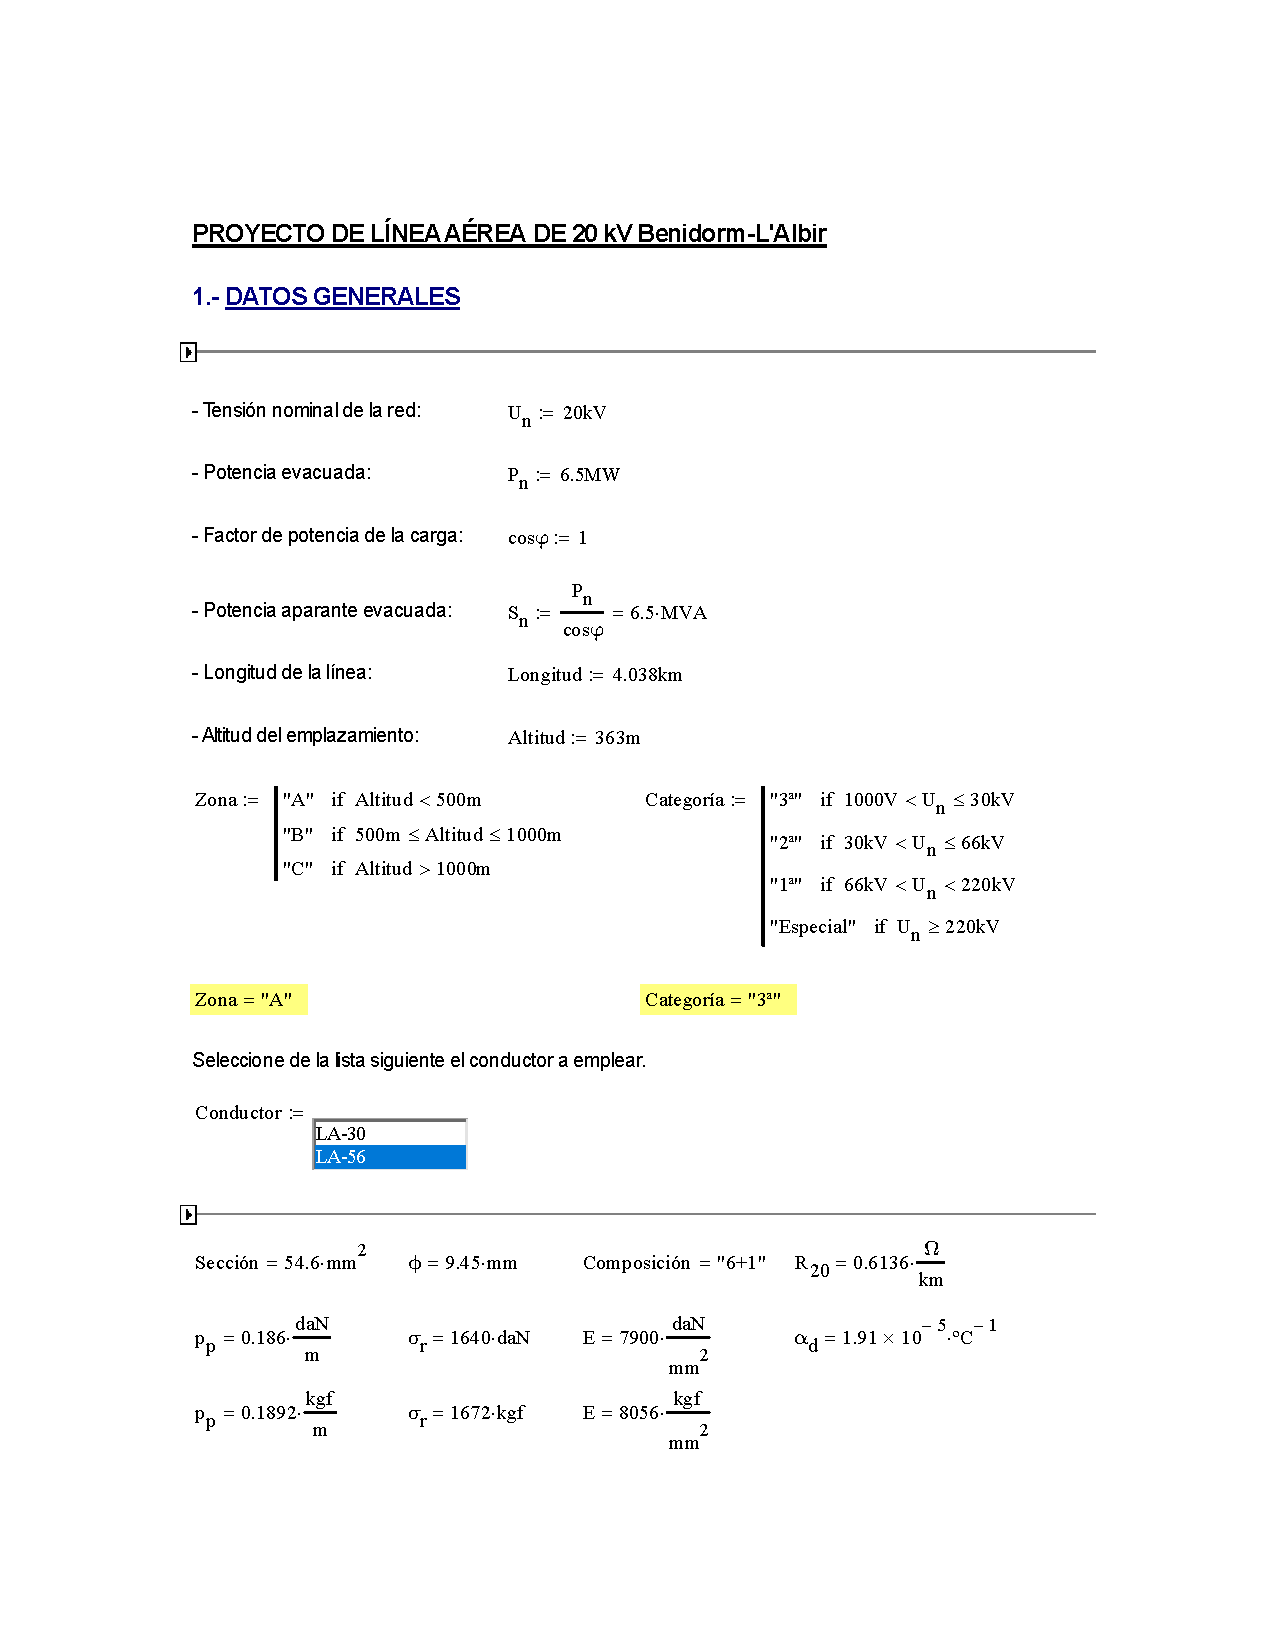
\includepdf[
  pages=1-88,          
  fitpaper=true,    
]{PDFs/mathcad-def.pdf}  

\clearpage
\chapter*{Anexo B. Cálculos con IMEDEXSA}
\addcontentsline{toc}{chapter}{\textsf{\textbf{Anexo B. Cálculos con IMEDEXSA}}}
\label{anexo:imedexsa}
% Anexos/imedexsa.tex

% Ejemplo: incluir un PDF entero (todas las páginas)
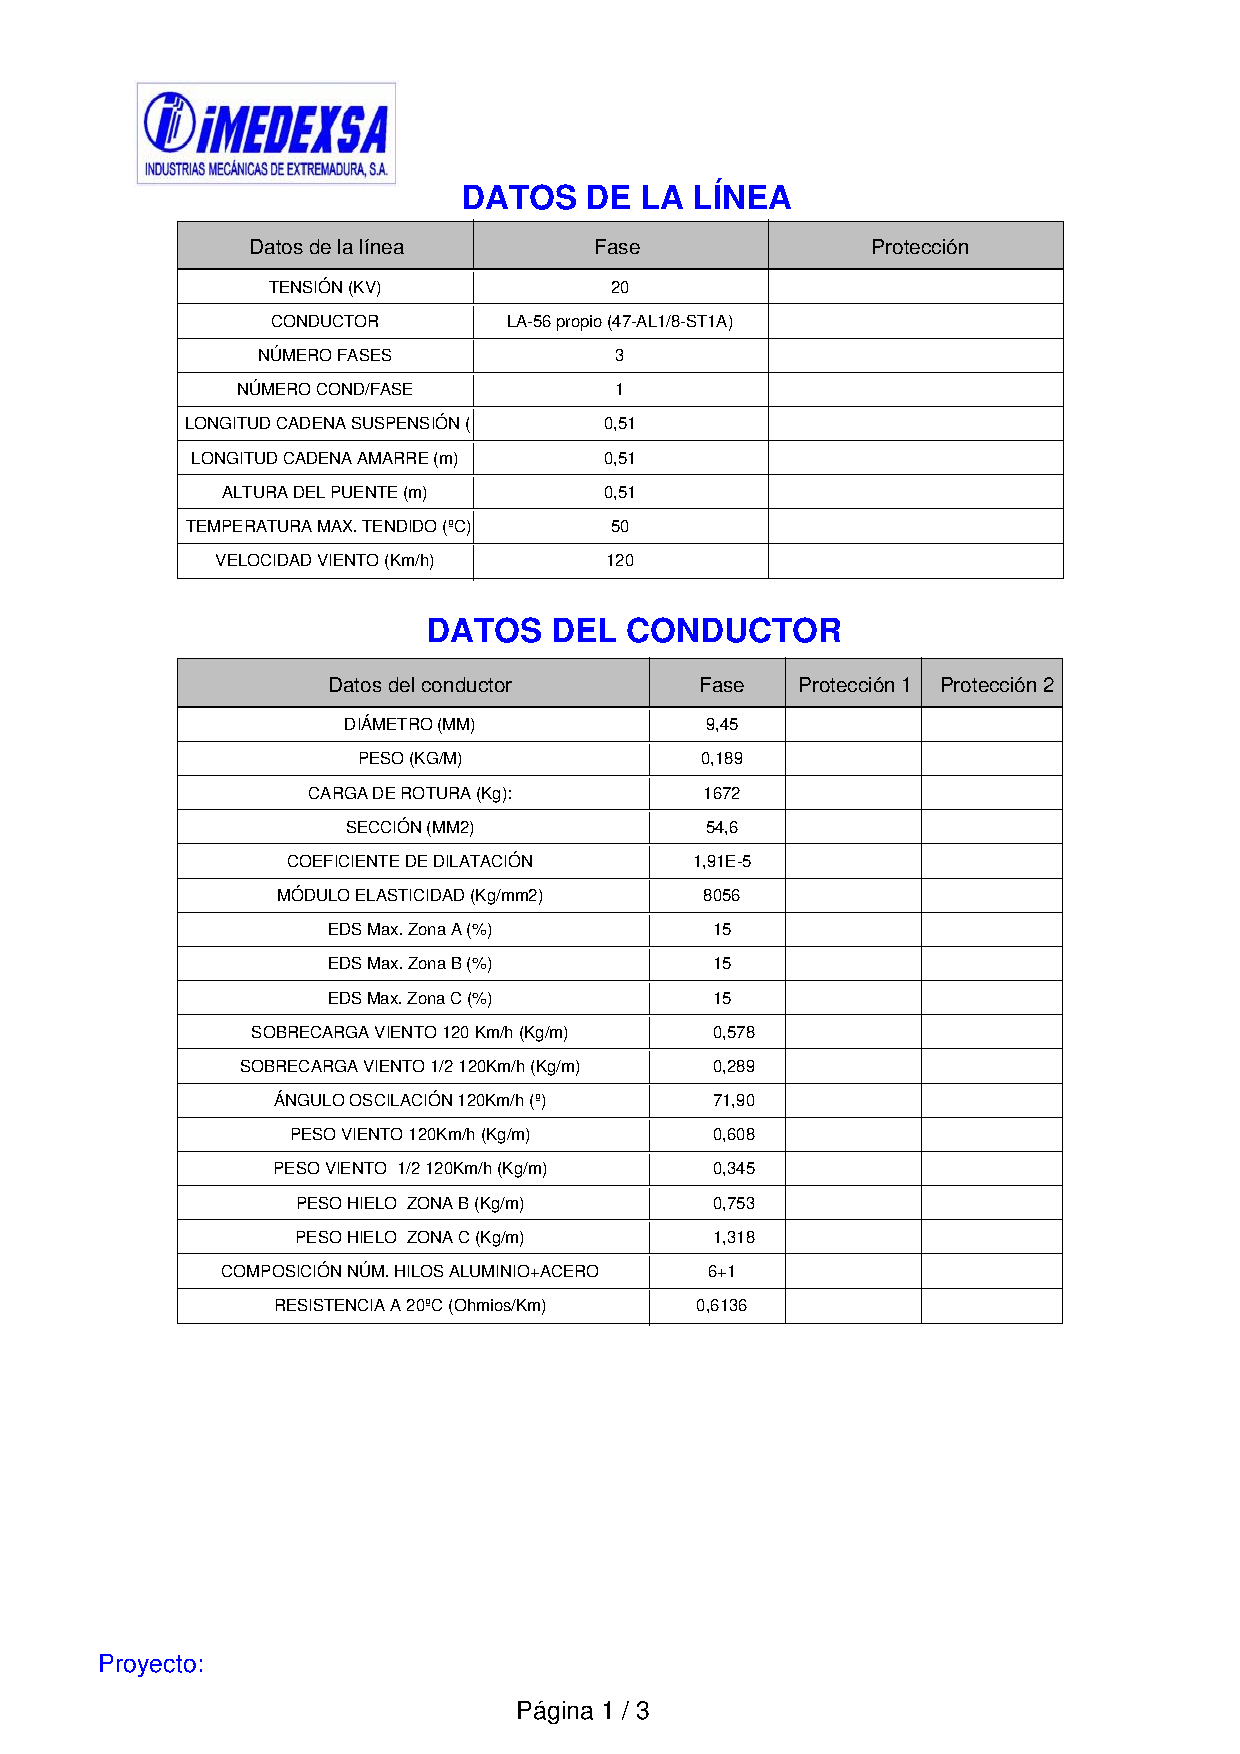
\includepdf[
  pages=-,          % todas las páginas
  fitpaper=true,    % ajusta al tamaño del papel del documento
]{PDFs/ANEXO 1 Datos Generales.pdf}

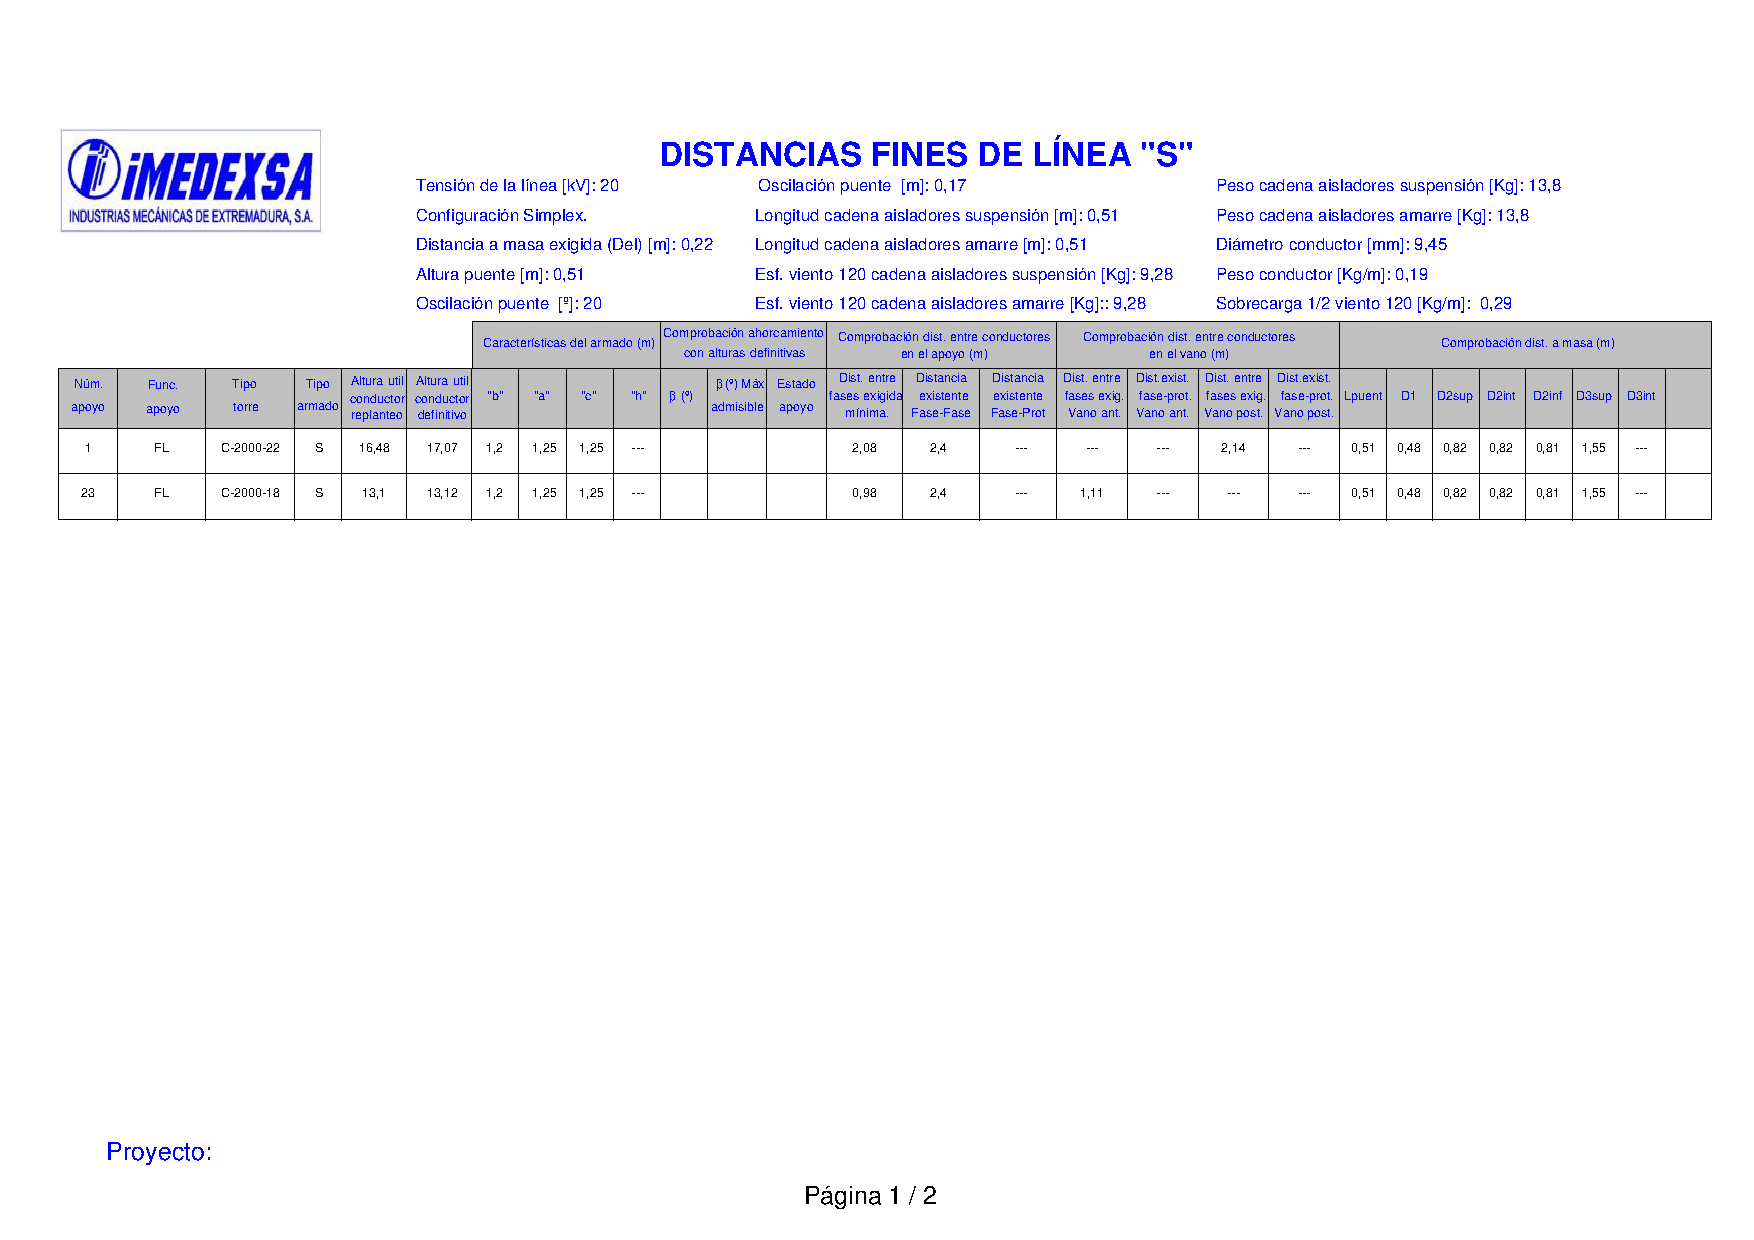
\includepdf[
  pages=-,          
  fitpaper=true,    
]{PDFs/ANEXO 2.1 Distancias FINES DE LÍNEA S.pdf}

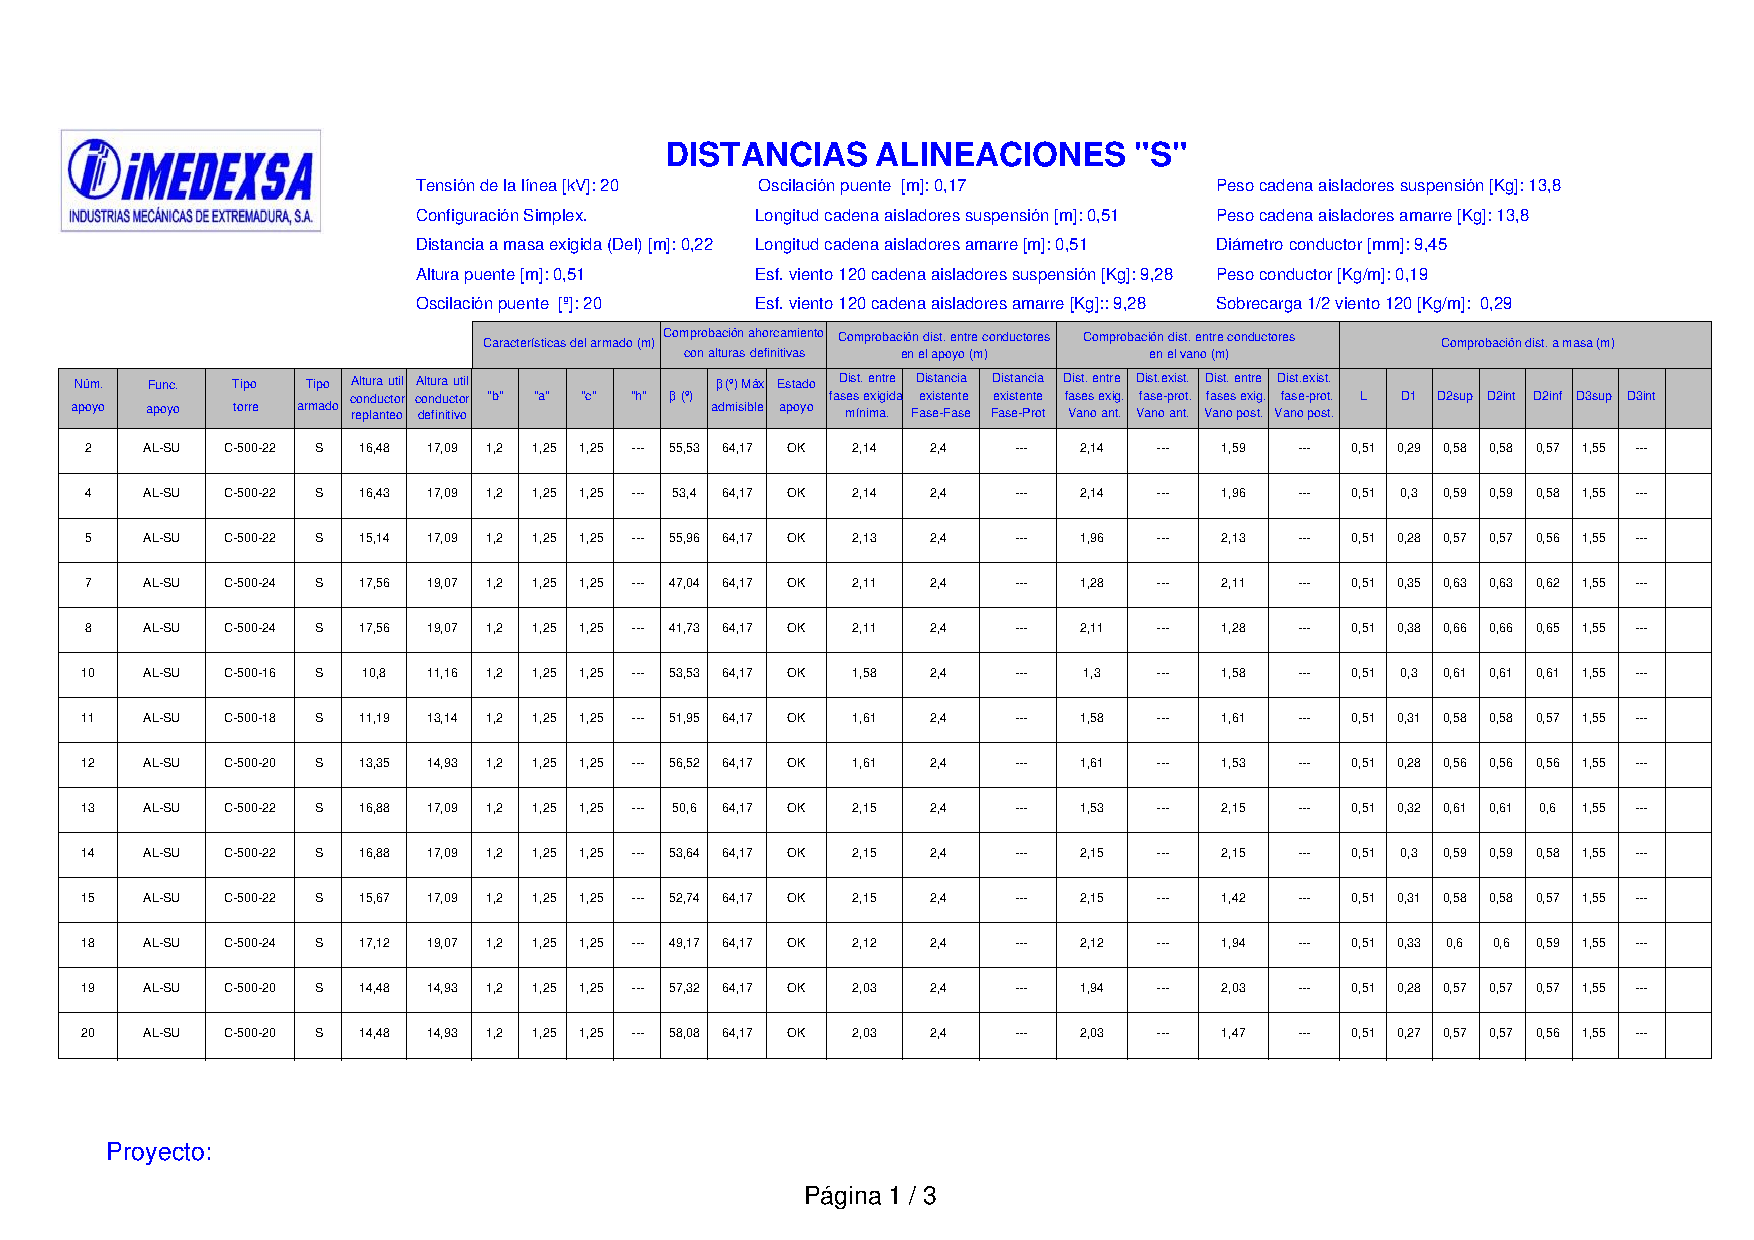
\includepdf[
  pages=-,          
  fitpaper=true,      
]{PDFs/ANEXO 2.2 Distancias ALINEACIONES S.pdf}

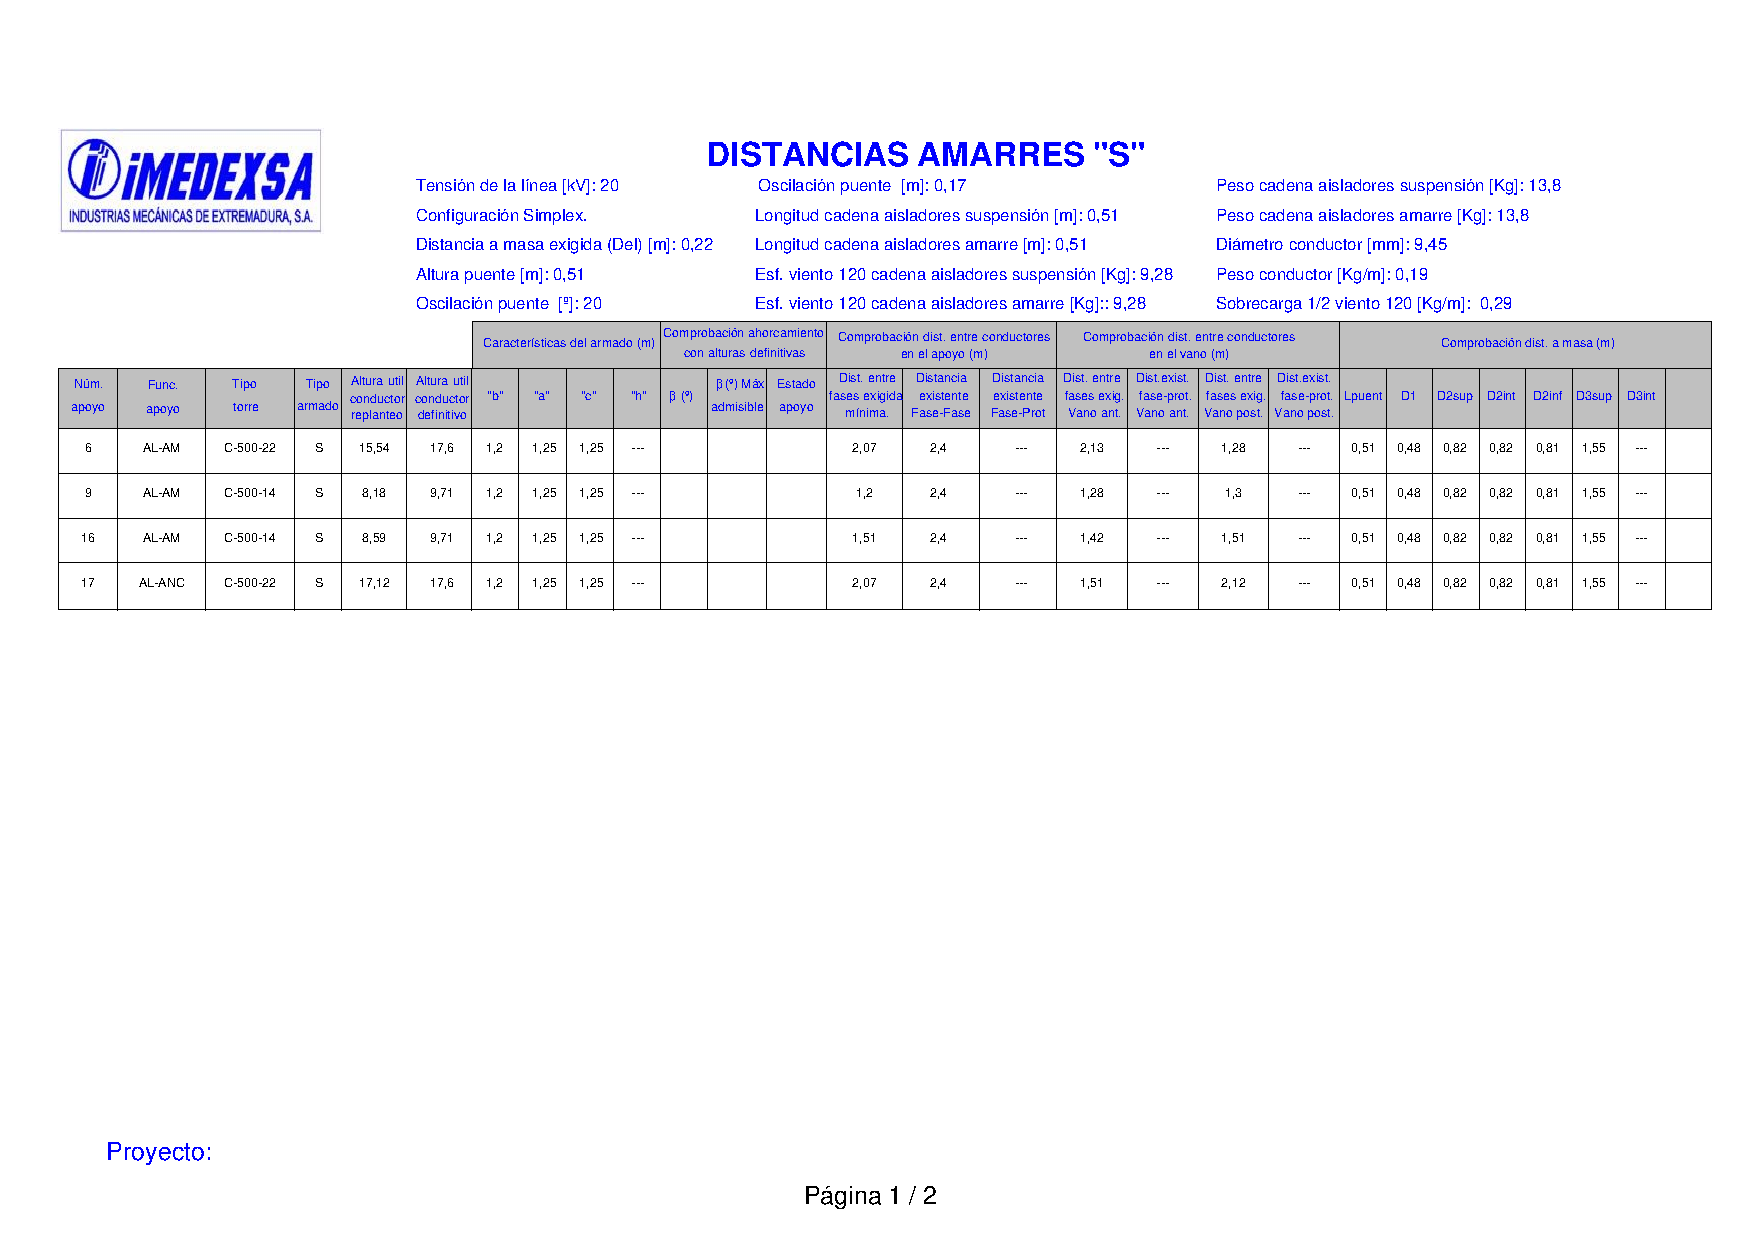
\includepdf[
  pages=-,          
  fitpaper=true,      
]{PDFs/ANEXO 2.3 Distancias AMARRES S.pdf}

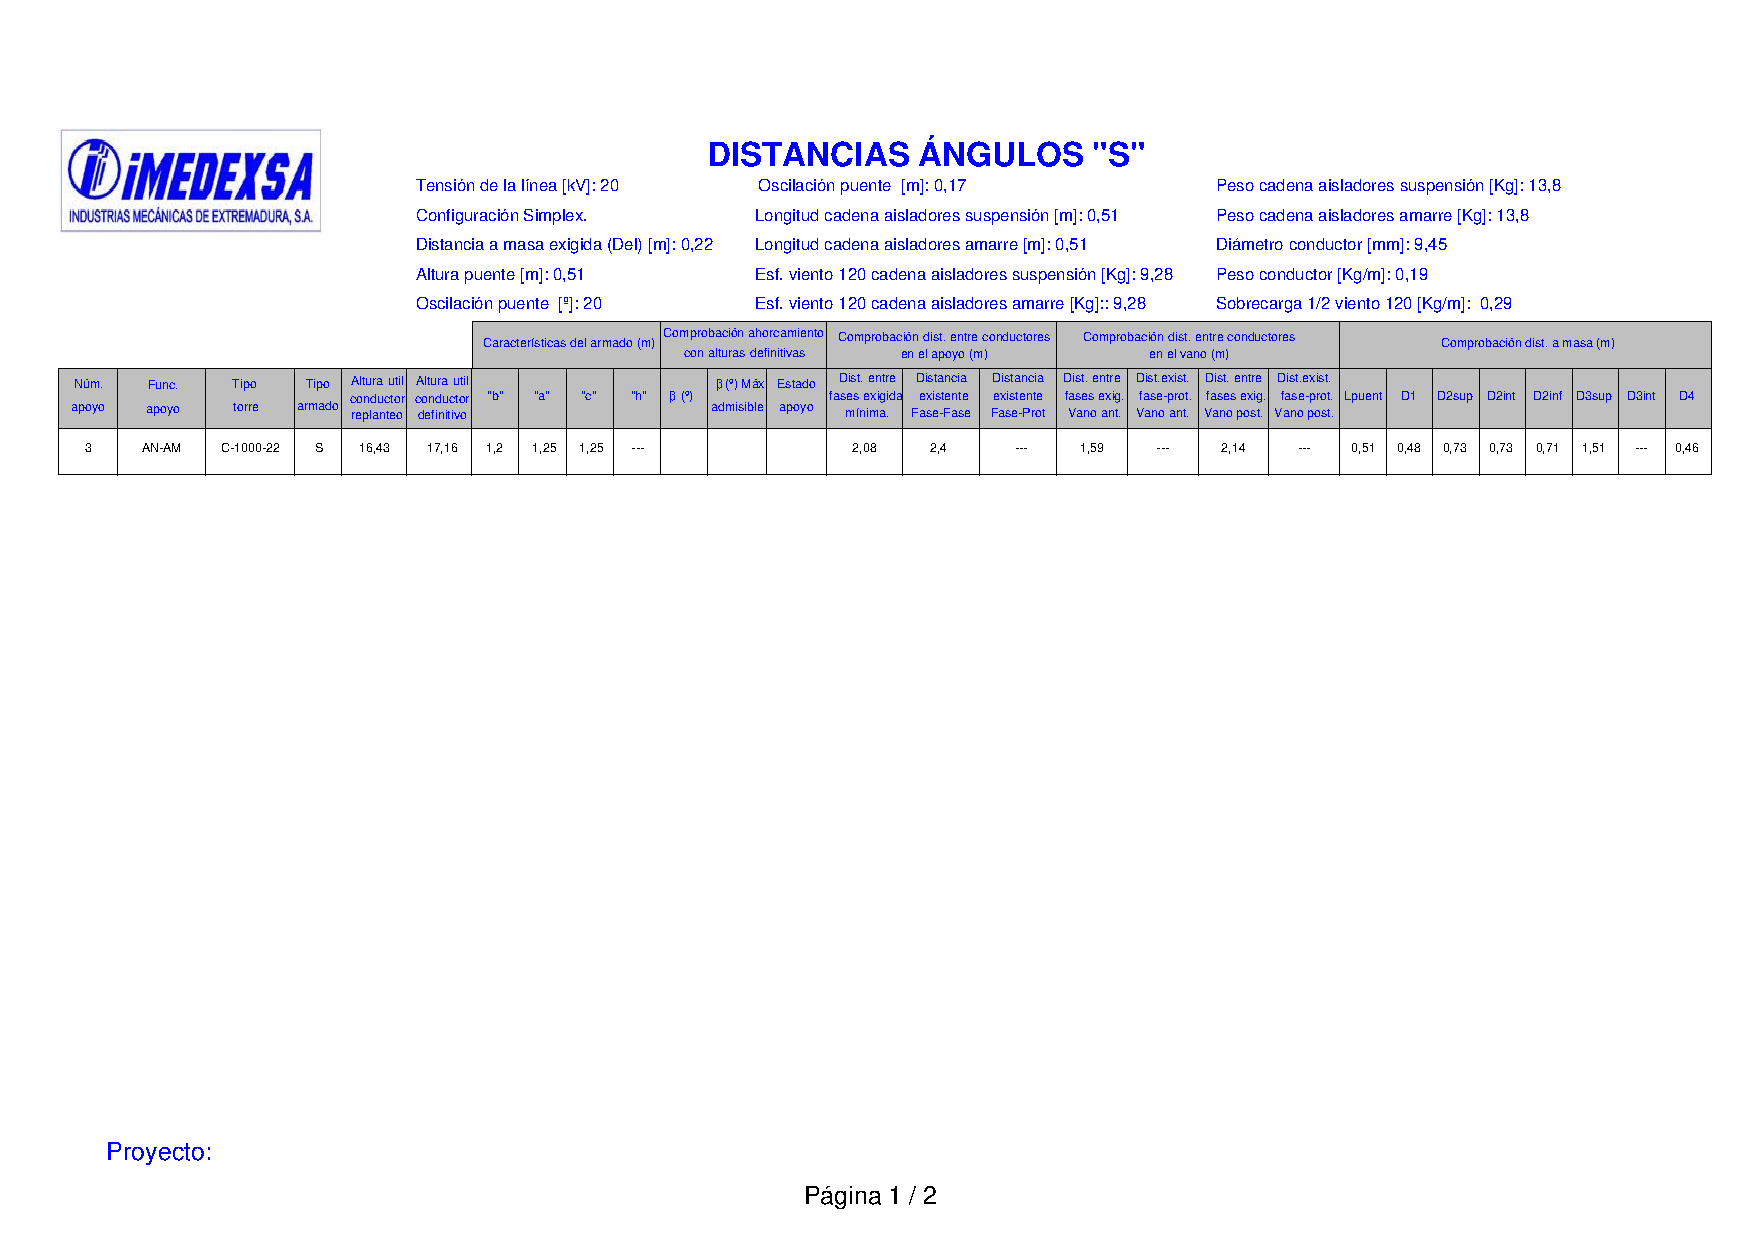
\includepdf[
  pages=-,          
  fitpaper=true,     
]{PDFs/ANEXO 2.4 Distancias ÁNGULOS S.pdf}

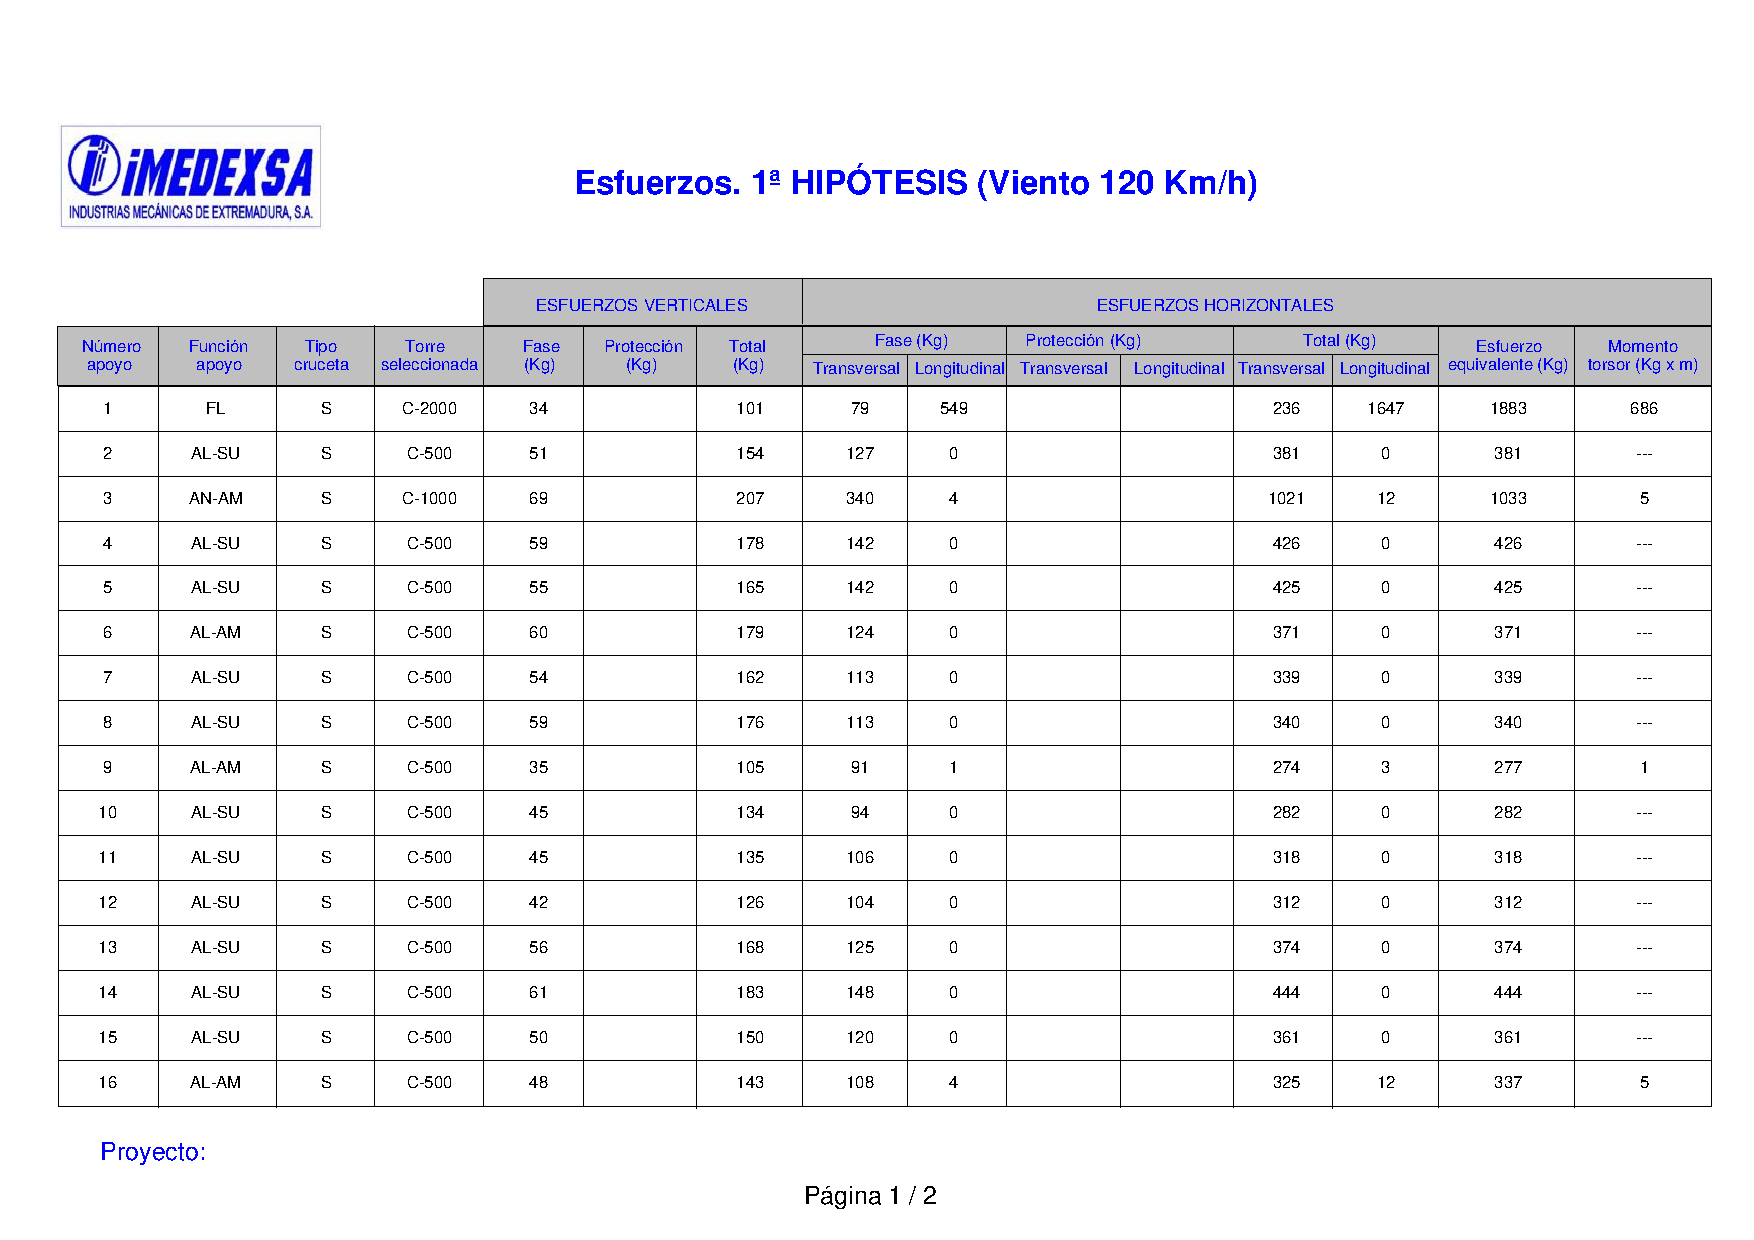
\includepdf[
  pages=-,          
  fitpaper=true,      
]{PDFs/ANEXO 3.1 Esfuerzos PRIMERA.pdf}

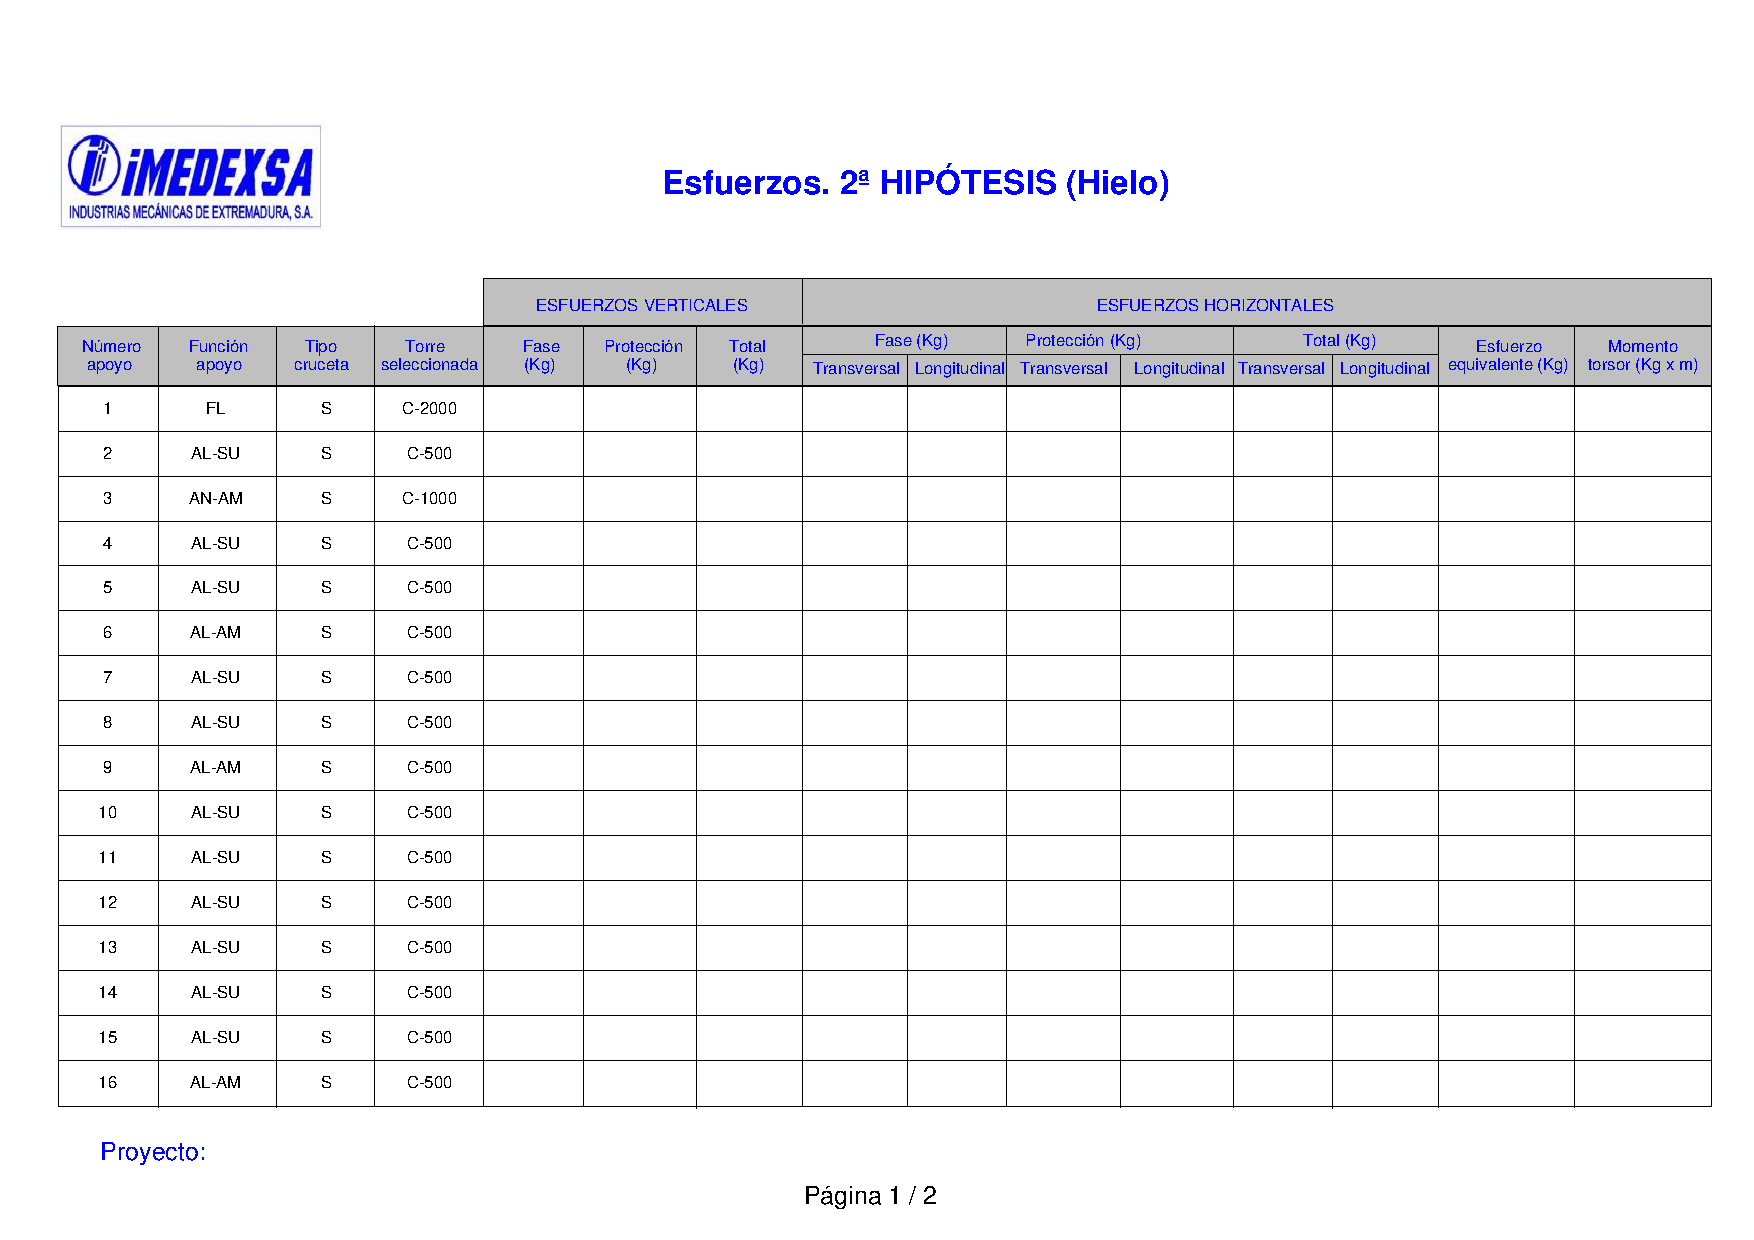
\includepdf[
  pages=-,          
  fitpaper=true,      
]{PDFs/ANEXO 3.2 Esfuerzos SEGUNDA.pdf}

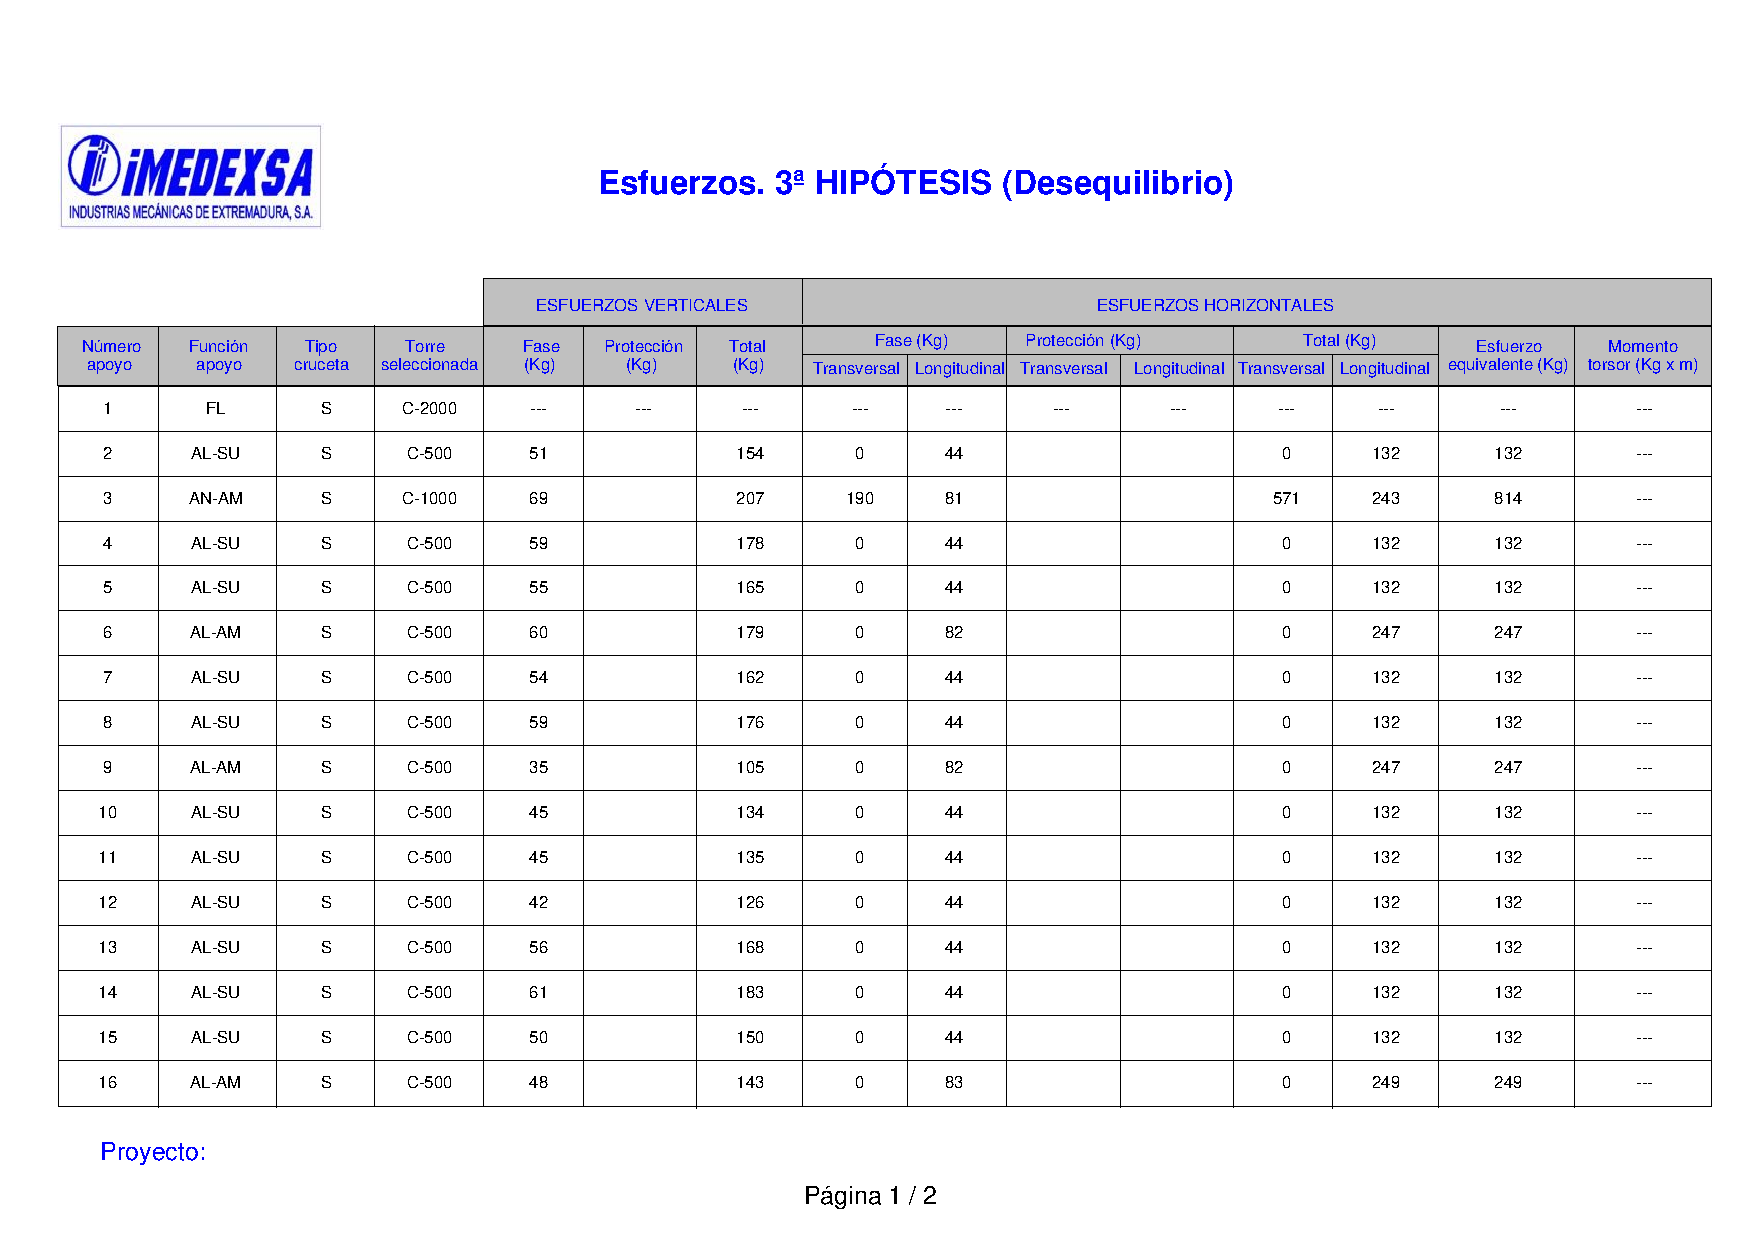
\includepdf[
  pages=-,          
  fitpaper=true,      
]{PDFs/ANEXO 3.3 Esfuerzos TERCERA.pdf}

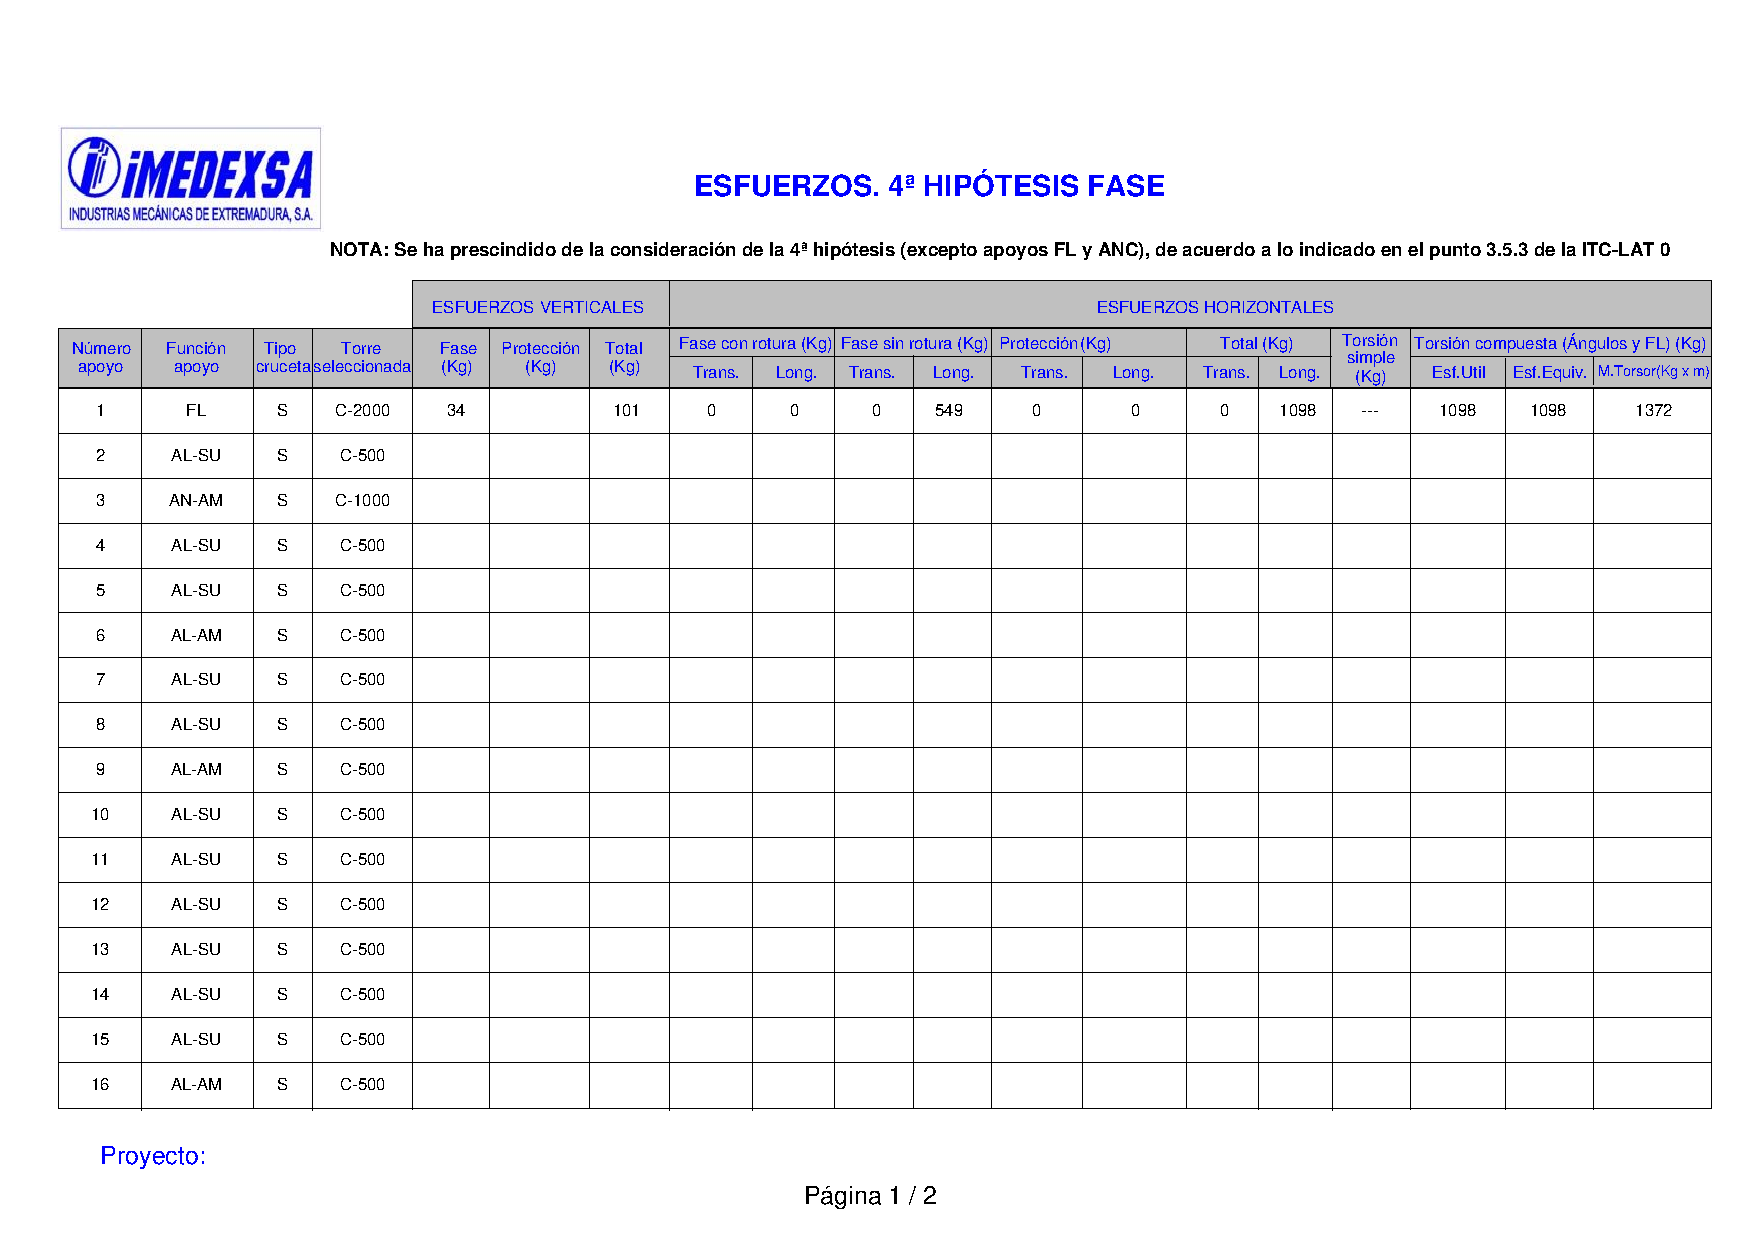
\includepdf[
  pages=-,          
  fitpaper=true,      
]{PDFs/ANEXO 3.4 Esfuerzos CUARTA FASE.pdf}

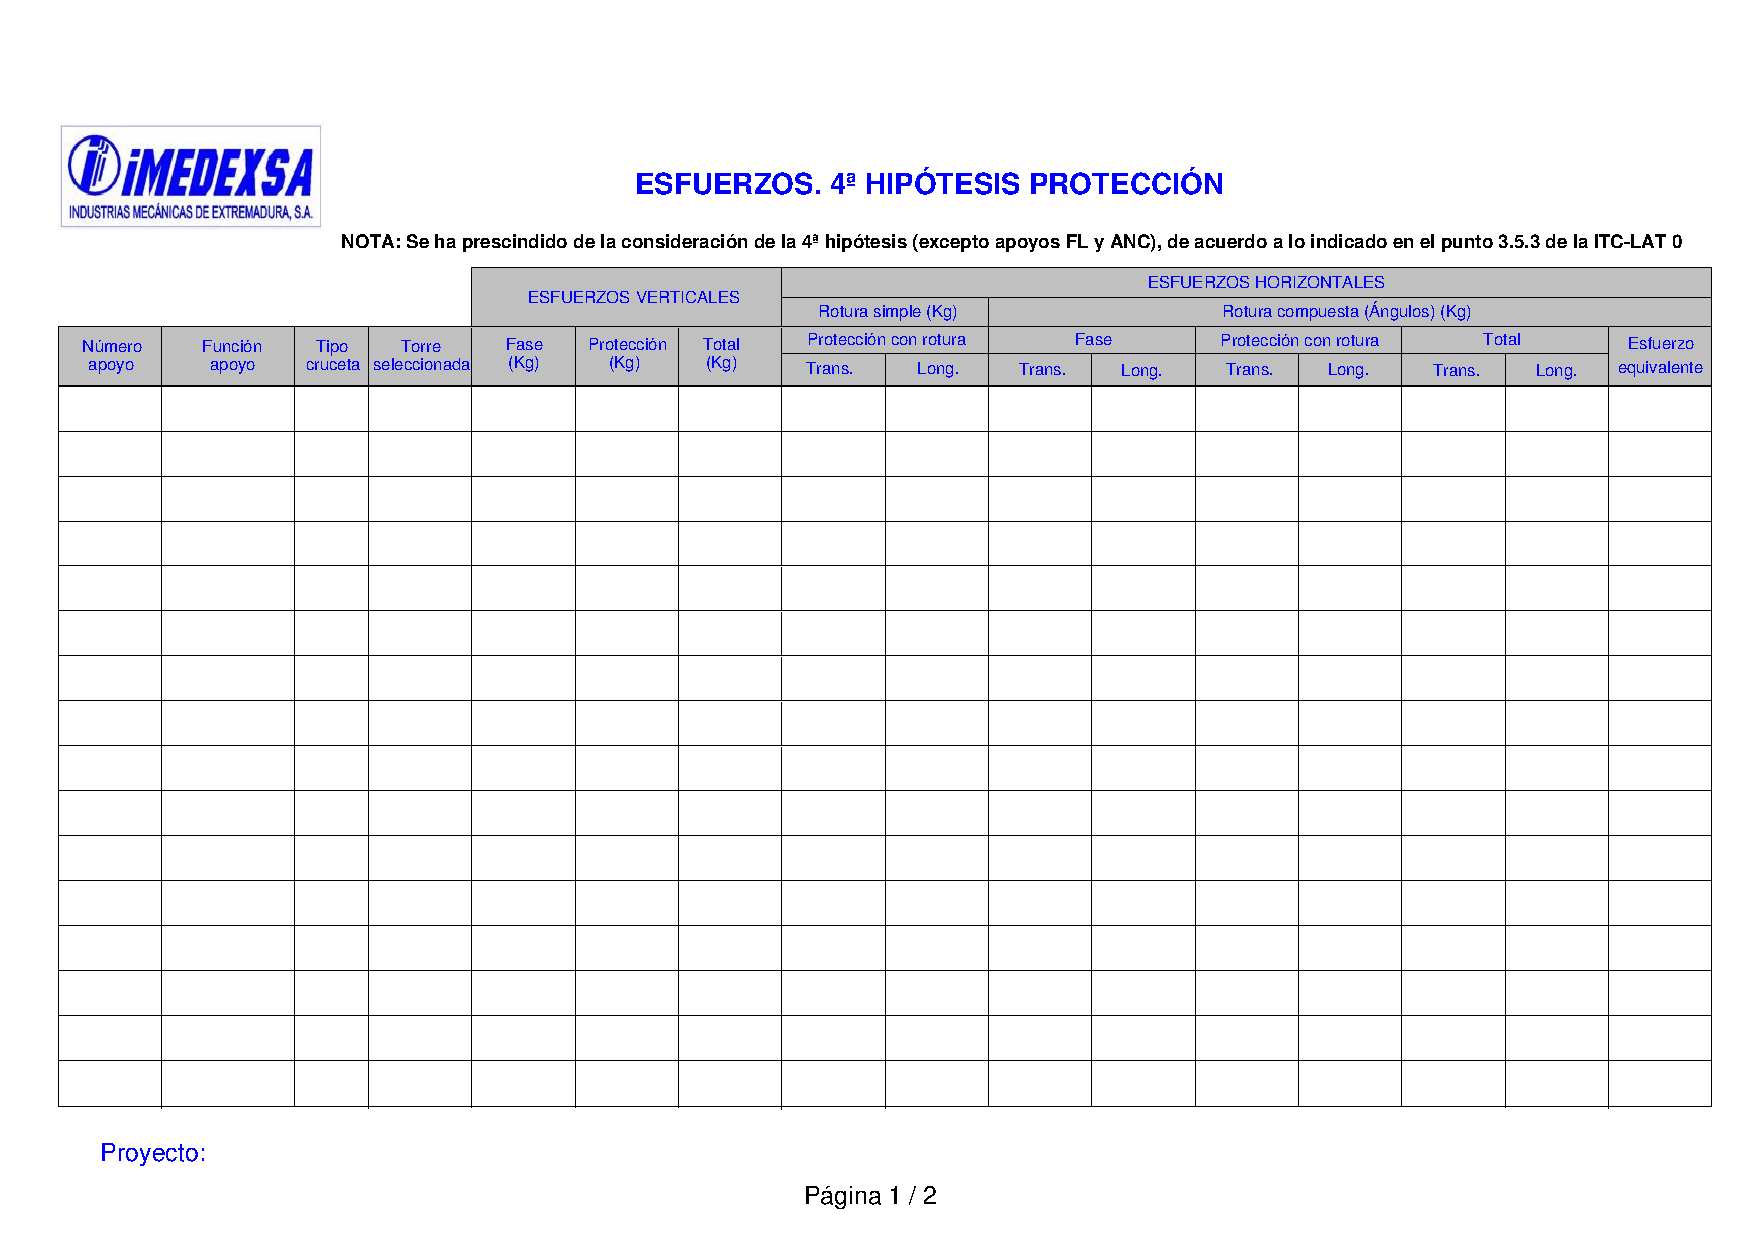
\includepdf[
  pages=-,          
  fitpaper=true,     
]{PDFs/ANEXO 3.5 Esfuerzos CUARTA PROTECCIÓN.pdf}

\includepdf[
  pages=1-2,          
  fitpaper=true,    
]{PDFs/ANEXO 4 Detalles de apoyos.pdf}

\includepdf[
  pages=3-25,          
  fitpaper=true,      
]{PDFs/ANEXO 4 Detalles de apoyos.pdf}

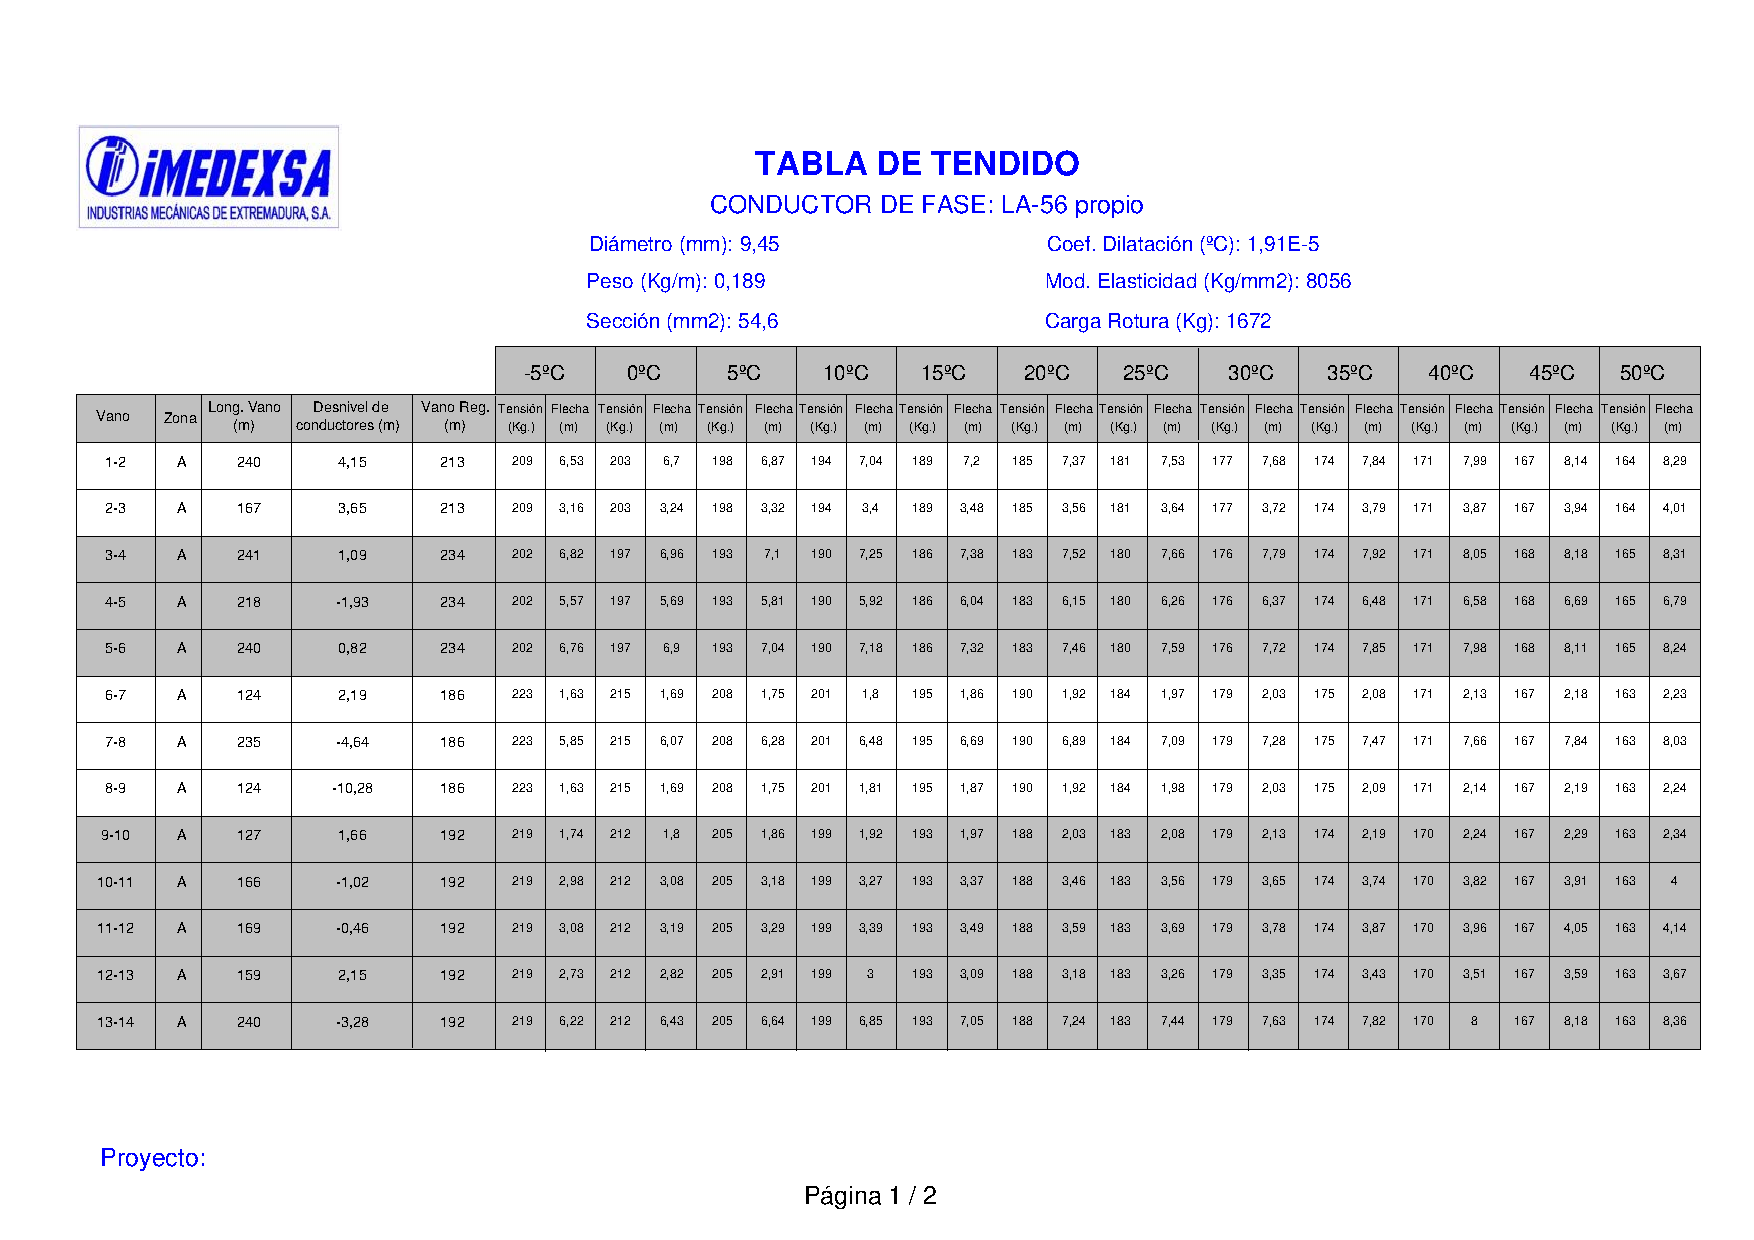
\includepdf[
  pages=-,          
  fitpaper=true,      
]{PDFs/ANEXO 5 TABLA TENDIDO FASE.pdf}

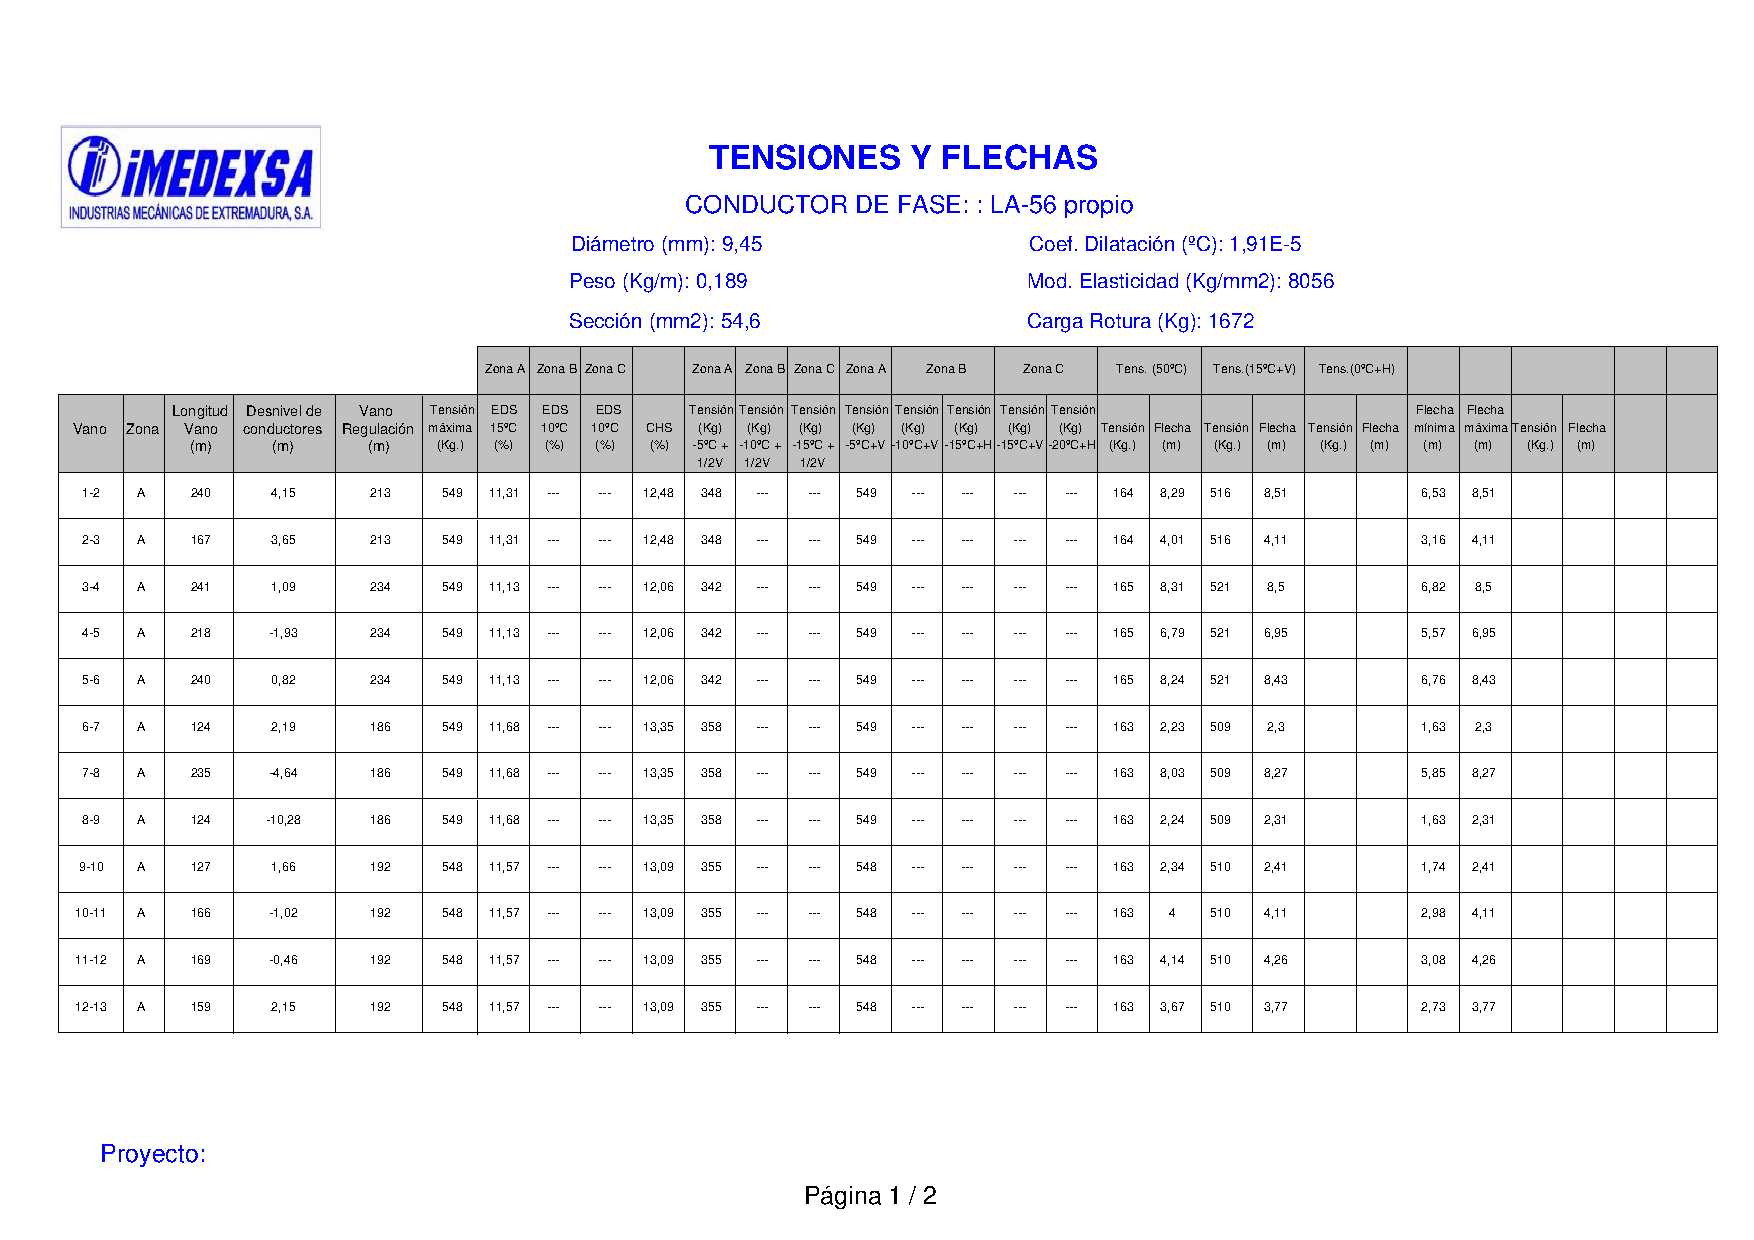
\includepdf[
  pages=-,          
  fitpaper=true,      
]{PDFs/ANEXO 6 TENSIONES Y FLECHAS FASE.pdf}

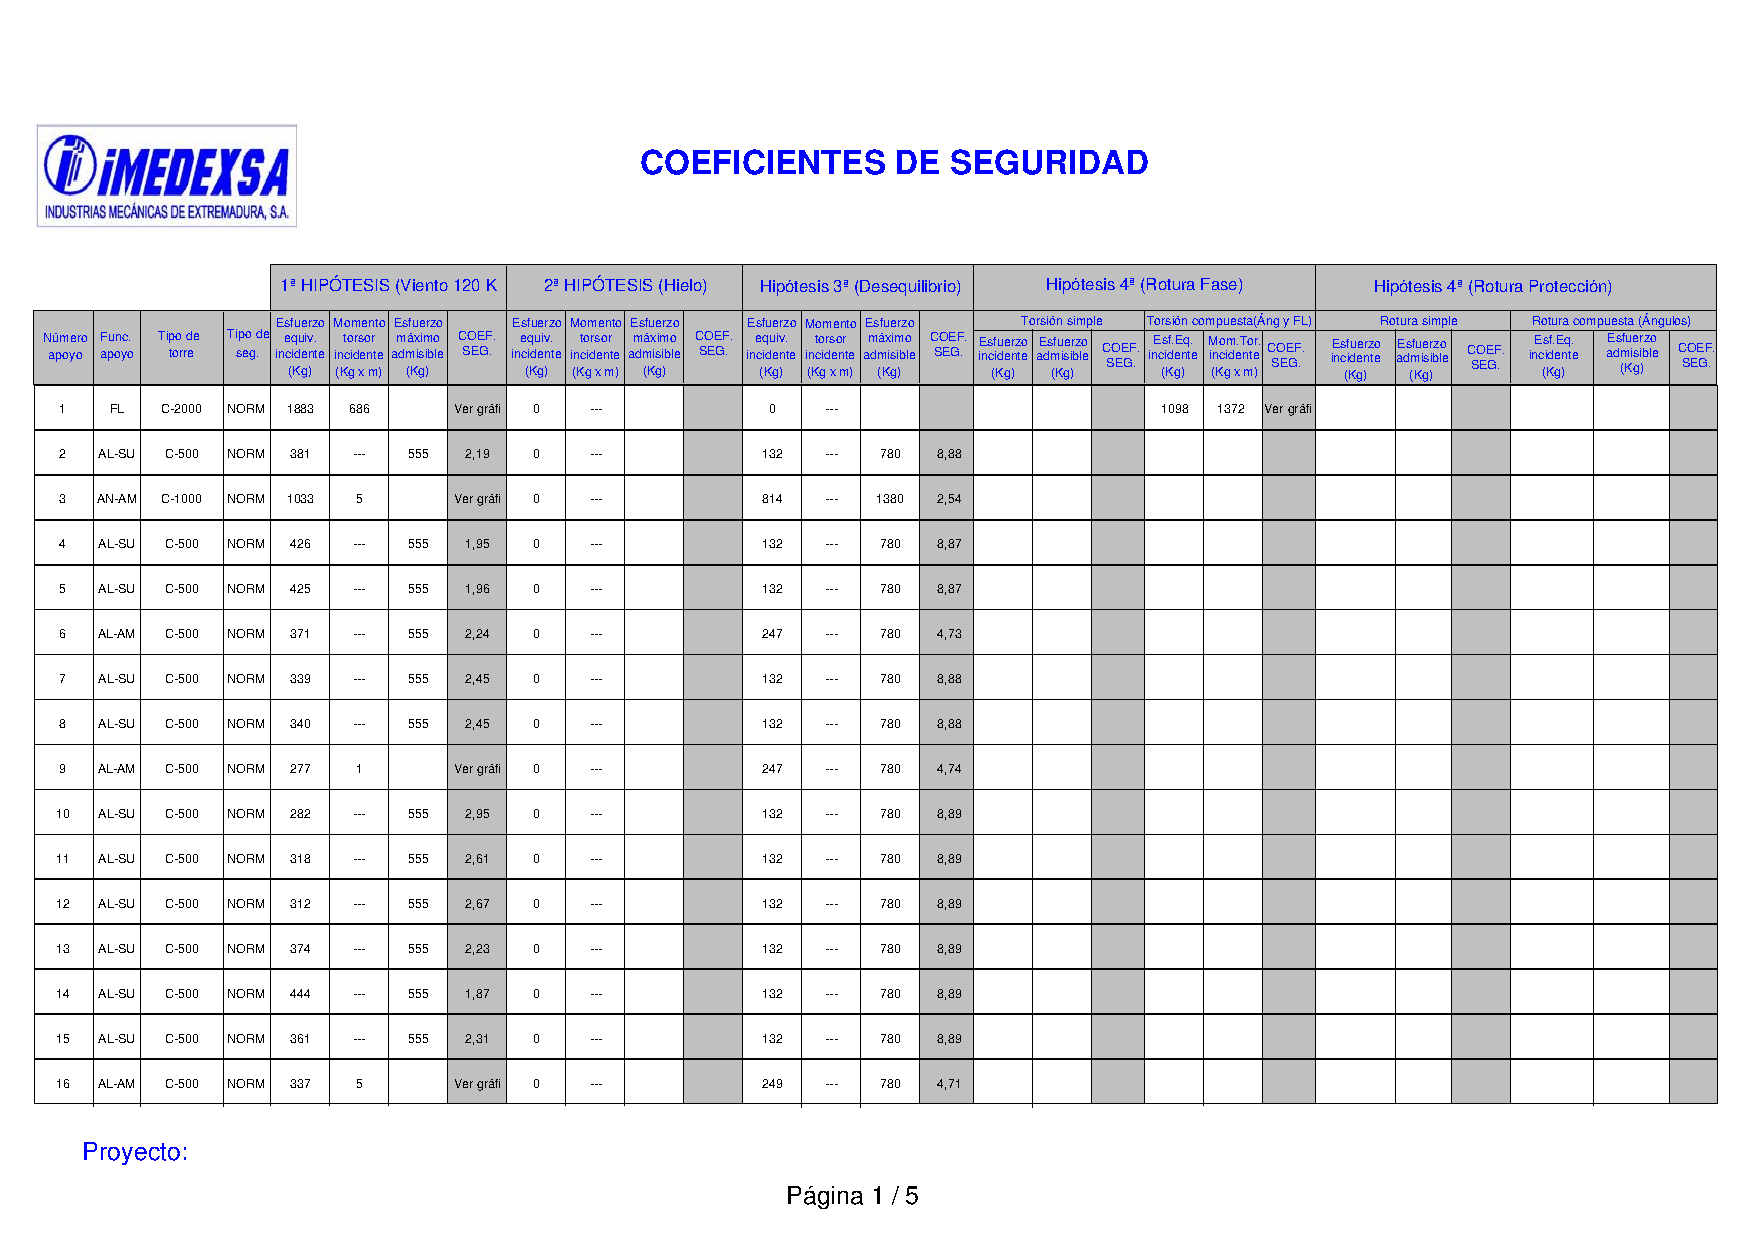
\includepdf[
  pages=1-2,          
  fitpaper=true,
]{PDFs/ANEXO 7 Coeficientes de seguridad.pdf}

\includepdf[
  pages=3-5,          
  fitpaper=true,
]{PDFs/ANEXO 7 Coeficientes de seguridad.pdf}

\includepdf[
  pages=1-3,          
  fitpaper=true,       
]{PDFs/ANEXO 8 CIMENTACIONES.pdf}

\includepdf[
  pages=4-26,          
  fitpaper=true,      
]{PDFs/ANEXO 8 CIMENTACIONES.pdf}

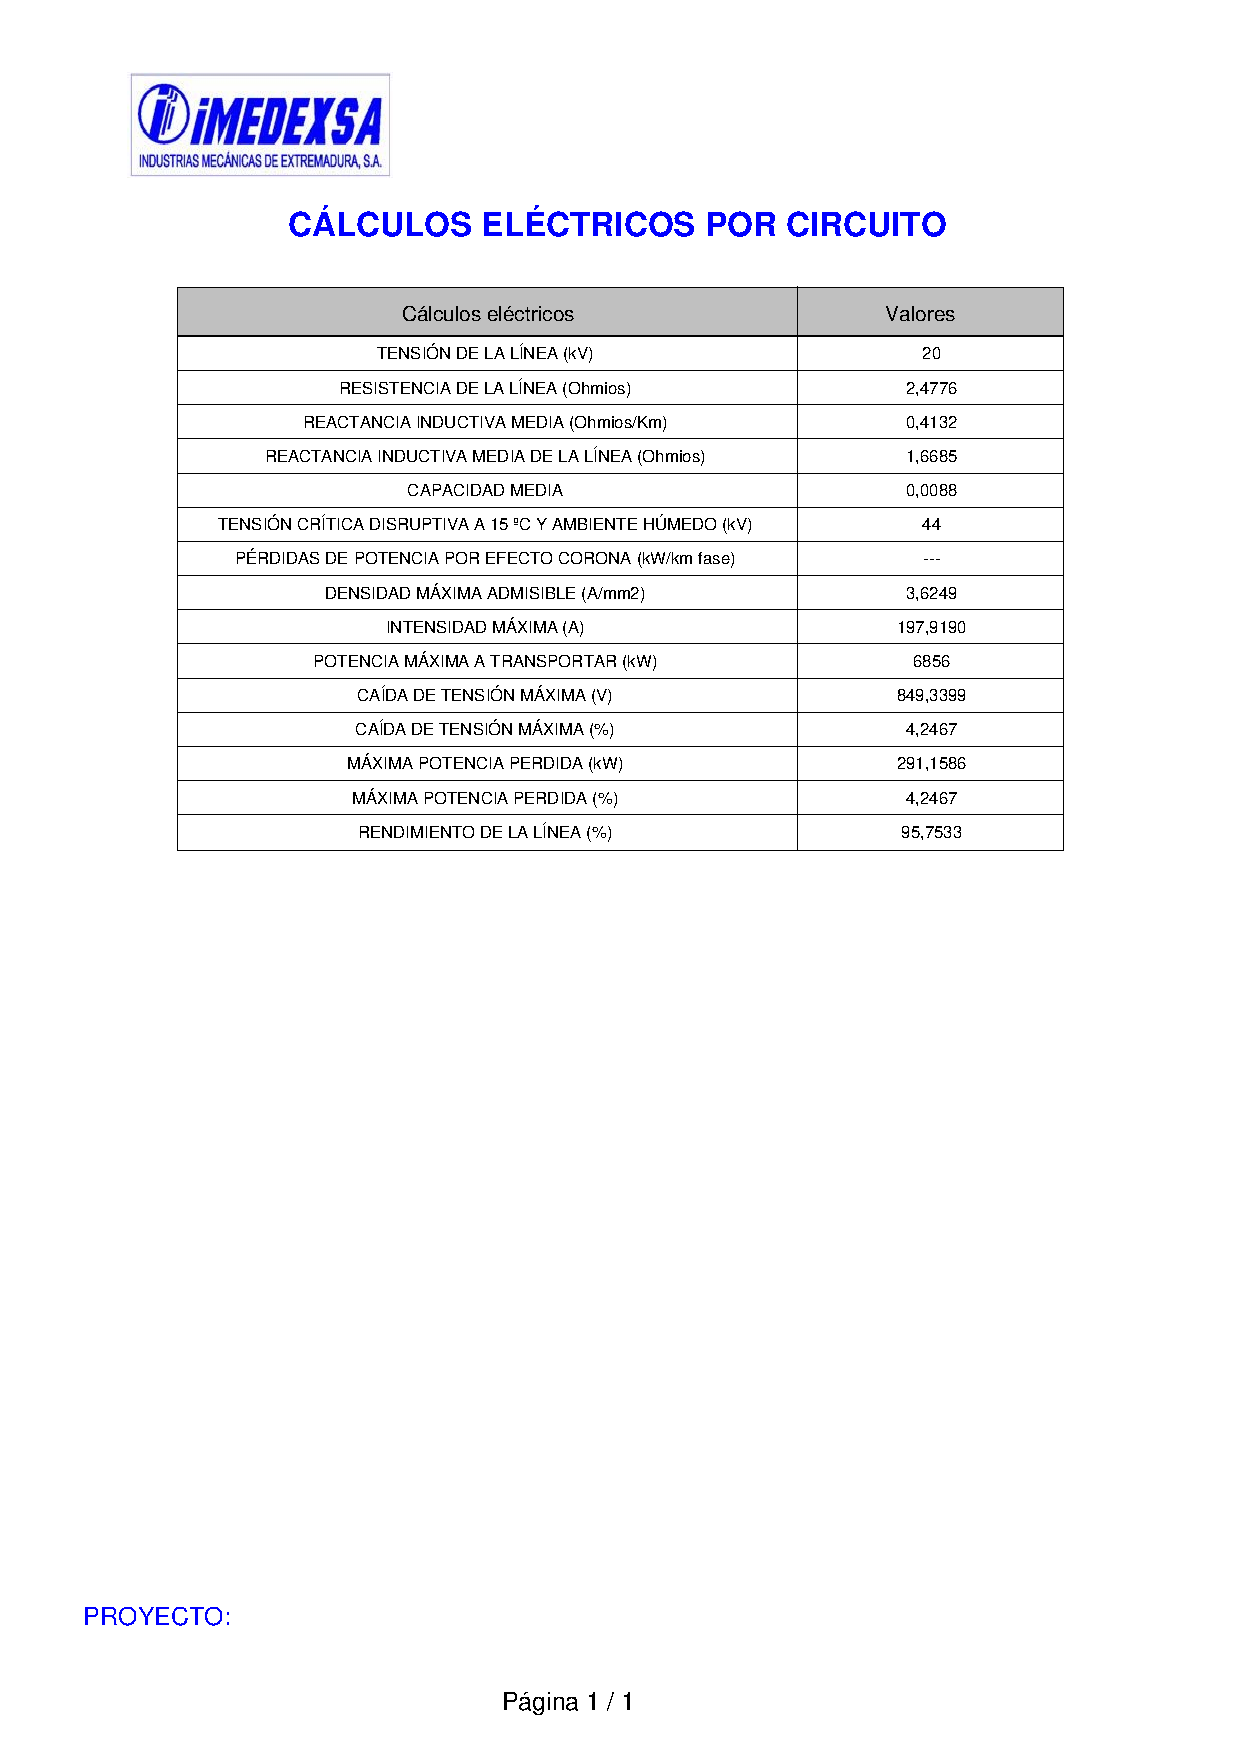
\includepdf[
  pages=-,          
  fitpaper=true,     
]{PDFs/ANEXO 9 CÁLCULOS ELÉCTRICOS.pdf}

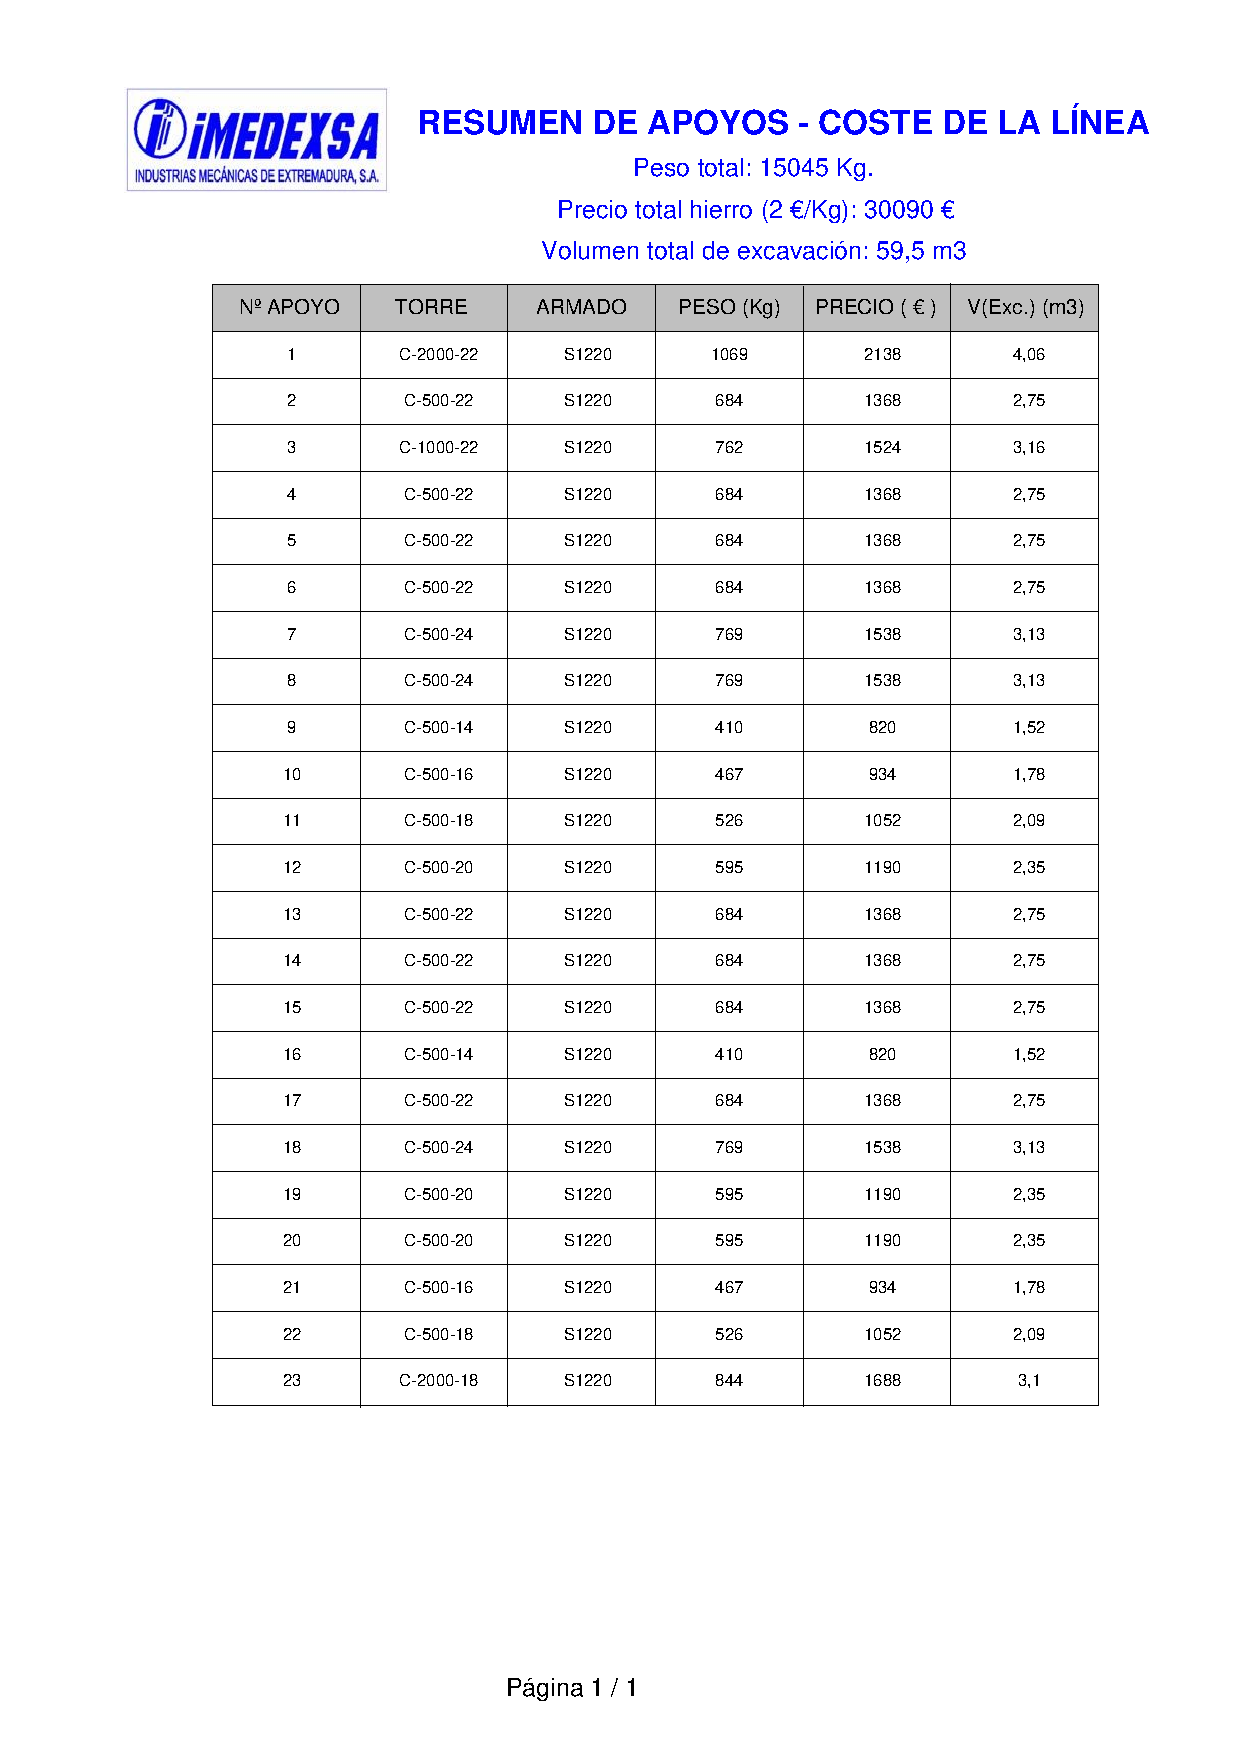
\includepdf[
  pages=-,          
  fitpaper=true,     
]{PDFs/ANEXO 10 Resumen de costes.pdf}

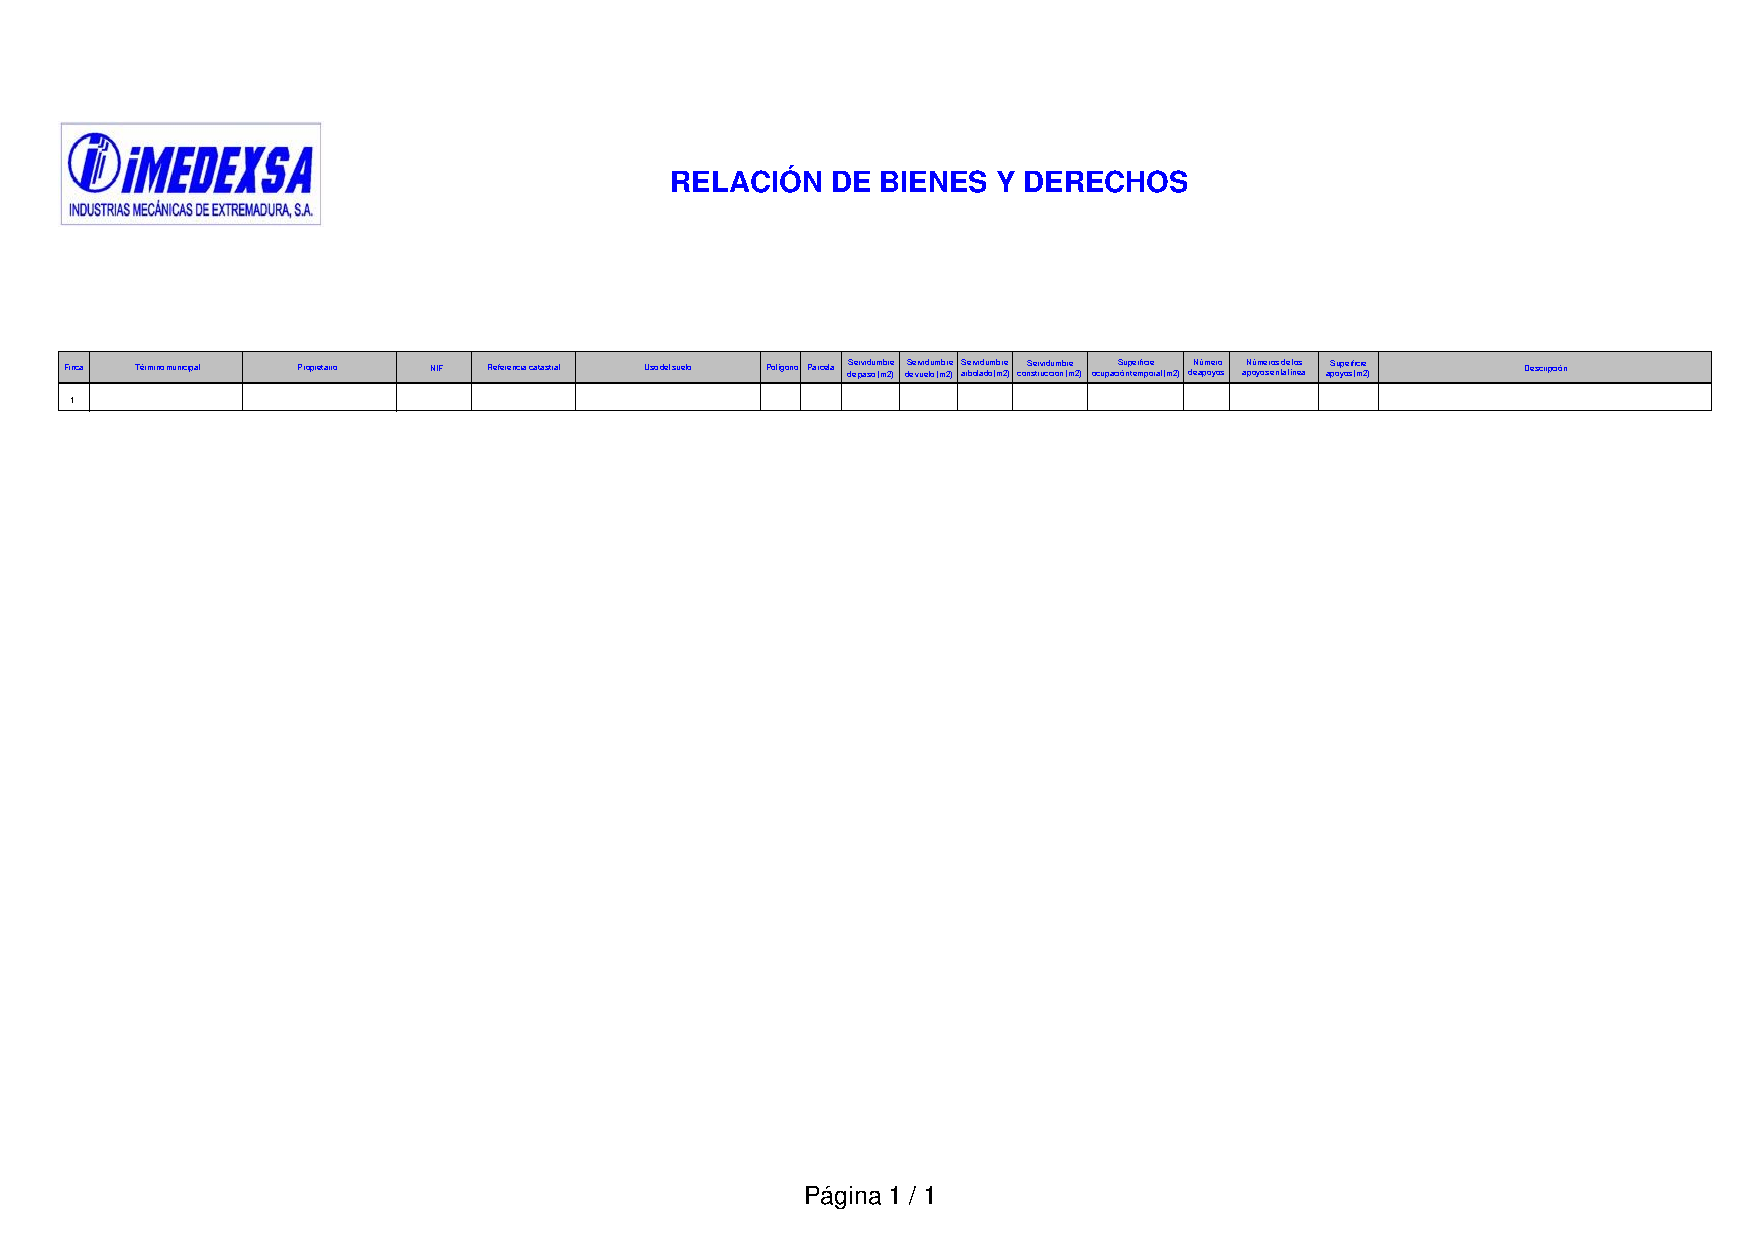
\includepdf[
  pages=-,          
  fitpaper=true,       
]{PDFs/ANEXO 11 Parcelas.pdf}

% Ejemplo: incluir solo páginas concretas
%\includepdf[
%  pages={1,3-5},
%  fitpaper=true,
%  pagecommand={}
%]{PDFs/imedexsa_calculos.pdf}
 


\end{document}